%   D O C U M E N T   P R E A M B L E
% Specify the document class, default style attributes, and page dimensions, etc.
% For hyperlinked PDF, suitable for viewing on a computer, use this:
\documentclass[letterpaper,12pt,titlepage,oneside,final,usenames,dvipsnames]{book}

% \usepackage{XCharter}
% \renewcommand{\rmdefault}{XCharter}
% \usepackage{textcomp} % Add the textcomp package

 
% For PDF, suitable for double-sided printing, change the PrintVersion variable below to "true" and use this \documentclass line instead of the one above:
%\documentclass[letterpaper,12pt,titlepage,openright,twoside,final]{book}

% Some LaTeX commands I define for the document nomenclature.
\newcommand{\die}[2]{\frac{\partial #1}{\partial #2}}
\newcommand{\package}[1]{\textbf{#1}} % package names in bold text
\newcommand{\cmmd}[1]{\textbackslash\texttt{#1}} % command name in tt font 
\newcommand{\href}[1]{#1} % does nothing, but defines the command so the print-optimized version will ignore \href tags (redefined by hyperref pkg).
%\newcommand{\texorpdfstring}[2]{#1} % does nothing, but defines the command
% Anything defined here may be redefined by packages added below...
% This package allows if-then-else control structures.
\usepackage{ifthen}
\newboolean{PrintVersion}
\setboolean{PrintVersion}{false}
% CHANGE THIS VALUE TO "true" as necessary, to improve printed results for hard copies by overriding some options of the hyperref package, called below.

%\usepackage{nomencl} % For a nomenclature (optional; available from ctan.org)
\usepackage{amsmath,amssymb,amstext} % Lots of math symbols and environments
\usepackage[pdftex]{graphicx} % For including graphics N.B. pdftex graphics driver 

%----------------------------------------------------------------------
%   A D D  H E R E
% Packages added for Kirsten's dissertation
% \usepackage{geometry}
\usepackage{changepage}
\usepackage{epigraph}
\setlength\epigraphwidth{.8\textwidth}
\usepackage[absolute]{textpos}
\usepackage{lmodern}% DRR adde d for sizin text in tikz
% \usepackage{setspace}
% \usepackage{xcolor, tikz}
% \usetikzlibrary{chains,fit}
% \usepackage{tikz}
% \usetikzlibrary{shadings, shadows, shapes, arrows, calc, positioning, shapes.geometric, arrows.meta, patterns, patterns.meta}
\usepackage{xcolor, tikz}
\usetikzlibrary{chains,fit, shadings, shadows, shapes, shapes.geometric, arrows, calc, positioning, shapes.geometric, arrows.meta, patterns, patterns.meta}

\tikzstyle{startstop} = [rectangle, rounded corners, minimum width=3cm, minimum height=1cm,text centered, draw=black, fill=red!30]
\tikzstyle{process} = [rectangle, minimum width=3cm, minimum height=1cm, text centered, draw=black, fill=orange!30]
\tikzstyle{decision} = [rectangle, minimum width=3cm, minimum height=1cm, text centered, draw=black, fill=green!30]
\tikzstyle{arrow} = [thick,->,>=stealth]

\usepackage{listings}

\definecolor{codegreen}{rgb}{0,0.6,0}
\definecolor{codegray}{rgb}{0.5,0.5,0.5}
\definecolor{codepurple}{rgb}{0.58,0,0.82}
\definecolor{backcolour}{rgb}{0.95,0.95,0.92}

% Code style examples 
% https://github.com/srinadhu/RL_Pacman/blob/master/report.pdf
% https://www.overleaf.com/learn/latex/Code_listing

\lstdefinestyle{mystyle}{
    language=Python,
    backgroundcolor=\color{backcolour},   
    commentstyle=\color{codegreen},
    keywordstyle=\color{magenta},
    numberstyle=\tiny\color{codegray},
    stringstyle=\color{codepurple},
    basicstyle=\ttfamily\footnotesize,
    breakatwhitespace=false,         
    breaklines=true,                 
    captionpos=b,                    
    keepspaces=true,                 
    numbers=left,                    
    numbersep=5pt,                  
    showspaces=false,                
    showstringspaces=false,
    showtabs=false,                  
    tabsize=2
}

\lstset{style=mystyle}

% \definecolor{dkgreen}{rgb}{0,0.6,0}
% \definecolor{gray}{rgb}{0.5,0.5,0.5}
% \definecolor{mauve}{rgb}{0.58,0,0.82}
% \lstset{frame=tb,
%   language=Java,
%   aboveskip=3mm,
%   belowskip=3mm,
%   showstringspaces=false,
%   columns=flexible,
%   basicstyle={\small\ttfamily},
%   numbers=none,
%   numberstyle=\tiny\color{gray},
%   keywordstyle=\color{blue},
%   commentstyle=\color{dkgreen},
%   stringstyle=\color{mauve},
%   breaklines=true,
%   breakatwhitespace=true,
%   tabsize=3
% }

% \newcommand\pythonstyle{\lstset{
% language=Python,
% basicstyle=\ttm,
% morekeywords={self},              % Add keywords here
% keywordstyle=\ttb\color{deepblue},
% emph={MyClass,__init__},          % Custom highlighting
% emphstyle=\ttb\color{deepred},    % Custom highlighting style
% stringstyle=\color{deepgreen},
% frame=tb,                         % Any extra options here
% showstringspaces=false
% }}

% \usepackage{epstopdf}
\usepackage{catchfilebetweentags}
\usepackage{rotating} %DRR Sidewayas
\DeclareGraphicsRule{.tif}{png}{.png}{`convert #1 `dirname #1`/`basename #1 .tif`.png}
\usepackage{pgfplots}
% Add this line to set the compatibility mode
\pgfplotsset{compat=1.17}
%\usepackage[dvipsnames]{xcolor}
%\setpalette("R4")
%----------------------------------------------------------------------

% Hyperlinks make it very easy to navigate an electronic document.
% In addition, this is where you should specify the thesis title and author as they appear in the properties of the PDF document.
% Use the "hyperref" package 
% N.B. HYPERREF MUST BE THE LAST PACKAGE LOADED; ADD ADDITIONAL PKGS ABOVE
\usepackage[pdftex,pagebackref=false]{hyperref} % with basic options
%\usepackage[pdftex,pagebackref=true]{hyperref}
		% N.B. pagebackref=true provides links back from the References to the body text. This can cause trouble for printing.
\hypersetup{
    plainpages=false,       % needed if Roman numbers in frontpages
    unicode=false,          % non-Latin characters in Acrobat’s bookmarks
    pdftoolbar=true,        % show Acrobat’s toolbar?
    pdfmenubar=true,        % show Acrobat’s menu?
    pdffitwindow=false,     % window fit to page when opened
    pdfstartview={FitH},    % fits the width of the page to the window
%    pdftitle={uWaterloo\ LaTeX\ Thesis\ Template},    % title: CHANGE THIS TEXT!
%    pdfauthor={Author},    % author: CHANGE THIS TEXT! and uncomment this line
%    pdfsubject={Subject},  % subject: CHANGE THIS TEXT! and uncomment this line
%    pdfkeywords={keyword1} {key2} {key3}, % list of keywords, and uncomment this line if desired
    pdfnewwindow=true,      % links in new window
    colorlinks=true,        % false: boxed links; true: colored links
    linkcolor=blue,         % color of internal links
    citecolor=green,        % color of links to bibliography
    filecolor=magenta,      % color of file links
    urlcolor=cyan           % color of external links
}
\ifthenelse{\boolean{PrintVersion}}{   % for improved print quality, change some hyperref options
\hypersetup{	% override some previously defined hyperref options
%    colorlinks,%
    citecolor=black,%
    filecolor=black,%
    linkcolor=black,%
    urlcolor=black}
}{} % end of ifthenelse (no else)

\usepackage[automake,toc,abbreviations]{glossaries-extra} % Exception to the rule of hyperref being the last add-on package
% If glossaries-extra is not in your LaTeX distribution, get it from CTAN (http://ctan.org/pkg/glossaries-extra), 
% although it's supposed to be in both the TeX Live and MikTeX distributions. There are also documentation and 
% installation instructions there.

% Setting up the page margins...
% uWaterloo thesis requirements specify a minimum of 1 inch (72pt) margin at the
% top, bottom, and outside page edges and a 1.125 in. (81pt) gutter margin (on binding side). 
% While this is not an issue for electronic viewing, a PDF may be printed, and so we have the same page layout for both printed and electronic versions, we leave the gutter margin in.
% Set margins to minimum permitted by uWaterloo thesis regulations:
\setlength{\marginparwidth}{0pt} % width of margin notes
% N.B. If margin notes are used, you must adjust \textwidth, \marginparwidth
% and \marginparsep so that the space left between the margin notes and page
% edge is less than 15 mm (0.6 in.)
\setlength{\marginparsep}{0pt} % width of space between body text and margin notes
\setlength{\evensidemargin}{0.125in} % Adds 1/8 in. to binding side of all 
% even-numbered pages when the "twoside" printing option is selected
\setlength{\oddsidemargin}{0.125in} % Adds 1/8 in. to the left of all pages when "oneside" printing is selected, and to the left of all odd-numbered pages when "twoside" printing is selected
\setlength{\textwidth}{6.375in} % assuming US letter paper (8.5 in. x 11 in.) and side margins as above
\raggedbottom

% The following statement specifies the amount of space between paragraphs. Other reasonable specifications are \bigskipamount and \smallskipamount.
\setlength{\parskip}{\medskipamount}

% The following statement controls the line spacing.  
% The default spacing corresponds to good typographic conventions and only slight changes (e.g., perhaps "1.2"), if any, should be made.
\renewcommand{\baselinestretch}{1} % this is the default line space setting

% By default, each chapter will start on a recto (right-hand side) page.
% We also force each section of the front pages to start on a recto page by inserting \cleardoublepage commands.
% In many cases, this will require that the verso (left-hand) page be blank, and while it should be counted, a page number should not be printed.
% The following statements ensure a page number is not printed on an otherwise blank verso page.
\let\origdoublepage\cleardoublepage
\newcommand{\clearemptydoublepage}{%
  \clearpage{\pagestyle{empty}\origdoublepage}}
\let\cleardoublepage\clearemptydoublepage

% Define Glossary terms (This is properly done here, in the preamble and could also be \input{} from a separate file...)
% Main glossary entries---definitions of relevant terminology

% \newglossaryentry{}
% {
% name=,
% description={}
% }
% \newglossaryentry{}
% {
% name=,
% description={}
% }
% \newglossaryentry{}
% {
% name=,
% description={}
% }
% \newglossaryentry{}
% {
% name=,
% description={}
% }

\newglossaryentry{margin}
{
name=margin,
description={edge or boundary. In economics the term has an expanded metaphorically supported technical usage. Ricardo referred to the \gls{extensive margin} as the geographical limit of production and emphasised that that limit was the limit of profitable cultivation. It was where a sensible person would stop expanding the area of cultivation for economic reasons. Later economists extended the notion to the stopping point for all kinds of decisions. Using calculus they identified the conditions under which going farther adding more const more than it added.  Margin   appeared as a metaphor in the adjective  \gls{marginal} and in compound terms like \gls{marginal product}, where it refers to the effect of a small change on some variable  such as a small increase in output  from a small increase fertilizer or labour employed. Focus on such quantities is the main feature of the \gls{marginalist} approach. }
}

\newglossaryentry{consumer surplus}
{
name=consumer surplus,
description={}
}

\newglossaryentry{excess profits}
{
name=excess profits,
description={}
}

\newglossaryentry{free entry}
{
name=free entry,
description={}
}

\newglossaryentry{the second circuit of capital}
{
name=the second circuit of capital,
description={}
}

\newglossaryentry{producer surplus}
{
name=producer surplus,
description={}
}

\newglossaryentry{marginalism}
{
name=marginalism,
description={see \gls{marginalist}}
}

\newglossaryentry{produit net}
{
name=produit net,
description={Profit from a sale after having deducted the costs and charges related to the manufacture and marketing of a product.}
}

\newglossaryentry{competitive}
{
name=competitive,
description={See \gls{perfect competition}.}
}

\newglossaryentry{commodity}
{
name=commodity,
description={1) Any product  made for exchange on the market; 2) a basic good used in commerce that is interchangeable with other goods of the same type, usually  as inputs to the production of other goods or services; 3) raw materials or primary agricultural products.}
}

\newglossaryentry{marginalist}
{
name=marginalist,
description={A style of economic analysis that emphasizes marginal values as opposed to total values or average values. The significance of the distinction lies in the fact maximizing a function like the profit function or utility gives rise to expression in terms of marginal quantities like marginal cost, marginal revenue, and marginal utility. It is then possible to say a person wishing to maximize their profit or utility should want to satisfy the derived conditions on marginal values (prescription). Another step allows economists to assume that those conditions are likely to be satisfied (description). The style of argument generally relies on the use of calculus. The systematic shift to marginalist analysis is seen as the dividing line between classical and modern economics.}
}

\newglossaryentry{profit}
{
name=profit,
description={The amount retained from sale of a product after all costs including the normal cost of capital  been paid. This amount is the income of the enterprise. The normal cost of capital is thought of a price paid to the investors who lent their capital to the enterprise and must be paid as  much for its use as they would have received if they had lent to another project. }
}

\newglossaryentry{surplus value}
{
name=surplus value,
description={See \gls{surplus} and \dots value?}
}

\newglossaryentry{pseudo-rent}
{
name=pseudo-rent,
description={A term for profits used by Alfred Marshall to emphasize that profits are a form of rent, but differ in being subject to competitions  because capital, unlike land, is a produced input and is therefor only scarce in the short term. }
}

\newglossaryentry{scarcity}
{
name=scarcity,
description={}
}

\newglossaryentry{spatial rent}
{
name=spatial rent,
description={ See \gls{locational rent}}
}

\newglossaryentry{quasi-rent}
{
name=quasi-rent,
description={}
}

\newglossaryentry{Henry George Theorem}
{
name=Henry George Theorem,
description={A proof by Arnott and Stiglitz \cite{arnottAggregateLandRents1979} of the proposition that  that if economic activity is efficiently organized over a "large" space, aggregate land rents equal the aggregate losses from the decreasing returns to scale activities. In other words, consistent with the assertions of Henry George, under certain circumstances the \gls{single tax} would finance all the infrastructure costs of a city. }
}

\newglossaryentry{ground rents}
{
name=ground rents,
description={ all economic value accruing to owners of land, regardless of whether payments are explicitly made or the rents are imputed.}
}

\newglossaryentry{single tax}
{
name=single tax,
description={a tax on land and resources that Henry George and his followers suggest is capable of replacing all other taxes since, if properly implemented,it would capture all resource rents. }
}

\newglossaryentry{digitization}
{
name=digitization,
description={The process. of converting stored information to digital form or the processof replacing human mental and physical actions with digital processing and digitally directed actions. }
}

\newglossaryentry{market}
{
name=market,
description={a means by which the exchange of goods and services takes place as a result of buyers and sellers being in contact with one another, either directly or through mediating agents or institutions.}%Britannica
}

\newglossaryentry{landowner}
{
name=landowner,
description={the class of people who receive income from their ownership of land. Usually reserved for those who receive all or most of their income from land ownership and who do not work their land themselves.}
}

\newglossaryentry{working class}
{
name=working class,
description={In Classical and Marxist theory, the category of people who had only their labour to sell were called working class}
}


\newglossaryentry{petite bourgeoisie}
{
name=petty bourgeoisie,
description={a French term that refers to a social class composed of semi-autonomous peasants and small-scale merchants. They are characterized by their ownership of small amounts of productive capital - land or property and equipment.}
}

\newglossaryentry{classical rent}
{
name=classical rent,
description={This term is sometimes used to refer to Ricardos definition of rent ans the value of the original newt productivity of land, as distinct from rental price for a property or the more general notion of economic rent. See \gls{classical rent theory}, or \gls{economic rent}.}
}

\newglossaryentry{economic rent}
{
name=economic rent,
description={is any payment to the owner of a factor of production in excess of the cost needed to bring that factor into production. In classical economics, economic rent is any payment  or benefit received for non-produced inputs such as location  and through creating official privilege over natural opportunities. See \gls{rent}}
}

\newglossaryentry{locational rent}
{
name=locational rent,
description={Income or payment for the use of location. Locational value is largely created by access to people not by landowners, hence any payment for locational advantages is a rent. See \gls{rent} or \gls{land rent}.}
}

\newglossaryentry{land rent}
{
name=land rent,
description={Ricardo payment for  the natural productivity of the land, but also considered proximity to markets (locational advantages) as a source of rent. }
}

\newglossaryentry{intensive margin}
{
name=intensive margin,
description={Distinguished from the \gls{extensive margin}, which is a locational concept. Intensive refers to  enhancing the productivity of  the land by adding labour, fertilizers or other inputs, i.e. by intensifying cultivation efforts.  The intensive margin refers to the maximum intensity of additional factors of production that makes sense economically. }
}

\newglossaryentry{extensive margin}
{
name=extensive margin,
description={A term from Ricardian rent theory that refers to either land at the greatest distance from the market or land that has the minimum fertility that justifies bringing them into commercial production. A feature of land at the margin is that it generates no \gls{economic rent}. }
}

\newglossaryentry{generalized arithmetic mean}
{
name=generalized arithmetic mean,
description={ a family of functions for aggregating sets of numbers. One special case is the geometric mean,  and the Cobb-Douglas function is a special case of that. Wikipedia provides a \href{https://en.wikipedia.org/wiki/Generalized_mean}{useful discussion}. }
}

\newglossaryentry{transmission mechanism}
{
name=transmission mechanism,
description={A general term to describe the sequence of processes through which an action at one point in a system  affects a variable at another point in the system. It is commonly used when discussing  monetary policy and how  expanding the money supply eventually affects employment.}
}

\newglossaryentry{real asset}
{
name=real asset,
description={Real assets are physical assets that have an intrinsic worth due to their substance and properties. Real assets include precious metals, commodities, real estate, land, equipment, and natural resources. }
}

% % Do we want to just make this feedback loop and feedback cycle and make uses in glossary consistent?

\newglossaryentry{feedback}
{
name=feedback,
description={The result of a causal loop. A term used in cybernetics and systems theory referring to a situation in which a change in one variable affects a second variable that then affects the first one.}
}

\newglossaryentry{surplus}
{
name=surplus,
description={Any amount or production or value in excess of what  is needed to pay for all the required inputs. Profit or rent. }
}

\newglossaryentry{Ricardian rent theory}
{
name=Ricardian rent theory,
description={The version of classical rent theory propounded by David Ricardo in his essay on the corn laws and generally seen as the  canonical version of land rent theory.}
}

\newglossaryentry{land market}
{
name=land market,
description={The entire complex of institutions, agents, and rules involved in transferring ownership of land. A land market exists wherever it is possible to exchange rights in land for agreed amounts of money or services rendered.}
}

\newglossaryentry{Alonso-Jacobs cycle}
{
name=Alonso-Jacobs cycle,
description={A positive \gls{feedback} cycle that occurs when city population is increasing in the wage, as in the Alonso model, where the wage is increasing in city population, as implied by the Jacobs component of the \gls{Alonso-Jacobs model}.}
}

\newglossaryentry{Public-Private Partnerships}
{
name=Public-Private Partnerships,
description={A long-term arrangement between a government and private sector institutions, often  employed for building, equipping, operating and maintaining schools, hospitals, transport, water, and sewerage systems. PPPs are used for projects with high social but low private returns when government is unwillling or unable to provide the up-front capital cost. The private rate of return is often subsidized by a guarantee that the private investor will receive a share of the social return over the course of the project's operation.}
}

\newglossaryentry{rent-seeking}
{
name=rent-seeking,
description={An economic concept that refers to the activity, seeking to gain wealth without contributing to productivity. Gordon Tullock, who introduced  the term, identified it as a form of theft\cite{tullockWelfareCostsTariffs1967}.  %Rent-seeking is the act of growing one's existing wealth without creating new wealth by manipulating the social or political environment. 
\Gls{rent-seeking} activities have negative effects on the rest of society. They result in reduced economic efficiency through misallocation of resources, reduced wealth creation, lost government revenue, heightened income inequality.}
}

\newglossaryentry{middle class}
{
name=middle class,
description={A broad and fuzzy term used by sociologists to describe the members of the working classes who have equity and a standard of living above the subsistence level. The OECD includes anyone who earns between 75 per cent and 200 percent of median household income after tax. Based on the most recent data available from Statistics Canada, in this country that means anywhere from about \$45,000 to \$120,000. The middle class is usually defined in terms of income level. The middle class defined this way, once the economic stratum of a clear majority of North American adults, has steadily contracted in the past five decades according to
Rakesh Kochhar and  Stella Sechopoulos of the \href{https://www.pewresearch.org/fact-tank/2022/04/20/how-the-american-middle-class-has-changed-in-the-past-five-decades/}{Pew Research Centre}  in 2022.}
}

\newglossaryentry{rentier}
{
name=rentier,
description={A person living on income from property or investments rather than from current income. The term is from the  French \textit{rentier}, ``holder of rental properties or investments that pay income,'' from \textit{rente} ``profit, income'' \cite{GET_rentier_defn_quote}. %``Financial engineering has created a rentier class, a modern feudal system, and the biggest beneficiaries of all that extra debt have been the bankers.'' Times, Sunday Times (2016) 
}
}

\newglossaryentry{rate of return}
{
name=rate of return,
description={or return on investment: the money made or lost on an investment over some period of time. Expressed nominally as the change in dollar value of an investment over time or  as a percentage derived from the ratio of profit to investment. We compute the nominal return, convert it to a percentage and compare that to the investor's best alternative return or required return.}
}

\newglossaryentry{joint-stock company}
{
name=joint-stock company,
description={A joint-stock company is a business owned by its investors, with each investor owning a share of the company based on the amount that they've invested. It is a predecessor to the modern-day corporation and other types of registered companies. A joint-stock company is an artificial person; it has legal existence separate from persons composing it. It can sue and can be sued in its own name. The shareholders are usually not liable for any of the company debts that extend beyond the company's ability to pay up to the amount of them.}
}

\newglossaryentry{REIT}
{
name=REIT,
description={Real Estate Investment Trust. A REIT is a financial instrument that  makes it possible for individual investors to earn dividends from real estate investments without having to buy, manage, or finance properties themselves. Structured as a company that owns and sometimes operates income-producing real estate or related assets, REITs are modeled after mutual funds \cite[GET-reit-like-mortgages].} %cite REITs are modeled after mutual funds? 
}

\newglossaryentry{financial instrument}
{
name=financial instrument,
description={A financial instrument is a monetary contract, which confers a right or claim against some counterparty in the form of a payment (checks, bearer instruments), equity ownership or dividends (stocks), debt (bonds, loans, deposit accounts), currency (foreign exchange or forex), or derivatives (futures, forwards, options, and swaps). There are %\href{https://www.investopedia.com/terms/f/financialinstrument.asp}{many types} 
many types of financial instrument \cite[WEB-investment-types].}
}

\newglossaryentry{compound interest rate}
{
name=compound interest rate,
description={Where an interest rate is specified for a single term, such as a year, the rate for a longer, multi-period term is larger. If the calculation for a later period includes interest on the interest from earlier periods, the interest is said to ``compound.'' This is how interest is usually charged. Compound interest for a given period is calculated by multiplying the initial principal amount by one plus the annual interest rate raised to the number of compound periods minus one.}
}

\newglossaryentry{amortize}
{
name=amortize,
description={to reduce an amount gradually by making payment in installments: a to pay off (as a loan) gradually usually by periodic payments of principal and interest. }
}

\newglossaryentry{appraised value}
{
name=appraised value,
description={an evaluation of a property's value based on a given point in time. The evaluation is performed by a professional appraiser during the mortgage origination process.}
}

\newglossaryentry{premium}
{
name=premium,
description={The difference between the base price and the price paid in a particular market or buy a particular buyer. In our model is is the difference between the wage of rural workers and the wage of urban workers required to induce workers to live in the city and incur commuting costs. See \gls{urban wage},\gls{urban wage premium}, \gls{rent premium}.}
}

\newglossaryentry{subsistence frontier}
{
name=subsistence frontier,
description={The minimum income or lowest standard of living that can sustain people in the economy. Rather than thinking of the limit as a single value---say the minimum survival income---it is more realistic to recognize that the limit can be achieved with different combinations of goods. For example, if clean water is freely available in a local stream, the subsistence income does not include the cost of bottled water. All the combinations can be seen as a \gls{frontier}. \newline In classical economics, the frontier was summarized as a subsistence wage. Subsistence theorists like Malthus argued that the market price of labour would not vary from the natural price for long: if wages rose above subsistence, the number of workers would increase and bring the wage rates down. The classical economist recognized that the limit was in part set by social convention, but it was analytically convenient to assume a subsistence wage, and it could be argued, following Malthus that a subsistence wage  represented a long-term limit or \gls{equilibrium}. As an analytical convenience in our model, we employ a subsistence wage that includes housing and a conventional standard of living.  }
}

\newglossaryentry{political economy}
{
name=political economy,
description={Political economy is a branch of social science that studies the relationship  between government and the economy. As a discipline, it dates back the  16$^{th}$ but is usually associated with the political economists of the mid-18$^{th}$ and  early 19$^{th}$  century like Adam Smith who began to explore the economic implications of free markets and industrialization. Departments of political economy persisted well into the mid 20$^{th}$ C before splitting into separate departments of economics politics \cite{helleiner20PoliticalEconomy2018}.}
}

\newglossaryentry{expected market price}
{
name=expected market price,
description={The price is expected to emerge in a \gls{market} at a future point in time as a result of the interaction of buyers and sellers. It may vary as the mixture of buyers and sellers changes or as their information changes.}
}

\newglossaryentry{market price}
{
name=market price,
description={The price that emerges in a \gls{market} as a result of the interaction of buyers and sellers. It may vary as the mixture of buyers and sellers changes or as their information changes.}
}

\newglossaryentry{expectation}
{
name=expectation,
description={in our model, an agent's estimate of an unobserved or future value of a variable such as price. In simple statistical analysis the expectation of a variable may be taken as the average of the previously observed values.  }
}

% \newglossaryentry{perfect}
% {
% name=perfect,
% description={}
% }

\newglossaryentry{total factor productivity}
{
name=total factor productivity,
description={total-factor productivity (TFP), also called multi-factor productivity, is usually measured as the ratio of aggregate output  to aggregate inputs. It is a scale factor used to explain why the same combination of inputs produces different quantities of output at different places or times. It appears the factor  $A$ discussed in Chapter~\ref{chapter-growth} and in cities is influenced by the size of the population.  }
}

\newglossaryentry{factor of production}
{
name=factor of production,
description={(such as labour, land, financial capital,  and human capital)}
}

\newglossaryentry{perfect competition}
{
name= perfect competition,
description={An imaginary but analytically useful ideal market condition with the following  characteristics: 1. Large numbers of buyers and sellers in each market so that no individual buyer or seller can affect the price. 2. Free entry and exit of firms in the market. 3. Firms in each market sell a homogeneous product. 4. Buyers and sellers possess complete knowledge of the market. 5. No price controls.\newline  Economists often compare the markets they study to the` idealized, perfectly competitive market structure.}
}

\newglossaryentry{frontier}
{
name=frontier,
description={In mathematical economics, the limit of what is possible. Like the frontier of a country, even if you can't cross it, you can move along it to find the best location  subject to that constraint. In elementary economics, the budget-line and the production possibilities frontier (PPF) are  frontiers. Tf you spend less than the budget are operating inside the PPF, you could do better. Your solution is inefficient. }
}

\newglossaryentry{attractor}
{
name=attractor,
description={In \gls{dynamical system} theory as described by difference or differential equations, an attractor is a point or orbit inside a region of the phase space. The phase space is a representation of all possible states of the system each corresponding to a unique point in the phase space. If there is an attractor in the region, if the system starts at any point in the region,  it will eventually evolve to the attractor.}
}

\newglossaryentry{dynamical system}
{
name=dynamical system,
description={any system that changes over time. Typically we mean a  system that is described by a set of interrelated equations, one of which is time-dependent. }
}

\newglossaryentry{agent-based}
{
name=agent-based,
description={a term for a model that is a  collection of autonomous decision-making entities called agents. In practice the agents are little sub-programs (automata, robots) that each separately use some information about their environment and follow some internal rules to choose a response in each model cycle. See \gls{agent-based model}}
}

\newglossaryentry{price formation}
{
name=price formation,
description={The process of selecting a price based on the conditions in a system. The classic problem is the simple supply and demand model, in which sellers and buyers, each group with its own wants represented by an equation, interact to find a a price. The model  identifies a combination of price and quantity that would be acceptable to both at the same time, but doesn't say how they get to the price. It lacks a price formation mechanism.  \newline The fundamental problem is that the agents don't have complete information and may have limited computational ability, especially with multiple interacting markets. A theory of price formation has to describe the process of adjustment. This is usually represented as a set of individual adjustment rules, which makes any theory of price formation a dynamical system It may not always lead to a steady state equilibrium.}
}

\newglossaryentry{classical}
{
name=classical,
description={Referring to the period of economic theorizing primarily in Britain roughly between 1750 and 1870, prior to the neoclassical period in economics. See \gls{classical economics}.   }
}

\newglossaryentry{market rent}
{
name=market rent,
description={The amount a landlord charges a tenant for the use of a property in a competitive market. }
}

\newglossaryentry{mill rate}
{
name=mill rate,
description={The municipal tax rate: the amount per \$1,000 of the assessed value of a property which will be due as property tax.}
}

\newglossaryentry{financialization}
{
name=financialization,
description={Something is financialized when a financial instrument representing it is created. The  home mortgage market was financialized when financial institutions developed markets that let let investors buy and sell mortgages between themselves. These transactions gave investors ownership of the stream of income established by the mortgage contract. The transaction did not affect the mortgage conditions or the home: they simply added a new product for investors to speculate on. }
}

\newglossaryentry{amenity}
{
name=amenity,
description={a desirable or useful feature or facility of a building or place.}
}

\newglossaryentry{population}
{
name=population,
description={In our model, the number of city residents. }
}

\newglossaryentry{financialize}
{
name=financialize,
description={Something is financialized when a financial instrument representing it is created. For example, mortgages originated in England when people did not have the resources to purchase land in one transaction. Buyers would get loans directly from the seller---no banks or outside parties were involved. Home mortgages were financialized when financial institutions developed markets that let them buy and sell mortgages between themselves.  See \gls{financialization}}
}

\newglossaryentry{housing market}
{
name=housing market,
description={A market is defined as the sum total of all the buyers and sellers engaged in the transfer of ownership of an asset, good or service, plus all of the institutional machinery that supports the transactions. }
}

\newglossaryentry{urban center}
{
name=urban center,
description={In our model the urban centre is a point at the center of a population agglomeration where all employment is located. More generally it is the area within an urban agglomeration with with the largest  concentration of employment and or commercial activities.} 
}

\newglossaryentry{functional form}
{
name=functional form,
description={the algebraic form of a relationship between a dependent variable and explanatory variables.}
}

\newglossaryentry{production}
{
name=production,
description={The process of converting a set of \glspl{input} into a desired \gls{output}. See\gls{factor of production}.}
}

\newglossaryentry{perfectly elastic}
{
name=perfectly elastic,
description={Producing more won't affect the product's price. The term describes a  horizontal supply or demand curve. See \gls{elasticity}.} % On a \gls{supply demand curve} (is that the right name?) ***}
}

\newglossaryentry{elasticity}
{
name=elasticity,
description={The ratio of the percentage change in a quantity to the percentage change in another quantity. The price elasticity of demand, for  example, would be the percentage change in the quantity demanded that accompanies a one-percent change in price. It is a (local) property of a demand curve and would typically be a negative number like $-0.3$ or $-1.5$, since demand typically slopes downward. See \gls{perfectly elastic}.}
}

\newglossaryentry{labour augmenting agglomeration}
{
name=labour augmenting agglomeration,
description={The situation in which bringing more workers together increases their average productivity.}
}

\newglossaryentry{present discounted value}
{
name=present discounted value,
description={The amount that someone should be willing to pay, in the present, for a stream of expected future payments.}
}

\newglossaryentry{wealth}
{
name=wealth,
description={In our model, wealth is the set of valuable economic resources owned, by an individual or organization as measured in either real goods or money value, that the bank considers in lending decisions. We model only housing and aggregate financial wealth (savings), but more generally, wealth includes stocks of human capital, equities, land, and other more subtle assets.}
}

\newglossaryentry{input}
{
name=input,
description={In production theory, an input is any good or service used to produce another another good or service. % anything  that is among the collections of goods and services that is used to produce a desire  product or service. 
For example, labour is a necessary input for producing food. }
}

\newglossaryentry{output}
{
name=output,
description={In production theory, an output anything produced.} % Often symbolized by $Y$ or $Q$  in relations like $Y= F(K,L,N)$.}
}

\newglossaryentry{subsistence wage}
{
name=subsistence wage,
description={In most urban models the subsistence wage is treated as base cost that is the opportunity cost of agricultural land. We have extended the technique to include the opportunity cost of urban labour. It is one of the simplifications which makes our model tractable and focuses it on the question of rents and the specifically urban productivity premium. In our model, the subsistence wage is a wage available inside and outside the urban area, which covers the cost of buildings, food, core living costs, and a base cost of land.}
}

\newglossaryentry{urban wage premium}
{
name=urban wage premium,
description={The wage premium is the premium above the \gls{subsistence wage} payed by employers to attract workers. An urban wage premium appears when workers in larger cities earn higher average wages than workers in smaller cities. In both the U.S. and Sweden a wage premium has been shown to follow a power-law relationship that scales superlinearly with city size. In other words, workers in larger cities not only earn higher average wages, they do so systematically as a power law function of the size of the city. Bettencourt  \cite{bettencourtIntroductionUrbanScience2021}, has demonstrated theoretically that a wage premium should manifest as a power law function and predicted the value of its exponent.}
}

\newglossaryentry{urban wage}
{
name=urban wage,
description={The \gls{urban wage} is the \gls{urban wage premium} plus the \gls{subsistence wage}.}
}

\newglossaryentry{product}
{
name=product,
description={A product is anything produced. It is an \gls{output} of a production process. % Our model has no specific products. 
Rather than specific products, the city in our model produces an aggregate output, which is not a variable in our analysis. Instead of producing explicit list of discrete products, output is defined by an implicit production function relating labour as an input to aggregate productivity and thus to wages. % as part of urban incomes.
}
}

\newglossaryentry{imperfect competition}
{
name=imperfect competition,
description={A market in which any of the conditions required for \gls{perfect competition} are not met.}
}



\newglossaryentry{demand function}
{
name=demand function,
description={An equation describing how much a potential buyer or group of buyers will purchase at any given price. It can express price as a function of quantity or quantity as a function of price. In either case it will usually include other variables that are said to "shift" demand.   }
}

% \newglossaryentry{supply demand curve}
% {
% name=supply demand curve,
% description={}
% }

\newglossaryentry{increasing returns to scale}
{
name=increasing returns to scale,
description={a property of a production process  such that that when all the inputs are increased in the same proportion, the quantity of \gls{output} increases by a greater proportion.}
}

\newglossaryentry{decreasing returns to scale}
{
name=decreasing returns to scale,
description={a property of a production process  such that that when all the inputs are increased in the same proportion, the quantity of \gls{output} increases by a lesser proportion.}
}

\newglossaryentry{constant returns to scale}
{
name=constant returns to scale \gls{CRS}. ***,
description={a property of a production process such that that when all
the \glspl{input}s are increased in the same proportion, the quantity of \gls{output} increases by the same proportion.  }
}

\newglossaryentry{equilibrium condition}
{
name=equilibrium condition,
description={A condition that must be satisfied if a resultant variables of the system are to remain constant. ``For an equilibrium of prices and quantities in normal free \gls{market}, supply must equal demand.''}
}

\newglossaryentry{population equilibrium}
{
name=population equilibrium,
description={an \gls{equilibrium condition} that ensures population will not rise or fall  for the region under consideration. In urban model it is the condition that people cannot make themselves better off by moving to another location in the system. Formally it can be expressed by the requirement that the utility of people with the same  assets and tastes is equal at every location. }
}

\newglossaryentry{urban labour supply}
{
name=urban labour supply,
description={in our model this is simply the urban population, but more generally it is all those in the general population willing to work at the location or occupation.}
}

\newglossaryentry{stochastic}
{
name=stochastic,
description={Having a random probability distribution or pattern that may be analyzed statistically but may not be predicted precisely. Introducing even a small amount of random nose into even one variable in a model of a deterministic system converts the model into a stochastic model.}
}

\newglossaryentry{aggregate}
{
name=aggregate,
description={Formed or calculated by the combination of many separate units or items; a total.}
}

\newglossaryentry{agglomeration economies}
{
name=agglomeration economies,
description={Economic efficiencies resulting from \gls{agglomeration effects}.}
}

\newglossaryentry{agglomeration}
{
name=agglomeration,
description={A collection of similar items in one location. A city is an agglomeration of people and generally of firms. Agglomeration may have properties that individuals do not have, giving rise to \gls{agglomeration effects} or gls{agglomeration economies}.}
}

\newglossaryentry{locational equilibrium}
{
name=locational equilibrium,
description={A situation in which no resident will make herself better off by moving to another location. A Nash equilibrium with housing efficiently allocated  given market prices. See \gls{migration equilibrium}.}
}

\newglossaryentry{agglomeration effects}
{
name=agglomeration effects,
description={An effect of increasing the number of firms  or workers in one place. A larger, deeper, more specialized labour pool enables workers to better match their skills to the needs of firms or creates knowledge spillovers in which firms and workers learn from each other.}
}

\newglossaryentry{monopolistic competition}
{
name=monopolistic competition,
description={A type of  \gls{imperfect competition}. \gls{Perfect competition} is a description of a market with many seller, all of whom are price-takers. Monopoly is a market with a single seller, who therefore has the power to set the selling price. Monopolistic competition describes cases in between, with sellers that have some power to set prices within a segment of the market. It occurs when many companies offer competing products or services that are similar, but are not perfect, substitutes.}
}

\newglossaryentry{labour adjustment cost}
{
name=labour adjustment cost,
description={Costs associated with hiring, firing or training that prevent or slow the rate at which a firm will increase or decrease the number of workers it employs.}
}

\newglossaryentry{frictional unemployment}
{
name=frictional unemployment,
description={the part of total unemployment  due to people being in the process of voluntarily moving from one job to another.}
}

\newglossaryentry{marginal product}
{
name=marginal product,
description={the amount that the last unit of any factor  adds to output while holding all other factors constant. See \gls{marginal product of labour}.}
}

% \newglossaryentry{marginal product of labour}
% {
% name=marginal product of labour,
% description={Firms calculate what the next worker is worth to them. That's what they're willing to pay for labour. 
% This is the labour \gls{demand function} based on the \gls{marginal product} which is declining. When a firm has only a few workers, it is high on that demand function, and has to move down. It cuts workers. If it's too low, it expands and hires. %This says something about the geometry of what employers could pay. 
% % Firms can't pay workers more than they can earn in the long term, unless that money comes from somewhere, but they could push down wages and extract more profit, invest more in other factors of production, etc.
% }
% }

\newglossaryentry{marginal product of labour}
{
name=marginal product of labour (MPL),
description={the amount that the last worker  adds to output without changing the quantities of other inputs used. The firm's \gls{demand function} for labour in a competitive market is identically  the \gls{marginal product} of labour function, represented as a downward sloping curve due to the diminishing marginal productivity of labour. See \gls{marginal}.}
}

\newglossaryentry{monopoly}
{
name=monopoly,
description={ Market power means you can price above marginal costs. Need free entry to get rid of it---it doesn't drive out profit---profits can be sustained over longer. Monopolist can charge a higher price but pays a competitive price for all \glspl{input} including labour. If a firm also had a monopoly on offering jobs, they could drive down wages.}
}

\newglossaryentry{duopoly}
{
name=duopoly,
description={A market with two sellers. Under one set of assumptions the result will be the monopoly price, under others, the situation will generate lower  than monopoly prices, ore even competitive pricing and may result in market instability.}
}

\newglossaryentry{monopsony}
{
name=monopsony,
description={A market with one buyer who therefore has some power to determine the purchase price by varying the quantity purchased. An example of \gls{imperfect competition}.}
}

\newglossaryentry{imperfect information}
{
name=imperfect information,
description={ the buyers and/or sellers do not have all the information necessary to make an informed decision.}
}

\newglossaryentry{externalities}
{
name=externalities,
description={any indirect costs or benefit to uninvolved third parties that are an effect of a decision-makers activity but are not included in the decision-maker's cost-benefit calculations. Lawn mowers may wake the neighour, emissions from vehicles cause emphysema, burning fossil fuels may contribute to climate change, or painting your house may raise the value of the neighbour's house. In our model, when employers increase their workforce there is a positive effect on the productivity of all other workers in the city. This is an external effect}
}

\newglossaryentry{competitive market}
{
name=competitive market,
description={**FIX Everybody is a price taker. Price takers don't assume anything they do affects other producers or suppliers, so they act in terms of their internal prices and costs. 
This means their decision making process doesn't take into account any one else's behaviour.
? The easy way to see that is assume prices are fixed - all that's required to get the behaviour \dots  have a few other things like free exit and entry, perfect information etc---to get the efficiency result.} % (or to ensure price taking)}
}

\newglossaryentry{effective labour}
{
name=effective labour,
description={FIX - Effective labour is the productive \gls{output} from labour. As soon as you introduce agglomeration economies, labour becomes a more complex phenomena. There is the benefit of the single worker which should be perfectly declining on that nice concave production function and there is the diagonal movement as a result of increasing productivity because you keep adding people to the market. That means that your productivity of the worker isn't' just attached to the worker and your plant. It has this other component \dots 'effective labour'---the output including the A term.}
}

\newglossaryentry{spillover effects}
{
name=spillover effects,
description={ \Gls{externalities} are the most commonly discussed form of spillover effects but any economic event in one context that occurs because of something else in a seemingly unrelated context can be considered a spillover. It is a looser term than externality because an externality is a consequence, at least in economic theory, of rational optimizing behaviour.}
}

\newglossaryentry{substitutable}
{
name=substitutable,
description={One good may be substituted for another without loss of benefit. Two brands of motor oil are good substitutes for each other. Oranges are somewhat subsitutable for apples , but not for screwdrivers.}
}

\newglossaryentry{neoclassical distribution theory}
{
name=neoclassical distribution theory,
description={A theory that states that in perfect competition the owner of every unit of every  \gls{factor of production} will be paid precisely the  value of the \gls{marginal product} of that factor for each unit unit they contribute to production.}
}

\newglossaryentry{Solow-Swan model}
{
name=Solow-Swan model,
description={a  model of macro-economy developed and analysed by Robert Solow and Trevor Swan independently to explain long-run economic growth \cite{dimandTrevorSwanNeoclassical2009}. It attempts to explain  growth in terms of the growth of three contributing factors, capital, labor (population),  and  productivity.}
}



\newglossaryentry{migration equilibrium}
{
name=migration equilibrium,
description={The theoretical situation in which no resident can  make themselves better off by moving to another location. It is a logical consequence of utility maximization and free mobility that results in a Pareto optimal allocation of housing. Technically it is a Nash equilibrium, While extremely useful in analysing urban systems, the concept does not closely describe real cities.
% A situation in which not resident will make herself better off by migrating to or between cities or countries. Similar to a migration equilibrium.
}
}

\newglossaryentry{commuter shed}
{
name=commuter shed,
description={For a city, the area over which people will travel to work in a city. In the \gls{Alonso-Jacobs model}, it is sharply defined by the maximum distance commuters can travel before transportation costs exceed the wage premium. In  practice, the duration of commutes is highly variable. It is greater in the case of men, singles, educated and foreign workers, persons living in rented housing, using public transport, living or working in large cities, or working in large firms,  and when the  unemployment rate is high\cite{axisaFactorsInfluencingCommute2012} .}
}

\newglossaryentry{circular city}
{
name=circular city,
description={In urban theory, an idealized city form predicted by models with uniform travel costs in all directions and a fixed household commuting budget. If a city is laid out on a rectangular grid, the same travel-cost logic yields a rectangular city. Recently the term is applied to cities committed to achieving a circular economy. }
}

\newglossaryentry{radial city}
{
name=radial city,
description={A radial concentric city plan is formed by streets that extend outward from a defined center and reach the outer edge of the city, together with concentrically arranged roads that connect the radial streets to the lots. it is an idealized pattern that traces back to ancient times and appears  today in planned cities and districts. See \gls{circular city}.}
}

% \newglossaryentry{surplus}
% {
% name=surplus,
% description={Or economic surplus. Any social product in excess of the minimum required to reproduce society. In value terms the surplus appears as profit or rent and accrues to the owner of a  scarce \gls{input} that varys in quality, such as land. In the mid-19th century, French engineer Jules Dupuit first extended the concept of economic surplus to what came to be called producer- and consumer-surplus.}
% }

\newglossaryentry{Alonso-Jacobs model}
{
name=Alonso-Jacobs model,
description={A model combining the \gls{Alonso model} of the urban land use  \cite{alonsoModelUrbanLand1960} with the \gls{agglomeration} theory of Jane Jacobs \cite{jacobsEconomyCities1969} which explains the productivity of cities.}
}

\newglossaryentry{monopsonist}
{
name=monopsonist,
description={A single buyer, usually in an input market. A monopsonist is not a price-taker, knowing that buying more well result in  higher prices. This rleads the monopsonist to purchase less than is socially efficient.}
}

\newglossaryentry{financial return}
{
name=financial return,
description={MAYBE ADD what is best definition? - there may be other returns. Assessed by comparing the net rent $\mathcal{R}_N$ to the costs of acquiring a property, in particular to the cost of borrowing money. CLARIFY}
}

\newglossaryentry{home services}
{
name=home services,
description={A property offers two kinds of services: home services and \gls{locational services}. Home services describes the value offered by living in a house: a place to sleep, to prepare food, the amenity of being in the home, etc. Since people require housing inside and outside the city, home services are modeled as paid for as a share of the subsistence wage ($a \psi$).}
}

\newglossaryentry{locational services}
{
name=locational services,
description={A property offers two kinds of services: \gls{home services} and locational services. Locational services are services accessed by right of location. They include access to the central city job, access to locational amenity, and the benefit of services and connections associated with a location. In the core model, Locational services are, on an annual basis, the rent premium $w$, minus the transportation costs $c$ for a property a given distance, $d$, from the center, $\omega- {dc}$.}
}

\newglossaryentry{rent share}
{
name=rent share,
description={}
}

\newglossaryentry{Pareto efficiency}
{
name=Pareto efficiency,
description={An economic state where resources cannot be reallocated to make one individual better off without making at least one individual worse off.}
}

\newglossaryentry{efficiency conditions}
{
name=efficiency conditions,
description={Conditions derived in neoclassical economic theory that must be satisfied if a system or activity is to achieve Pareto efficiency. Under somewhat reasonable conditions the efficiency conditions are achieved by agents acting in a decentralized manner to maximize their own profit or utility.}
}

\newglossaryentry{neoclassical economics}
{
name=neoclassical economics,
description={An approach to the study of the economy and economic behaviour that attempts to explain the production, pricing, and the consumption of goods and services through supply and demand, and to explain agent behaviour using a theory of rational agents who satisfy \gls{marginal} efficiency conditions. It integrates, within a mathematical framework, the cost-of-production theory from classical economics with a consumer demand theory based on utility maximization.}
}


\newglossaryentry{neoclassical}
{
name=neoclassical,
description={refers to a period in economic theorizing that overlaps with  but largely follows classical economics and dominates economic theory to  today. See \gls{classical economics}, \gls{neoclassical economics}.}
}

\newglossaryentry{classical economics}
{
name=classical economics,
description={Also called classical \gls{political economy}. A school of thought in political economy that flourished, primarily in Britain, in the late 18th and early-to-mid 19th century. It was part of the intellectual  development of  Western liberal democracies in the 18th and 19th centuries and  brought into the mainstream by Scottish economist Adam Smith. Its main thinkers include Adam Smith, Jean-Baptiste Say, David Ricardo, Thomas Robert Malthus, and John Stuart Mill. After 1850, key features of the classical approach were carried forward by  Karl Marx and his followers, and by Henry George. Classical economics  provided the foundation for the development of \gls{neoclassical economics}.}
}

\newglossaryentry{socioeconomic status}
{
name=socioeconomic status,
description={Socioeconomic status is typically broken into three levels, high, middle, and low,  commonly referred to as ``upper class,'' ``middle class,'' and ``working or lower class,'' it differs from `\gls{class}' in the more traditional sense, which is a functional classification. See \gls{Ricardian class}, being based on occupation, income, family wealth.}
}

\newglossaryentry{Ricardian class}
{
name=Ricardian class,
description={The conception of class in \gls{classical economics} including Marx, where class is based on the types and amounts of productive capital the individual owns. See \gls{class}.}
}

\newglossaryentry{rent profile}
{
name=rent profile,
description={see \gls{bid-rent function} or \gls{bid-rent curve}}
}

\newglossaryentry{class}
{
name=class,
description={This term has a wide range of sometimes conflicting meanings. In our usage, which is consistent with classical economics including Marx, class is based on the types and amounts of productive capital the individual owns. This is a functional definition quite distinct from socioeconomic status which is more common in the current discussion. Our treatment of the evolution of class structure with financialization draws on We allow  people in different functional classes to own financial capital, producing intermediate classes \`a la Roemer\cite{roemerGeneralTheoryExploitation1982}.}
}
\newglossaryentry{capitalize}
{
name=capitalize,
description={To capitalize a stream of expected income is to compute it's capitalized value. Capitalized value is the current worth of an asset, usually real estate, based on a calculation of present value of expected income over the course of its economic lifespan.}
}

\newglossaryentry{agglomeration effect}
{
name=agglomeration effect,
description={The external economies associated with size and concentration. The benefits of size and concentration vary for different cross-sections of the urban population. Three such groupings may be identified: 1. Consumer agglomeration economies; Business agglomeration economies; Social agglomeration economies \cite{carlinoAgglomerationEconomiesSurvey1978}.}
}

\newglossaryentry{price bubble}
{
name=price bubble,
description={The sustained rise in the price of an asset above its ``normal'' market value'' caused by agents (mainly speculators) forecasting further price increases base on previous increases, rather than on estimates on intrinsic value.  Price bubbles are sustained by expectations of future increases in the price of an asset. They may end sharply, or crash, when expectations shift.}
}

\newglossaryentry{marginal value-product}
{
name=marginal value-product,
description={Also known as the marginal revenue product. The marginal revenue created due to an addition of one unit of productive resource, such as one more worker. Calculated by multiplying the marginal physical product by the price, or the marginal revenue in the case of a non-competitive market.}
}

\newglossaryentry{neoclassical growth theory}
{
name=neoclassical growth theory,
description={An economic theory that outlines how a steady economic growth rate results from a combination of three driving forces---labour, capital, and technology. Robert Solow and Trevor Swan developed and introduced the model of long-run economic growth in 1956. It is the  foundation of most empirical and theorical attempts to explain macroeconomic growth.}
}


\newglossaryentry{capital}
{
name= capital,
description={The word "capital" has many different meanings in economics and finance.  In economics, real capital is durable produced goods that are in turn used as productive inputs. \Gls{financial capital} is wealth that can be used to lend to others in exchange for interest payments or to purchase assets. Both these forms of capital are represented in the economy by extensive legal organizational structures that represent the interests of their owners. Other forms of capital recognized by economists are human capital, social capital natural capital, and intellectual capital. The distinctive  features of capital include that it takes time and energy to create (natural capital, however is  `a free gift of nature''), lasts a long time, deprecates, produces a stream of benefits over time,  and may be transferable as property}
}

\newglossaryentry{financial capital}
{
name=financial capital,
description={Financial capital is simply lendable purchasing power. Owners of financial capital provide their liquidity to borrowers in exchange for a future return. Interest rates are the prices charged for the use of financial capital. It is generally based on (secured by) ownership of tradable assets.  Anything can be a form of financial capital as long as it has a monetary value and can be  used in the pursuit of future revenue. Marx distinguished  financial capital (then called circulating capital or money capital) from fixed or real capital.}
}

\newglossaryentry{agent-based model}
{
name=agent-based model,
description={Agent-based models are computer simulations used to study the interactions between people, things, places, and time. They are usually stochastic models built from the `bottom up,' meaning by modelling individual agents (people, institutions, etc). Agents essentially sub-programs that respond to other agents and the environment in certain ways. These interactions produce emergent effects that may differ from the results of traditional, regression-based methods in that, like systems dynamics modeling, it allows for the exploration of complex systems that display non-independence of individuals and \gls{feedback} loops in causal mechanisms.}
}

\newglossaryentry{urban scaling}
{
name=urban scaling,
description={Urban scaling laws reliably relate socio-economic, behavioural and physical variables to the population size of cities. They allow for approaches  to city planning and for an understanding of urban resilience and economics. In this thesis we use the well-established relationship between population and urban productivity \cite{GET_doi:10.1098/rsif.2020.0705}}.
}

\newglossaryentry{classical rent theory}
{
name=classical rent theory,
description={explained how land generated surplus value for its owner and how this surplus explained the wealth and income of the land-owning class. David Ricardo produced the classic description in 1815 based on extensive prior analysis by others in the preceding century. The key notion is the ``marginal'' unit of land. It is just barely worth putting this land into production because it just barely produces enough to justify the cost of production, and transportation. More productive land or better located land produces a surplus that the landowner  collects in the form of land rent collected from tenant farmers. No tenant would pay to cultivate the  i unit of land. The theory employed the basic logic of later the later ``marginalist''  school of economic analysis. = See \gls{class}, \gls{rent}.}
}

\newglossaryentry{rent}
{
name=rent,
description={The economic  surplus generated in production as a result of differences in the quality of some \gls{factor of production}. Often described as the difference between the opportunity cost of a factor of production and the income it earns. In this thesis we focus on rents generated by \glspl{agglomeration effect}. According to \gls{classical rent theory}, rent is the price paid for the use of land. More generally it is the  surplus generated by any natural resource, up to and including the athletic talents of basketball stars \cite{lackmanClassicalBaseModern1976}. Land, talent, and mineral resources are seen as ``the free gift of nature,'' forms of capital which the owners do not create but do appropriate. Like the productivity of agricultural land in classical theory,  urban \gls{agglomeration effect}s produce land rents that are not created but are appropriated by the landowners. See \gls{class}.}
}

\newglossaryentry{maximum bid function}
{
name=maximum bid function,
description={A function that generates the maximum that an investor would bid for a property.  See \gls{bid-rent curve}, \gls{bid-rent function}.}
}

\newglossaryentry{bid-rent function}
{
name=bid-rent function ,
description={See \gls{bid-rent curve}.}
}

\newglossaryentry{reservation price}
{
name=reservation price,
description={Seller's minimum price of to accept a bid. If no offer is at least as large as the reservation price, the seller is effectively the buyer. It is lowest price that a prospective seller will accept, and is computed as seller's maximum bid price, which incorporates the net rent achievable.}
}

\newglossaryentry{bid-rent curve}
{
name=bid-rent curve,
description={The height of a graph showing distance from employment horizontally and the amount that residents will pay to rent land at that distance. It is also also called a \gls{rent profile}. With varying agents and property attributes can be seen a set of functions of location, each of which  generates a bid price for one category of agent.   See \gls{rent premium}, .}
}

\newglossaryentry{borrowing ratio}
{
name=borrowing ratio,
description={$m$. The maximum fraction of the price of a property that may be mortgaged. Determined by the bank (the lender) based on individual wealth and income. }
}

\newglossaryentry{rent premium}
{
name=rent premium,
description={or \gls{warranted economic rent} is the excess rent  that might be charge for the use of urban land relative the non-urban land. In our model the rent premium for an urban property is equal to the urban wage premium minus the transportation costs. }
}

\newglossaryentry{warranted rent}
{
name= warranted rent,
description={$\mathcal{R}_N$, at an  urban location  $d$ units from the centre, is the the value of the flow of services provided by the property, including the locational value, or \gls{warranted economic rent}. It is level of land rent that would be expected in equilibrium based on location and transportation costs.  (It may not be the rent actually charged to a tenant.) }
}

\newglossaryentry{warranted price}
{
name= warranted price,
description={, $P_W$, at an  urban location  $d$ units from the centre, \gls{capitalize}d value of the flow of services provided by the property, the \gls{warranted rent}.  
It   includes  the locational value, or \gls{warranted economic rent}, (It may differ from the market price) }}

\newglossaryentry{warranted economic rent}
{
name=warranted economic rent,
description={The locational value of an urban property. A surplus generated by \glspl{agglomeration effect}, equal to the urban (wage premium) minus transportation costs, $\omega-{c} d$). This is the the amount that an equilibrium market rent for a property would be expected to exceed the market rent for a similar non-urban property.}
}

\newglossaryentry{net rent}
{
name=net rent,
description={Or net market rent. The \gls{warranted rent} minus taxes and maintenance costs.}
}

% \newglossaryentry{rent share}
% {
% name=rent share,
% description={\dots}
% }

% rent paid
% economic rent
% locational rent

\newglossaryentry{marginal}
{
name=marginal,
description={relating to or situated at the edge or margin of something. In the marginalist approach to economics, it  refers to technique of focusing on the cost or benefit of the next unit or individual. See \gls{extensive margin}, \gls{intensive margin}, \gls{marginal product}, \gls{marginal value-product}, \gls{inframarginal}.}
}

\newglossaryentry{inframarginal}
{
name=inframarginal,
description={Coming before the margin is reached. For example, if the wage is $x$, all workers willing to work for less than $x$ are inframarginal. They are selling their time for more that it is worth to them. They come out ahead on the bargain. Workers who will work for $x$ but not a penny less are marginal. Similarly, with land, the most remote or the least productive land in use is ``marginal'' while  inframarginal land is more productive and generates a \gls{surplus}.}
}

\newglossaryentry{overlapping generations}
{
name=overlapping generations,
description={In the \gls{OLG} model individuals live a finite length of time, long enough to overlap with at least one period of another agent's life. The OLG model is the natural framework for the study of life-cycle behavior (investment in human capital, work and saving for retirement).}
}

\newglossaryentry{stylized facts}
{
name=stylized facts,
description={Economists use this term for observations that are widely understood to be empirical truths, to which theories must fit.  Also described as, ``broad tendencies that aim to summarize the data, offering essential truths while ignoring individual details.'' The term "stylized facts" was introduced by the economist Nicholas Kaldor in the context of a debate on economic growth theory in 1961 \cite{kaldorCapitalAccumulationEconomic1961}.}
}

\newglossaryentry{perfect foresight}
{
name=perfect foresight,
description={The correct prediction of future events. If agents have  all relevant information and  a correct model to use for prediction. When there is uncertainty it is not possible to have perfect foresight. In solving a complex intertemporal model, economists may assume agents have perfect foresight. This is called the rational expectations approach.}
}

\newglossaryentry{equilibrium reasoning}
{
name=equilibrium reasoning,
description={Gls{equilibrium} analysis identifies variable values of particular interest because they are likely to exhibit stability or capture the implications of the goals of agents. Using these equilibrium values and how they are likely to change in the regions of an equilibrium draw conclusions to is `equilibrium reasoning' because it bases the conclusions on assumptions about the behaviour of the variables near an equilibrium. Equilibrium reasoning implicitly  assumes that the variables will tend to stay near and smoothly approach the equilibrium.}
}

\newglossaryentry{equilibrium}
{
name=equilibrium,
description={In economics and other sciences, an equilibrium is a situation in which forces such as supply and demand are balanced, and in the absence of external influences the (equilibrium) values of variables will not change. In economics an equilibrium is usually understood behaviourally as a situation in which no agent has an incentive to change behaviour given what others are doing. Such a situation is called a Nash Equilibrium or a Cournot-Nash equilibrium.}
}

\newglossaryentry{expectations}
{
name=expectations,
description={Predictions of future events or values, formed by agents for use in decision-making. Agents may form their expectations by looking backward at data on previous values, or by projecting forward using a mental model of how the system works. If agents are fully informed about the state of the system and how it works, their expectations are essentially the same as the predictions of the relevant economic theory and they are termed `rational expectations' \cite{muthRationalExpectationsTheory1961}. In probability theory, the expected value of a variable is the mean of its true distribution (the rational expectation), which is usually estimated using the observed realizations (a backward-looking estimate).}
}

\newglossaryentry{Alonso model}
{
name=Alonso model,
description={The model credited to William Alonso, also called the Alonso-Muth model. A full development of the theory is presented in Alonso's doctoral dissertation \cite{alonsoTheoryUrbanLand1960}.} %, A MODEL OF THE URBAN LAND MARKET: LOCATIONS AND DENSITIES OF DWELLINGS AND BUSINESSES, University of Pennsylvania, 1960.}
}

\newglossaryentry{asking price}
{
name=asking price,
description={The price a seller initially posts on deciding to sell a property. It will be higher than the seller's maximum bid price.}
}

\newglossaryentry{bid price}
{
name=bid price,
description={In the computational model, any price that an agent bids for a property in the transaction process. It will be less than or equal to the agent's maximum bid price and less than or equal to the asking price.}
}

\newglossaryentry{maximum bid price}
{
name=maximum bid price,
description={The maximum price that investors will bid for a property. A bid that makes the expected return exactly the required or  target return.}
}

\newglossaryentry{bargaining}
{
name=bargaining,
description= {in the computational model during price setting for a particular property, there is a bargaining process that takes as arguments the highest bid price, reservation price, and asking price, returning a sale price for the property, as well as property transfer instructions.}
}
%The reservationn prices  is  the seller  own bid. If the max bid of the highest bid received is lower than the own bid the seller is the buyer- remains the owner. 
%Otherwisesimplest rule is  (reservation bid+maxbid)/2


\newglossaryentry{model}
{
name=model,
description={A system, A, which is useful for understanding another system, B. as the model we present is useful for understanding the effect of growing finacialization working through the system of urban land ownership.}
}

\newglossaryentry{specification}
{
name=specification,
description={With respect to a model or a theory, associating the theoretical constructs or relationships in a theory with a specific model, or associating specific model elements with observables.}
}

\newglossaryentry{distribution}
{
name=distribution,
description={The way total \gls{output}, income, \gls{wealth} or assets are distributed among individuals, each \gls{factor of production}, or the \glspl{class} of society. The term may refer to a theoretical approach  or to an empirical distribution of any of these. Theories of distribution are systematic attempts to account for the sharing of the national income.  Distributions across classes is known as a functional distribution distribution and  corresponds to the the approach of the \gls{classical economics}. Neoclassical economics examined distribution through the payment to factors of their \gls{marginal value-product}.}
}

\newglossaryentry{production function}
{
name=production function,
description={A representation of the technology of production, often a functional relationship between the \glspl{input} that enable production and the quantity of \gls{output}.}
}

\newglossaryentry{Cobb-Douglas}
{
name=Cobb-Douglas,
description={A specific production function. commonly used for illustrative or estimation in economics. Essentially a form of geometric mean.}
}

\newglossaryentry{productivity}
{
name=productivity,
description={The ratio of \gls{output} to \glspl{input}. Which outputs and inputs are considered varies. \gls{total factor productivity} refers to aggregate outputs and inputs in value terms. Marginal productivity refers to the addition to total output produced by one additional unit of input.} 
}

\newglossaryentry{growth}
{
name=growth,
description={The rate of increase in aggregate \gls{output} for a given production unit, such as a nation  or a city.}
}

\newglossaryentry{regime}
{
name=regime,
description={A distinct state of a system, a region of the system's phase space. In dynamical system theory, a phase space is a space in which all possible states of a system are represented, with qualitatively distinct  states corresponding to one region in the phase space.}
}

\newglossaryentry{resilience}
{
name=resilience,
description={The ability of a system to return to its original state when shocked by a change in its determining variables. May refer to smoothly or successfully adapting to a change in  determining variables.}
}

\newglossaryentry{hysteresis}
{
name=hysteresis,
description={An event in the economy that persists even after the factors that led to that event have been removed or otherwise run their course.}
}

\newglossaryentry{present value}
{
name=present value,
description={The value in cash today of a future sum of money or stream of cash flows, given a specified rate of return.}
}

\newglossaryentry{capital gain}
{
name=capital gain,
description={The difference between the future sale price and the current purchase price.}
}

\newglossaryentry{discount factor}
{
name=discount factor,
description={The present value of a dollar at a specified time in the future. It is a compounded value calculated using the individual discount rate.}
}

\newglossaryentry{mortgage term}
{
name=mortgage term,
description={The length time after a house purchase until a sum for a house purchase, the mortgage, must be returned to the lender with interest.}
}

\newglossaryentry{use value}
{
name=use value,
description={The monetary value of being allowed to live at a certain location ignoring potential speculative gains or losses.}
}

\newglossaryentry{wealth trajectories}
{
name=wealth trajectories,
description={A term for the people's  asset portfolios change over time. As their \gls{wealth} changes, an individual's \gls{class} position may change. For example, if a household is able to make  a down payment on a house,  the person's wealth will generally increase more rapidly than t the wealth of a person who does not purchase a house. The wealth trajectories differ. Savings out of labour income may enable a member of the \gls{working class} to move into the \gls{middle class} and enjoy income from his or her financial assets. The collection  of wealth trajectories at any time characterizes a society. Changes in the ensemble of wealth trajectories reflect the evolution and class structure of society.   } 
}

% % Nomenclature glossary entries---New definitions, or unusual terminology
% \newglossary*{nomenclature}{Nomenclature}
% \newglossaryentry{dingledorf}
% {
% type=nomenclature,
% name=dingledorf,
% description={A person of supposed average intelligence who makes incredibly brainless misjudgments}
% }

% List of Abbreviations (abbreviations type is built in to the glossaries-extra package)

% \newabbreviation{}{}{}
% \newabbreviation{}{}{}
% \newabbreviation{}{}{}
% \newabbreviation{}{}{}
% \newabbreviation{}{}{}
% \newabbreviation{}{}{}

% \newabbreviation{REIT}{REIT}{real estate investment trust}

\newabbreviation{ABM}{ABM}{agent-based model}

\newabbreviation{CRS}{CRS}{constant returns to scale}

\newabbreviation{OLG}{OLG}{overlapping generations}

% List of Symbols
\newglossary*{symbols}{List of Symbols}
\newglossaryentry{rvec}
{
name={$\mathbf{v}$},
sort={label},
type=symbols,
description={Random vector: a location in n-dimensional Cartesian space, where each dimensional component is determined by a random process}
}
\makeglossaries

%======================================================================
%   L O G I C A L    D O C U M E N T
% The logical document contains the main content of your thesis.
% Being a large document, it is a good idea to divide your thesis into several files, each one containing one chapter or other significant chunk of content, so you can easily shuffle things around later if desired.
%======================================================================

\begin{document}

%----------------------------------------------------------------------
% FRONT MATERIAL
% title page, declaration, borrowers' page, abstract, acknowledgments,
% dedication, table of contents, list of tables, list of figures, nomenclature, etc.
%----------------------------------------------------------------------
% % T I T L E   P A G E
% -------------------
\pagestyle{empty}
\pagenumbering{roman}

\begin{titlepage}
        \begin{center}
        \vspace*{1.0cm}

        \Huge
        {\bf Financialization of the Housing Market: A Contribution to Modern Urban Rent Theory}

        \vspace*{1.0cm}

        \normalsize
        by \\

        \vspace*{1.0cm}

        \Large
        Kirsten Wright \\

        \vspace*{3.0cm}

        \normalsize
        A thesis \\
        presented to the University of Waterloo \\ 
        in fulfillment of the \\
        thesis requirement for the degree of \\
        Doctor of Philosophy \\
        in \\
        Systems Design Engineering \\

        \vspace*{2.0cm}

        Waterloo, Ontario, Canada, 2023 \\

        \vspace*{1.0cm}

        \copyright\ Kirsten Wright 2023 \\
        \end{center}
\end{titlepage}

% The rest of the front pages should contain no headers and be numbered using Roman numerals starting with `ii'
\pagestyle{plain}
\setcounter{page}{2}

\cleardoublepage % Ends the current page and causes all figures and tables that have so far appeared in the input to be printed.
% In a two-sided printing style, it also makes the next page a right-hand (odd-numbered) page, producing a blank page if necessary.
\phantomsection    % allows hyperref to link to the correct page
 
% E X A M I N I N G   C O M M I T T E E (Required for Ph.D. theses only)
% Remove or comment out the lines below to remove this page
\addcontentsline{toc}{chapter}{Examining Committee}
\begin{center}\textbf{Examining Committee Membership}\end{center}
  \noindent
The following served on the Examining Committee for this thesis. The decision of the Examining Committee is by majority vote.
  \bigskip
  
  \noindent
\begin{tabbing}
Internal-External Member: \=  \kill % using longest text to define tab length
External Examiner: \>  Tara Vinodrai \\ 
\> Associate Professor, Department of Geography and Planning, \\
\> University of Toronto \\
\end{tabbing} 
  \bigskip
  
  \noindent
\begin{tabbing}
Internal-External Member: \=  \kill % using longest text to define tab length
Supervisor(s): \> Jangho Yang \\
\> Assistant Professor, Department of Management Science and \\ 
\> Engineering, University of Waterloo \\
\> Sean Geobey \\
\> Associate Professor, School of Environment, Enterprise and \\
\> Development, University of Waterloo \\
\end{tabbing}
  \bigskip

  \noindent
\begin{tabbing}
Internal-External Member: \=  \kill % using longest text to define tab length
Internal Member: \> Chrystopher Nehaniv \\
\> Professor, Department of Systems Design Engineering, \\
\> University of Waterloo \\
\end{tabbing}
  \bigskip

  \noindent
\begin{tabbing}
Internal-External Member: \=  \kill % using longest text to define tab length
Internal Member: \> Terry Stewart \\
\> Adjunct Professor, Department of Psychology, \\
\> University of Waterloo \\
\end{tabbing}
  \bigskip

  \noindent
  \begin{tabbing}
Internal-External Member: \=  Frances Westley \\ % \kill % using longest text to define tab length
% Internal Member: \> \\
\> Professor, School of Environment, Enterprise and Development, \\
\> University of Waterloo \\
\end{tabbing}
  \bigskip


  
%   \noindent
% \begin{tabbing}
% Internal-External Member: \=  \kill % using longest text to define tab length
% Other Member(s): \> Supervisor Name \\
% \> Professor, Dept. of Systems Design Engineering, University of Waterloo \\
% \end{tabbing}

\cleardoublepage
\phantomsection    % allows hyperref to link to the correct page

% D E C L A R A T I O N   P A G E
% -------------------------------
  % The following is a sample Declaration Page as provided by the GSO
  % December 13th, 2006.  It is designed for an electronic thesis.
 \addcontentsline{toc}{chapter}{Author's Declaration}
 \begin{center}\textbf{Author's Declaration}\end{center}
  
 \noindent
% I hereby declare that I am the sole author of this thesis. This is a true copy of the thesis, including any required final revisions, as accepted by my examiners.

  \bigskip
  
  \noindent
I understand that my thesis may be made electronically available to the public.

\cleardoublepage
\phantomsection    % allows hyperref to link to the correct page

% A B S T R A C T
% ---------------
\addcontentsline{toc}{chapter}{Abstract}

The dissertation posits two core hypotheses: firstly, that financialization induces a shift towards tenancy among the urban workforce. Secondly, that this results in decreased urban productivity due to the redirection of spatial rents away from local investments financialization disrupts the relationship between population growth and productivity, reducing the wealth and resilience of the urban system.

DONE WITH MODELS INCLUDE LIMITATIONS

Contributions of this dissertation include: integrating classical rent theory into an agent-based urban model; linking urban rent dynamics with urban productivity and population growth; incorporating urban scaling literature into the model framework; and examining the impacts of financialization on wealth distribution and urban productivity.


## Contributions:

0. Having understood what you mean by rent/by the implications of rent in an urban situation
1. First we put financialization into a model an agent based urban model that is well constrained and well understood, and show that in a plausibly specified model, the financialization is driving the change in the class structure. 
2. The economic literature does not examine the class impact. Economists don't talk about. Sociologists talk about it, but they don't model it.
3. We model boom bust dynamics/response. how it responds to changes in the outer world - fact you could get a change with an interest rate. what happens when the model is repeatedly struck. What are the impact effects and how do they play out?
4.  We ask the question about if there's a spillover to productivity. There's speculation about the link in the left win urban literature but we haven't found any modeling.

This is what's done in the climate literature. The dynamics and resilience effects are not obvious from the equations and must be modelled. The modeling is important because empirical dynamics are really hard to establish. This is a 1 off world. We can't run 50 versions. You can, however model 50 versions. 

The basic fiancialization result is clear from looking at the model. The equations only make it obvious once you put it together, however. They way they are combined is not obvious.  It is important to note also that the results are not a consequence of building a model that will give any result, but only a consequence of building a model that behaves urban theory and the economic theory predicts. None of the equations were constructed to give a result. Each is our best about how it works. Each step was a best guess at how the process works and based on a knowledge of the literature and the economics. The base theory in neither literature clearly predicts the class effects (there is some work in the literature e.g. Jacobs, reinvesting in Henry George literature - a few places where the economists have gone in that direction) We implemented a version of the best of the urban growth theories.

## Hypotheses
1. The financial sector affects the ownership of housing and the class structure of society, 
2. There are dynamic/resilience features of this model that make the effects worse
- Boom bust - pump wealth on/out of city on the boom and on the bust. 'There are sharks in the water' 1. Higher bid can amplify up swings - have to compete with speculators 2. can't get it back on down swing since outside finance offers a stable floor- buys up on way down (we expect larger effects as people are 1. displaced on the way up and then 2. evicted on the way down - can't use their spaces)
- Hysteresis - perturb, doesn't come back - e.g. interest rates go up.
- The way it aligns with long run changes in the landscape e.g. tech changing local info changes vulnerability to these shocks -- Depth of the basin changes - erodes systemic resilience - together these changes the capacity to hold value in landscape. (links to the productivity feedback - much will/can they invest in increasing their productivity/supporting kids/good food to grow brains. Education to increase productivity is the feature that makes productivity increases resilient to de-industrialization). This has implications for landscape/system/class structure.
3. This shift in ownership may have implications for urban productivity. (can actually displace productive uses - empty store fronts) - who can/will enter, how , who can rent spaces, speculative value may keep it empty (work spaces or living space - lowering pop), reduces consumption


\cleardoublepage
\phantomsection    % allows hyperref to link to the correct page

% A C K N O W L E D G E M E N T S
% -------------------------------
\addcontentsline{toc}{chapter}{Acknowledgements}
\begin{center}\textbf{Acknowledgements}\end{center}

I would like to thank all the people who made this thesis possible.
\cleardoublepage
\phantomsection    % allows hyperref to link to the correct page

% D E D I C A T I O N
% -------------------
\addcontentsline{toc}{chapter}{Dedication}
\begin{center}\textbf{Dedication}\end{center}

\begin{center}
To Wyatt, Jackie, and Jason.    
\end{center}

\cleardoublepage
\phantomsection    % allows hyperref to link to the correct page

% T A B L E   O F   C O N T E N T S
% ---------------------------------
\renewcommand\contentsname{Table of Contents}
\tableofcontents
\cleardoublepage
\phantomsection    % allows hyperref to link to the correct page

% L I S T   O F   F I G U R E S
% -----------------------------
\addcontentsline{toc}{chapter}{List of Figures}
{\renewcommand{\addvspace}[1]{} \listoffigures}
\cleardoublepage
\phantomsection		% allows hyperref to link to the correct page

% L I S T   O F   T A B L E S
% ---------------------------
\addcontentsline{toc}{chapter}{List of Tables}
{\renewcommand{\addvspace}[1]{} \listoftables}
\cleardoublepage
\phantomsection		% allows hyperref to link to the correct page

% L I S T   O F   A B B R E V I A T I O N S
% ---------------------------
\renewcommand*{\abbreviationsname}{List of Abbreviations}
\printglossary[type=abbreviations]
\cleardoublepage
\phantomsection		% allows hyperref to link to the correct page

% L I S T   O F   S Y M B O L S
% ---------------------------
\printglossary[type=symbols]
\cleardoublepage
\phantomsection		% allows hyperref to link to the correct page


% Change page numbering back to Arabic numerals
\pagenumbering{arabic}


% % T I T L E   P A G E
% -------------------
\pagestyle{empty}
\pagenumbering{roman}

\begin{titlepage}
        \begin{center}
        \vspace*{1.0cm}

        \Huge
        {\bf Financialization of the Housing Market: A Contribution to Modern Urban Rent Theory}

        \vspace*{1.0cm}

        \normalsize
        by \\

        \vspace*{1.0cm}

        \Large
        Kirsten Wright \\

        \vspace*{3.0cm}

        \normalsize
        A thesis \\
        presented to the University of Waterloo \\ 
        in fulfillment of the \\
        thesis requirement for the degree of \\
        Doctor of Philosophy \\
        in \\
        Systems Design Engineering \\

        \vspace*{2.0cm}

        Waterloo, Ontario, Canada, 2024 \\

        \vspace*{1.0cm}

        \textcopyright{} Kirsten Wright 2024 \\ % Use \textcopyright instead of \copyright

        % \copyright\ Kirsten Wright 2024 \\
        \end{center}
\end{titlepage}

\pagestyle{plain}
\setcounter{page}{2}

% T A B L E   O F   C O N T E N T S
% ---------------------------------
\renewcommand\contentsname{Table of Contents}
\tableofcontents
\cleardoublepage
\phantomsection    % allows hyperref to link to the correct page

% L I S T   O F   F I G U R E S
% -----------------------------
\addcontentsline{toc}{chapter}{List of Figures}
{\renewcommand{\addvspace}[1]{} \listoffigures} % remove space between chapters
% \listoffigures
\cleardoublepage
\phantomsection		% allows hyperref to link to the correct page

% L I S T   O F   T A B L E S
% ---------------------------
\addcontentsline{toc}{chapter}{List of Tables}
{\renewcommand{\addvspace}[1]{} \listoftables} % remove space between chapters
% \listoftables
\cleardoublepage
\phantomsection		% allows hyperref to link to the correct page

% % L I S T   O F   A B B R E V I A T I O N S
% % ---------------------------
% \renewcommand*{\abbreviationsname}{List of Abbreviations}
% \printglossary[type=abbreviations]
% \cleardoublepage
% \phantomsection		% allows hyperref to link to the correct page

% % L I S T   O F   S Y M B O L S
% % ---------------------------
% \printglossary[type=symbols]
% \cleardoublepage
% \phantomsection		% allows hyperref to link to the correct page

% Change page numbering back to Arabic numerals
\pagenumbering{arabic}


%----------------------------------------------------------------------
% MAIN BODY
% We suggest using a separate file for each chapter of your thesis.
% Start each chapter file with the \chapter command.
% Only use \documentclass or \begin{document} and \end{document} commands in this master document.
% Tip: Putting each sentence on a new line is a way to simplify later editing.
%----------------------------------------------------------------------
















\chapter{Gather Newer Results and Figures}























%----------------------------------------------------------------------
% END MATERIAL
% Bibliography, Appendices, Index, etc.
%----------------------------------------------------------------------

% Bibliography

% The following statement selects the style to use for references.  
% It controls the sort order of the entries in the bibliography and also the formatting for the in-text labels.
\bibliographystyle{plain}
% \bibliographystyle{chicago}
% This specifies the location of the file containing the bibliographic information.  
% It assumes you're using BibTeX to manage your references (if not, why not?).
\cleardoublepage % This is needed if the "book" document class is used, to place the anchor in the correct page, because the bibliography will start on its own page.
% Use \clearpage instead if the document class uses the "oneside" argument
\phantomsection  % With hyperref package, enables hyperlinking from the table of contents to bibliography             
% The following statement causes the title "References" to be used for the bibliography section:
\renewcommand*{\bibname}{References}

% Add the References to the Table of Contents
\addcontentsline{toc}{chapter}{\textbf{References}}

% \bibliography{thesis-bib.bib}
% \bibliography{bib_resilience,bib_housing}

% Tip: You can create multiple .bib files to organize your references. 
% Just list them all in the \bibliogaphy command, separated by commas (no spaces).

% The following statement causes the specified references to be added to the bibliography even if they were not cited in the text. 
% The asterisk is a wildcard that causes all entries in the bibliographic database to be included (optional).
% \nocite{*}
%----------------------------------------------------------------------

% Appendices

% The \appendix statement indicates the beginning of the appendices.
\appendix
% Add an un-numbered title page before the appendices and a line in the Table of Contents
% \chapter*{APPENDICES}
% \addcontentsline{toc}{chapter}{APPENDICES}
% Appendices are just more chapters, with different labeling (letters instead of numbers).
% % % Main
% \chapter[Future Work]{Future Work}
\label{appendix-future-work}



In  this chapter, we discuss potential extensions of our basic model.  Models are by nature combinatoric: every added element involves making a choice among alternative assumptions and implementations. A model incorporating in binary choices is one of an implicit family of $2^n$ alternative models. We have sharply restricted our model  in order to focus on one process of significance, financialization.  This is in part so that we can explain and justify each assumption that we use, and in part because only sharply restricted models produce understandable results. 
% Those results are condition on the specific set of assumptions to ensure that 
We have designed the model to  accommodate a range of extensions that are either theoretically or interesting or important for policy-makers. 



Figure~\ref{fig-logic-extensions} illustrates  five general types of extension. The first is to move from a static population to a model with population pressure. This appears on the left as a group of three new subroutines with connections to the elements of the model most directly affected. Some links are left out to keep the figure readable. Examples of omitted links  are the channels through which  population affects labour supply and savings.  


A second class of extension would introduce a housing production sector. This appears on the right side of of the figure linked to the banking sector. It requires adding a dynamic housing  stock. 

A third major class of extensions, separable from production is to introduce variation of housing form,  density and amenity. Zoning restrictions and building codes are related. Many questions about who gets what housing arise at this point. 

{\newpage\thispagestyle{empty}
\vspace{-1.5cm}
\begin{figure}
\vspace{-4.5cm}
\begin{adjustwidth}{-0.24\textwidth}{-0.2\textwidth}
\centering
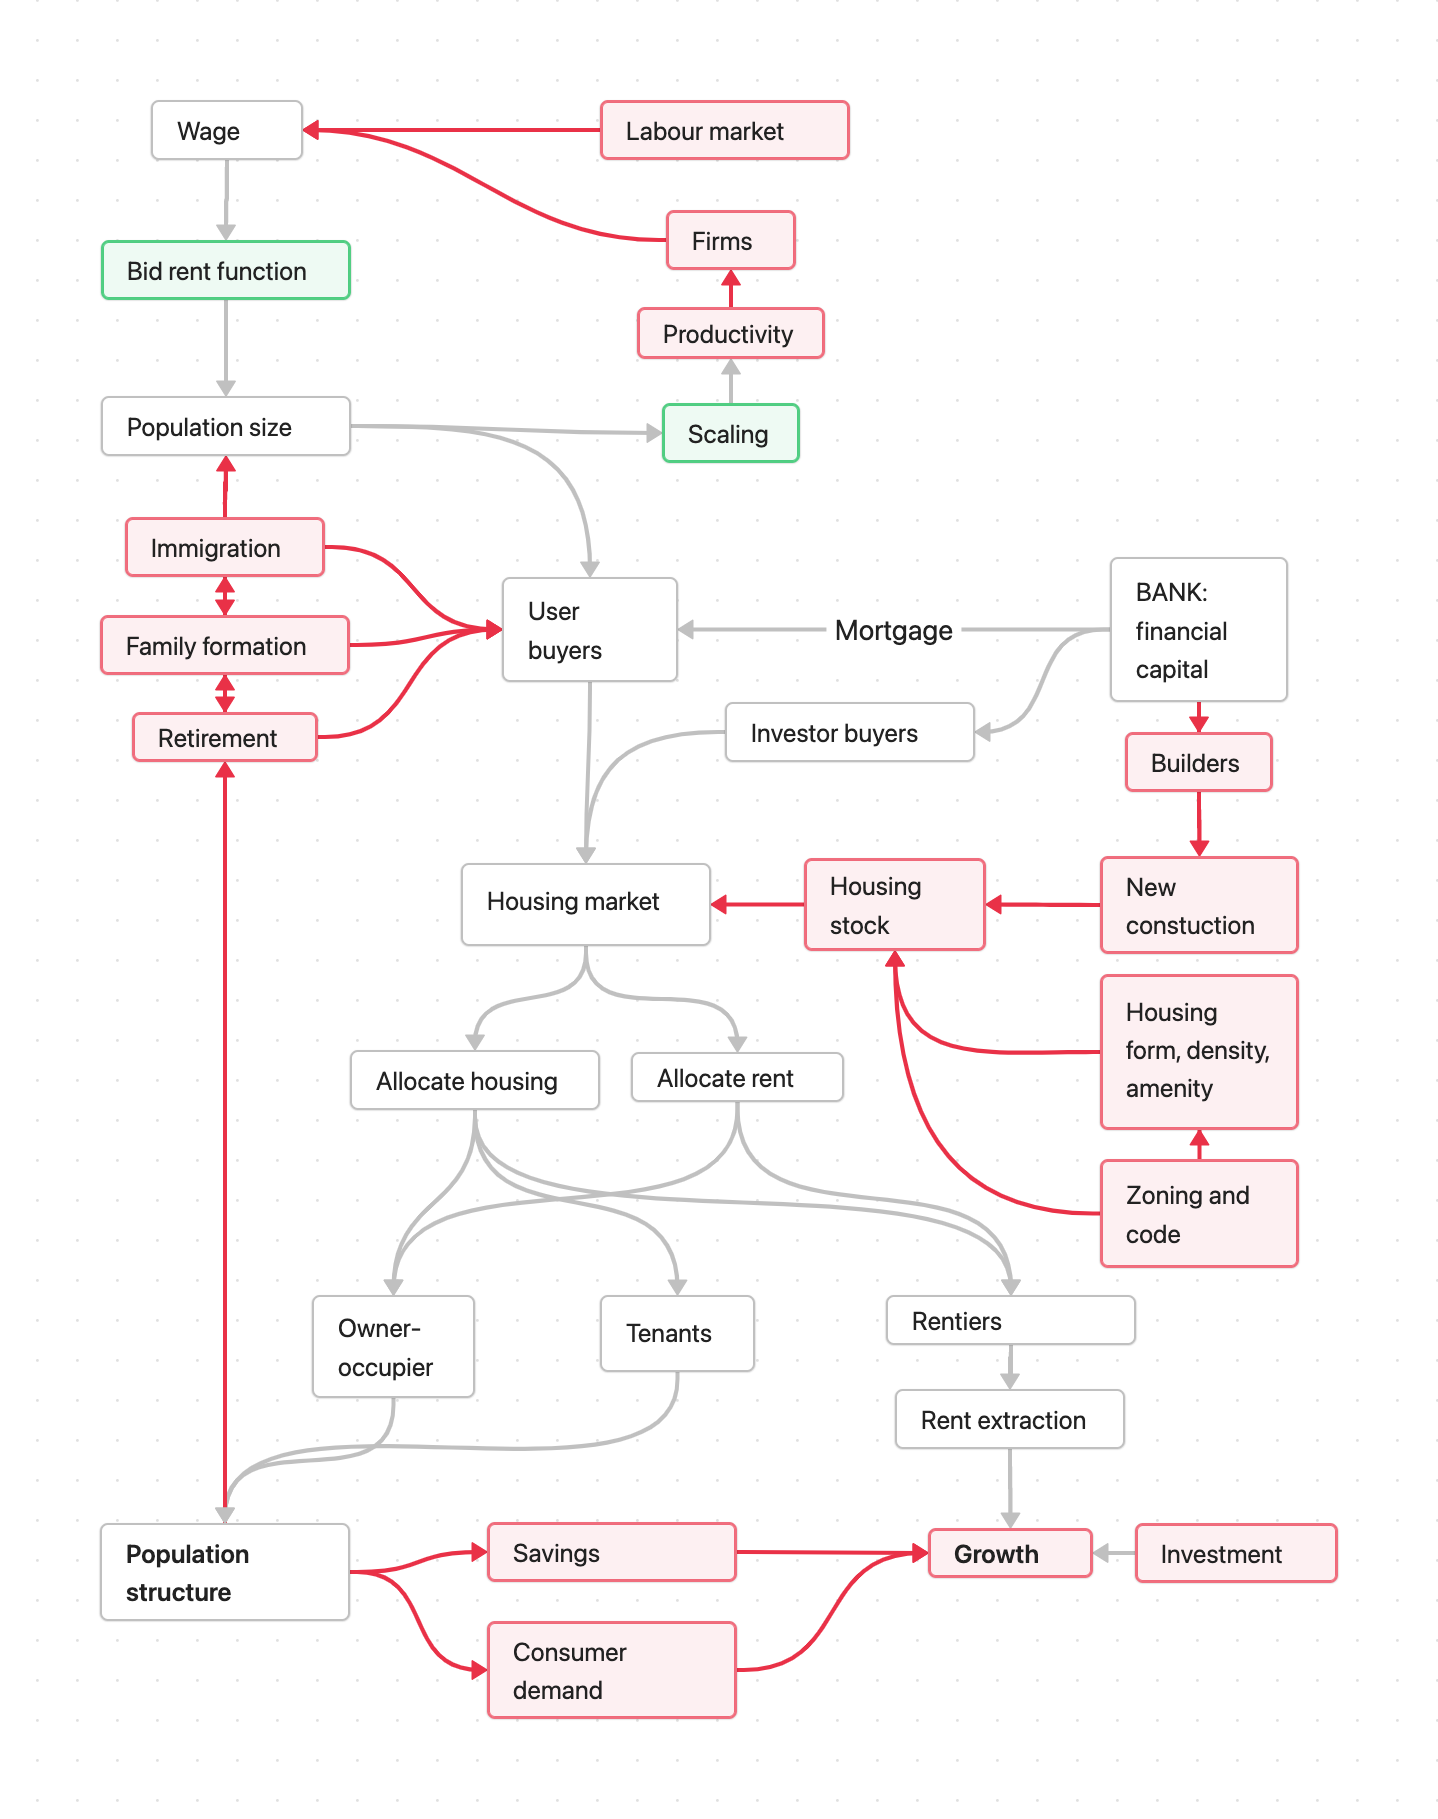
\includegraphics[scale=.22]{fig/extensions.png}
\end{adjustwidth}
\caption{Extensions}
\label{fig-logic-extensions}
%\pagestyle{headings}
% \usetikzlibrary{positioning}
%\begin{tikzpicture}[remember picture,overlay,shift={(current page.north east)}] \node[anchor=north east,xshift=-1cm,yshift=-1cm]{\includegraphics[width=1cm]{example-image-a}};\end{tikzpicture}

\end{figure}
}


At the bottom of the figure we introduce consumer demand linked to the population structure and feeding back to growth. Savings behaviour becomes more  complex when consumer demand is made endogenous and with as more complex population structure.

The fifth block of extensions illustrated in Figure~\ref{fig-logic-extensions} would replace the simple, scaling-based transmission mechanism in the Alonzo-Jacobs cycle with explicit firm and labour market behaviour. This class of extensions is obviously linked to population structure. It leads to consideration of firms that produce different products, some for export some for the local market, and to multiple types of labour.

Linked to the labour market and production system is the possibility of introducing competing cities. 

It should be clear that each of the extensions we suggest is potentially as complex as our core model, and each brings with it a collection of additional assumptions. We would argue that none of them would change our qualitative results greatly, although each would deepen our understanding of mechanisms and of the detailed impacts.


\section{Population pressure } 
Our basic model does not have a growing population. This conveniently allows us to isolate certain effects of financialization. Population pressure is one of the drivers of financialization because it amplifies speculative gains, however. As a result, one of the first extensions must be  to introduce population pressure.

There are two sources to consider: 
\begin{enumerate}
\item agglomeration effects that increase the wage and attract workers faster than the housing stock can respond. 

Worker agents from outside the city can always consider moving and accepting a job. 
% QUESTION - how to manage the flow of new agents?
%, or can make more from rents and moving away
\item immigration pressure
\end{enumerate}
under the  first, agglomeration economies drive population while under the second, population growth may drive agglomeration.

The growth of the housing stock will generally lag population growth, generating price effects and stock dynamics.

Agents will respond to increases in demand conditions. The perception that the market is tight or that prices are rising may lead to higher bids and reservation prices and shift results in favour of sellers.  


%Buyers could consider neighbourhood pressures, demographic changes, changes in job location, desire for amenity etc. in their assessment of housing need. 

%With multiple bids agents can place the most competitive bids on those homes they prefer. If they have higher urgency they place strong bids on more homes. 

%Next buyers request a selection of homes to consider from a real estate agent. Those with higher need for housing look at more homes. The real estate agent offers a selection of homes based on the agent's requirements. A randomness parameter determines how many divergent houses are also considered. When the parameter is 1, the selection of homes is fully randomized, When it is 0, the agent sorts all available homes and offers those which fit the agents budget, space, and other requirements best.


\subsection{Retirement investors and private investment properties}
The simple population turnover in our model can be replaced with a more complex set of possibilities at the agent level.  At retirement,  agents can be allowed to may choose between selling their home, renting it as an income property, or if there is sufficient amenity value for them, staying in the city. Implementing these choices complicates the agent decision and the resulting housing distribution but require few changes to the rest of the model.

\section{Housing production}

\section{Differences in density, housing form, and neighbourhood amenity}
Much of what is interesting in a city is the rich variety of housing forms and neighbourhoods and the varied populations that occupy them. Our model has a single form of housing and an undifferentiated populations, allowing us to differentiate the housing system in specific ways and study the interactions between the built world and the population. We are convinced that few of the possible extensions could affect our qualitative results. 

Nonetheless, in our agent based model, in which every lot is  addressable, it is simple to introduce zoning boundaries, local amenities, different densities or housing qualities and homes of different sizes. Hundreds of experiments are possible exploiting  the extensibility we have carefully conserved.  

We can ask what would be the effect of a hard zoning boundary and what would be the effect of suddenly relaxing it. We could explore the effect of speeding the rate of conversions from one size  home to another, or of locating high density pocket on a transportation route. Many significant urban policy questions could be examined with a limited amount of additional programming. 

\section{The consumer city}
Much of the demand for what is produced in the city is local consumer demand.  Our model has assumed there is production only for a perfectly elastic export demand. Consumer needs are buried in the subsistence wage. 

A minimal extension would be to introduce a second sector representing local consumption demand. A share of locally generated income would support production for the city's population. The labour force would be split between the two sectors and both productivity and wages might differ across sectors. 

A more complex treatment would introduce a range of service, entertainment and retail producers. This might be done monopolistically competitive firms \'a la Dixit and Stiglitz \cite{AvinashK.Dixit1977MCaO}.



\subsection{Distribution of rents}
Rents go to landowners, with a share taken for maintenance and taxes.
Rents may also be taxed, could be shared between multiple owners, etc.
 %\note{REPHRASE? rent is  extracted from the coalition of capital and workers.} % Rents may also be taxed, could be shared between multiple owners, etc. 
%The rents are captured by landowners.  The capture of rents by landowners is common buy not necessary. 
In principle the gains from urban productivity and amenity can be allocated as social wealth through shared ownership, as is often done on a small scale with cooperatives and land trusts, distributed to all citizens through something like a social wealth fund, or captured in taxes or fees as Henry George suggested. 
%The rents would otherwise go to labour and capital.





\subsection{Urban Savings - Contributions?}
THIS IS A CONTRIBUTION, BUT ALSO A DISCUSSION OF ONE WAY THIS WORK COULD BE EXTENDED, MIXED WITH A BIT OF MODEL DESCRIPTION

Conventional growth models specify a savings/investment mechanism at the national level. To our knowledge, this has not been done for the city level. We require  savings at two levels. First, since we want to incorporate  households home ownership and a relationship to the financial sector through mortgages, We specify a savings rate out of the spending we have isolated in the `subsistence wage' This means that both urban and rural workers accumulate savings, that savings are age-dependent, making the size of mortgage available also age dependent. 

Homeowners in addition have equity $E=P-M$ in their homes.  ({\color{red}Should newcomers also have equity? or is it built into the savings. Clarify this.} 

A second level of saving is the  investment in capital out of the city surplus. Even raising this question puts us into terra incognita. There are many  channels through which surplus flows into productive investment in the urban contest. One is through public investment in infrastructure. We have discussed how falling transportation costs increase surplus generation. Investments like this are made slowly and take effect over time periods much longer than our model is concerned with.  We can set a property tax rate   that we will assume is sufficient to maintain the stock of infrastructure.

Public and private investment in human capital is largely urban as well, but as with infrastructure, investment and response take effect over time periods much longer than our model is concerned with. 

Private sector innovation in technology, marketing, or products draws on local saving less but still significantly on local savings. We have little in the way of theory or empirical research on this channel. Lags between investment and any rise in the urban wage premium are almost certainly long and variable. 

We deal with this issue by linking local capital ownership with the scale factor. It is known that local ownership is associated with local investment. We will assume that local capital ownership, which consists in part of local ownership of the housing stock, can be proxied by homeowner equity as a share of local. 

\subsubsection{savings and retirement behaviour}
Agents fund their retirement from savings, as well as returns on their home if they have one to sell. Savings may be invested in a pension fund, or in local property,  depending on expected risks and returns. In the real world, financial institution manages most pensions, investing in the market or in property.  All this institutional structure is probably most easily handled by implementing a savings account for each agent. We are not interested in the detailed investment behavour for the financial sector.% either in the stock market, or in pensions.

%Institutional and individual investors can access debt. %

We could also consider a case where outside money can come under institutional management, not just local retirement savings. A parameter would control the inflow of additional money beyond local investment in the pension fund. 



\section{Making  labour market and firm behaviour explicit }
We have carefully developed the link between neoclassical growth theory and the literature on urban scaling \cite{bettencourtIntroductionUrbanScience2021} and  We then imposed the scaling result on our model.  We force the model to conform to the empirical data on the relationship between population and productivity. This amounts to black-boxing the entire production and labour demand sector as well as the construction and housing production sector. 

This made sense because our focus  was on the housing market and the financial sector, but the model we have constructed will allow us to ``fill the black box'' with more complete models of the production and labour market to see how they compare to the empirical data. 

The  scaling  literature also provides relationships between density and population and infrastructure cost and population that we can explore in the same way.

In the scaling literature, these relationships are increasingly theorized in terms of network effects, which is perfectly consistent with the Jacobs analysis and the more recent neoclassical growth modeling.


\subsection{The transmission puzzle}

The transmission of productivity increases arising from agglomeration effects  to the urban wage through firms, can be modelled in many ways. The agglomeration effects are external to the firm and therefore likely to be unexpected. If  firms underestimate the marginal product of labour, labour productivity will be greater than expected, output will be higher than planned output, and revenue and profits will therefore be higher than expected. Excess demand will attract more productive capital which in turn will demand more labour,  Rising labour demand drives up the wage. The agglomeration effect driving growth is essentially a public good in which individual firms will under-invest. This raises a policy challenge that we leave for others. CLARIFY - ALSO STILL A FOOTNOTE IN MODEL SECTION. CUT OR REF THEiR IF MOVING HERE.

 It is straightforward to compute the rate of excess return for  this model. 


\begin{figure}
    \centering
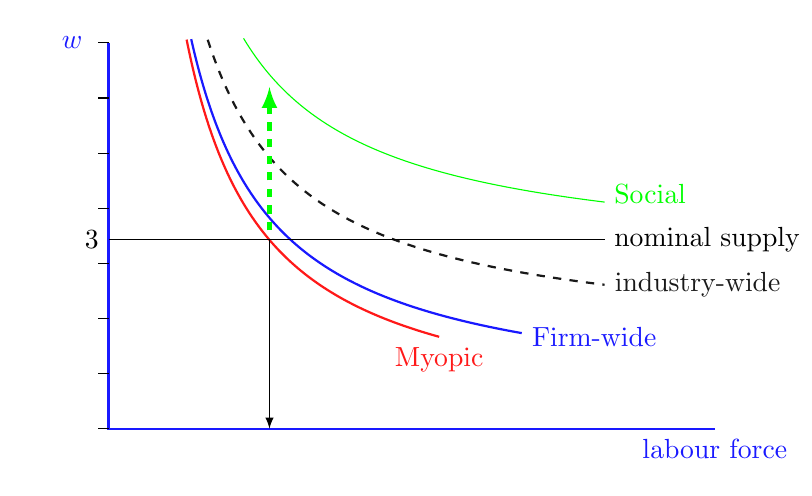
\begin{tikzpicture}[scale=.7]
%\def\bndmax{5}        %https://tex.stackexchange.com/questions/68462/filling-a-complex-region-with-tikz
%\def\bndmin{0.2}
\def \Y {7}  % height of y axis pecent
\def \W {15}  % length  of x axis
\def \Wbar {3} % jmeam wealth
\def \omega {3}
\def \A {1}  %was .5
\def \B {.5}

\draw [thick, color=blue!90] (0,\Y)node[left=.2cm]{$w$} -- (0,0)--(\W-4,0)node[below]{labour force};  
 \foreach \yi in {0,...,\Y} \draw (0,\yi)--(-.2,\yi)node[left]{};
 
\tikzset{func/.style={thick,  color=blue!90}}
% \draw[ func, domain=.2:\W-6] plot [samples=200] (\x, 2*\x^.5)node[below=.1, right]{SUPPLY};

\tikzset{func/.style={  color=green}}	
\draw[func, domain=2.45:\W-6] plot [samples=200] (\x, 10/\x+3)node[above=.1, right]{Social};

\tikzset{func/.style={thick, dashed, color=black!90}}	
\draw[func,domain=1.8:\W-6] plot [samples=200] (\x, 10/\x+1.5)node[ right]{industry-wide };

\tikzset{func/.style={thick, color=blue!90}}	
\draw[func,domain=1.5:\W-7.5] plot [samples=200] (\x, 10/\x+.4)node[below=.05, right]{Firm-wide};

\tikzset{func/.style={thick,color=red!90}}	
\draw[func,domain=8.5/6:\W-9] plot [samples=200] (\x, 10/\x)node[below]{Myopic};

\draw[](0,3.425)node[left]{$\omega$}--(9,3.425)node[right]{nominal supply };
\draw[thin,latex-](2.92,0)--(2.92,3.425); %a vertical labour supply
\draw[ultra thick,dashed, green,-latex](2.92,3.6)--(2.92,6.2);
%\draw [blue,  thick](13, 8.3)--(15,8.3)node [right, black] {\small A=\ 1,\ B=0.5};
%\draw [green, thick](13, 7.6)--(15,7.6)node [right, black] {\small A=.8, B=0.8};

%\node at (5,-1.5){Resulting in  profits, expansion, and/or entry: the city grows};
 \end{tikzpicture}
\caption{Multiple marginal products.}
\label{fig-marginal-products}
\end{figure}



Figure~\ref{fig-marginal-products} illustrates the problem. We can  make a distinction between the myopic marginal productivity curve observed by at the shop floor level and  the firm-wide effect of adding a worker. The red curve labeled ``Myopic'' represents the declining direct marginal productivity of labour as in might be observed by a shop manager, who could report how much more output one with one worker one lathe would produce. The blue line above it labeled ``Firm-wide'' represents the actual effect on firm productivity that arises because the new worker makes other workers in the firm more productive. This addition to output would be observable for managers reviewing the firm's performance over time. ' 

We can go on to consider the slower and distributed effect on closely related firms, which would raise any estimate of marginal product.  If there are 10 other firms and a new worker  has a small spillover effect  $\epsilon$ on each,  the spillovers raise the industry  marginal product  by $10\epsilon$. Each of the  10 other firms  enjoys  an additional $10\epsilon$ gain in the marginal product of their workers. This should lead to additional hiring by other firms.

Finally, expanding our view another step, we notice that if each of the  10 other firms hires one worker who produces an additional  $10\epsilon$ gain in output for all firms, the total spillover effect would rise by $100\epsilon$. The social marginal product of a single hire is indicated by the green line. 



\section{The system of cities}
Modern cities are not lonely and autarkic  beasts wandering their own exclusive territory and unconnected to others of the species. They are one is a global system of cities that compete and complement each other. Information, capital and even labour flows between cities are large. Henderson Abdel-Rahman\cite{Henderson1972Sizes}, Abdel-Rahman \cite{abdel-rahmanAgglomerationEconomiesTypes1990}, Fujita \cite{fujitaMonopolisticCompetitionModel1988}, Fujita, Krugman, and Venables \cite{fujitaSpatialEconomyCities1999}, and Fujita and Thiess \cite{fujitaEconomicsAgglomeration1996} among others provide models for expandingh the model in this direction.



\subsection{Taxes, municipal government, public goods, and productivity,}
This is a major issue with considerable development in the economics literature. Property taxes reduce the net locational value that flows to an individual owner but provides services and wages that make the city attractive. 

(create a regime where particular groups have an advantage)

Localized tax advantages can move a share of financialised investment into private consolidation of land.
including the structure of taxes for investment properties, institutional investors, individuals, etc.




\section{TO  METHODOLOGY?: Distribution}% not the right word
ABMs can be run multiple times to produce distributions of expected outcomes, which makes them valuable in planning exercises. They also do not require that we use a representative agent to make them tractable. Our model is intended to be elaborated  for such use. 

extensions
what it is
why it would be great to model
why it doesn't matter for our core results

\section{A possible typology of models and experiments}
While there  are many variations on the basic urban model and many potential experiments with each model there are only a few of immediate interest if the goal is to text the ``resilience'' of equilibria.

These models may exhibit irreversibilities in variables such as distribution, homelessness, city form, and class structure. 

The basic strategy for examining the system resilience is to shock a model (experiment) and then see if diagnostic variables recover. (This needs more precise expression.)

The first task is to select a subset of models an experiments that are of particular interests with respect to.

The second is to construct a model that allows those case to be examined. Ideally the model would be easily adapted to other experiments.

The following is a an attempt to develop a typology with a clear progressive structure.

Feedback - wealth allows upgrading. This advantages the rich. Maybe this 

\subsection{Models}
\begin{enumerate}
\item \textbf{A: The basic model}

The workhorse of urban economics is the circular city model. Some feature of the central place generates rents. It may be that it is the only employment centre. It may be economies of scale to a single activity or synergies arising from various externalities\footnote{We are interested in agglomeration economies. The wage  structure would then be related to the population or industry  structure. Externalities driving agglomeration may be classified  into two types, the  or so-called ``Marshalian''  and ``Jacobs'' externalities.}. 

In the simplest model, the central place pays a uniform wage, $w$ to all employees, who have identical preferences and transportation costs. $w$ is an attribute of individual residents. Residents  purchase or rent equal quantities of land at differing locations $l$ for identical housing.  

There are transportation costs $T$ that depend on distance from the  central place, so land close to the central place is more attractive than land farther from the central place.  

The equilibrium concept is that a market with identical individuals with identical incomes and transportation costs will result in identical utilities. The result is that land rent must decline with distance from the central place to offset rising transportation cost. 

The size of the city is determined by population and lot size. Income and transportation costs will interact with lot size. The basic model can be initialized by matching the number of properties to the size of the population. 

If population exceeds the number of properties there are three margins to consider
	\begin{enumerate}
		\item The land supply can increase. There may be a conversion cost
		\item The land per-capita may decrease. This is not simple in a city with land-use regulations, zoning, and fixed capital in homes. A conversion process has to be defined
		\item A homeless population can emerge. 
	\end{enumerate}

It is convenient in this model to use a \gls{Cobb-Douglas} utility function that has the property that a fixed fraction of income is spent on housing.  We can start with the assumption that earnings are fixed for the lifetime at the one-period wage, $w$. Then total spending on housing is $\beta Y, \beta <1$ and $ Y=w$. Let the transportation cost for a specific location $l$ be $T(l)$. The  equilibrium price at that location will be $P(l)= \beta Y-T(l)$.

It is convenient but not necessary to assume that land outside of the residential limit is costless. It is common to assume a fixed price for agricultural land. 

There is no fixed boundary and the size of the city is determined by the utility that can be achieved in competing regions of competing

\item \textbf{Y: The basic model with Income Differences}
This will result in segregation by neighbourhood depending on income. 

Income can be purely earning, which requires a distribution of $w$ across agents. Income  might include investment income, which  a private rate of return and a distribution of assets across agents. \footnote{A more subtle model could allow individual wages to be linked to the agglomeration of other workers - say engineers. we can imagine a city that has centres of agglomeration by profession or by complementarity. Depending on the production function, this should emerge endogenously.}
\footnote{Sufficient investment income could lead individuals to locate in cheap properties at the edge of the city.  Income might also be invested in property affecting the quality of a unit. This would require incorporating unit quality in the attribute list for each property, and introducing a quality preference  in the attribute s of residents.}

\item \textbf{L: The basic model with Locational Preferences}
This will result in segregation by neighbourhood depending on preferences.

One version would be include distance to the edge of the city as an amenity in the utility function. Another would be to locate amenities within the city. These would lead to higher prices near amenities.

A natural variant would be to have earning depend on location. If there were several locations  a polycentric city would emerge.

\item \textbf{T: The basic model with varied transportation cost }
This will result in segregation by neighbourhood depending on income and Transportation costs. Experiments include cars for the rich and  transit. 

Diagnostics include change in total transportation cost and differential welfare effects.

\item \textbf{R: The basic model with a rent-own choice}
This may result in the emergence of classes. Agents must have the capacity to borrow to purchase. Attributes of the agents and must now include  net assets,  an available interest rate, and a permissible mortgage.

We imagine a banker setting the mortgage rates and size. This can be done at the beginning of each period for each agent. 

With no income differential we expect equal utiliites

\item \textbf{YR: The basic model with earnings (Y) differences and a rent-own choice}
This model is likely to generate diverging classes as income differentials permit some to capture land rents from others. This is highly likely if borrowing costs decline with income and asset ownership.

\item \textbf{L: The basic model with variable lot size}
This is achieved by making lot size a choice variable for households, in which case we will get a trade off between transportation cost and lot size and distance. Results for this model are known. Density  falls with distance from the centre. 

\item \textbf{YL: The basic model with earnings (Y) differences and variable lot size}
The wealthy choose larger homes and lots farther form the centre

\item \textbf{S: The basic model with constant lot size and variable density}
This is achieved by allowing stacking of housing units. Results for this model are not known. This introduces a step change in housing form, and emphasizes unit size.

This model should produce some interesting spatial patterns, especially if couples with the possibility of secondary central places.

\item \textbf{YS: The basic model with earnings (Y) differences, constant lot size and variable density}

This model should produce some interesting spatial patterns, especially if couples with the possibility of secondary central places.

\item \textbf{IR: The basic model with outside investors and rent-own}

\item \textbf{IYR: The basic model with outside investors, earnings differentials and rent-own choice} This model is of interest if borrowing costs decline with income and asset ownership.
\end{enumerate}
\subsection{Experiments}
There are various experiments of interest. You will have to pick key ones. It is not necessary to do all of them in every model. 

	\begin{enumerate}
		\item increase population
		\item increase wage
		\item add hard boundary (limit land)
		\item Introduce differential incomes
		\item Introduce differential access to capital
	\end{enumerate}

% \newcommand{\cred}{\cellcolor{red!30}}
% \begin{table}[htp]
% \caption{Potential experiments: \textbf{Pick some}}
% \begin{center}
% \begin{tabular}{|c|c|c|c|c|c|}\hline

%   &\multicolumn{5}{c|} {experiments}\\ \cline{2-6}
% Model  &1 &2  & 4 &4  & \\ \hline
%  A& \cred& \cred  &  \cred & \cred  & \cred  \\
%  Y& \cred   & \cred   & \cred   &\cred    &\cred   \\
%  T & \cred   & \cred   & \cred   &\cred    &\cred   \\
%  R & etc &  &  &  & \\
%  L &  &  &  &  & \\
%  S&  &  &  &  & \\
%  I &  &  &  &  & \\
%  YR &  &  &  &  & \\
%  IR &  &  &  &  & \\
%   IYR&  &  &  &  & \\\hline
% \end{tabular}
% \end{center}
% \label{default}
% \end{table}%

\chapter{Future work to SORT}
model development (experiments and extensions)
interventions
theoretical development
% The urban production sector pays a wage premium $w$
%This is a convenient simplification, not a necessary feature of the model. 

The rental value of land shapes the city spatially.  

\section{Experiments with this model}
Lots of simple extensions e.g. 2 cities with immigration, differentiated labour, products, market power, neighbourhood effects (see extensions map/typology), we focus on those elements central to seeing the structure of the resilience dynamics of the wealth/housing effect. Consider adding density, to look at how it interacts with agglomeration effects. (integrating with transportation effects is neat)

\subsection{Initial state}
Basic experiments has all homes owner occupied to start. Other initial tenure mixtures are easily modelled. WHY WE MIGHT WANT TO

The basic model can be initialized by matching the number of properties to the size of the population. 

In the simplest version, firms concentrate at the city centre. Workers are spread over space and pay transportation costs to commute.

The size of the city is determined by population and lot size. Income and transportation costs will interact with lot size. 

\subsection{Parameter values}

\subsection{Analysis methods}
mapping of regimes

\subsection{Data}
incorporation of local data more carefully

\section{Extensions to the model}
The simple circular city can be extended to to produce other forms, including polycentric cities and hierarchies of cities at the cost of additional computational complexity. The simple case we examine will allows us to focus on the general, and neglected, distributional features of this class of models.

\subsection{Lags and adjustment processes}
The details of the adjustment process and the system lags are selected primarily for convenience in simulations. Real-time lags are important and complex, we explore some sensitivity results, but can explore more. 

We model a fairly short lag although in reality lags are long and variable. 

\subsection{Labour adjustment costs}

in the agent model, employees are simply laid off and seek work, so there is unemployment, but there are not \glspl{labour adjustment cost} for firms.

\subsection{Agglomeration effects, and returns to scale}
The case where there are increasing returns at the city level introduces interesting dynamics, explored in appendix CITE % 'furthur discussion' appendix.

We incorporate agglomeration effects using a Cobb Douglas formulation. This allows us to focus on the results of agglomeration in the urban system, rather than specifying the system of firms that transmit the effect. 
There are a number of other ways to study the aglomeration process in more or less explicit ways.

MOVE TO PARAMETER VALUE DISCUSSION?
The strength of the agglomeration is given by $\gamma$, thus for $\gamma=0$ there are not agglomeration effects. APPENDIX?
By definition, with one person, the agglomeration effect has no influence, $\Lambda(1)=1$,  as in the \gls{Cobb-Douglas}, and empirical urban scaling results tell us that agglomeration increases with population, following a power law distribution, so we know %$\die
FIX EQN ERROR die ${\Lambda}{n}>0$. 
%%%%%%%%%. ***WHY
If $\beta=1-\alpha$, this is a \gls{constant returns to scale} production function. Without agglomeration effects, $T(n)=1$,  Then  \textbf{$\mathbf{L(n) = T(n) n}$}  WHAT IS T, WHAT IS THIS TELLING US?
Without agglomeration effects, $\Lambda(n)=1$,  Then  \textbf{$\mathbf{L(n) = T(n) n}$} 


\subsection{Returns to scale and firm under-investment}
Each firm has \gls{decreasing returns to scale}, which means each new worker increases output by less than the previous worker did.
RETURNS TO FIRM CAN BE DECLINING WHILE RETURNS TO CITY INCREASING, THEN FIRM UNDER INVESTS
explore this in the model, see Equation~\ref{eqn-prod1}.

\begin{equation}
Y=K_i^{\alpha }(\Lambda(n)n_i)^{\beta }.
% \label{eqn-prod1}
\end{equation}

MOVE DISCUSSION HERE FOR NOW

\subsection{Heterogeneous agents}
In the simplest model, the central place pays a uniform wage premium, $w$ to all employees, who have identical preferences and transportation costs. 
The wage $w$ is an attribute of individual residents.  
It is straightforward to vary i and to vary preferences. 

relax assumptions and look at how the interaction between the production of social wealth in cities interacts with housing and the extraction of rent to drive patterns in a richer model with heterogenous agents interacting over space and time. 

- wages, skill sets

\subsection{Forward looking agents}
There are reasons to expect the results obtained with  forward-looking agents to differ substantially from those obtained with a model featuring myopic agents.\footnote{For example, Lecca et al. *** \cite{LOST-Lecca-et-al-2013}  used a stylized computational macroeconomic model applicable to a regional context to demonstrate that the assumption of myopic vs forward-looking agents yields differences in the dynamics generated by a shock perturbing the initial steady state, even though the alternative paths lead to the same long-run equilibrium.} 

\subsection{Rental bidding process}
 "Just as with prices, there is an economically \gls{warranted rent} which may differ from the \gls{market rent}. Individuals make their investment decisions on their own expectations rents. the bidding process on rental properties is abstracted in the base model. Instead of modelling the process explicitly, we make the assumption that the warranted rent is the market rent, $\mathcal{R}_W = \mathcal{R}_M$." .. could implement

\subsection{Amenity}
Notation for amenity.
There may be a band surrounding the city or persons who do not commute but enjoy urban consumption amenities. 
based on location etc

\subsection{Preferences}
A utility function/algorithm specifies agents preferences over the attributes that matter. - algorithmic continuous. lexicographic- any traits. 

\subsection{Unemployment and labour adjustment costs}
There is no unemployment. there are no labour adjustment costs for firms. ***INTERESTING TO THINK ABOUT  
when people would stop working with

 falls to subsistence wage -
 too much rent, I guess they leave, they can always move somewhere

\subsection{Moving costs}
     If there are moving costs, people can be trapped in a bad situation, incurring debt, and it can still be not worthwhile to move

\subsection{Mobility}
We could look at mobility in a more sophisticated way..
Agents enter the urban market two ways. If wages rise, agents just outside the city may become commuters. This increases population. 

When homeowners in the city retire they sell their home and move to the country. This allows them  to enjoy the capital value of their home.  They either sell their home or rent it to a new occupant. 

When  tenants in the city retire they would move to the country to enjoy lower rents. This has no effect on population. It is simplest, therefore to treat tenants as permanent residents unless we want the tenant's retirement to trigger an event like a rent increase or a decision by the owner to sell the property.

\subsection{Transportation costs}
Wage and transportation cost determine the radius of the circular city, which determines the size of the labour force which affects urban productivity. The cost of travel is therefore an important variable in the development of urban productivity. 

the transportation cost/distance relationship appears to be non-linear in many cases. While the linear model connects with the established literature, we likely want to explore the implications of more empirically grounded curve (e.g. \cite{bertaudSpatialDistributionPopulation2003}).

\subsection{Multiple firms and production structure}
The scaling result at the level of the city allows us to incorporate the effect of agglomeration in a standard \gls{circular city} model in a simple way. 

We could also explicitly model labour markets and competing firms. 

Explicitly modelling labour markets with multiple firms is a natural way to specify the model more completely, see Appendix~\ref{appendix-future-work},  but it would require introducing many ancillary assumptions and selecting among alternative models of agglomeration, when when we want to focus on distributional and growth-affecting features of the system.

For simplicity, assume firms produce a variety of perfectly substitutable commodities which are exported and locally consumed at a fixed price in a large market. 
***  Increasing product variety may produce a consumption agglomeration economies as in \cite{fujitaSpatialEconomyCities1999}.

\subsection{Market power and interchangeable goods - local markets etc}
MAKE A FOOTNOTE ON MARKET POWER AND INTERCHANGIBLE GOODS??
No externalities imperfect information etc.. ensure efficiency but aren't needed, all you need is price taking for individuals to only pay attention to their own costs and their own benefits. 

\gls{externalities}, \gls{imperfect information}, \gls{monopsony}, \gls{duopoly}, \gls{monopoly}

competitive markets many sellers, many buyers, monopoly single seller, monopsony - single buyer, intermediate cases - monopolistic competition - with some market power but not complete - duopoly- some inefficiency depending on the behavioural model because in the duopoly case they may be able to take advantage of the behaviour of buyers.

Start with perfect competition, then introduce monopolistic competition is most likely.. but it's more difficult to handle. e.g. with brand names, people have some preference for some feature of your particular good so you can price it higher even though you may loose some marginal people. Firms compete on brand name and reputation, not the pure cost effect.

In the spatial economy, goods are deferentially interchangeable. Put them on a line and firms pick a place along they line. Firms are in competition but are competing on a line-.. spatial model moved over to characteristic space..---looking at this would involve overlaying another space - the characteristic space on the physical space. .. There are also local places with local grocery stores. Polycentric stores have effectively monopolistic competition in real space. - like a named cafe downtown has the same.

\subsection{Sectors}
..


\subsection{Incomes}
In the model receive the\gls{urban wage}, which is the subsistence wage plus the urban wage premium $\psi + w$.

They may get different incomes because of firm, sector or individual increases, or particularities of the 
hiring/negotiation/wadge adjustment process, path dependency, stochasticity, etc. 
All of these factors could be explored formally in the model. %ref{rockefeller}


POOR STRUCTURALLY DISADVANTAGED HOWEVER RICH WE GET
these are averages-- some are structurally below average so some are always behind simply because of the structure of the rents claimed.. that's built in FUTURE WORK- DIFFERENT INCOMES GETS YOU THAT. 



\subsection{Hiring process and unemployment} \label{section-rockefeller}
 In our model, non-urban landowners are those who live too far from the urban job center to justify commuting.  Agents join the urban market by adding their names to the firm's list of job applicants when the rent on the marginal unit of land exceeds the transportation cost. 

adjustment speeds..
 
i(did extended modelling in the Rockefeller social innovation lab)- barriers of employment for young people seeking work
- prison records, transportation, family responsibility, bias, educational attainment, expectations of success, neighbourhood factors etc.
Could explore that kind of structure in this model

\subsection{Demographics}
Could build a population model suited to particualr data sets %\ref{section-rockefeller}

\subsection{Skills and individual productivity}
The basic model consideres a non-differentiated workforce. We can add particular skills.
Some agents can be more productive than one another

Agents may move to cities to assemble networks (model as networks)
and learn specialized skills

It can evolve over time so agents can productively over pay to  
-- getting debt/resources at key stages in a persons development to aquire property and skills is important to \gls{wealth trajectories}


\subsection{Sources of agglomeration effects}
Some of the empirically wage difference comes from the dense resources  - location of cities in good places, public investment- libraries - institutions, the network effects
some from the ability of those close to the center to simply claim a larger share of resources
some 
Some of the agglomeration wage may come from people with resources and skills disproportionately choosing cities for their amenity effect. 

We can explore different drivers in the model.


\subsection{TO METHODOLOGY: Rural market and other cities}

 To simplify analysis, we assume that land outside of the residential limit is costless, following th common practice of assuming a fixed price for agricultural land \cite{GET_fixed-price-ag-land}. 

The model is constructed so that there is neither land rent nor capitalist exploitation in the rural economy. 
This special case allows us to examine the distribution of the social surplus generated by agglomeration economies and the effect of financialization.

We could explore this

\section{Interventions: Policy and Agent Strategies}
Extended appropriately, this basic model could be used for planning.

detailed models of interventions typologies of interventions e.g. local currencies, decaying currencies, 

\subsubsection{Teaching}
could use for teaching a sequence for illustration could follow to introduce x ideas - see above. - rent, space, finance treated separately, - tool to think about their relation

productivity centered urban and spatial policy

connects with growth, economic development in real places work

\subsection{Zoning}
zoning - layers interact

\subsection{Taxes}
property taxes reduce the net locational value that flows to an owner but provides services and wages that make the city attractive. 

(create a regime where particular groups have an advantage)

Localized tax advantages can move a share of financilized investment into private consolidation of land.
including structure of taxes for investment properties, institutional investors, individuals, etc.


\subsection{Insurance, risk, and mortgage backing}

Uncertainty is a key variable.

The effects of policy are large. For example in Canada, backing mortgages is the largest fiscal investment at the national level \cite{nemtinFinancializationHousingSocial2021}.

- risks, bubbles, collapse


\subsection{Housing quality, size, subdivision}
Residents  purchase or rent equal quantities of land at differing locations %$l$ 
for identical housing.  DOWN

? More generally, if we were to introduce variations in lot size and housing types  we would want the integral of the worker density function. In our ABM version  of the model we simply count the workers within the commuter shed.

\subsection{Development and Improvements}
The supply of land at any distance from the center is inelastic. 
Its value comes from proximity to the productive urban centre, not from the value of improvements made to the property.

*** Without density, the labour supply increases with the square of the wage.  other forms..

- We have an empirical curve - gives density- simply build in

- We can .. Model a subdivision process-- urban SIM, a collaborator on the missing middle grant. - model of pro-forma and typoloties/ policies makes it possible to follow..

Some nonlinearities e.g. Some may buy land seeking to develop property in the future and let it become run down. 

We could add improvements
 or consolidation, subdivision, and development. 

% Reference sections on development which is different, and the contribution of amenity % Because supply is fixed for urban land, and the landowner has a monopoly claim on rents, the rents that can be depend on wages and amenity rather than the cost of improvements made to the property.
% The source of rents is the free gifts of nature, the coming together of people to create value in cities, and the concentration of public amenity in cities. 

\section{Theory - how to pay for innovation?}

Leaving land out, however, creates a problem in  the neoclassical growth theories we will examine below. John B. Davis \cite{davisRicardoTheoryProfit1993} noted that ``Questions arise, however, when one turns to exchange between a sector paying rent and one not.'' 
Under the assumption of perfectly competitive goods and factors markets as well as marginal productivity pricing of capital and labour, neoclassical growth requires technical change to be generated outside the model because there are no resources left to innovate if both factors of production are paid their marginal product.\footnote{This follows from Euler's theorem: if, for a given level of technology $\bar A$ output Y is produced according to a \textbf{constant returns to scale} and twice continuously differentiable function of capital and labour $F(K, L, \bar A)$, Euler's theorem implies that $F_K K + F_L L=Y$, where $F_i$ is the marginal product of factor $i$. Payments to  capital and labour take up the entire national product and no resources are left to finance the production of technology-improving innovations. are paid their marginal product.} 
If, however, land is reintroduced, as it must be in an urban model, there must be rents and there is therefore a surplus available for innovation.
\footnote{An alternative and common approach is to assume imperfect competition, which may be based on increasing returns to scale, in which case firms with market power may achieve a surplus. ``Although seldom modeled outside the monopolistic competition framework, market incompleteness and imperfect competition are central to the new growth theories'' (Gilles Duranton, Growth and imperfect competition on factor markets: Increasing returns and distribution, European Economic Review, 44-2, 2000, 255-280), Similarly, Sjak Smulders and Theo van de Klundert conclude that ``Growth is higher in a more concentrated market provided that market power of firms is not too high,'' (Imperfect competition, concentration and growth with firm-specific R \& D, European Economic Review, 39-1, 1995,139-160).}



\section{SORT Rough Notes}
what does a speculative over investment.  in housing  do? - hollowed out store front

who carries what risks- banks vs individuals

subdivision and density

multiple cities,
linear cities

differential skills and wages,
work from home

details of typologies, transportation networks, etc

- make it available as a part for other models, use other models in this model


 

\subsection{Implications}
\subsubsection{Agglomeration driven under-investment}

% % \chapter[Model Implementation]{Model Implementation}
\label{appendix-model-implementation}

\section{Urban wage premium}

$\omega$ is the urban wage premium. It is a share of the urban agglomeration effect. 

I think of this as worker income, $\psi + \omega + r_prime*savings$ 

The wage income  $\psi + \omega$ part has to be related to the marginal productivity of workers. The urban output function from Lobo et al \cite{loboUrbanScalingProduction2013} is  
\begin{equation}Y=AN^\beta\label{LoboEqn2}\end{equation}

Where $\beta$  is the scaling exponent, with a value of,  for example, 1.13  \`a la 
Lobo. $A$ is called the ``scale factor.''\footnote{Much of the analysis assumes scale invariance of  $A$.}  The \textbf{total urban marginal productivity of a worker} is  
\[UMPL=\beta AN^{\beta-1}=\frac{\beta Y}{N} =\]
This is not the same as the \textbf{firm-level marginal productivity of a worker}. The worker total share in Lobo et al. is \[W= (1-\alpha)Y \] 
so the individual share, which should be the competitive wage, is
\[W= \frac{(1-\alpha)Y}{N} \] 
where $(1-\alpha)=0.8$ is a common estimate. If we assume that this sets the rural wage,$\phi$, then $\omega$ has to come out of the  urban surplus per worker,

\[surp= \frac{\beta -(1-\alpha)Y}{N} \] 

 so set a fraction $\lambda$ of the surplus a, and 
 \[\omega= \lambda\frac{\beta -(1-\alpha)Y}{N}= (1.13-.8) \frac{Y}{N} \] 

 Since capital expects 0.2 as its payment and labor 0.8, the surplus available to share has to be taken out of the 0.13. The easiest formulation then is probably 
 \[\omega= \lambda(\beta -1) \frac{Y}{N} =\lambda(\beta -1) \frac{AN^\beta}{N} \] 
 

$(\beta -1)$ is agglom and  $\lambda(\beta -1)$ is the workers' share of the surplus over and above the \gls{constant returns to scale} (CRS) case.   $\lambda(\beta -1)$ is 

\begin{lstlisting}
# Firm step function updates wage, omega
def step(self):
    prefactor  = self.model.prefactor
    agglom     = self.model.agglomeration_ratio
    population = self.model.agglomeration_population
    wage_share = self.model.wage_share  
    wage_premium = wage_share * (agglom-1) * prefactor * population**agglom # omega
    self.wage = wage_premium + self.model.psi
    # k thought # self.wage_premium = (wage_share * prefactor * population**agglom)/ population # omega    
    # note surplus is: (beta - 1) * (prefactor * population**agglom)
\end{lstlisting}

Where wage share is a parameter input to the model.

\section{Bidding}
\subsection{Subjective discounting}
\begin{lstlisting}
def get_discounting(self):
    """
    Delta is the subjective individual discount factor for agent
    after one year. This will be close to ri
    A factor may be a compounded rate.
    It is the present value of one dollar in one year 
    Turns one dollar in one period into dollars of present value.
    sum_delta is sum of the infinite series 
    minus discounted infinite series after mortgage_period years
    It is the present value of annual payments from one to 
    mortgage_period years e.g. of mortgage payments or rent received
    delta_mortgage_period was called   delta_period_T
    """
    
    delta = self.r_prime # if constant 
    delta_period_1 = 1 / (1 + delta) 
    delta_mortgage_period = delta_period_1**self.mortgage_period
    sum_delta = delta_mortgage_period * (1 - delta_mortgage_period)
    # Note delta_mortgage_period is subtracted to subtract the long tail
    return sum_delta
\end{lstlisting}

Delta could also depend on wealth. For example,  use the bank rate, which is the rational rate but people who are poor typically have higher rates.  It would not change as the central bank changes r-pirme
% delta could be wealth based typically higher for poor.

\begin{lstlisting}
# A version with delta depending on wealth
wealth = self.wealth
delta =
\end{lstlisting}
 
\subsection{Maintenance costs}
\begin{lstlisting}
    def get_maintenance(self):
        """Maintenance share of property service (a*b*psi summed and discounted)
        OR IS IT TOTAL maintenance COST OVER THE MORTGAGE PERIOD?
        """
        a   = self.housing_services_share
        b   = self.maintenance_share
        psi = self.subsistence_wage
        sum_delta = self.sum_delta # CALCULATE PER PERSON
        return (a * b * psi) * sum_delta
\end{lstlisting}

\subsection{Taxes}
\begin{lstlisting}
    def get_tax(self):
        """ 
        THIS DOES NOT CHANGE WITH INCREASING WAGES?
        BUT THAT IS THE MAIN WAY TO FUND A CITY

        WHAT TO CALL THIS WEHRE DOES IT GO. WHERE DO WE USE THIS VS TAU
        Just for initialization? - warranted price. 
        Use warranted prices as initialization
        Tax costs for the mortgage period, T. 
        (Example of rate for an  multiperiod annual rate)
        tax_T= tau*(omega-c*d + a*psi) * sum_delta_T
        This is assuming taxes are paid at the end of each year for T years
        tau_T       = tau * sum_T_delta 
        #  present value of the tax rate over T years        
        """
        tau   = self.model.property_tax_annually
        omega = self.firm.wage_premium # FIXED
        psi   = self.model.subsistence_wage
        a     = self.model.housing_services_share
        c     = self.model.transport_cost_per_dist # RENAME
        d     = self.distance_from_center
        sum_delta = self.model.sum_delta # TODO - make individual  - this would have to be average discounting - THIS TAKE SUM DELTA OUT - AND PUT WITH LARGER CALCULATION.. - CACLULATE FOR A PERSON/PROPERTY COMBINATION..
        return tau * (omega - c*d + a*psi) * sum_delta
\end{lstlisting}


\subsection{TODO Warranted price}
\begin{lstlisting}
@property
def warranted_price(self):
    # USELESS PLACEHOLDER - GET CALCULATION
    return self.model.firm.wage/(self.transport_cost + 1) 
\end{lstlisting}

\subsection{TODO Maximum mortgage calculation}

\textbf{wealth-based  mortgage maximum} 
 \[max\ m_i = 9-\left(\frac{W_i}{\bar W}\right)^{0.1} \]

% **Source**: Ch:model line 580, page 87.. I have done some fiddling Wealth $W_i = P-M+S.  for i - real estate agents estimated price wealth of a property owner as assessed by the bank

\textbf{income-based  mortgage maximum} of 

\[M^{max}_Yi = \frac{0.28*(\omega+w)}{r_i}\] It is the maximum the bank will let you pay.

\textbf{Combined  mortgage maximum}
\[ M_i^Y{max} = min \{9-\left(\frac{W_i}{\bar W}\right)^{0.1}P,  \frac{0.28*(\omega+w)}{r_i} \}\]

\begin{lstlisting}
# Max mortgage
wealth = property_value - mortgage + savings
mean_weath = sum(wealth)/number_of_people

def get_max_mortgage(self, applicant):
    max_mortgage =  ...
    
    return max_mortgage
\end{lstlisting}

% wealth = property_value + 
wealth $W_i = P_e-M+S$.  

- Also need mean wealth. $\bar W$ , which you have to calculate from the sums for property values total mortgages issued, and individual savings. The bank could keep these values
- Individual borrowing rate 
$r_i = (A + B \frac{\bar{W}}{W_i})\bar r=(.1 + B \frac{\bar{W}}{W_i})\bar r$.
The value .1 can be seen as the bank's share of the prime rate set by the Bank of Canada. this is an easy place to insert that value. We should discuss this detail. An alternative is
$r_i = (0 + B \frac{\bar{W}}{W_i})(\bar r_i+ bank\ margin)$.

- Maximum M  from wealth constraint = $(9-(W_i/\bar W)^{0.1}P$
  Check if $(W_i/\bar W)0.9P$ will work. 
- Maximum M  from income = $M^{max}_Yi = \frac{0.28*(\omega+w)}{r_i}$ 
% - Maximum M  $M= min(0.28*(omega+phi)/r_i,  0.8P$,  (9-(W_i/\bar W)^{0.1}P,  \frac{0.28*(\omega+w)}{r_i}   } $


 
\subsection{Net rent based on}
Tenant willing to pay, vs what it is worth for a company to buy a property.

\begin{lstlisting}
def get_net_rent(self, property):
    """Compute the rent for a land parcel, or what someone could afford
    to pay to live there. 

    Rent depends on the urban wage premium over and above the subsistence
    wage, and on transportation costs and the distance to the
    central business district. Applies with a single wage. Adjust for
    differential urban wages.

    :param property: the land parcel to get rent information for.
    """
    a     = self.model.housing_services_share
    b     = self.model.maintenance_share
    c     = self.model.transport_cost_per_dist # RENAME
    d     = property.distance_from_center 
    tau   = self.model.property_tax_annually 
    # property_tax_rate # IS THIS FOR THE MORTGAGE PERIOD
    psi   = self.model.subsistence_wage
    omega = self.model.workers_share
    return omega - c*d - a*psi - b*a*psi - tau*a*psi
    # urban_wage = self.model.firm.wage
\end{lstlisting}


\subsection{Net rent based on ..}

\begin{lstlisting}
def get_net_rent(self, property):
    """Compute the rent for a land parcel, or what someone could afford
    to pay to live there. 

    Rent depends on the urban wage premium over and above the subsistence
    wage, and on transportation costs and the distance to the
    central business district. Applies with a single wage. Adjust for
    differential urban wages.

    :param property: the land parcel to get rent information for.
    """
    a     = self.model.housing_services_share
    b     = self.model.maintenance_share
    c     = self.model.transport_cost_per_dist # RENAME
    d     = property.distance_from_center 
    tau   = self.model.property_tax_annually 
    # property_tax_rate # IS THIS FOR THE MORTGAGE PERIOD
    psi   = self.model.subsistence_wage
    omega = self.model.workers_share
    return omega - c*d - a*psi - b*a*psi - tau*a*psi
    # urban_wage = self.model.firm.wage
\end{lstlisting}

\subsection{Max Bid}

Calculate max desired bid for an agent
\begin{lstlisting}
    def get_max_bid(self, property, bidder):
        net_rent = self.get_net_rent(property)
        r        = self.model.r_prime   
        r_target = r + self.model.r_premium
        m        = 0.8 # TODO FIX - ADD WEALTH
        # I can't do delta_T. It reads as delta_transpose to me.
        sum_delta    = self.model.sum_delta 
        p_dot    = 0.01 # TODO - estimate rate of price change
        return net_rent/((1 - m)*r_target - sum_delta*(1 + p_dot - (1 + r)*m))
\end{lstlisting}

Agent will bid the min of the desired bid or the max allowed mortgage
\begin{lstlisting}
max_mortgage = self.bank.get_max_mortgage(self)
min_downpayment = self.bank.min_down_payment_share * max_mortgage
downpayment = min(min_downpayment, self.savings)
max_allowed_bid = max_mortgage + downpayment
for sale_property in (self.model.realtor.sale_listing):
    # max_bid = self.bank.get_max_bid(sale_property, self)
    # TODO Fix
    max_desired_bid = self.model.bank.get_max_bid(sale_property, self)
    max_bid = min(max_allowed_bid, max_desired_bid)
\end{lstlisting}

\section{Negotiation Process}

Bidding.

There is a problem in that they bid on all properties as a short cut. If the number of bids structures the negotiation process, we need to limit their bids or do something much more iterative. (see above section)




\section{Individual Accounting}

\begin{lstlisting}
# FIX - NEED TO ADD THIS
# Update savings
self.savings += self.model.savings_per_step

# TODO pay costs for any properties owned
# if self.residence in self.properties_owned:
#     # TODO pay mortgage if needed pay costs
#     pass
# else:
#     self.savings -= self.rent # TODO check this is right rent
\end{lstlisting}
% \chapter[Parameters]{Computing Bid Price Parameters}
\label{AppendixParemeters}

% \section{Relating the bid price parameters to the code}
The bid price is: 
\begin{align}
P^{bid} \ge   \frac{ \mathcal{R}_N}{(1-m)r^{target}-\left[ \delta(1+L(P)- (1+r)m)\right]}. \nonumber
\end{align}
In the following sections, we discuss each of the terms and how they are implemented in the code. Sections are numbered: 
\begin{align}
\frac{\ref{SS:NetRent}} {(1-\ref{SS:BorrowingRatio})\ref{SS:targetr}-
\left[ \ref{SS:discountfactor}(1+\ref{SS:PriceForecast}- (1+\ref{SS:BankRate})\ref{SS:YWealthConstraint})\right]} \nonumber
\end{align}

\section{Net rent}\label{SS:NetRent}

$\mathcal{R}_N = \phi \mathcal{R}$


Where the \gls{rent share}, phi is a fraction
$\phi = (rent-taxes-costs) /rent$ 

There's a distinction between the warranted rent, the net rent, and the rent that's actually charged.



We assume that the  rent  actually charged to a tenant is the warranted economic rent, ($\mathcal{R}= \omega - \tau d_j$), but the relevant term to enter into the calculation of return on investment is the net rent $\mathcal{R}_N$ for a given property, because the returns are the returns an investor can get after paying taxes and operating costs.

In our computational model, we do the calculation in terms of a mortgage, so we want the total returns after expenses, in present value, compounded over the mortgage  period.
% We want the total returns after expenses, in present value, compounded over a 5 year period.


\begin{align}
\mathcal{R}_N &= \mathcal{R} - \Theta - \Sigma 
\end{align}


In terms of the warranted rent, 
\begin{align}
\mathcal{R}_N &= (1-\kappa_j - \sigma_j)(\omega - \tau d_j)
\end{align}

% $\mathcal{R}_N = (1-\kappa_j - \sigma_j) (\omega - \tau d_j)$

% {\color{red}
% Notice that  we need here is really the fraction of the warranted rent that the owner gets to keep after maintenance costs and taxes. It is possible that the owner is charging more or less than the economic  rent, but economic rent can be seen as an equilibrium value. Economic rent is $\mathcal{R}$.  This is (tautologically) related to the price as a fraction of the actual sale price: COULD MOVE TO THE CHAPTER NOW SINCE THE THE SECTION IS MOVED THER
% }

% \[\mathcal{R}= \frac{\mathcal{R}}{P_0}P_0 \]



If we want to know the  present value  of the \textbf{net rent}, $\mathcal{R}_N$  collect over the period  $T$, $\mathcal{R}_N^T$, we \textbf{add up} the discounted rents for each year. We may assume the rents are rising at and that the first is the current warranted rent, which gives us a computational formula. 
\[\mathcal{R}_N^T= (\omega-\tau*d)\sum_{t=0}^{t=T-1} \frac{(1+\dot{\mathcal{R}})^{t}} {(1+r_{r_\delta})^{t+1}} \]


% \[\mathcal{R}_Nj^T= (\omega-\tau*d_j)\sum_{\tau=0}^{\tau=T-1}\left[\frac{1+\dot{\mathcal{R}}}{1+r_{r_\delta}}\right]^\tau \]
\noindent where $\dot{\mathcal{R}}$ is an expected rate of change of rents - possibly zero for now, and $r_\delta$ is the individual's discount rate. 

TODO: problem - how to handle subscripts with net rent $\mathcal{R}_N$



\subsection{Target interest rate}\label{SS:targetr}

 The target interest rate, $r^{target}$, is the prime rate plus a margin. % required by the bank.  Question: do non-bank actors have such a term?

\begin{verbatim}
self.get-target-interest-rate(buyer)
\end{verbatim}


\subsection{Tax ratio}\label{SS:taxratio} 
The tax ratio $\sigma$ is the share of rents that the municipality takes for services and infrastructure. This fraction of the value of the property is about 30\% based on mill rates in Ontario,  so $\sigma = 0.3$. % REFERENCE

*** CHECK Total taxes paid on  property $j$, over a given mortgage period $T$ is 

\[\Psi_j^T = \psi * \mathcal{R}\].  


\subsection{Cost tax ratio}\label{SS:costratio} 
The value of $\kappa$  varies for every property based on maintenance requirements, historic rents, tenant rights, and variations in assessed values. If it varies, it may be useful as a quality indicator.

%Values for $\kappa$ and $\sigma$ must be adjusted to take into account the length of the period or net rents have to be summed over the period.  NO LONGER NEEDED 

Nothing prevents $\sigma+\kappa >1$, which would leave an investor unable to cover building maintenance and taxes out of current rent. 


\subsection{Discount factor}\label{SS:discountfactor}

The discount factor $\delta_i$ for THE END OF period $T$ captures the cost of waiting $T$ periods to sell the property. The usual way to treat it, which we use here, is to assume that $i$ has an interest rate $r_i$ and has been investing efficiently. This means that  the individual has a discount factor for future returns based on the year-over-year rate of return. 

\[\delta^T_i=\left[\frac{1}{1+r_i}\right]^T\]


\subsection{Price forecast approximation} \label{SS:PriceForecast}
$L(p)$

$p$ is all the price data plus any exogenous information (EG Policy knowledge?). $L(p)$ is an estimation function that produces a `common knowledge' value for the rate of price increase. Later you can add idiosyncratic extra knowledge or extra ignorance.




\subsection{Prime interest rate}\label{SS:BankRate}
$r$

The bank's interest rate, $r$, is just the bank rate (prime rate? set by the Bank of Canada. Exogenous. Just assign  a value like 4\%.


\subsection{Borrowing ratio}\label{SS:BorrowingRatio}
$m_i$

The borrowing ratio, $m_i$, is just the fraction of the price that the bank will lend to a potential buyer. \textbf{It may depend on the individual.} 

Income(\ref{SS:YWealthConstraint}) and/or wealth (\ref {SS:MWealthConstraint}) may constrain individual participation in markets. 
Here we should use the same logic as we use about the interest rate charged. (\ref{SS:BorowingRate})


It is likely to be higher for institutional buyers  and for rich people because the bank thinks rich people are more secure risks. they may have other assets that could be attached in the case of default.

\subsection{Wealth constraint on m} \label{SS:MWealthConstraint}


I have suggested that the availability of  capital is known to differ for rich and poor. 
The bank, as a person has lots of assets, so $m_i$ is close to one, say 0.9. 

For the median wealth holder, $m_i$ should be around - let's say, 0.8 and  
We need a function that captures this relationship so we need to define individual wealth:
\[W_i= P_i -M_i  +S_i\]
where 

\begin{tabular}{ll}
$P_i$ & value of owned home\\
$M_i$ & Mortgage on owned home\\
$S_i$ & personal savings = $age*d*W$\\
\end{tabular}


We first tie the borrowing \textbf{ratio}, $m_i$,  for agent $i$, to individual wealth. Figure~\ref{Fig:Borrowingratio} illustrates a mortgage availability  model that is written 
 \[ m_i = 0.1(9-\left(\frac{W_i}{\bar W}\right)^{0.5}/2 )\]
Where $\bar{W}$ is mean wealth and $W_i$ is individual wealth. 

\begin{figure}[htb]
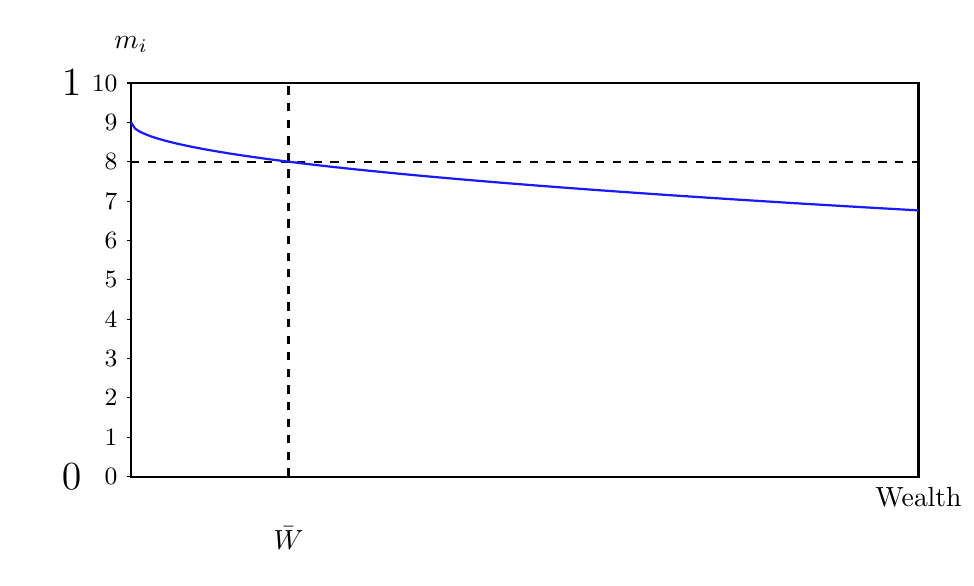
\begin{tikzpicture}[scale=.5]
%\def\bndmax{5}        %https://tex.stackexchange.com/questions/68462/filling-a-complex-region-with-tikz
%\def\bndmin{0.2}
\def\Y{10}  % height of y axis pecent
\def\W{20}  % length  of x axis
\def\Wbar{4}
\def\rbar{8}% this is the prime rate

% %Equation   \[ r_i = (A + .5 \frac{\bar{W}}{W_i})\omega\]
   % \def\Wmin{.63}  %This sets the lower limit fo the 
    \def\Wmin{(\B*\Wbar)/(\Y/\rbar-\A)} %function to keep in in bounds
	
 \tikzset{func/.style={thick,color=blue!90}}	

 \draw [thick](\W,\Y)-- (0,\Y)node[left=.5cm]{\Large$1$}node[above=.25cm]{$m_i$} -- (0,0)node[left=.5cm]{\Large$0$}--(\W,0)node[below]{Wealth}--cycle;  	% Axes box
 
 \draw [dashed, thick] (0,\rbar) -- (\W,\rbar);  	% Axes
\draw [thick,dashed] ( \Wbar,0)node[below=.5cm]{$\bar{W}$} -- (\Wbar,\Y);  	% Axes

\foreach \yi in {0,...,\Y} \draw (0,\yi)--(-.1,\yi)node[left]{\small$\yi$};
%\foreach \yi in {0,2,4,6,8,10} \draw (0,\yi)--(-.1,\yi));
%node[left]{\small$\yi$};
%\foreach \yi in {0,2,4,6,8,10}node at (-.1,yi) {{10*yi}} ;
\draw[func,domain=0:\W] plot [samples=200] (\x,(9-\x^.5/2);

 \end{tikzpicture}
\caption{Individual borrowing ratio $m_i$ as a function of wealth (in tenths)}
 \label{Fig:Borrowingratio}
\end{figure}


\subsection{Individualized borrowing rates}\label{SS:BorowingRate}
 $r_i$ 
 
 $r_i$ should depend on  both the person's income and their assets compared to others. The median after-tax income of Canadian families and unattached individuals was \$66,800 in 2020 according to Statistics Canada's \href{https://www150.statcan.gc.ca/n1/daily-quotidien/220323/dq220323a-eng.htm}{Canadian Income Survey, 2020}.  \href{https://www150.statcan.gc.ca/t1/tbl1/en/tv.action?pid=1110005501}{Data released in 2020 by Statistics Canada} indicates that the top 1\% of Canadians made, on average, around \$512,000 in a single year. \href{https://www150.statcan.gc.ca/n1/daily-quotidien/201222/dq201222b-eng.htm}{Survey of Financial Security, 2019}.

 A study by Statistics Canada found that the typical Canadian household now has a median net worth of \$329,900, while the average net worth in Canada is \$738,200. \href{https://www150.statcan.gc.ca/t1/tbl1/en/tv.action?pid=1110005501}{High income tax filers in Canada}

\subsection{Computing the income constraint on interest rates}\label{SS:YWealthConstraint}
$r_i$

In our model, we  tie the individual cost of capital,  $r_i$ for agent $i$, to a prime rate, $\bar r$ or the bank's target rate, $r^{target}$, prime plus 1\%, say. and to individual wealth. Figures~\ref{Fig:Borrowingrate1} and ref{Fig:Borrowingrate1} illustrate a couple of possible  cost-of-borrowing models roughly consistent  with the stylized facts about lenders. 

\begin{align}
 r_i =  &  \left(A + B \frac{\bar{W}}{W_i}\right) \bar r       \label{eq:incomeandr1}  \\
 r_i =  &  \left(\bar r - A + B *\frac{\bar W}{W_i - C}\right) \label{eq:incomeandr2}  \\
\end{align}
Where $\Bar{W}$ is mean wealth and $W_i$ is individual wealth. In Equation~\ref{eq:incomeandr2},  A determines y-shift, B, the scale, and C the  x-shift for the curve.


\begin{figure}
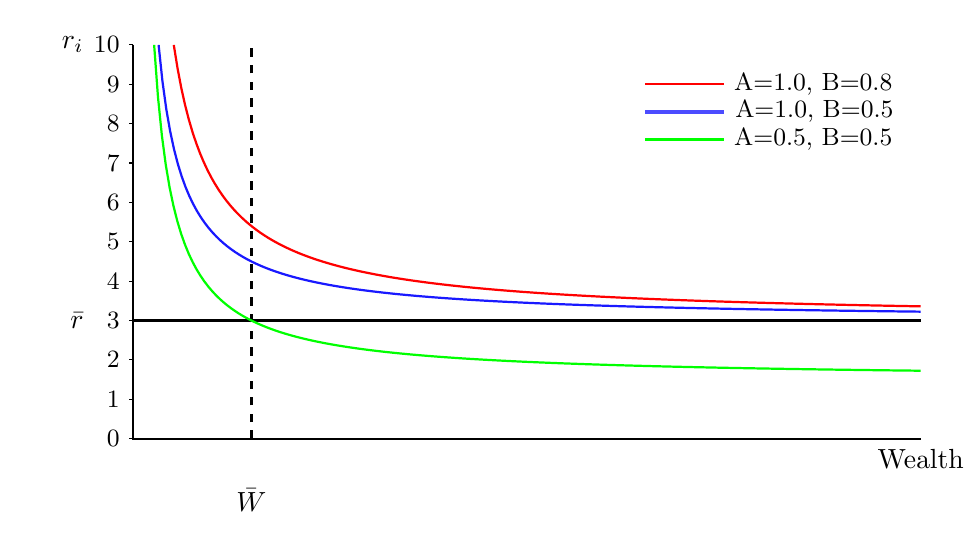
\begin{tikzpicture}[scale=.5]
%\def\bndmax{5} % https://tex.stackexchange.com/questions/68462/filling-a-complex-region-with-tikz
%\def\bndmin{0.2}
\def \Y {10}    % height of y axis as a pecent
\def \W {20}    % length  of x axis
\def \Wbar {3}  % mean wealth
\def \rbar {3}  % the prime rate 

% Equation   \[ r_i = (A + .5 \frac{\bar{W}}{W_i})\omega\]
\def \Wmin{.63}  %This sets the lower limit fo the 
\def \Wmin{(\B*\Wbar)/(\Y/\rbar-\A)} %function to keep in in bounds
\tikzset{func/.style={thick}}	

% Axes
\draw [thick] (0,\Y)node[left=.5cm]{$r_i$} -- (0,0)--(\W,0)node[below]{Wealth};  
\foreach \yi in {0,...,\Y} \draw (0,\yi)--(-.1,\yi)node[left]{\small$\yi$};
\draw [thick] (0,\rbar)node[left=.5cm]{$\bar r$} -- (\W,\rbar);  	% Axes
\draw [thick,dashed] ( \Wbar,0)node[below=.5cm]{$\bar{W}$} -- (\Wbar,\Y);  	% 

\def \A {1.0}  \def \B {0.5} %BLUE
\draw[func,domain=\Wmin:\W, color=blue!90] plot [samples=200] (\x,{(\A+\B*\Wbar/\x)*\rbar});
\draw [ultra thick, color=blue!70 ](13, 8.3)--(15,8.3)node [right, black] {\small A=\A,\ B=\B};

\def \A {0.5} 
\def \B {0.5} % GREEN
\draw[func,domain=\Wmin:\W, color=green] plot [samples=200] (\x,{(\A+\B*\Wbar/\x)*\rbar});
\draw [thick,  color=green](13, 7.6)--(15,7.6)node [right, black] {\small A=\A, B=\B};

\def \A {1.0}  \def \B {0.8} % RED
\draw[func,domain=\Wmin:\W, red] plot [samples=200] (\x,{(\A+\B*\Wbar/\x)*\rbar});
\draw [thick,  color=red](13, 9)--(15,9)node [right, black] {\small A=\A,\ B=\B};
% KEY
\end{tikzpicture}
\caption{Individual borrowing cost as a function of wealth}
\label{Fig:Borrowingrate1}
\end{figure}


\begin{figure}
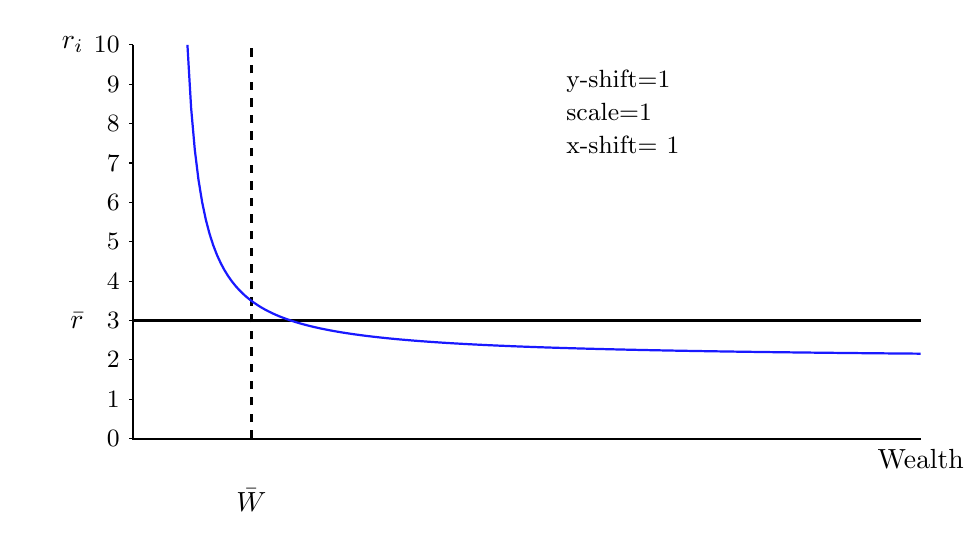
\begin{tikzpicture}[scale=.5]
%\def\bndmax{5}        %https://tex.stackexchange.com/questions/68462/filling-a-complex-region-with-tikz
%\def\bndmin{0.2}
\def \Y {10}  % height of y axis pecent
\def \W {20}  % length  of x axis
\def \Wbar {3} % meam wealth
\def \rbar {3}% this is the prime rate 

%\def \Wmin{(\B*\Wbar)/(\Y/\rbar-\A)} %function to keep in in bounds
\tikzset{func/.style={thick}}	
	% Axes
\draw [thick] (0,\Y)node[left=.5cm]{$r_i$} -- (0,0)--(\W,0)node[below]{Wealth};  
\foreach \yi in {0,...,\Y} \draw (0,\yi)--(-.1,\yi)node[left]{\small$\yi$};
\draw [thick] (0,\rbar)node[left=.5cm]{$\bar r$} -- (\W,\rbar);  	% Axes
\draw [thick,dashed] ( \Wbar,0)node[below=.5cm]{$\bar{W}$} -- (\Wbar,\Y);  	% 

\def \A {1} %vertical shift aroung \rbar, the prime rate
 \def \B {1}  % Scales the exponential curveBLUE
 \def \C {1}  %right shift  
% \def \Wmin {.4+\B}  %This sets the lower limit fo the 
\def \Wmin {(\B*\Wbar)/(\Y-\rbar+\A) +\C} %function to keep in in bounds

\draw[func,domain=\Wmin:\W, color=blue!90] plot [samples=200] (\x,{\rbar-\A+\B*\Wbar/(\x-\C))});
\node  [align=left, text width =2cm ] at (13, 8.3) {\small y-shift=\A \newline scale=\B \newline x-shift= \C};

 \end{tikzpicture}
\caption{Individual borrowing cost as a function of wealth II}
\label{Fig:Borrowingrate2}
\end{figure}

The rates $\delta,\ \sigma,$ and $r$ depend on the period, $T$. 

\section{Incorporating growth and discounting}
%We need a time period T for calculations. For use in any calculation, 

With a price-growth rate of $\dot P$ per year, the growth over $T$ years is $(1+\dot P)^T$, and  %and a 5 year mortgage period, 
the expected price at the end of the period is:

\[P^e_T=P_0(1+\dot P)^T\]

If, for example price growth is 10\%, $\dot P= 0.1$, the {capital gain}, or growth, over a 5-year mortgage term is 0.61051 $\approx$ 60\% of the original price, $P_0$.

If we want the compounded interest rate person $i$ the term T,
\[r_i^T=(1+r_i)^T\]
% This is the value we use in equation~\ref{EqBidPrice}.

If person $i$  discounts at a discount rate $r^\delta$, the present value of a receipt at time $t$ is calculated by using the \textbf{discount factor} $\delta_i^T$.

\[\delta_i^T= \left( \frac{1}{1+r_\delta} \right)^T \]
%\[\delta_i^T= \sum_{\tau=0}^{\tau=T}\left( \frac{1}{1+r_\delta} \right)^\tau \]
 
These can be combined into a function %\delta that  gives a single discounting factor  for a value  like future price that is both growing and being discounted over several (T) periods:
\[ PDV(P^e_T)=P_0\left( \frac{1+\dot P}{1+r_\delta} \right)^T \]
This PDV function specifically combines any expected rent increase, the individual's discount rate and the mortgage term into a single operation.

\subsection{Mortgage availability}
For home loans, many personal finance experts recommend total housing costs account for less than 28\% of your \textbf{gross} household income, This gives us an \textbf{income-based  mortgage maximum} of \[M^{max}_Yi = \frac{0.28*(\omega+w)}{r_i}\] It is the maximum the bank will let you pay.

We assume $r_i$ is based on the individual's assets, on relative wealth. Where is it calculated for the householder or the bank?

We get a \textbf{price-based mortgage maximum} \[M^{max}_P = 0.8P_0\] where $P_0$ is the actual sale price. This is based on the maximum amount of risk that the bank is willing to take on. ($P_0$  will not always be the same as the asking price or the warranted price.)


\section{Table}

\renewcommand{\arraystretch}{1.5}
\begin{tabular}{rlrr}\
Symbol         & Name                                 & Value      & Formula  \\ \hline
$m_i$          & Individual borrowing-ratio           & 0.75-0.85  & $M/P^{ask?}$ \\
$M^{max}_Yi$.  & Maximum mortgage based on income     &            & $\frac{0.28(\omega+w)}{r_i}$ \\
 $M^{max}_P$   & Maximum mortgage based on the price  &            & $0.8*P_0$ \\
$IS$           & Income share for housing debt        & 0.25-0.35  & Missing? \\
$\rho$         & Rent ratio                           &            & $\frac{\omega-tau*d_i}{P_0}$ \\
$\kappa $      & Operations ratio                     & 0.1-0.3    & e.g. $ 0.2\frac{\omega-tau*d_i}{P_0}$ \\
$\sigma$       & Tax ratio                            & 0.25-0.35  & e.g. $ 0.3\frac{\omega-tau*d_i}{P_0}$ \\
$\dot P $      & Price growth                         & []         & $\frac{P_t-P_{t-1}}{P_{t-1}}$\\
$P^T_e$        & Expected price in T years            &            & $P_0(1+\dot P)^T$ \\ % *** WAS $P^e_T$ 
$r_i^\delta$   & Individual discount rate             &            & To assign \\
$\bar r$       & Prime interest rate                  &            & \\
$r_i$          & Individual borrowing-rate            &            & \\
$r^{target}$   & Target interest rate                 &            & $\bar r + margin$ \\
$\delta_i$     & Discount factor for T                &            & $\left(\frac{1}{1+r_i^\delta}\right)^T$ \\
\end{tabular}
\renewcommand{\arraystretch}{1.0}


todo look for $P^e_T$ 

%==========================EXAMPLE=========================== https://www.kaggle.com/code/prateekmaj21/basic-financial-calculations-using-python/notebook
  
% def compound_interest(p,r,t):  %EXAMPLE
    
%     print('Amount: ', p)
%     print("Rate of Interest (Per Annum)", r)
%     print("Time (In Years): ",t)
    
%     a= p*((1+r/100)**t)
    
%     ci= a-p
%     print("Final Amount: ", a)
%     print("Compound Interest: ", ci)
 

\section{Transportation costs}
Transport costs have two parts:
1) fuel and vehicle costs per km
2) time costs per km

\subsection{Vehicle related costs}
Use one year as the wage period, converting transportation costs per km to annual cost for consideration in the household budget. Starting with the cost per km, calculate the cost per year:

\textbf{cost per km =$\textit{t}$}:. \$0.59   (from  Ontario data, 2021). sensitive to congestion, use of subways (\$5 /day?), 

 \textbf{work trips per year} 2 way * 5 days/week * 50 weeks work days = 500. [range: 450-550]

\textbf{cost per km-year} = work trips per year*cost per km

=\$0.59/km*500 trips/year  =  \$295/km year 



\subsection{Time costs}
\textbf{time per km}. range: 20km/hr -> 3min/km, 40km/hr -> (1.5min/km - 3min/ km)per trip 

(New York rush hour is much slower:  4-9km/hr ->6-15 min/km)

\textbf{time  per km-year} = work trips per year*time t per trip = 500* 3min  = 1500 min/km year = 25 hours= 3-3.5 days/km
 
\textbf{time cost per km-year} =  (days per km-year /work days/year)*wage premium per year  = 3/250 = 0.012 years/km year. ?

\textbf{money cost of time per km year} 

=time cost per km-year* wage(including subsistence) 

= 0.012 year* wage per year

\subsection{Total cost per km year of commuting for one agent}
\textbf{money cost of time per km year + \$295/km year * distance} \\
= (0.012 w+ \$295)/km year 
    \begin{quotation}
    \textbf{Example}
    To get a sense of the required wage if we have this annual cost structure, assume city\_extent $d^*$ is 30 km. At this point the transport cost is equal to the wage

\[(0.012 w+ \$295)/km year)*30 =  w\] 
\[.36w+ 8850=w\]
\[w=13828.12\]
        \begin{quotation}
        \textbf{PLAUSIBILITY CHECK}
This is plausible land rent, but does not include building rent. 
Capitalized at 5\% this house is worth \$ 276,562, a fairly cheap house 30 miles from city centre
        \end{quotation}
    \end{quotation}

{\color{red}
\subsection{? Value of $t$ to use in model}}
\[ \tau=(0.012 w+ \$295)/km year \]


% \chapter{Amenity}\label{chapter-amenity}

In this chapter, we discuss how amentity might be treated in this model. 
% from Ricardo_Rent_and_Roemer_3.tex
In our base model,  an urban wage premium is the only labour attractor. Transportation costs to the urban center determine land values. Effectively in our base model, we have set the level of amenities to zero  to focus on the productivity effects. The wage premium provides a reason to find housing in the city and to travel to the city centre to work. Housing choice, however, in reality is always the purchase of a bundle of characteristics such as location, building space, yard, local density and local \glsdisp{amenity}{amenities}. Stegman  found that ``a large majority of families who have recently moved to the suburbs are more concerned with neighborhood quality than with accessibility to other parts of the metropolitan region.'' 
``There is evidence that the amenities offered by a city enhance its growth'' \cite{clarkAmenitiesDriveUrban2002, falckPhantomOperaCultural2011} and that amenity effects themselves scale superlinearly \cite{kraemerCulturalSustainabilityUS2022}.

Kaufmann et all \cite{kaufmannScalingUrbanAmenities2022} investigated the general statistical patterns in the quantity and spatial distribution of different urban amenities including public spaces and institutions as well as businesses, which all provide different services to urban populations, such as restaurants, parks, or universities.  They argue that amenities are in fact central for generating and supporting economic agglomeration effects, attracting investment to ``developing neighborhoods, promoting economic growth, supporting innovation clusters and facilitating businesses linkages.'' 
They show that the aggregate quantity of amenity infrastructure (not amenity supply)  in an urban area scales sub-linearly with population size across US metropolitan areas.\footnote{When they disaggregate, however, they find that for approximately 74\% of amenity types, they cannot reject linear scaling. Four percent exhibit super-linear scaling. They list take-away restaurants and travel agents in this range. Sub-linear scaling is associated with libraries, universities, and movie theatres.} This strongly suggests there are scale economies in amenity provision.\footnote{The model they use is the same as the one used to demonstrate that a scaling law holds for urban GDP. Instead of GDP, however, the dependent variable is a measure of amenity density based on data extracted from a unique new Google Places dataset, Google Places API (2012).} 


The amenities offered by a city can be seen as a form of non-market, non-monetary income \cite{kaufmannScalingUrbanAmenities2022}.  The non-market component of household incomes affects choices. Greater consumption amenities in a city will make workers willing to accept lower wages or higher rents. For firms,  lower wages mean lower costs. Thus,  higher amenity levels may lead to lower money wages as workers trade amenity for money income. With lower wages, more workers can be hired leading to higher output and a larger population \cite{pugaMagnitudeCausesAgglomeration2010}. 
When positive urban amenities prevail, rents and housing prices will be higher in larger cities, but wages may be unaffected \cite{robackWagesRentsAmenities1988, dalmazzoAmenitiesSkillbiasedAgglomeration2011}.
%localized productive advantages will make firms willing to accept higher wages and higher rents  


%It involves budget allocation. If we hold the housing budget constant and add an explicit urban amenity, other variables must adjust. 
% Higher wages make residents better off whereas higher rents make them worse off. Thus, 


%.  This helps disentangle the consumption amenities from the productive advantages of big cities.


In our base model,  To introduce amenities we can simply add an amenity value $A$ to the estimated value of any home. The value can depend on location, allowing for `better' and `worse' neighbourhoods,  and it can be made to depend on household attributes: a family with children might value a neighbourhood with a school or a park more highly. 

For some households, the amenity of an area may depend on the density of the city or of certain types in a neighbourhood. This is a social agglomeration effect that may work in addition to the agglomeration effect on production \cite{gurwitzCatastrophicAgglomeration2019} that we have already considered. There are also agglomeration effects in consumption goods. Larger consumer markets support more variety in goods and services. This variety allows a greater range of preferences to be satisfied. A larger city may have more production sectors and a larger array of consumer services, increasing the value received from a given income.  These closely related but different effects can be modeled by introducing an amenity term in various ways 

The amenity-induced rise in housing prices may absorb what would otherwise be consumption expenditure on other goods. Residents might accept smaller housing units for access to urban amenities.\footnote{Some costs may fall with agglomeration. There is evidence of a strong negative correlation between the total energy consumption of a city and its overall urban density \cite{newmanSustainabilityCitiesOvercoming1999}. Larson et al. \cite{larsonEnergyImplicationsCity2015} show that per-capita energy use is relatively invariant to city size when growth is driven by wages but falls modestly with growth induced by rising amenity.} In any case, there will be distributional effects as amenities play a larger role in urban agglomeration. Property owners will capture increased land rents. If amenities are funded out of taxes, the burden falls on all residents, since property taxes are very roughly related to housing consumption, but the land rents are captured by institutional owners as well as owner-occupiers and not by tenants.


%\glspl{amenity}, or non monetary income it another form of wealth,See Kaufmann et al. \cite{kaufmannScalingUrbanAmenities2022}.  and it is %, are however, an important feature of the urban system. 
% We have intentionally suppressed amenity but can add it it simply.
% (ownership effects, produtivity spilllovers, - table where you show them in the static and dynamci case with amentity)
% 2 classes of exploratin of the model in the past tho chaptered

 
%To understand amenity in our model, we need to understand it's relationship with growth, productivity, and agglomeration.
\section{Modelling amenity}

This section sketches an extension of the model to study include \gls{amenity} and suggests how it might affect results. Amenity effects can be introduced in a variety of ways. %hey might work though An economics might prefer to introduce amenity as a good in the utility function of agents.
% It might then depend on the size of the city, the size of an amenity-producing sector, the specific amenity-generating infrastructure provided by the city through taxes,  or neighbourhood effects. Each of these would take a different functional form. In our model agents are represented by their demand for housing, so the same terms would be introduced into the bid function. % In the utility framework, bids are simply derived from the utility function, so the two approaches are equivalent. %  The virtue of using the utility framework is that it begins with the question, ``What do people want?'' rather than ``What do people do?'' The first question is more productive if we want to identify different amenities that might matter.

\subsection{Through household utility}
The most direct way to incorporate agglomeration amenities is  to include what might be called a \gls{utility premium} for urban dwellers as non-monetary location income $\mathbb{A}(d; N), \die{\mathbb{A}}{N}> 0), \die[{\mathbb{A}}]{d}< 0)$ depending on distance, $d$ from the centre and urban population $N$. The second term can incorporate local amenities as well. A simple linear (indirect)\footnote{The indirect utility function is a function that depends on income and prices rather than goods and services.  Income does not generate utility, but it does generate utility indirectly' because it enables people to purchase goods and services.} utility function specified on broad income (net wage plus locational amenity) is convenient for illustration:

\begin{equation}VU(w,A)= \psi+ \omega-cd + \mathbb{A}(d; N) - T(d))
\label{eqn-u}
\end{equation}
where $w$  is an urban wage p, $T(d)$ is transportation cost from the centre to $d$.
\footnote{\cite{anasUrbanSpatialStructure1998} shows that a linear transportation cost will not  hold if congestion declines  with $d$.} 
 In most versions of the Alonzo model the `wage premium' is simply given in the urban wages and there is no amenity term. 


%\footnote{wage income, if all income goes to housing, or the share of wage income going to housing services.   (If we use a Cobb-Douglas utility function we would just replace $w$ with    $\alpha Y$, where $Y$ is household income and $\alpha$ is the share of total income. } Let  $T(d)=td$ be transportation cost with  $t>0$. 
 
\begin{figure}[t!b]
\begin{center}
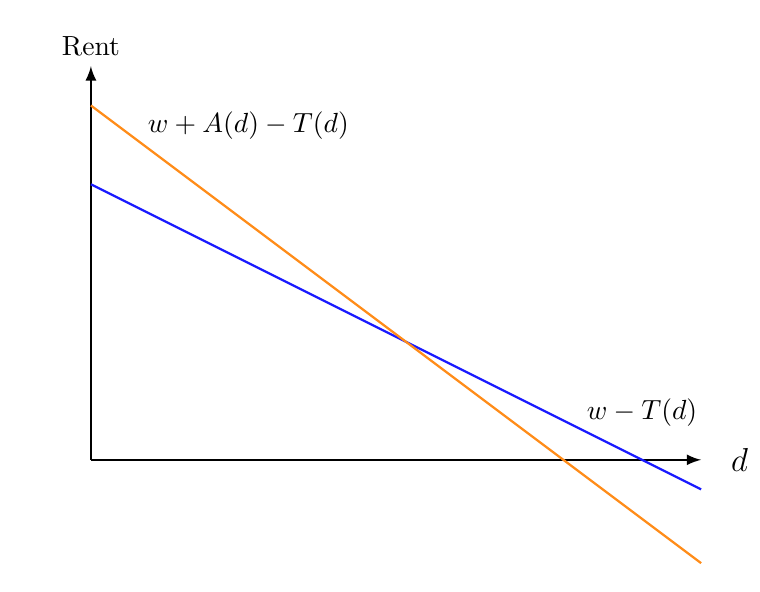
\begin{tikzpicture}[scale=.5]
\def\bndmax{5}        %https://tex.stackexchange.com/questions/68462/filling-a-complex-region-with-tikz
\def\bndmin{0.2}
\def \n {10}
\def \m {15.5}
\def \t {.5}
\def \th {1}
\def \w {7}
\tikzset{func/.style={thick,color=blue!90}}	
\draw [thick, latex-] (0,\n)node[above] {Rent}--(0,0);
\draw [thick, -latex] (0,0)--(\m,0)node[right=.25]{\large $d$};
%\foreach \xi in {0,..., \m} \draw (\xi,0)--(\xi,-.1)node[below=1]{\small$\xi$};
%\foreach \yi in {1,...,\n} \draw (0,\yi)--(-.1,\yi)node[left]{$\yi$};
%%\foreach \i in {1,4,9,16} {
	\draw[func,domain=0:\m] plot [samples=200] (\x,{\w-\t*\x});
%	\draw[func,domain=0:\m, dashed] plot [samples=200] (\x,{\w+\azero-\th*\x+\aprime*\x});

\node at (14,1.2){$w-T(d)$};
\def \azero{2}
\def \aprime {-.25}	
\tikzset{func/.style={thick,color=orange!90}}	
	\draw[func,domain=0:\m] plot [samples=200] (\x,{\w+\azero-\t*\x+\aprime*\x});
\node at (4,8.5){$w +A(d)-T(d)$};
%\node at(-.8,2) [left]{base $2^1=$};
%\node at(-.8,1) [left]{$2^0=$};
%\draw[dotted] (0,2)--(1,2)--(1,0); 
 \end{tikzpicture}
\end{center}
\caption{Rent profile with amenities}
\label{fig-amenity}
\end{figure}

 This model can produce variations on the standard result in the Alonso model. Figure~\ref{fig-amenity} illustrates a linear amenity function, $\mathbb{A}(d|N)= a-b*d$, that is convenient for illustrative purposes.  It shows how a particular amenity function might affect the rent profile, and hence city size and it allows simple experiments with the effect of increasing population on city size, wages and rents. 

In this case, amenity falls below zero in the outer regions of the city and, the geographical size of the city will be smaller. With a linear function, this happens if $\frac{a}{b} < \frac{w}{t}$. (a smaller city would have a secondary effect on wages, since with fewer workers' marginal productivity would be higher and therefore wages would rise. This would partially offset the initial decline in population.)
There would be a band of land around the city with negative amenity for commuters.\footnote{The very simple graphical result rests on several assumptions - no other housing expense, housing all the same size, wages all equal, preferences identical, transportation costs.}

The far more likely case is that $A(d) > 0$ when $w-T(d)$ falls to zero. In this case there is a band of residents around the city, outside of the population commuting to work. They do not travel to work,  do not collect a wage, but still enjoy the amenity of being close to a city. This might be a population of retired persons enjoying occasional visits and healthcare facilities.


\subsection{Neighbourhood amenity}
In Figure~{fig-amenity} the source of the amenity is at the centre of the city. We can easily imagine an amenity profile that is high for some neigbourhoods and lower for others, as in  In Figure~\ref{fig-amenity2}. The jagged area below the orange line is rent accruing to landowners. The variable rent comes not from a desire to be close to the source of the wage income but from household demand for local amenity.  
\begin{figure}[tb]
\begin{center}
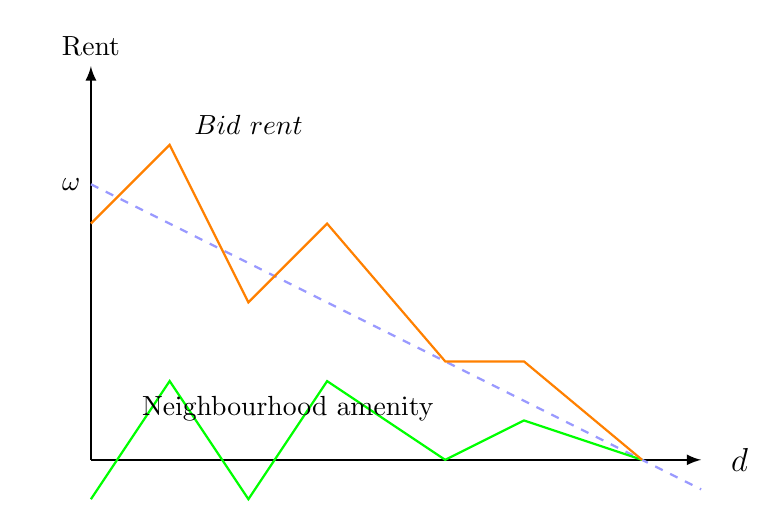
\begin{tikzpicture}[scale=.5]
\def\bndmax{5}        %https://tex.stackexchange.com/questions/68462/filling-a-complex-region-with-tikz
\def\bndmin{0.2}
\def \n {10}
\def \m {15.5}
\def \t {.5}
\def \th {1}
\def \w {7}
\tikzset{func/.style={thick,dashed, color=blue!40}}	
\draw [thick, latex-] (0,\n)node[above] {Rent}--(0,0);
\draw [thick, -latex] (0,0)--(\m,0)node[right=.25]{\large $d$};
% Basic Bid rent,
\node at(-.5,\w) {$\omega$};
\draw[func,domain=0:\m] plot [samples=200] (\x,{\w-\t*\x});
%NEIGBOURHOOD AMENITY
\draw [thick, green] (0,-1)--(2,2)--(4,-1)--(6,2)--(9,0)--(11,1)--(14,0);
\draw [thick, orange] (0,6)--(2,{7-2*.5+2})--(4,7-4*.5 -1)--(6,7-6*.5+2)--(9,7-9*.5)--(11,7-11*.5+1)--(14,7-14*.5);
\node [] at (5,1.3){Neighbourhood amenity};
\def \azero{2}
\def \aprime {-.25}	
% \tikzset{func/.style={thick,color=orange!90}}	
% 	\draw[func,domain=0:\m] plot [samples=200] (\x,{\w+\azero-\t*\x+\aprime*\x});
\node at (4,8.5){$Bid\ rent$};
%\node at(-.8,2) [left]{base $2^1=$};
%\node at(-.8,1) [left]{$2^0=$};
%\draw[dotted] (0,2)--(1,2)--(1,0); 
 \end{tikzpicture}
\end{center}
\caption{Rent profile with neighbourhood amenities}
\label{fig-amenity2}
\end{figure}
Financialization might or might not affect neighbourhood amenity. If it does it might have its effect by changing the ownership mix.

\subsection{Public provision of amenities}

Previous sections suggest amenities may work as a wage subsidy, potentially increasing output. Since employers will not willingly pay for urban amenities, some amenities may be financed publicly. It is common to introduce the cost of generating amenities as a tax on residents.  Since public amenities may be \glspl{public good} in the economic sense, the municipal government may be able to achieve significant wage economies with a small public expenditure.

A simple way to incorporate publicly provided amenities to make an amenity function that proportional to a fraction of public revenue, which is a fraction $\tau$ of the land value when municipalities depend on property taxes. Assuming a uniform property tax rate, total property tax revenue in a circular city are approximately $\tau(\phi+2/3 \omega)\pi \frac{\omega}{c}^2$. We can therefore include in the buyer's maximum bid function a fraction if this value. Property investors would not include this amenity component, but it would affect their decisions because amenity raises their net rent.

Notice that because amenity raises property values, in Ontario it does not raise tax revenue because the property tax rate is adjusted to balance the budget. This creates perverse incentives for municipalities \cite{blaisPerverseCitiesHidden2011}.


\subsection{An amenity sector}
Producing amenities takes resources. Some fraction of the workforce must be engaged in producing the amenity services. A simple approach would be to assume that the base employment that we consider demands a layer of amenities that represent the additional fraction of the population needed to provide the amenities - say 10\%  

Larger cities can support larger and more varied amenities, so that effect of amenities on property values might be larger in larger cities. At the same time, there are apparently economies of scale in the production of amenities \cite{kaufmannScalingUrbanAmenities2022}. We have no strong prior about how in amenity sector would be affected by finacialization of housing.  An effect might work through changing ownership.


\section{Research on amenities}
% There is a great deal of research on amenities. In this subsection mention a few that seemed noteworthy. 
Most of the literature on amenities deals with livability and the benefits for the individual. There is a strand in the literature, however, that links amenities to growth. In 1954, for example, Edward Ullman \cite{ullmanAmenitiesFactorRegional1954} published  ``Amenities as a Factor in Regional Growth,'' an article that came to be seen in the geographical literature over the following 50 years as prescient \cite{walcottCommentsEdwardUllman2010} for introducing the notion that amenities could be an important mobility magnet. 

Many have since extended this approach. Richard Florida, in a series of articles and books beginning in 2002 \cite{floridaCreativeClassEconomic2014, floridaEconomicGeographyTalent2002, floridaCompetingAgeTalent2005} examined the notion that urban growth depended on attracting the creative class and that in turn rested in part on the amenities a city offered. A 2008  Statistics Canada study, `Cities and Growth: The Left Brain of North American Cities,' Beckstead et al \ found substantial differences in average growth for cities with higher cultural employment and urban amenities.  Clark et al \cite{clarkAmenitiesDriveUrban2002} argue that much of Chicago's recent growth to 2003  should be attributed to reforms instituted by Mayor Richard M.  Daley explicitly linked to amenities and quality of life issues, including parks and schools. Abouy \cite{albouyWhatAreCities2016} finds that wage and housing cost differences across metropolitan areas are accounted for more by productivity than quality-of-life differences, however. 

Beckstead et al  \cite{becksteadCitiesGrowthLeft2008} identify amenities with the unexplained variastion in median urban house price after controlling for median household income.\footnote{  The basic premise would be that after conditioning on household income, variation in home prices across cities would be a function of the relative attractiveness of these places. The residuals yield a continuous ranking of cities based on the estimated variation in urban amenities.} Rappaport \cite{rappaportConsumptionAmenitiesCity2008} presents empirical evidence that amenities do support high-density levels, and that amenities cause approximately one-fifth of the cross-sectional variation in metro population density. 


% Molotch's (1976) metaphor suggests that the city is a machine geared to creating growth, with growth loosely defined as the intensification of land use and thus higher rent collections associated professional fees and locally based profits. Many urban economists, planners, and political scientists have made similar arguments (e.g., Bradbury, Downs, & Small, 1982; Mollenkopf, 1983; Stone, 1989). However, a quarter century later in the contemporary competition among US cities, the growth machine model has lost much of its power.
  


\newpage


% \chapter{Notation}
% \section{Notation for Urban and Production Sectors}
\newpage
\begin{longtable}{lp{10cm}}
\caption{Notation}                       \\
\hline           &  \textbf{Productivity} \\ \hline
$K$              &  Capital               \\ 
% $L$            &  Labour                \\
$N$              &  Population, equals labour \\ %, $L$          
%$\Lambda$    &  Labour-augmenting agglomeration effect \\
$Y=A K^{\alpha }N^{\beta }$  &  a Cobb-Douglas Production function \\ %Urban output            \\
$\alpha$         &  Elasticity of output with respect to capital          \\
$\beta$          &  Elasticity of output with respect to labour           \\ % vs effective labour
$\gamma$         &  Elasticity of agglomeration with respect to labour    \\ % , $\Lambda(n)$, for illustration \\

% $L$              &  Labour supply \\ %the number of workers, which, in the standard circular city model, equals the number of lots of size $s$  when workers live on identical individual lots. % Unless $d^{max}>d^*$ v  \frac{\pi}{s}(\frac{w}{{c}})^2 =
$n$  &  Number of workers at a firm \\
% $n_i$  &  Number of workers employed by firm $i$ \\
%$n=\sum_i n_i$  &  Number of workers, the urban population in the model \\
% $\#f=\frac{n}{n_i}$&number of identical firms \\ %not used
% $f$  &  Number of firms =1 \\
% $n =f n_i$  &  Aggregate labour \\
% $n^\gamma$ & The labour-augmenting agglomeration effect,  modelled as an exponential function of the number of people \\
% $\Lambda(n)n_i$ &  Effective labour for firm $i$ \\
% $\Lambda'=\die{\Lambda(n)}{n} $ & Derivative of the labour-augmenting agglomeration effect\\

%%$Y_i=K_i^{\alpha }(\Lambda(n)n_i)^{\beta }$  &  Urban firm $i$'s output \\

%%$Y=\frac{n}{n_i}K_i^{\alpha }(\Lambda(\sum_i n_i)n_i)^{\beta }$  &  Aggregate output of all firms in the city \\
% $\die{Y}{n}=\beta\frac{1}{n} Y  \left( 1+ \frac{n\Lambda'}{\Lambda} \right)$  &  Social marginal product of labour \\
% $Y_i=K_i^{\alpha }(\Lambda(n)n_i)^{\beta }$    &  Urban firm $i$'s output \\
% $\die{Y_i}{K_i}	=\alpha \frac{1}{K_i} Y_i $  & Marginal product of capital for firm $i$ \\
% $\die{Y_i}{n_i}	=  \beta\frac{1}{n_i} Y_i $  &  Marginal product of labour for firm $i$ \\
%%$\eta=\frac{n_i\Lambda'}{\Lambda}$  &   Marginal agglomeration effect on a firm's output of increasing it's own labour stock \\
% \hline
	% &\textbf{Amenity}\\ \hline
% $A(d, n)$   &  Agglomeration amenity          \\

\hline  0 &  \textbf{Labour market}                \\ \hline %and urban stucture??
$\psi$            &  Rural subsistence wage                             \\  
$\omega$          &  Urban wage premium          \\
${c}$             &  Transportation cost per unit distance \\ % Was $\tau$, and $trans$. Considered $\gamma, \xi, \zeta$.
$d$               &  Distance from city centre   \\
$d^* = w/{c}$     &  City extent \\ %, the maximum distance commuters will travel \\ % Maximum distance commuters will travel \\ % to get the wage premium \\
% $\mathcal{R} = \omega - {dc}$ &  Rent at distance ${d}$ \\ 
% $\zeta$          &  Population density at distance $d$     \\
% $s$              &  Lot size      \\
% $\psi$  &  ?Per-period cost of a unit of productive capital \\
% $\omega + \psi$  &  Urban wage including rural wage \\ %***
% $\textit{t}$ & {\color{red}transportation cost per km} \\%use   c?
% $w^n=\omega-{dc}$ & Wage  premium net of transportation costs \\
%% $\Omega=\frac{\omega+\psi}{\psi}$  &  Ratio of the urban wage to the  cost of capital \\
%% $\Pi$	   &  Profit \\
%% $ER$	   &  Excess return to capital \\ 
% \hline &\textbf{Spatial structure in the circular city} \\ \hline		
%% $d^{max} = \omega /{c}$  &  Maximum distance commuters at which residents enjoy the urban amenity \\
%% $d^{**} = max(d^*, d^{max})$  &  radius of the city \\
%% $U$                     &  Worker utility **\\ %, a function of location and prices \\
%% $U^{urban}=U^{rural} $  &  Migration equilibrium assumption ** \\
% \hline & \textbf{Labour market} \\ 

\hline           & \textbf{Financial market}             \\ \hline
$P_W$            &  Warranted price for a property       \\
$P_B$            &  Bid price                            \\ % was P^{bid}
$P_A$            &  Asking price                         \\
$P_M$            &  Realized market price                \\
$P_M^e$          &  Expected market price                \\
% $P$            &  Price of a property                  \\ 
% $\dot P$       &  Rate of price growth              \\ % was $\dot p$  
% $\mathcal{C}$    &  Capital gains                     \\ % was C
% $\mathcal{C}_N$  &  Net capital gain, $C -$ net rent  \\
% $M$              &  Mortgage                          \\ 
% $m$              &  Mortgage share, the share of the property price that can be borrowed, which is a function of wealth  \\ 
$\mathcal{R}$    &  Rent                              \\
$\mathcal{R}_N$  &  Net rent                          \\
${R}^w_N$        &  Warranted rent                    \\
$\rho$           &  Rent ratio                        \\
$\phi$           &  \Gls{rent share}                  \\
$\mathcal{O}$    &  Operational costs                 \\
% $\theta$         &  Operations ratio                  \\ % was $\kappa$ became b
$\mathcal{T}$    &  Taxes                             \\ % was $\Sigma, \Xi$  
$\tau$           &  Property tax share                \\ % was t then $\sigma, \xi$  b
% $\tau$            &  Annual tax rate on rent and home \\ % Was $c$ 
$r$              &  Interest rate                     \\
$\delta$         &  Individual's subjective \gls{discount factor} \\
% $W$            &  Wealth                            \\
% $\psi$         &  Fraction with rent/operating costs\\
$t$              &  Time                              \\

W & Wealth \\
m & Mortgage share \\
M & Mortgage \\
S & Savings \\
% \mathbb{C} carrying 0.28, max_mortgage share, wealth_sensitivity

$\mathbb{T}$     &  Time period                       \\

$a$       &  Share of subsistence wage  used for land and building \\
$b$       &  Maintenance share of share of subsistence wage \\ % A cost. Includes water, electricity, heat? 
% $wage_share$     & OLD Share of the agglomeration effect that goes to workers. \\

\hline
\color{black}
\end{longtable}  

\newpage

\begin{longtable}{lp{10cm}}
\caption{Rent}                                                            \\
\hline
$\omega-{dc}$                &  Warranted (economic) rent                \\
$\mathcal{R}=\omega-{dc}$    &  Equilibrium rent payment of tenant       \\
PDV                           &  Present discounted value                 \\  
$\mathcal{R}^T$               &  PDV of rent collected over period $T$    \\ 
$\mathcal{R}^T_N=(1-\kappa-\sigma)\mathcal{R}^T$  &  PDV of net rent collected over period $T$ \\
\hline
\end{longtable}

\begin{longtable}{lp{10cm}}
\caption{Bidding mechanism notation}                                          \\
\hline
$\mathcal{R}_N$  &  Net rent                                                  \\ % was NR
% $P_0$            &  Purchase price for a property                             \\
% $P^T_e$          &  Expected price at the end of period $T$                   \\
$r^{prime}$         &  Prime interest rate                                       \\
$r^{target}$     &  Investor or banks target interest rate, $\bar r + margin$ \\

$r_i$            &  Agent $i$'s personal borrowing rate                       \\
$r_i^T$          &  Agent $i$ interest rate compounded over a period $T$      \\
$r_i^{disc}$     &  Agent $i$'s subjective discount rate (which may equal $r_i$) \\
$r_\delta$       &  Discount rate                                             \\ % was $discr_i$
$\delta_i^T$     &  Discount factor for agent $i$ over period $T$             \\
$m^W$            &  Wealth-based share of home price a worker can mortgage    \\ % $= m_i(W_i)$
$m^\omega$       &  Income-based share of home price a worker can mortgage    \\ % IS_i   IS_i(\omega+\psi)$$
$m_i = min(m^W_i, m^\omega_i)$  & Mortgage, the share of home price worker $i$ can mortgage \\

\hline
\color{black}
\end{longtable}  
Notation: 
Agent counts and indices are subscripts.
Values related to time are superscripts, time as a continuous 
variable is small, a period is capitalized e.g. the period $T$ of some number of years. 
In general values are capitals, rates are small letters.

% It might be better to use the subscript $m$ for `market'.  for warranted rents



 

% % Short
% % \chapter[Future Work]{Future Work}
\label{appendix-future-work}



In  this chapter, we discuss potential extensions of our basic model.  Models are by nature combinatoric: every added element involves making a choice among alternative assumptions and implementations. A model incorporating in binary choices is one of an implicit family of $2^n$ alternative models. We have sharply restricted our model  in order to focus on one process of significance, financialization.  This is in part so that we can explain and justify each assumption that we use, and in part because only sharply restricted models produce understandable results. 
% Those results are condition on the specific set of assumptions to ensure that 
We have designed the model to  accommodate a range of extensions that are either theoretically or interesting or important for policy-makers. 



Figure~\ref{fig-logic-extensions} illustrates  five general types of extension. The first is to move from a static population to a model with population pressure. This appears on the left as a group of three new subroutines with connections to the elements of the model most directly affected. Some links are left out to keep the figure readable. Examples of omitted links  are the channels through which  population affects labour supply and savings.  


A second class of extension would introduce a housing production sector. This appears on the right side of of the figure linked to the banking sector. It requires adding a dynamic housing  stock. 

A third major class of extensions, separable from production is to introduce variation of housing form,  density and amenity. Zoning restrictions and building codes are related. Many questions about who gets what housing arise at this point. 

{\newpage\thispagestyle{empty}
\vspace{-1.5cm}
\begin{figure}
\vspace{-4.5cm}
\begin{adjustwidth}{-0.24\textwidth}{-0.2\textwidth}
\centering
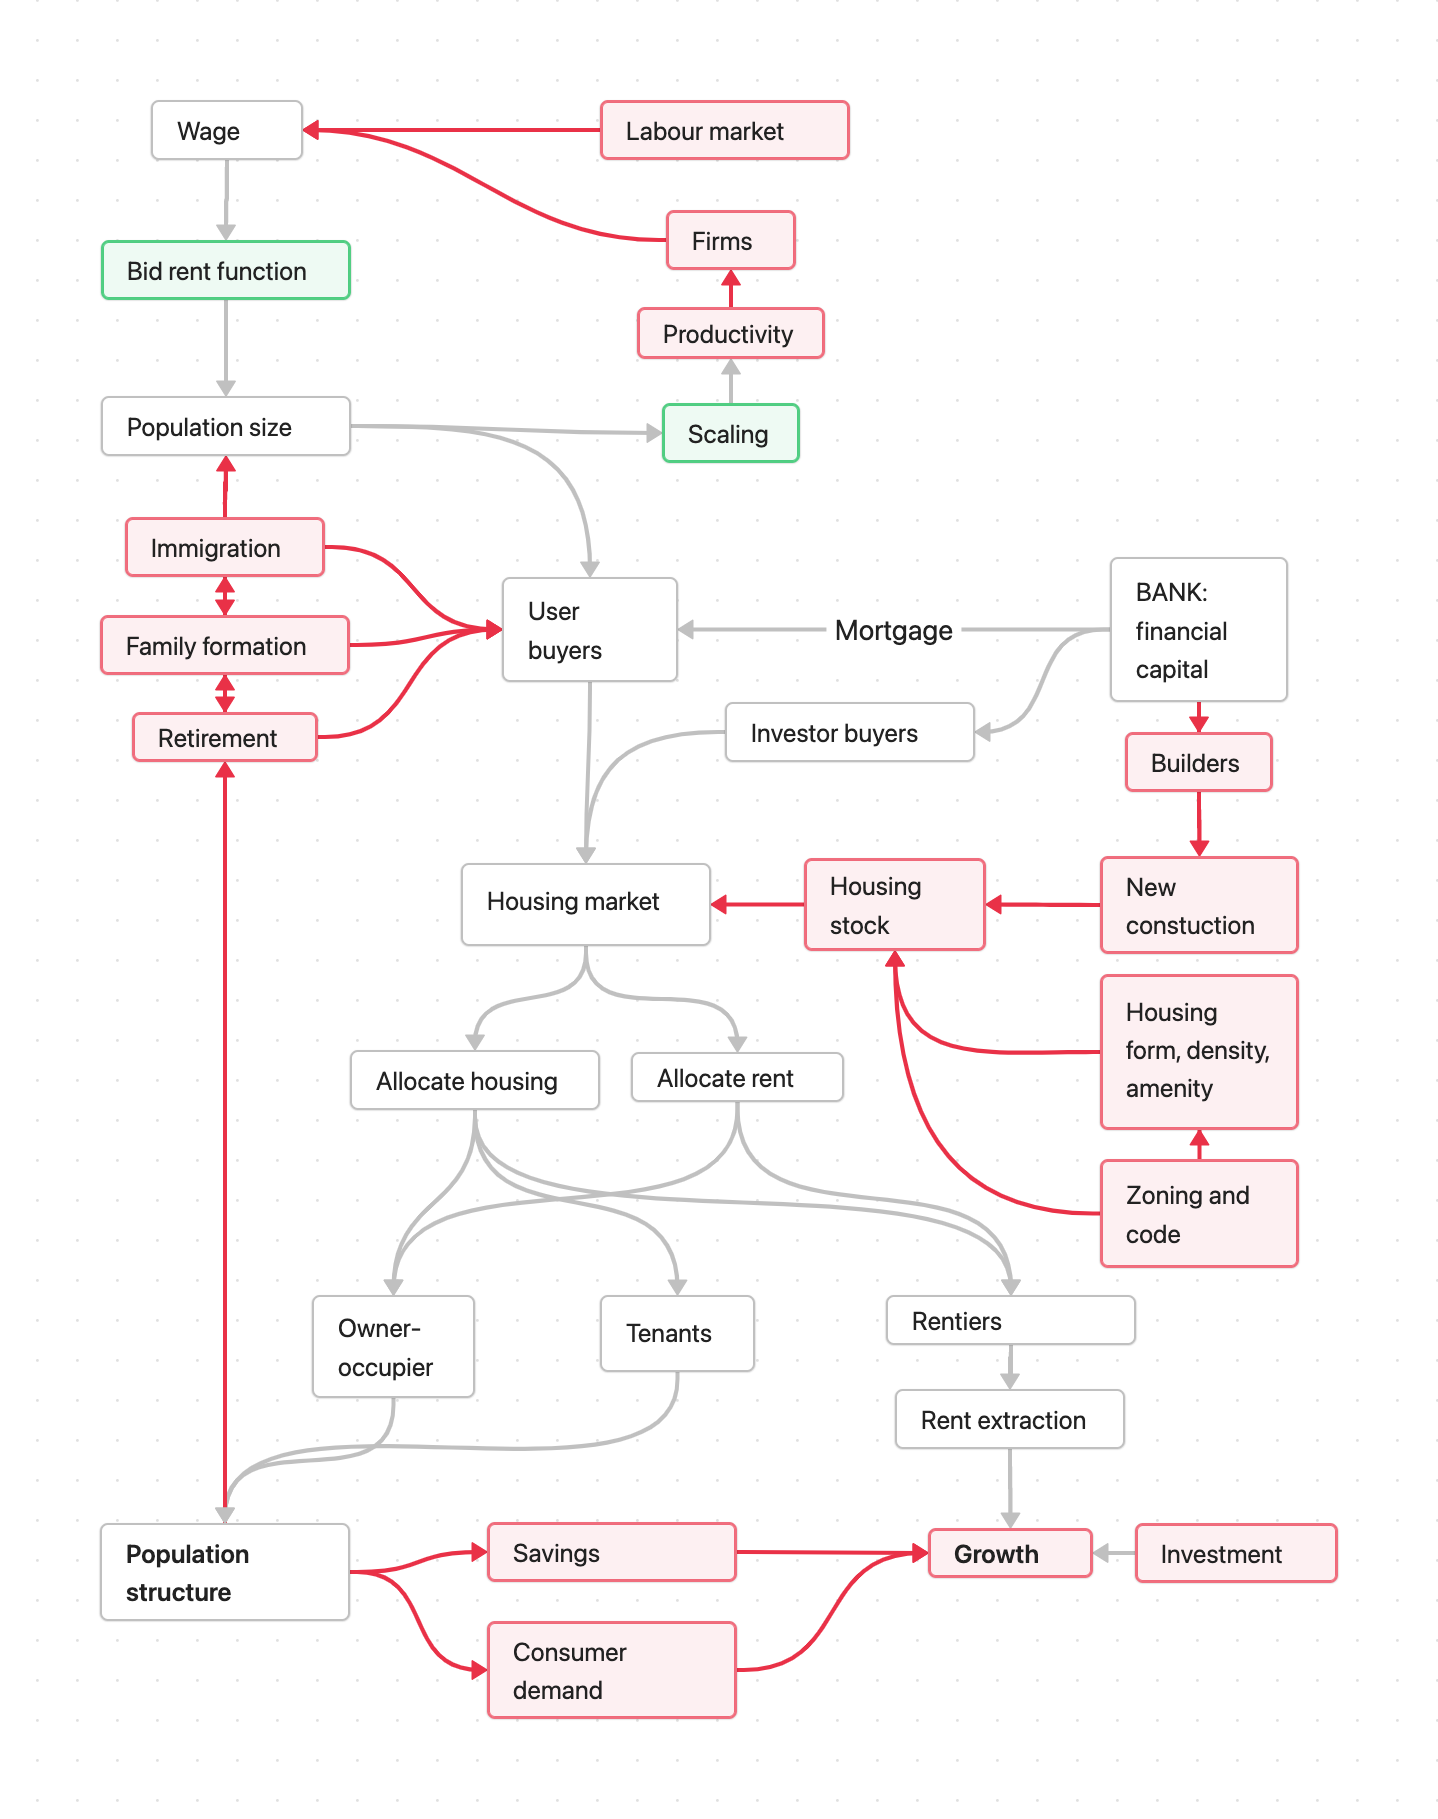
\includegraphics[scale=.22]{fig/extensions.png}
\end{adjustwidth}
\caption{Extensions}
\label{fig-logic-extensions}
%\pagestyle{headings}
% \usetikzlibrary{positioning}
%\begin{tikzpicture}[remember picture,overlay,shift={(current page.north east)}] \node[anchor=north east,xshift=-1cm,yshift=-1cm]{\includegraphics[width=1cm]{example-image-a}};\end{tikzpicture}

\end{figure}
}


At the bottom of the figure we introduce consumer demand linked to the population structure and feeding back to growth. Savings behaviour becomes more  complex when consumer demand is made endogenous and with as more complex population structure.

The fifth block of extensions illustrated in Figure~\ref{fig-logic-extensions} would replace the simple, scaling-based transmission mechanism in the Alonzo-Jacobs cycle with explicit firm and labour market behaviour. This class of extensions is obviously linked to population structure. It leads to consideration of firms that produce different products, some for export some for the local market, and to multiple types of labour.

Linked to the labour market and production system is the possibility of introducing competing cities. 

It should be clear that each of the extensions we suggest is potentially as complex as our core model, and each brings with it a collection of additional assumptions. We would argue that none of them would change our qualitative results greatly, although each would deepen our understanding of mechanisms and of the detailed impacts.


\section{Population pressure } 
Our basic model does not have a growing population. This conveniently allows us to isolate certain effects of financialization. Population pressure is one of the drivers of financialization because it amplifies speculative gains, however. As a result, one of the first extensions must be  to introduce population pressure.

There are two sources to consider: 
\begin{enumerate}
\item agglomeration effects that increase the wage and attract workers faster than the housing stock can respond. 

Worker agents from outside the city can always consider moving and accepting a job. 
% QUESTION - how to manage the flow of new agents?
%, or can make more from rents and moving away
\item immigration pressure
\end{enumerate}
under the  first, agglomeration economies drive population while under the second, population growth may drive agglomeration.

The growth of the housing stock will generally lag population growth, generating price effects and stock dynamics.

Agents will respond to increases in demand conditions. The perception that the market is tight or that prices are rising may lead to higher bids and reservation prices and shift results in favour of sellers.  


%Buyers could consider neighbourhood pressures, demographic changes, changes in job location, desire for amenity etc. in their assessment of housing need. 

%With multiple bids agents can place the most competitive bids on those homes they prefer. If they have higher urgency they place strong bids on more homes. 

%Next buyers request a selection of homes to consider from a real estate agent. Those with higher need for housing look at more homes. The real estate agent offers a selection of homes based on the agent's requirements. A randomness parameter determines how many divergent houses are also considered. When the parameter is 1, the selection of homes is fully randomized, When it is 0, the agent sorts all available homes and offers those which fit the agents budget, space, and other requirements best.


\subsection{Retirement investors and private investment properties}
The simple population turnover in our model can be replaced with a more complex set of possibilities at the agent level.  At retirement,  agents can be allowed to may choose between selling their home, renting it as an income property, or if there is sufficient amenity value for them, staying in the city. Implementing these choices complicates the agent decision and the resulting housing distribution but require few changes to the rest of the model.

\section{Housing production}

\section{Differences in density, housing form, and neighbourhood amenity}
Much of what is interesting in a city is the rich variety of housing forms and neighbourhoods and the varied populations that occupy them. Our model has a single form of housing and an undifferentiated populations, allowing us to differentiate the housing system in specific ways and study the interactions between the built world and the population. We are convinced that few of the possible extensions could affect our qualitative results. 

Nonetheless, in our agent based model, in which every lot is  addressable, it is simple to introduce zoning boundaries, local amenities, different densities or housing qualities and homes of different sizes. Hundreds of experiments are possible exploiting  the extensibility we have carefully conserved.  

We can ask what would be the effect of a hard zoning boundary and what would be the effect of suddenly relaxing it. We could explore the effect of speeding the rate of conversions from one size  home to another, or of locating high density pocket on a transportation route. Many significant urban policy questions could be examined with a limited amount of additional programming. 

\section{The consumer city}
Much of the demand for what is produced in the city is local consumer demand.  Our model has assumed there is production only for a perfectly elastic export demand. Consumer needs are buried in the subsistence wage. 

A minimal extension would be to introduce a second sector representing local consumption demand. A share of locally generated income would support production for the city's population. The labour force would be split between the two sectors and both productivity and wages might differ across sectors. 

A more complex treatment would introduce a range of service, entertainment and retail producers. This might be done monopolistically competitive firms \'a la Dixit and Stiglitz \cite{AvinashK.Dixit1977MCaO}.



\subsection{Distribution of rents}
Rents go to landowners, with a share taken for maintenance and taxes.
Rents may also be taxed, could be shared between multiple owners, etc.
 %\note{REPHRASE? rent is  extracted from the coalition of capital and workers.} % Rents may also be taxed, could be shared between multiple owners, etc. 
%The rents are captured by landowners.  The capture of rents by landowners is common buy not necessary. 
In principle the gains from urban productivity and amenity can be allocated as social wealth through shared ownership, as is often done on a small scale with cooperatives and land trusts, distributed to all citizens through something like a social wealth fund, or captured in taxes or fees as Henry George suggested. 
%The rents would otherwise go to labour and capital.





\subsection{Urban Savings - Contributions?}
THIS IS A CONTRIBUTION, BUT ALSO A DISCUSSION OF ONE WAY THIS WORK COULD BE EXTENDED, MIXED WITH A BIT OF MODEL DESCRIPTION

Conventional growth models specify a savings/investment mechanism at the national level. To our knowledge, this has not been done for the city level. We require  savings at two levels. First, since we want to incorporate  households home ownership and a relationship to the financial sector through mortgages, We specify a savings rate out of the spending we have isolated in the `subsistence wage' This means that both urban and rural workers accumulate savings, that savings are age-dependent, making the size of mortgage available also age dependent. 

Homeowners in addition have equity $E=P-M$ in their homes.  ({\color{red}Should newcomers also have equity? or is it built into the savings. Clarify this.} 

A second level of saving is the  investment in capital out of the city surplus. Even raising this question puts us into terra incognita. There are many  channels through which surplus flows into productive investment in the urban contest. One is through public investment in infrastructure. We have discussed how falling transportation costs increase surplus generation. Investments like this are made slowly and take effect over time periods much longer than our model is concerned with.  We can set a property tax rate   that we will assume is sufficient to maintain the stock of infrastructure.

Public and private investment in human capital is largely urban as well, but as with infrastructure, investment and response take effect over time periods much longer than our model is concerned with. 

Private sector innovation in technology, marketing, or products draws on local saving less but still significantly on local savings. We have little in the way of theory or empirical research on this channel. Lags between investment and any rise in the urban wage premium are almost certainly long and variable. 

We deal with this issue by linking local capital ownership with the scale factor. It is known that local ownership is associated with local investment. We will assume that local capital ownership, which consists in part of local ownership of the housing stock, can be proxied by homeowner equity as a share of local. 

\subsubsection{savings and retirement behaviour}
Agents fund their retirement from savings, as well as returns on their home if they have one to sell. Savings may be invested in a pension fund, or in local property,  depending on expected risks and returns. In the real world, financial institution manages most pensions, investing in the market or in property.  All this institutional structure is probably most easily handled by implementing a savings account for each agent. We are not interested in the detailed investment behavour for the financial sector.% either in the stock market, or in pensions.

%Institutional and individual investors can access debt. %

We could also consider a case where outside money can come under institutional management, not just local retirement savings. A parameter would control the inflow of additional money beyond local investment in the pension fund. 



\section{Making  labour market and firm behaviour explicit }
We have carefully developed the link between neoclassical growth theory and the literature on urban scaling \cite{bettencourtIntroductionUrbanScience2021} and  We then imposed the scaling result on our model.  We force the model to conform to the empirical data on the relationship between population and productivity. This amounts to black-boxing the entire production and labour demand sector as well as the construction and housing production sector. 

This made sense because our focus  was on the housing market and the financial sector, but the model we have constructed will allow us to ``fill the black box'' with more complete models of the production and labour market to see how they compare to the empirical data. 

The  scaling  literature also provides relationships between density and population and infrastructure cost and population that we can explore in the same way.

In the scaling literature, these relationships are increasingly theorized in terms of network effects, which is perfectly consistent with the Jacobs analysis and the more recent neoclassical growth modeling.


\subsection{The transmission puzzle}

The transmission of productivity increases arising from agglomeration effects  to the urban wage through firms, can be modelled in many ways. The agglomeration effects are external to the firm and therefore likely to be unexpected. If  firms underestimate the marginal product of labour, labour productivity will be greater than expected, output will be higher than planned output, and revenue and profits will therefore be higher than expected. Excess demand will attract more productive capital which in turn will demand more labour,  Rising labour demand drives up the wage. The agglomeration effect driving growth is essentially a public good in which individual firms will under-invest. This raises a policy challenge that we leave for others. CLARIFY - ALSO STILL A FOOTNOTE IN MODEL SECTION. CUT OR REF THEiR IF MOVING HERE.

 It is straightforward to compute the rate of excess return for  this model. 


\begin{figure}
    \centering
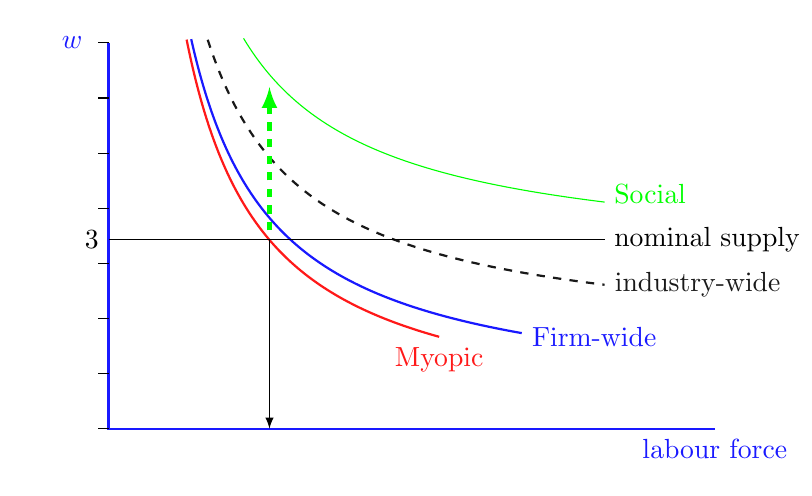
\begin{tikzpicture}[scale=.7]
%\def\bndmax{5}        %https://tex.stackexchange.com/questions/68462/filling-a-complex-region-with-tikz
%\def\bndmin{0.2}
\def \Y {7}  % height of y axis pecent
\def \W {15}  % length  of x axis
\def \Wbar {3} % jmeam wealth
\def \omega {3}
\def \A {1}  %was .5
\def \B {.5}

\draw [thick, color=blue!90] (0,\Y)node[left=.2cm]{$w$} -- (0,0)--(\W-4,0)node[below]{labour force};  
 \foreach \yi in {0,...,\Y} \draw (0,\yi)--(-.2,\yi)node[left]{};
 
\tikzset{func/.style={thick,  color=blue!90}}
% \draw[ func, domain=.2:\W-6] plot [samples=200] (\x, 2*\x^.5)node[below=.1, right]{SUPPLY};

\tikzset{func/.style={  color=green}}	
\draw[func, domain=2.45:\W-6] plot [samples=200] (\x, 10/\x+3)node[above=.1, right]{Social};

\tikzset{func/.style={thick, dashed, color=black!90}}	
\draw[func,domain=1.8:\W-6] plot [samples=200] (\x, 10/\x+1.5)node[ right]{industry-wide };

\tikzset{func/.style={thick, color=blue!90}}	
\draw[func,domain=1.5:\W-7.5] plot [samples=200] (\x, 10/\x+.4)node[below=.05, right]{Firm-wide};

\tikzset{func/.style={thick,color=red!90}}	
\draw[func,domain=8.5/6:\W-9] plot [samples=200] (\x, 10/\x)node[below]{Myopic};

\draw[](0,3.425)node[left]{$\omega$}--(9,3.425)node[right]{nominal supply };
\draw[thin,latex-](2.92,0)--(2.92,3.425); %a vertical labour supply
\draw[ultra thick,dashed, green,-latex](2.92,3.6)--(2.92,6.2);
%\draw [blue,  thick](13, 8.3)--(15,8.3)node [right, black] {\small A=\ 1,\ B=0.5};
%\draw [green, thick](13, 7.6)--(15,7.6)node [right, black] {\small A=.8, B=0.8};

%\node at (5,-1.5){Resulting in  profits, expansion, and/or entry: the city grows};
 \end{tikzpicture}
\caption{Multiple marginal products.}
\label{fig-marginal-products}
\end{figure}



Figure~\ref{fig-marginal-products} illustrates the problem. We can  make a distinction between the myopic marginal productivity curve observed by at the shop floor level and  the firm-wide effect of adding a worker. The red curve labeled ``Myopic'' represents the declining direct marginal productivity of labour as in might be observed by a shop manager, who could report how much more output one with one worker one lathe would produce. The blue line above it labeled ``Firm-wide'' represents the actual effect on firm productivity that arises because the new worker makes other workers in the firm more productive. This addition to output would be observable for managers reviewing the firm's performance over time. ' 

We can go on to consider the slower and distributed effect on closely related firms, which would raise any estimate of marginal product.  If there are 10 other firms and a new worker  has a small spillover effect  $\epsilon$ on each,  the spillovers raise the industry  marginal product  by $10\epsilon$. Each of the  10 other firms  enjoys  an additional $10\epsilon$ gain in the marginal product of their workers. This should lead to additional hiring by other firms.

Finally, expanding our view another step, we notice that if each of the  10 other firms hires one worker who produces an additional  $10\epsilon$ gain in output for all firms, the total spillover effect would rise by $100\epsilon$. The social marginal product of a single hire is indicated by the green line. 



\section{The system of cities}
Modern cities are not lonely and autarkic  beasts wandering their own exclusive territory and unconnected to others of the species. They are one is a global system of cities that compete and complement each other. Information, capital and even labour flows between cities are large. Henderson Abdel-Rahman\cite{Henderson1972Sizes}, Abdel-Rahman \cite{abdel-rahmanAgglomerationEconomiesTypes1990}, Fujita \cite{fujitaMonopolisticCompetitionModel1988}, Fujita, Krugman, and Venables \cite{fujitaSpatialEconomyCities1999}, and Fujita and Thiess \cite{fujitaEconomicsAgglomeration1996} among others provide models for expandingh the model in this direction.



\subsection{Taxes, municipal government, public goods, and productivity,}
This is a major issue with considerable development in the economics literature. Property taxes reduce the net locational value that flows to an individual owner but provides services and wages that make the city attractive. 

(create a regime where particular groups have an advantage)

Localized tax advantages can move a share of financialised investment into private consolidation of land.
including the structure of taxes for investment properties, institutional investors, individuals, etc.




\section{TO  METHODOLOGY?: Distribution}% not the right word
ABMs can be run multiple times to produce distributions of expected outcomes, which makes them valuable in planning exercises. They also do not require that we use a representative agent to make them tractable. Our model is intended to be elaborated  for such use. 

extensions
what it is
why it would be great to model
why it doesn't matter for our core results

\section{A possible typology of models and experiments}
While there  are many variations on the basic urban model and many potential experiments with each model there are only a few of immediate interest if the goal is to text the ``resilience'' of equilibria.

These models may exhibit irreversibilities in variables such as distribution, homelessness, city form, and class structure. 

The basic strategy for examining the system resilience is to shock a model (experiment) and then see if diagnostic variables recover. (This needs more precise expression.)

The first task is to select a subset of models an experiments that are of particular interests with respect to.

The second is to construct a model that allows those case to be examined. Ideally the model would be easily adapted to other experiments.

The following is a an attempt to develop a typology with a clear progressive structure.

Feedback - wealth allows upgrading. This advantages the rich. Maybe this 

\subsection{Models}
\begin{enumerate}
\item \textbf{A: The basic model}

The workhorse of urban economics is the circular city model. Some feature of the central place generates rents. It may be that it is the only employment centre. It may be economies of scale to a single activity or synergies arising from various externalities\footnote{We are interested in agglomeration economies. The wage  structure would then be related to the population or industry  structure. Externalities driving agglomeration may be classified  into two types, the  or so-called ``Marshalian''  and ``Jacobs'' externalities.}. 

In the simplest model, the central place pays a uniform wage, $w$ to all employees, who have identical preferences and transportation costs. $w$ is an attribute of individual residents. Residents  purchase or rent equal quantities of land at differing locations $l$ for identical housing.  

There are transportation costs $T$ that depend on distance from the  central place, so land close to the central place is more attractive than land farther from the central place.  

The equilibrium concept is that a market with identical individuals with identical incomes and transportation costs will result in identical utilities. The result is that land rent must decline with distance from the central place to offset rising transportation cost. 

The size of the city is determined by population and lot size. Income and transportation costs will interact with lot size. The basic model can be initialized by matching the number of properties to the size of the population. 

If population exceeds the number of properties there are three margins to consider
	\begin{enumerate}
		\item The land supply can increase. There may be a conversion cost
		\item The land per-capita may decrease. This is not simple in a city with land-use regulations, zoning, and fixed capital in homes. A conversion process has to be defined
		\item A homeless population can emerge. 
	\end{enumerate}

It is convenient in this model to use a \gls{Cobb-Douglas} utility function that has the property that a fixed fraction of income is spent on housing.  We can start with the assumption that earnings are fixed for the lifetime at the one-period wage, $w$. Then total spending on housing is $\beta Y, \beta <1$ and $ Y=w$. Let the transportation cost for a specific location $l$ be $T(l)$. The  equilibrium price at that location will be $P(l)= \beta Y-T(l)$.

It is convenient but not necessary to assume that land outside of the residential limit is costless. It is common to assume a fixed price for agricultural land. 

There is no fixed boundary and the size of the city is determined by the utility that can be achieved in competing regions of competing

\item \textbf{Y: The basic model with Income Differences}
This will result in segregation by neighbourhood depending on income. 

Income can be purely earning, which requires a distribution of $w$ across agents. Income  might include investment income, which  a private rate of return and a distribution of assets across agents. \footnote{A more subtle model could allow individual wages to be linked to the agglomeration of other workers - say engineers. we can imagine a city that has centres of agglomeration by profession or by complementarity. Depending on the production function, this should emerge endogenously.}
\footnote{Sufficient investment income could lead individuals to locate in cheap properties at the edge of the city.  Income might also be invested in property affecting the quality of a unit. This would require incorporating unit quality in the attribute list for each property, and introducing a quality preference  in the attribute s of residents.}

\item \textbf{L: The basic model with Locational Preferences}
This will result in segregation by neighbourhood depending on preferences.

One version would be include distance to the edge of the city as an amenity in the utility function. Another would be to locate amenities within the city. These would lead to higher prices near amenities.

A natural variant would be to have earning depend on location. If there were several locations  a polycentric city would emerge.

\item \textbf{T: The basic model with varied transportation cost }
This will result in segregation by neighbourhood depending on income and Transportation costs. Experiments include cars for the rich and  transit. 

Diagnostics include change in total transportation cost and differential welfare effects.

\item \textbf{R: The basic model with a rent-own choice}
This may result in the emergence of classes. Agents must have the capacity to borrow to purchase. Attributes of the agents and must now include  net assets,  an available interest rate, and a permissible mortgage.

We imagine a banker setting the mortgage rates and size. This can be done at the beginning of each period for each agent. 

With no income differential we expect equal utiliites

\item \textbf{YR: The basic model with earnings (Y) differences and a rent-own choice}
This model is likely to generate diverging classes as income differentials permit some to capture land rents from others. This is highly likely if borrowing costs decline with income and asset ownership.

\item \textbf{L: The basic model with variable lot size}
This is achieved by making lot size a choice variable for households, in which case we will get a trade off between transportation cost and lot size and distance. Results for this model are known. Density  falls with distance from the centre. 

\item \textbf{YL: The basic model with earnings (Y) differences and variable lot size}
The wealthy choose larger homes and lots farther form the centre

\item \textbf{S: The basic model with constant lot size and variable density}
This is achieved by allowing stacking of housing units. Results for this model are not known. This introduces a step change in housing form, and emphasizes unit size.

This model should produce some interesting spatial patterns, especially if couples with the possibility of secondary central places.

\item \textbf{YS: The basic model with earnings (Y) differences, constant lot size and variable density}

This model should produce some interesting spatial patterns, especially if couples with the possibility of secondary central places.

\item \textbf{IR: The basic model with outside investors and rent-own}

\item \textbf{IYR: The basic model with outside investors, earnings differentials and rent-own choice} This model is of interest if borrowing costs decline with income and asset ownership.
\end{enumerate}
\subsection{Experiments}
There are various experiments of interest. You will have to pick key ones. It is not necessary to do all of them in every model. 

	\begin{enumerate}
		\item increase population
		\item increase wage
		\item add hard boundary (limit land)
		\item Introduce differential incomes
		\item Introduce differential access to capital
	\end{enumerate}

% \newcommand{\cred}{\cellcolor{red!30}}
% \begin{table}[htp]
% \caption{Potential experiments: \textbf{Pick some}}
% \begin{center}
% \begin{tabular}{|c|c|c|c|c|c|}\hline

%   &\multicolumn{5}{c|} {experiments}\\ \cline{2-6}
% Model  &1 &2  & 4 &4  & \\ \hline
%  A& \cred& \cred  &  \cred & \cred  & \cred  \\
%  Y& \cred   & \cred   & \cred   &\cred    &\cred   \\
%  T & \cred   & \cred   & \cred   &\cred    &\cred   \\
%  R & etc &  &  &  & \\
%  L &  &  &  &  & \\
%  S&  &  &  &  & \\
%  I &  &  &  &  & \\
%  YR &  &  &  &  & \\
%  IR &  &  &  &  & \\
%   IYR&  &  &  &  & \\\hline
% \end{tabular}
% \end{center}
% \label{default}
% \end{table}%

\chapter{Future work to SORT}
model development (experiments and extensions)
interventions
theoretical development
% The urban production sector pays a wage premium $w$
%This is a convenient simplification, not a necessary feature of the model. 

The rental value of land shapes the city spatially.  

\section{Experiments with this model}
Lots of simple extensions e.g. 2 cities with immigration, differentiated labour, products, market power, neighbourhood effects (see extensions map/typology), we focus on those elements central to seeing the structure of the resilience dynamics of the wealth/housing effect. Consider adding density, to look at how it interacts with agglomeration effects. (integrating with transportation effects is neat)

\subsection{Initial state}
Basic experiments has all homes owner occupied to start. Other initial tenure mixtures are easily modelled. WHY WE MIGHT WANT TO

The basic model can be initialized by matching the number of properties to the size of the population. 

In the simplest version, firms concentrate at the city centre. Workers are spread over space and pay transportation costs to commute.

The size of the city is determined by population and lot size. Income and transportation costs will interact with lot size. 

\subsection{Parameter values}

\subsection{Analysis methods}
mapping of regimes

\subsection{Data}
incorporation of local data more carefully

\section{Extensions to the model}
The simple circular city can be extended to to produce other forms, including polycentric cities and hierarchies of cities at the cost of additional computational complexity. The simple case we examine will allows us to focus on the general, and neglected, distributional features of this class of models.

\subsection{Lags and adjustment processes}
The details of the adjustment process and the system lags are selected primarily for convenience in simulations. Real-time lags are important and complex, we explore some sensitivity results, but can explore more. 

We model a fairly short lag although in reality lags are long and variable. 

\subsection{Labour adjustment costs}

in the agent model, employees are simply laid off and seek work, so there is unemployment, but there are not \glspl{labour adjustment cost} for firms.

\subsection{Agglomeration effects, and returns to scale}
The case where there are increasing returns at the city level introduces interesting dynamics, explored in appendix CITE % 'furthur discussion' appendix.

We incorporate agglomeration effects using a Cobb Douglas formulation. This allows us to focus on the results of agglomeration in the urban system, rather than specifying the system of firms that transmit the effect. 
There are a number of other ways to study the aglomeration process in more or less explicit ways.

MOVE TO PARAMETER VALUE DISCUSSION?
The strength of the agglomeration is given by $\gamma$, thus for $\gamma=0$ there are not agglomeration effects. APPENDIX?
By definition, with one person, the agglomeration effect has no influence, $\Lambda(1)=1$,  as in the \gls{Cobb-Douglas}, and empirical urban scaling results tell us that agglomeration increases with population, following a power law distribution, so we know %$\die
FIX EQN ERROR die ${\Lambda}{n}>0$. 
%%%%%%%%%. ***WHY
If $\beta=1-\alpha$, this is a \gls{constant returns to scale} production function. Without agglomeration effects, $T(n)=1$,  Then  \textbf{$\mathbf{L(n) = T(n) n}$}  WHAT IS T, WHAT IS THIS TELLING US?
Without agglomeration effects, $\Lambda(n)=1$,  Then  \textbf{$\mathbf{L(n) = T(n) n}$} 


\subsection{Returns to scale and firm under-investment}
Each firm has \gls{decreasing returns to scale}, which means each new worker increases output by less than the previous worker did.
RETURNS TO FIRM CAN BE DECLINING WHILE RETURNS TO CITY INCREASING, THEN FIRM UNDER INVESTS
explore this in the model, see Equation~\ref{eqn-prod1}.

\begin{equation}
Y=K_i^{\alpha }(\Lambda(n)n_i)^{\beta }.
% \label{eqn-prod1}
\end{equation}

MOVE DISCUSSION HERE FOR NOW

\subsection{Heterogeneous agents}
In the simplest model, the central place pays a uniform wage premium, $w$ to all employees, who have identical preferences and transportation costs. 
The wage $w$ is an attribute of individual residents.  
It is straightforward to vary i and to vary preferences. 

relax assumptions and look at how the interaction between the production of social wealth in cities interacts with housing and the extraction of rent to drive patterns in a richer model with heterogenous agents interacting over space and time. 

- wages, skill sets

\subsection{Forward looking agents}
There are reasons to expect the results obtained with  forward-looking agents to differ substantially from those obtained with a model featuring myopic agents.\footnote{For example, Lecca et al. *** \cite{LOST-Lecca-et-al-2013}  used a stylized computational macroeconomic model applicable to a regional context to demonstrate that the assumption of myopic vs forward-looking agents yields differences in the dynamics generated by a shock perturbing the initial steady state, even though the alternative paths lead to the same long-run equilibrium.} 

\subsection{Rental bidding process}
 "Just as with prices, there is an economically \gls{warranted rent} which may differ from the \gls{market rent}. Individuals make their investment decisions on their own expectations rents. the bidding process on rental properties is abstracted in the base model. Instead of modelling the process explicitly, we make the assumption that the warranted rent is the market rent, $\mathcal{R}_W = \mathcal{R}_M$." .. could implement

\subsection{Amenity}
Notation for amenity.
There may be a band surrounding the city or persons who do not commute but enjoy urban consumption amenities. 
based on location etc

\subsection{Preferences}
A utility function/algorithm specifies agents preferences over the attributes that matter. - algorithmic continuous. lexicographic- any traits. 

\subsection{Unemployment and labour adjustment costs}
There is no unemployment. there are no labour adjustment costs for firms. ***INTERESTING TO THINK ABOUT  
when people would stop working with

 falls to subsistence wage -
 too much rent, I guess they leave, they can always move somewhere

\subsection{Moving costs}
     If there are moving costs, people can be trapped in a bad situation, incurring debt, and it can still be not worthwhile to move

\subsection{Mobility}
We could look at mobility in a more sophisticated way..
Agents enter the urban market two ways. If wages rise, agents just outside the city may become commuters. This increases population. 

When homeowners in the city retire they sell their home and move to the country. This allows them  to enjoy the capital value of their home.  They either sell their home or rent it to a new occupant. 

When  tenants in the city retire they would move to the country to enjoy lower rents. This has no effect on population. It is simplest, therefore to treat tenants as permanent residents unless we want the tenant's retirement to trigger an event like a rent increase or a decision by the owner to sell the property.

\subsection{Transportation costs}
Wage and transportation cost determine the radius of the circular city, which determines the size of the labour force which affects urban productivity. The cost of travel is therefore an important variable in the development of urban productivity. 

the transportation cost/distance relationship appears to be non-linear in many cases. While the linear model connects with the established literature, we likely want to explore the implications of more empirically grounded curve (e.g. \cite{bertaudSpatialDistributionPopulation2003}).

\subsection{Multiple firms and production structure}
The scaling result at the level of the city allows us to incorporate the effect of agglomeration in a standard \gls{circular city} model in a simple way. 

We could also explicitly model labour markets and competing firms. 

Explicitly modelling labour markets with multiple firms is a natural way to specify the model more completely, see Appendix~\ref{appendix-future-work},  but it would require introducing many ancillary assumptions and selecting among alternative models of agglomeration, when when we want to focus on distributional and growth-affecting features of the system.

For simplicity, assume firms produce a variety of perfectly substitutable commodities which are exported and locally consumed at a fixed price in a large market. 
***  Increasing product variety may produce a consumption agglomeration economies as in \cite{fujitaSpatialEconomyCities1999}.

\subsection{Market power and interchangeable goods - local markets etc}
MAKE A FOOTNOTE ON MARKET POWER AND INTERCHANGIBLE GOODS??
No externalities imperfect information etc.. ensure efficiency but aren't needed, all you need is price taking for individuals to only pay attention to their own costs and their own benefits. 

\gls{externalities}, \gls{imperfect information}, \gls{monopsony}, \gls{duopoly}, \gls{monopoly}

competitive markets many sellers, many buyers, monopoly single seller, monopsony - single buyer, intermediate cases - monopolistic competition - with some market power but not complete - duopoly- some inefficiency depending on the behavioural model because in the duopoly case they may be able to take advantage of the behaviour of buyers.

Start with perfect competition, then introduce monopolistic competition is most likely.. but it's more difficult to handle. e.g. with brand names, people have some preference for some feature of your particular good so you can price it higher even though you may loose some marginal people. Firms compete on brand name and reputation, not the pure cost effect.

In the spatial economy, goods are deferentially interchangeable. Put them on a line and firms pick a place along they line. Firms are in competition but are competing on a line-.. spatial model moved over to characteristic space..---looking at this would involve overlaying another space - the characteristic space on the physical space. .. There are also local places with local grocery stores. Polycentric stores have effectively monopolistic competition in real space. - like a named cafe downtown has the same.

\subsection{Sectors}
..


\subsection{Incomes}
In the model receive the\gls{urban wage}, which is the subsistence wage plus the urban wage premium $\psi + w$.

They may get different incomes because of firm, sector or individual increases, or particularities of the 
hiring/negotiation/wadge adjustment process, path dependency, stochasticity, etc. 
All of these factors could be explored formally in the model. %ref{rockefeller}


POOR STRUCTURALLY DISADVANTAGED HOWEVER RICH WE GET
these are averages-- some are structurally below average so some are always behind simply because of the structure of the rents claimed.. that's built in FUTURE WORK- DIFFERENT INCOMES GETS YOU THAT. 



\subsection{Hiring process and unemployment} \label{section-rockefeller}
 In our model, non-urban landowners are those who live too far from the urban job center to justify commuting.  Agents join the urban market by adding their names to the firm's list of job applicants when the rent on the marginal unit of land exceeds the transportation cost. 

adjustment speeds..
 
i(did extended modelling in the Rockefeller social innovation lab)- barriers of employment for young people seeking work
- prison records, transportation, family responsibility, bias, educational attainment, expectations of success, neighbourhood factors etc.
Could explore that kind of structure in this model

\subsection{Demographics}
Could build a population model suited to particualr data sets %\ref{section-rockefeller}

\subsection{Skills and individual productivity}
The basic model consideres a non-differentiated workforce. We can add particular skills.
Some agents can be more productive than one another

Agents may move to cities to assemble networks (model as networks)
and learn specialized skills

It can evolve over time so agents can productively over pay to  
-- getting debt/resources at key stages in a persons development to aquire property and skills is important to \gls{wealth trajectories}


\subsection{Sources of agglomeration effects}
Some of the empirically wage difference comes from the dense resources  - location of cities in good places, public investment- libraries - institutions, the network effects
some from the ability of those close to the center to simply claim a larger share of resources
some 
Some of the agglomeration wage may come from people with resources and skills disproportionately choosing cities for their amenity effect. 

We can explore different drivers in the model.


\subsection{TO METHODOLOGY: Rural market and other cities}

 To simplify analysis, we assume that land outside of the residential limit is costless, following th common practice of assuming a fixed price for agricultural land \cite{GET_fixed-price-ag-land}. 

The model is constructed so that there is neither land rent nor capitalist exploitation in the rural economy. 
This special case allows us to examine the distribution of the social surplus generated by agglomeration economies and the effect of financialization.

We could explore this

\section{Interventions: Policy and Agent Strategies}
Extended appropriately, this basic model could be used for planning.

detailed models of interventions typologies of interventions e.g. local currencies, decaying currencies, 

\subsubsection{Teaching}
could use for teaching a sequence for illustration could follow to introduce x ideas - see above. - rent, space, finance treated separately, - tool to think about their relation

productivity centered urban and spatial policy

connects with growth, economic development in real places work

\subsection{Zoning}
zoning - layers interact

\subsection{Taxes}
property taxes reduce the net locational value that flows to an owner but provides services and wages that make the city attractive. 

(create a regime where particular groups have an advantage)

Localized tax advantages can move a share of financilized investment into private consolidation of land.
including structure of taxes for investment properties, institutional investors, individuals, etc.


\subsection{Insurance, risk, and mortgage backing}

Uncertainty is a key variable.

The effects of policy are large. For example in Canada, backing mortgages is the largest fiscal investment at the national level \cite{nemtinFinancializationHousingSocial2021}.

- risks, bubbles, collapse


\subsection{Housing quality, size, subdivision}
Residents  purchase or rent equal quantities of land at differing locations %$l$ 
for identical housing.  DOWN

? More generally, if we were to introduce variations in lot size and housing types  we would want the integral of the worker density function. In our ABM version  of the model we simply count the workers within the commuter shed.

\subsection{Development and Improvements}
The supply of land at any distance from the center is inelastic. 
Its value comes from proximity to the productive urban centre, not from the value of improvements made to the property.

*** Without density, the labour supply increases with the square of the wage.  other forms..

- We have an empirical curve - gives density- simply build in

- We can .. Model a subdivision process-- urban SIM, a collaborator on the missing middle grant. - model of pro-forma and typoloties/ policies makes it possible to follow..

Some nonlinearities e.g. Some may buy land seeking to develop property in the future and let it become run down. 

We could add improvements
 or consolidation, subdivision, and development. 

% Reference sections on development which is different, and the contribution of amenity % Because supply is fixed for urban land, and the landowner has a monopoly claim on rents, the rents that can be depend on wages and amenity rather than the cost of improvements made to the property.
% The source of rents is the free gifts of nature, the coming together of people to create value in cities, and the concentration of public amenity in cities. 

\section{Theory - how to pay for innovation?}

Leaving land out, however, creates a problem in  the neoclassical growth theories we will examine below. John B. Davis \cite{davisRicardoTheoryProfit1993} noted that ``Questions arise, however, when one turns to exchange between a sector paying rent and one not.'' 
Under the assumption of perfectly competitive goods and factors markets as well as marginal productivity pricing of capital and labour, neoclassical growth requires technical change to be generated outside the model because there are no resources left to innovate if both factors of production are paid their marginal product.\footnote{This follows from Euler's theorem: if, for a given level of technology $\bar A$ output Y is produced according to a \textbf{constant returns to scale} and twice continuously differentiable function of capital and labour $F(K, L, \bar A)$, Euler's theorem implies that $F_K K + F_L L=Y$, where $F_i$ is the marginal product of factor $i$. Payments to  capital and labour take up the entire national product and no resources are left to finance the production of technology-improving innovations. are paid their marginal product.} 
If, however, land is reintroduced, as it must be in an urban model, there must be rents and there is therefore a surplus available for innovation.
\footnote{An alternative and common approach is to assume imperfect competition, which may be based on increasing returns to scale, in which case firms with market power may achieve a surplus. ``Although seldom modeled outside the monopolistic competition framework, market incompleteness and imperfect competition are central to the new growth theories'' (Gilles Duranton, Growth and imperfect competition on factor markets: Increasing returns and distribution, European Economic Review, 44-2, 2000, 255-280), Similarly, Sjak Smulders and Theo van de Klundert conclude that ``Growth is higher in a more concentrated market provided that market power of firms is not too high,'' (Imperfect competition, concentration and growth with firm-specific R \& D, European Economic Review, 39-1, 1995,139-160).}



\section{SORT Rough Notes}
what does a speculative over investment.  in housing  do? - hollowed out store front

who carries what risks- banks vs individuals

subdivision and density

multiple cities,
linear cities

differential skills and wages,
work from home

details of typologies, transportation networks, etc

- make it available as a part for other models, use other models in this model


 

\subsection{Implications}
\subsubsection{Agglomeration driven under-investment}

% % \chapter[Model Implementation]{Model Implementation}
\label{appendix-model-implementation}

\section{Urban wage premium}

$\omega$ is the urban wage premium. It is a share of the urban agglomeration effect. 

I think of this as worker income, $\psi + \omega + r_prime*savings$ 

The wage income  $\psi + \omega$ part has to be related to the marginal productivity of workers. The urban output function from Lobo et al \cite{loboUrbanScalingProduction2013} is  
\begin{equation}Y=AN^\beta\label{LoboEqn2}\end{equation}

Where $\beta$  is the scaling exponent, with a value of,  for example, 1.13  \`a la 
Lobo. $A$ is called the ``scale factor.''\footnote{Much of the analysis assumes scale invariance of  $A$.}  The \textbf{total urban marginal productivity of a worker} is  
\[UMPL=\beta AN^{\beta-1}=\frac{\beta Y}{N} =\]
This is not the same as the \textbf{firm-level marginal productivity of a worker}. The worker total share in Lobo et al. is \[W= (1-\alpha)Y \] 
so the individual share, which should be the competitive wage, is
\[W= \frac{(1-\alpha)Y}{N} \] 
where $(1-\alpha)=0.8$ is a common estimate. If we assume that this sets the rural wage,$\phi$, then $\omega$ has to come out of the  urban surplus per worker,

\[surp= \frac{\beta -(1-\alpha)Y}{N} \] 

 so set a fraction $\lambda$ of the surplus a, and 
 \[\omega= \lambda\frac{\beta -(1-\alpha)Y}{N}= (1.13-.8) \frac{Y}{N} \] 

 Since capital expects 0.2 as its payment and labor 0.8, the surplus available to share has to be taken out of the 0.13. The easiest formulation then is probably 
 \[\omega= \lambda(\beta -1) \frac{Y}{N} =\lambda(\beta -1) \frac{AN^\beta}{N} \] 
 

$(\beta -1)$ is agglom and  $\lambda(\beta -1)$ is the workers' share of the surplus over and above the \gls{constant returns to scale} (CRS) case.   $\lambda(\beta -1)$ is 

\begin{lstlisting}
# Firm step function updates wage, omega
def step(self):
    prefactor  = self.model.prefactor
    agglom     = self.model.agglomeration_ratio
    population = self.model.agglomeration_population
    wage_share = self.model.wage_share  
    wage_premium = wage_share * (agglom-1) * prefactor * population**agglom # omega
    self.wage = wage_premium + self.model.psi
    # k thought # self.wage_premium = (wage_share * prefactor * population**agglom)/ population # omega    
    # note surplus is: (beta - 1) * (prefactor * population**agglom)
\end{lstlisting}

Where wage share is a parameter input to the model.

\section{Bidding}
\subsection{Subjective discounting}
\begin{lstlisting}
def get_discounting(self):
    """
    Delta is the subjective individual discount factor for agent
    after one year. This will be close to ri
    A factor may be a compounded rate.
    It is the present value of one dollar in one year 
    Turns one dollar in one period into dollars of present value.
    sum_delta is sum of the infinite series 
    minus discounted infinite series after mortgage_period years
    It is the present value of annual payments from one to 
    mortgage_period years e.g. of mortgage payments or rent received
    delta_mortgage_period was called   delta_period_T
    """
    
    delta = self.r_prime # if constant 
    delta_period_1 = 1 / (1 + delta) 
    delta_mortgage_period = delta_period_1**self.mortgage_period
    sum_delta = delta_mortgage_period * (1 - delta_mortgage_period)
    # Note delta_mortgage_period is subtracted to subtract the long tail
    return sum_delta
\end{lstlisting}

Delta could also depend on wealth. For example,  use the bank rate, which is the rational rate but people who are poor typically have higher rates.  It would not change as the central bank changes r-pirme
% delta could be wealth based typically higher for poor.

\begin{lstlisting}
# A version with delta depending on wealth
wealth = self.wealth
delta =
\end{lstlisting}
 
\subsection{Maintenance costs}
\begin{lstlisting}
    def get_maintenance(self):
        """Maintenance share of property service (a*b*psi summed and discounted)
        OR IS IT TOTAL maintenance COST OVER THE MORTGAGE PERIOD?
        """
        a   = self.housing_services_share
        b   = self.maintenance_share
        psi = self.subsistence_wage
        sum_delta = self.sum_delta # CALCULATE PER PERSON
        return (a * b * psi) * sum_delta
\end{lstlisting}

\subsection{Taxes}
\begin{lstlisting}
    def get_tax(self):
        """ 
        THIS DOES NOT CHANGE WITH INCREASING WAGES?
        BUT THAT IS THE MAIN WAY TO FUND A CITY

        WHAT TO CALL THIS WEHRE DOES IT GO. WHERE DO WE USE THIS VS TAU
        Just for initialization? - warranted price. 
        Use warranted prices as initialization
        Tax costs for the mortgage period, T. 
        (Example of rate for an  multiperiod annual rate)
        tax_T= tau*(omega-c*d + a*psi) * sum_delta_T
        This is assuming taxes are paid at the end of each year for T years
        tau_T       = tau * sum_T_delta 
        #  present value of the tax rate over T years        
        """
        tau   = self.model.property_tax_annually
        omega = self.firm.wage_premium # FIXED
        psi   = self.model.subsistence_wage
        a     = self.model.housing_services_share
        c     = self.model.transport_cost_per_dist # RENAME
        d     = self.distance_from_center
        sum_delta = self.model.sum_delta # TODO - make individual  - this would have to be average discounting - THIS TAKE SUM DELTA OUT - AND PUT WITH LARGER CALCULATION.. - CACLULATE FOR A PERSON/PROPERTY COMBINATION..
        return tau * (omega - c*d + a*psi) * sum_delta
\end{lstlisting}


\subsection{TODO Warranted price}
\begin{lstlisting}
@property
def warranted_price(self):
    # USELESS PLACEHOLDER - GET CALCULATION
    return self.model.firm.wage/(self.transport_cost + 1) 
\end{lstlisting}

\subsection{TODO Maximum mortgage calculation}

\textbf{wealth-based  mortgage maximum} 
 \[max\ m_i = 9-\left(\frac{W_i}{\bar W}\right)^{0.1} \]

% **Source**: Ch:model line 580, page 87.. I have done some fiddling Wealth $W_i = P-M+S.  for i - real estate agents estimated price wealth of a property owner as assessed by the bank

\textbf{income-based  mortgage maximum} of 

\[M^{max}_Yi = \frac{0.28*(\omega+w)}{r_i}\] It is the maximum the bank will let you pay.

\textbf{Combined  mortgage maximum}
\[ M_i^Y{max} = min \{9-\left(\frac{W_i}{\bar W}\right)^{0.1}P,  \frac{0.28*(\omega+w)}{r_i} \}\]

\begin{lstlisting}
# Max mortgage
wealth = property_value - mortgage + savings
mean_weath = sum(wealth)/number_of_people

def get_max_mortgage(self, applicant):
    max_mortgage =  ...
    
    return max_mortgage
\end{lstlisting}

% wealth = property_value + 
wealth $W_i = P_e-M+S$.  

- Also need mean wealth. $\bar W$ , which you have to calculate from the sums for property values total mortgages issued, and individual savings. The bank could keep these values
- Individual borrowing rate 
$r_i = (A + B \frac{\bar{W}}{W_i})\bar r=(.1 + B \frac{\bar{W}}{W_i})\bar r$.
The value .1 can be seen as the bank's share of the prime rate set by the Bank of Canada. this is an easy place to insert that value. We should discuss this detail. An alternative is
$r_i = (0 + B \frac{\bar{W}}{W_i})(\bar r_i+ bank\ margin)$.

- Maximum M  from wealth constraint = $(9-(W_i/\bar W)^{0.1}P$
  Check if $(W_i/\bar W)0.9P$ will work. 
- Maximum M  from income = $M^{max}_Yi = \frac{0.28*(\omega+w)}{r_i}$ 
% - Maximum M  $M= min(0.28*(omega+phi)/r_i,  0.8P$,  (9-(W_i/\bar W)^{0.1}P,  \frac{0.28*(\omega+w)}{r_i}   } $


 
\subsection{Net rent based on}
Tenant willing to pay, vs what it is worth for a company to buy a property.

\begin{lstlisting}
def get_net_rent(self, property):
    """Compute the rent for a land parcel, or what someone could afford
    to pay to live there. 

    Rent depends on the urban wage premium over and above the subsistence
    wage, and on transportation costs and the distance to the
    central business district. Applies with a single wage. Adjust for
    differential urban wages.

    :param property: the land parcel to get rent information for.
    """
    a     = self.model.housing_services_share
    b     = self.model.maintenance_share
    c     = self.model.transport_cost_per_dist # RENAME
    d     = property.distance_from_center 
    tau   = self.model.property_tax_annually 
    # property_tax_rate # IS THIS FOR THE MORTGAGE PERIOD
    psi   = self.model.subsistence_wage
    omega = self.model.workers_share
    return omega - c*d - a*psi - b*a*psi - tau*a*psi
    # urban_wage = self.model.firm.wage
\end{lstlisting}


\subsection{Net rent based on ..}

\begin{lstlisting}
def get_net_rent(self, property):
    """Compute the rent for a land parcel, or what someone could afford
    to pay to live there. 

    Rent depends on the urban wage premium over and above the subsistence
    wage, and on transportation costs and the distance to the
    central business district. Applies with a single wage. Adjust for
    differential urban wages.

    :param property: the land parcel to get rent information for.
    """
    a     = self.model.housing_services_share
    b     = self.model.maintenance_share
    c     = self.model.transport_cost_per_dist # RENAME
    d     = property.distance_from_center 
    tau   = self.model.property_tax_annually 
    # property_tax_rate # IS THIS FOR THE MORTGAGE PERIOD
    psi   = self.model.subsistence_wage
    omega = self.model.workers_share
    return omega - c*d - a*psi - b*a*psi - tau*a*psi
    # urban_wage = self.model.firm.wage
\end{lstlisting}

\subsection{Max Bid}

Calculate max desired bid for an agent
\begin{lstlisting}
    def get_max_bid(self, property, bidder):
        net_rent = self.get_net_rent(property)
        r        = self.model.r_prime   
        r_target = r + self.model.r_premium
        m        = 0.8 # TODO FIX - ADD WEALTH
        # I can't do delta_T. It reads as delta_transpose to me.
        sum_delta    = self.model.sum_delta 
        p_dot    = 0.01 # TODO - estimate rate of price change
        return net_rent/((1 - m)*r_target - sum_delta*(1 + p_dot - (1 + r)*m))
\end{lstlisting}

Agent will bid the min of the desired bid or the max allowed mortgage
\begin{lstlisting}
max_mortgage = self.bank.get_max_mortgage(self)
min_downpayment = self.bank.min_down_payment_share * max_mortgage
downpayment = min(min_downpayment, self.savings)
max_allowed_bid = max_mortgage + downpayment
for sale_property in (self.model.realtor.sale_listing):
    # max_bid = self.bank.get_max_bid(sale_property, self)
    # TODO Fix
    max_desired_bid = self.model.bank.get_max_bid(sale_property, self)
    max_bid = min(max_allowed_bid, max_desired_bid)
\end{lstlisting}

\section{Negotiation Process}

Bidding.

There is a problem in that they bid on all properties as a short cut. If the number of bids structures the negotiation process, we need to limit their bids or do something much more iterative. (see above section)




\section{Individual Accounting}

\begin{lstlisting}
# FIX - NEED TO ADD THIS
# Update savings
self.savings += self.model.savings_per_step

# TODO pay costs for any properties owned
# if self.residence in self.properties_owned:
#     # TODO pay mortgage if needed pay costs
#     pass
# else:
#     self.savings -= self.rent # TODO check this is right rent
\end{lstlisting}
% % \chapter[Parameters]{Computing Bid Price Parameters}
\label{AppendixParemeters}

% \section{Relating the bid price parameters to the code}
The bid price is: 
\begin{align}
P^{bid} \ge   \frac{ \mathcal{R}_N}{(1-m)r^{target}-\left[ \delta(1+L(P)- (1+r)m)\right]}. \nonumber
\end{align}
In the following sections, we discuss each of the terms and how they are implemented in the code. Sections are numbered: 
\begin{align}
\frac{\ref{SS:NetRent}} {(1-\ref{SS:BorrowingRatio})\ref{SS:targetr}-
\left[ \ref{SS:discountfactor}(1+\ref{SS:PriceForecast}- (1+\ref{SS:BankRate})\ref{SS:YWealthConstraint})\right]} \nonumber
\end{align}

\section{Net rent}\label{SS:NetRent}

$\mathcal{R}_N = \phi \mathcal{R}$


Where the \gls{rent share}, phi is a fraction
$\phi = (rent-taxes-costs) /rent$ 

There's a distinction between the warranted rent, the net rent, and the rent that's actually charged.



We assume that the  rent  actually charged to a tenant is the warranted economic rent, ($\mathcal{R}= \omega - \tau d_j$), but the relevant term to enter into the calculation of return on investment is the net rent $\mathcal{R}_N$ for a given property, because the returns are the returns an investor can get after paying taxes and operating costs.

In our computational model, we do the calculation in terms of a mortgage, so we want the total returns after expenses, in present value, compounded over the mortgage  period.
% We want the total returns after expenses, in present value, compounded over a 5 year period.


\begin{align}
\mathcal{R}_N &= \mathcal{R} - \Theta - \Sigma 
\end{align}


In terms of the warranted rent, 
\begin{align}
\mathcal{R}_N &= (1-\kappa_j - \sigma_j)(\omega - \tau d_j)
\end{align}

% $\mathcal{R}_N = (1-\kappa_j - \sigma_j) (\omega - \tau d_j)$

% {\color{red}
% Notice that  we need here is really the fraction of the warranted rent that the owner gets to keep after maintenance costs and taxes. It is possible that the owner is charging more or less than the economic  rent, but economic rent can be seen as an equilibrium value. Economic rent is $\mathcal{R}$.  This is (tautologically) related to the price as a fraction of the actual sale price: COULD MOVE TO THE CHAPTER NOW SINCE THE THE SECTION IS MOVED THER
% }

% \[\mathcal{R}= \frac{\mathcal{R}}{P_0}P_0 \]



If we want to know the  present value  of the \textbf{net rent}, $\mathcal{R}_N$  collect over the period  $T$, $\mathcal{R}_N^T$, we \textbf{add up} the discounted rents for each year. We may assume the rents are rising at and that the first is the current warranted rent, which gives us a computational formula. 
\[\mathcal{R}_N^T= (\omega-\tau*d)\sum_{t=0}^{t=T-1} \frac{(1+\dot{\mathcal{R}})^{t}} {(1+r_{r_\delta})^{t+1}} \]


% \[\mathcal{R}_Nj^T= (\omega-\tau*d_j)\sum_{\tau=0}^{\tau=T-1}\left[\frac{1+\dot{\mathcal{R}}}{1+r_{r_\delta}}\right]^\tau \]
\noindent where $\dot{\mathcal{R}}$ is an expected rate of change of rents - possibly zero for now, and $r_\delta$ is the individual's discount rate. 

TODO: problem - how to handle subscripts with net rent $\mathcal{R}_N$



\subsection{Target interest rate}\label{SS:targetr}

 The target interest rate, $r^{target}$, is the prime rate plus a margin. % required by the bank.  Question: do non-bank actors have such a term?

\begin{verbatim}
self.get-target-interest-rate(buyer)
\end{verbatim}


\subsection{Tax ratio}\label{SS:taxratio} 
The tax ratio $\sigma$ is the share of rents that the municipality takes for services and infrastructure. This fraction of the value of the property is about 30\% based on mill rates in Ontario,  so $\sigma = 0.3$. % REFERENCE

*** CHECK Total taxes paid on  property $j$, over a given mortgage period $T$ is 

\[\Psi_j^T = \psi * \mathcal{R}\].  


\subsection{Cost tax ratio}\label{SS:costratio} 
The value of $\kappa$  varies for every property based on maintenance requirements, historic rents, tenant rights, and variations in assessed values. If it varies, it may be useful as a quality indicator.

%Values for $\kappa$ and $\sigma$ must be adjusted to take into account the length of the period or net rents have to be summed over the period.  NO LONGER NEEDED 

Nothing prevents $\sigma+\kappa >1$, which would leave an investor unable to cover building maintenance and taxes out of current rent. 


\subsection{Discount factor}\label{SS:discountfactor}

The discount factor $\delta_i$ for THE END OF period $T$ captures the cost of waiting $T$ periods to sell the property. The usual way to treat it, which we use here, is to assume that $i$ has an interest rate $r_i$ and has been investing efficiently. This means that  the individual has a discount factor for future returns based on the year-over-year rate of return. 

\[\delta^T_i=\left[\frac{1}{1+r_i}\right]^T\]


\subsection{Price forecast approximation} \label{SS:PriceForecast}
$L(p)$

$p$ is all the price data plus any exogenous information (EG Policy knowledge?). $L(p)$ is an estimation function that produces a `common knowledge' value for the rate of price increase. Later you can add idiosyncratic extra knowledge or extra ignorance.




\subsection{Prime interest rate}\label{SS:BankRate}
$r$

The bank's interest rate, $r$, is just the bank rate (prime rate? set by the Bank of Canada. Exogenous. Just assign  a value like 4\%.


\subsection{Borrowing ratio}\label{SS:BorrowingRatio}
$m_i$

The borrowing ratio, $m_i$, is just the fraction of the price that the bank will lend to a potential buyer. \textbf{It may depend on the individual.} 

Income(\ref{SS:YWealthConstraint}) and/or wealth (\ref {SS:MWealthConstraint}) may constrain individual participation in markets. 
Here we should use the same logic as we use about the interest rate charged. (\ref{SS:BorowingRate})


It is likely to be higher for institutional buyers  and for rich people because the bank thinks rich people are more secure risks. they may have other assets that could be attached in the case of default.

\subsection{Wealth constraint on m} \label{SS:MWealthConstraint}


I have suggested that the availability of  capital is known to differ for rich and poor. 
The bank, as a person has lots of assets, so $m_i$ is close to one, say 0.9. 

For the median wealth holder, $m_i$ should be around - let's say, 0.8 and  
We need a function that captures this relationship so we need to define individual wealth:
\[W_i= P_i -M_i  +S_i\]
where 

\begin{tabular}{ll}
$P_i$ & value of owned home\\
$M_i$ & Mortgage on owned home\\
$S_i$ & personal savings = $age*d*W$\\
\end{tabular}


We first tie the borrowing \textbf{ratio}, $m_i$,  for agent $i$, to individual wealth. Figure~\ref{Fig:Borrowingratio} illustrates a mortgage availability  model that is written 
 \[ m_i = 0.1(9-\left(\frac{W_i}{\bar W}\right)^{0.5}/2 )\]
Where $\bar{W}$ is mean wealth and $W_i$ is individual wealth. 

\begin{figure}[htb]
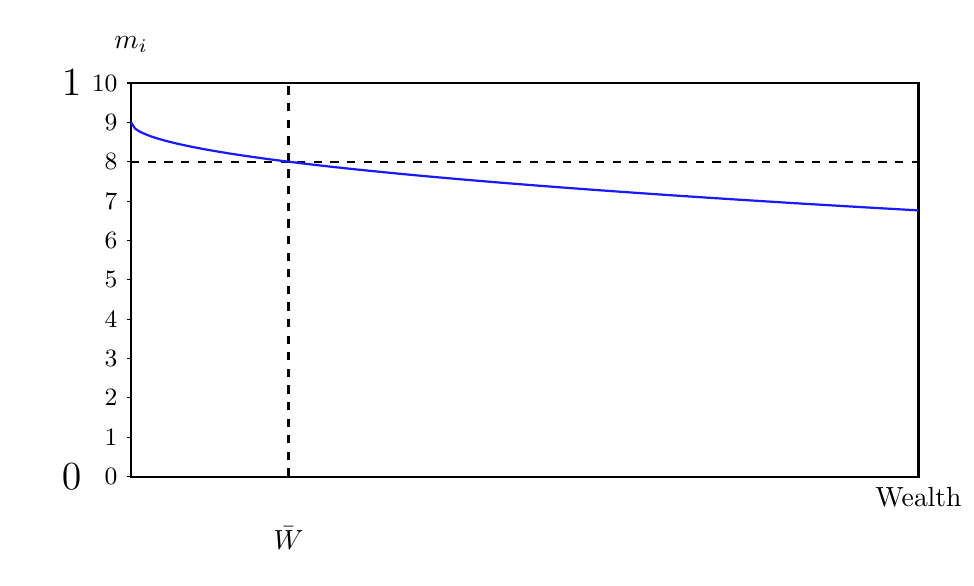
\begin{tikzpicture}[scale=.5]
%\def\bndmax{5}        %https://tex.stackexchange.com/questions/68462/filling-a-complex-region-with-tikz
%\def\bndmin{0.2}
\def\Y{10}  % height of y axis pecent
\def\W{20}  % length  of x axis
\def\Wbar{4}
\def\rbar{8}% this is the prime rate

% %Equation   \[ r_i = (A + .5 \frac{\bar{W}}{W_i})\omega\]
   % \def\Wmin{.63}  %This sets the lower limit fo the 
    \def\Wmin{(\B*\Wbar)/(\Y/\rbar-\A)} %function to keep in in bounds
	
 \tikzset{func/.style={thick,color=blue!90}}	

 \draw [thick](\W,\Y)-- (0,\Y)node[left=.5cm]{\Large$1$}node[above=.25cm]{$m_i$} -- (0,0)node[left=.5cm]{\Large$0$}--(\W,0)node[below]{Wealth}--cycle;  	% Axes box
 
 \draw [dashed, thick] (0,\rbar) -- (\W,\rbar);  	% Axes
\draw [thick,dashed] ( \Wbar,0)node[below=.5cm]{$\bar{W}$} -- (\Wbar,\Y);  	% Axes

\foreach \yi in {0,...,\Y} \draw (0,\yi)--(-.1,\yi)node[left]{\small$\yi$};
%\foreach \yi in {0,2,4,6,8,10} \draw (0,\yi)--(-.1,\yi));
%node[left]{\small$\yi$};
%\foreach \yi in {0,2,4,6,8,10}node at (-.1,yi) {{10*yi}} ;
\draw[func,domain=0:\W] plot [samples=200] (\x,(9-\x^.5/2);

 \end{tikzpicture}
\caption{Individual borrowing ratio $m_i$ as a function of wealth (in tenths)}
 \label{Fig:Borrowingratio}
\end{figure}


\subsection{Individualized borrowing rates}\label{SS:BorowingRate}
 $r_i$ 
 
 $r_i$ should depend on  both the person's income and their assets compared to others. The median after-tax income of Canadian families and unattached individuals was \$66,800 in 2020 according to Statistics Canada's \href{https://www150.statcan.gc.ca/n1/daily-quotidien/220323/dq220323a-eng.htm}{Canadian Income Survey, 2020}.  \href{https://www150.statcan.gc.ca/t1/tbl1/en/tv.action?pid=1110005501}{Data released in 2020 by Statistics Canada} indicates that the top 1\% of Canadians made, on average, around \$512,000 in a single year. \href{https://www150.statcan.gc.ca/n1/daily-quotidien/201222/dq201222b-eng.htm}{Survey of Financial Security, 2019}.

 A study by Statistics Canada found that the typical Canadian household now has a median net worth of \$329,900, while the average net worth in Canada is \$738,200. \href{https://www150.statcan.gc.ca/t1/tbl1/en/tv.action?pid=1110005501}{High income tax filers in Canada}

\subsection{Computing the income constraint on interest rates}\label{SS:YWealthConstraint}
$r_i$

In our model, we  tie the individual cost of capital,  $r_i$ for agent $i$, to a prime rate, $\bar r$ or the bank's target rate, $r^{target}$, prime plus 1\%, say. and to individual wealth. Figures~\ref{Fig:Borrowingrate1} and ref{Fig:Borrowingrate1} illustrate a couple of possible  cost-of-borrowing models roughly consistent  with the stylized facts about lenders. 

\begin{align}
 r_i =  &  \left(A + B \frac{\bar{W}}{W_i}\right) \bar r       \label{eq:incomeandr1}  \\
 r_i =  &  \left(\bar r - A + B *\frac{\bar W}{W_i - C}\right) \label{eq:incomeandr2}  \\
\end{align}
Where $\Bar{W}$ is mean wealth and $W_i$ is individual wealth. In Equation~\ref{eq:incomeandr2},  A determines y-shift, B, the scale, and C the  x-shift for the curve.


\begin{figure}
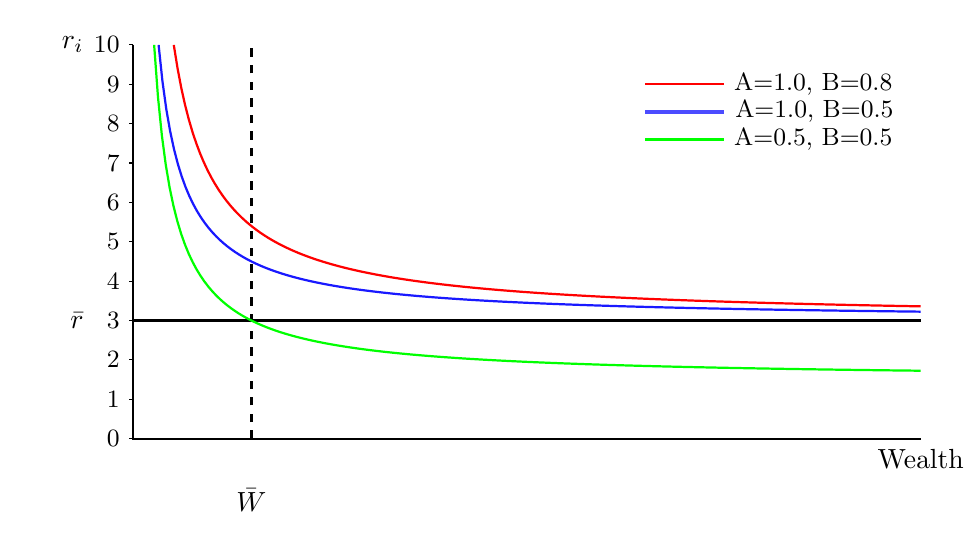
\begin{tikzpicture}[scale=.5]
%\def\bndmax{5} % https://tex.stackexchange.com/questions/68462/filling-a-complex-region-with-tikz
%\def\bndmin{0.2}
\def \Y {10}    % height of y axis as a pecent
\def \W {20}    % length  of x axis
\def \Wbar {3}  % mean wealth
\def \rbar {3}  % the prime rate 

% Equation   \[ r_i = (A + .5 \frac{\bar{W}}{W_i})\omega\]
\def \Wmin{.63}  %This sets the lower limit fo the 
\def \Wmin{(\B*\Wbar)/(\Y/\rbar-\A)} %function to keep in in bounds
\tikzset{func/.style={thick}}	

% Axes
\draw [thick] (0,\Y)node[left=.5cm]{$r_i$} -- (0,0)--(\W,0)node[below]{Wealth};  
\foreach \yi in {0,...,\Y} \draw (0,\yi)--(-.1,\yi)node[left]{\small$\yi$};
\draw [thick] (0,\rbar)node[left=.5cm]{$\bar r$} -- (\W,\rbar);  	% Axes
\draw [thick,dashed] ( \Wbar,0)node[below=.5cm]{$\bar{W}$} -- (\Wbar,\Y);  	% 

\def \A {1.0}  \def \B {0.5} %BLUE
\draw[func,domain=\Wmin:\W, color=blue!90] plot [samples=200] (\x,{(\A+\B*\Wbar/\x)*\rbar});
\draw [ultra thick, color=blue!70 ](13, 8.3)--(15,8.3)node [right, black] {\small A=\A,\ B=\B};

\def \A {0.5} 
\def \B {0.5} % GREEN
\draw[func,domain=\Wmin:\W, color=green] plot [samples=200] (\x,{(\A+\B*\Wbar/\x)*\rbar});
\draw [thick,  color=green](13, 7.6)--(15,7.6)node [right, black] {\small A=\A, B=\B};

\def \A {1.0}  \def \B {0.8} % RED
\draw[func,domain=\Wmin:\W, red] plot [samples=200] (\x,{(\A+\B*\Wbar/\x)*\rbar});
\draw [thick,  color=red](13, 9)--(15,9)node [right, black] {\small A=\A,\ B=\B};
% KEY
\end{tikzpicture}
\caption{Individual borrowing cost as a function of wealth}
\label{Fig:Borrowingrate1}
\end{figure}


\begin{figure}
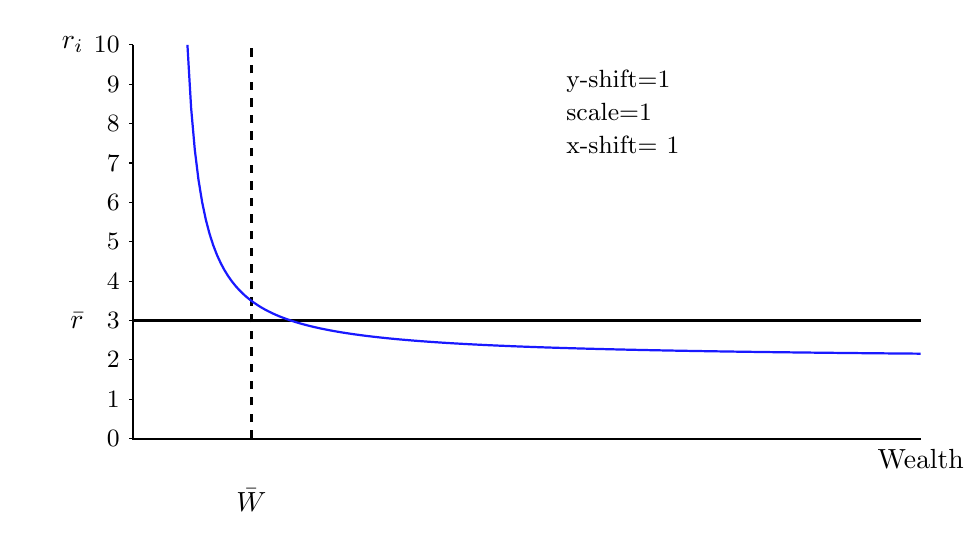
\begin{tikzpicture}[scale=.5]
%\def\bndmax{5}        %https://tex.stackexchange.com/questions/68462/filling-a-complex-region-with-tikz
%\def\bndmin{0.2}
\def \Y {10}  % height of y axis pecent
\def \W {20}  % length  of x axis
\def \Wbar {3} % meam wealth
\def \rbar {3}% this is the prime rate 

%\def \Wmin{(\B*\Wbar)/(\Y/\rbar-\A)} %function to keep in in bounds
\tikzset{func/.style={thick}}	
	% Axes
\draw [thick] (0,\Y)node[left=.5cm]{$r_i$} -- (0,0)--(\W,0)node[below]{Wealth};  
\foreach \yi in {0,...,\Y} \draw (0,\yi)--(-.1,\yi)node[left]{\small$\yi$};
\draw [thick] (0,\rbar)node[left=.5cm]{$\bar r$} -- (\W,\rbar);  	% Axes
\draw [thick,dashed] ( \Wbar,0)node[below=.5cm]{$\bar{W}$} -- (\Wbar,\Y);  	% 

\def \A {1} %vertical shift aroung \rbar, the prime rate
 \def \B {1}  % Scales the exponential curveBLUE
 \def \C {1}  %right shift  
% \def \Wmin {.4+\B}  %This sets the lower limit fo the 
\def \Wmin {(\B*\Wbar)/(\Y-\rbar+\A) +\C} %function to keep in in bounds

\draw[func,domain=\Wmin:\W, color=blue!90] plot [samples=200] (\x,{\rbar-\A+\B*\Wbar/(\x-\C))});
\node  [align=left, text width =2cm ] at (13, 8.3) {\small y-shift=\A \newline scale=\B \newline x-shift= \C};

 \end{tikzpicture}
\caption{Individual borrowing cost as a function of wealth II}
\label{Fig:Borrowingrate2}
\end{figure}

The rates $\delta,\ \sigma,$ and $r$ depend on the period, $T$. 

\section{Incorporating growth and discounting}
%We need a time period T for calculations. For use in any calculation, 

With a price-growth rate of $\dot P$ per year, the growth over $T$ years is $(1+\dot P)^T$, and  %and a 5 year mortgage period, 
the expected price at the end of the period is:

\[P^e_T=P_0(1+\dot P)^T\]

If, for example price growth is 10\%, $\dot P= 0.1$, the {capital gain}, or growth, over a 5-year mortgage term is 0.61051 $\approx$ 60\% of the original price, $P_0$.

If we want the compounded interest rate person $i$ the term T,
\[r_i^T=(1+r_i)^T\]
% This is the value we use in equation~\ref{EqBidPrice}.

If person $i$  discounts at a discount rate $r^\delta$, the present value of a receipt at time $t$ is calculated by using the \textbf{discount factor} $\delta_i^T$.

\[\delta_i^T= \left( \frac{1}{1+r_\delta} \right)^T \]
%\[\delta_i^T= \sum_{\tau=0}^{\tau=T}\left( \frac{1}{1+r_\delta} \right)^\tau \]
 
These can be combined into a function %\delta that  gives a single discounting factor  for a value  like future price that is both growing and being discounted over several (T) periods:
\[ PDV(P^e_T)=P_0\left( \frac{1+\dot P}{1+r_\delta} \right)^T \]
This PDV function specifically combines any expected rent increase, the individual's discount rate and the mortgage term into a single operation.

\subsection{Mortgage availability}
For home loans, many personal finance experts recommend total housing costs account for less than 28\% of your \textbf{gross} household income, This gives us an \textbf{income-based  mortgage maximum} of \[M^{max}_Yi = \frac{0.28*(\omega+w)}{r_i}\] It is the maximum the bank will let you pay.

We assume $r_i$ is based on the individual's assets, on relative wealth. Where is it calculated for the householder or the bank?

We get a \textbf{price-based mortgage maximum} \[M^{max}_P = 0.8P_0\] where $P_0$ is the actual sale price. This is based on the maximum amount of risk that the bank is willing to take on. ($P_0$  will not always be the same as the asking price or the warranted price.)


\section{Table}

\renewcommand{\arraystretch}{1.5}
\begin{tabular}{rlrr}\
Symbol         & Name                                 & Value      & Formula  \\ \hline
$m_i$          & Individual borrowing-ratio           & 0.75-0.85  & $M/P^{ask?}$ \\
$M^{max}_Yi$.  & Maximum mortgage based on income     &            & $\frac{0.28(\omega+w)}{r_i}$ \\
 $M^{max}_P$   & Maximum mortgage based on the price  &            & $0.8*P_0$ \\
$IS$           & Income share for housing debt        & 0.25-0.35  & Missing? \\
$\rho$         & Rent ratio                           &            & $\frac{\omega-tau*d_i}{P_0}$ \\
$\kappa $      & Operations ratio                     & 0.1-0.3    & e.g. $ 0.2\frac{\omega-tau*d_i}{P_0}$ \\
$\sigma$       & Tax ratio                            & 0.25-0.35  & e.g. $ 0.3\frac{\omega-tau*d_i}{P_0}$ \\
$\dot P $      & Price growth                         & []         & $\frac{P_t-P_{t-1}}{P_{t-1}}$\\
$P^T_e$        & Expected price in T years            &            & $P_0(1+\dot P)^T$ \\ % *** WAS $P^e_T$ 
$r_i^\delta$   & Individual discount rate             &            & To assign \\
$\bar r$       & Prime interest rate                  &            & \\
$r_i$          & Individual borrowing-rate            &            & \\
$r^{target}$   & Target interest rate                 &            & $\bar r + margin$ \\
$\delta_i$     & Discount factor for T                &            & $\left(\frac{1}{1+r_i^\delta}\right)^T$ \\
\end{tabular}
\renewcommand{\arraystretch}{1.0}


todo look for $P^e_T$ 

%==========================EXAMPLE=========================== https://www.kaggle.com/code/prateekmaj21/basic-financial-calculations-using-python/notebook
  
% def compound_interest(p,r,t):  %EXAMPLE
    
%     print('Amount: ', p)
%     print("Rate of Interest (Per Annum)", r)
%     print("Time (In Years): ",t)
    
%     a= p*((1+r/100)**t)
    
%     ci= a-p
%     print("Final Amount: ", a)
%     print("Compound Interest: ", ci)
 

\section{Transportation costs}
Transport costs have two parts:
1) fuel and vehicle costs per km
2) time costs per km

\subsection{Vehicle related costs}
Use one year as the wage period, converting transportation costs per km to annual cost for consideration in the household budget. Starting with the cost per km, calculate the cost per year:

\textbf{cost per km =$\textit{t}$}:. \$0.59   (from  Ontario data, 2021). sensitive to congestion, use of subways (\$5 /day?), 

 \textbf{work trips per year} 2 way * 5 days/week * 50 weeks work days = 500. [range: 450-550]

\textbf{cost per km-year} = work trips per year*cost per km

=\$0.59/km*500 trips/year  =  \$295/km year 



\subsection{Time costs}
\textbf{time per km}. range: 20km/hr -> 3min/km, 40km/hr -> (1.5min/km - 3min/ km)per trip 

(New York rush hour is much slower:  4-9km/hr ->6-15 min/km)

\textbf{time  per km-year} = work trips per year*time t per trip = 500* 3min  = 1500 min/km year = 25 hours= 3-3.5 days/km
 
\textbf{time cost per km-year} =  (days per km-year /work days/year)*wage premium per year  = 3/250 = 0.012 years/km year. ?

\textbf{money cost of time per km year} 

=time cost per km-year* wage(including subsistence) 

= 0.012 year* wage per year

\subsection{Total cost per km year of commuting for one agent}
\textbf{money cost of time per km year + \$295/km year * distance} \\
= (0.012 w+ \$295)/km year 
    \begin{quotation}
    \textbf{Example}
    To get a sense of the required wage if we have this annual cost structure, assume city\_extent $d^*$ is 30 km. At this point the transport cost is equal to the wage

\[(0.012 w+ \$295)/km year)*30 =  w\] 
\[.36w+ 8850=w\]
\[w=13828.12\]
        \begin{quotation}
        \textbf{PLAUSIBILITY CHECK}
This is plausible land rent, but does not include building rent. 
Capitalized at 5\% this house is worth \$ 276,562, a fairly cheap house 30 miles from city centre
        \end{quotation}
    \end{quotation}

{\color{red}
\subsection{? Value of $t$ to use in model}}
\[ \tau=(0.012 w+ \$295)/km year \]


% % \chapter{Amenity}\label{chapter-amenity}

In this chapter, we discuss how amentity might be treated in this model. 
% from Ricardo_Rent_and_Roemer_3.tex
In our base model,  an urban wage premium is the only labour attractor. Transportation costs to the urban center determine land values. Effectively in our base model, we have set the level of amenities to zero  to focus on the productivity effects. The wage premium provides a reason to find housing in the city and to travel to the city centre to work. Housing choice, however, in reality is always the purchase of a bundle of characteristics such as location, building space, yard, local density and local \glsdisp{amenity}{amenities}. Stegman  found that ``a large majority of families who have recently moved to the suburbs are more concerned with neighborhood quality than with accessibility to other parts of the metropolitan region.'' 
``There is evidence that the amenities offered by a city enhance its growth'' \cite{clarkAmenitiesDriveUrban2002, falckPhantomOperaCultural2011} and that amenity effects themselves scale superlinearly \cite{kraemerCulturalSustainabilityUS2022}.

Kaufmann et all \cite{kaufmannScalingUrbanAmenities2022} investigated the general statistical patterns in the quantity and spatial distribution of different urban amenities including public spaces and institutions as well as businesses, which all provide different services to urban populations, such as restaurants, parks, or universities.  They argue that amenities are in fact central for generating and supporting economic agglomeration effects, attracting investment to ``developing neighborhoods, promoting economic growth, supporting innovation clusters and facilitating businesses linkages.'' 
They show that the aggregate quantity of amenity infrastructure (not amenity supply)  in an urban area scales sub-linearly with population size across US metropolitan areas.\footnote{When they disaggregate, however, they find that for approximately 74\% of amenity types, they cannot reject linear scaling. Four percent exhibit super-linear scaling. They list take-away restaurants and travel agents in this range. Sub-linear scaling is associated with libraries, universities, and movie theatres.} This strongly suggests there are scale economies in amenity provision.\footnote{The model they use is the same as the one used to demonstrate that a scaling law holds for urban GDP. Instead of GDP, however, the dependent variable is a measure of amenity density based on data extracted from a unique new Google Places dataset, Google Places API (2012).} 


The amenities offered by a city can be seen as a form of non-market, non-monetary income \cite{kaufmannScalingUrbanAmenities2022}.  The non-market component of household incomes affects choices. Greater consumption amenities in a city will make workers willing to accept lower wages or higher rents. For firms,  lower wages mean lower costs. Thus,  higher amenity levels may lead to lower money wages as workers trade amenity for money income. With lower wages, more workers can be hired leading to higher output and a larger population \cite{pugaMagnitudeCausesAgglomeration2010}. 
When positive urban amenities prevail, rents and housing prices will be higher in larger cities, but wages may be unaffected \cite{robackWagesRentsAmenities1988, dalmazzoAmenitiesSkillbiasedAgglomeration2011}.
%localized productive advantages will make firms willing to accept higher wages and higher rents  


%It involves budget allocation. If we hold the housing budget constant and add an explicit urban amenity, other variables must adjust. 
% Higher wages make residents better off whereas higher rents make them worse off. Thus, 


%.  This helps disentangle the consumption amenities from the productive advantages of big cities.


In our base model,  To introduce amenities we can simply add an amenity value $A$ to the estimated value of any home. The value can depend on location, allowing for `better' and `worse' neighbourhoods,  and it can be made to depend on household attributes: a family with children might value a neighbourhood with a school or a park more highly. 

For some households, the amenity of an area may depend on the density of the city or of certain types in a neighbourhood. This is a social agglomeration effect that may work in addition to the agglomeration effect on production \cite{gurwitzCatastrophicAgglomeration2019} that we have already considered. There are also agglomeration effects in consumption goods. Larger consumer markets support more variety in goods and services. This variety allows a greater range of preferences to be satisfied. A larger city may have more production sectors and a larger array of consumer services, increasing the value received from a given income.  These closely related but different effects can be modeled by introducing an amenity term in various ways 

The amenity-induced rise in housing prices may absorb what would otherwise be consumption expenditure on other goods. Residents might accept smaller housing units for access to urban amenities.\footnote{Some costs may fall with agglomeration. There is evidence of a strong negative correlation between the total energy consumption of a city and its overall urban density \cite{newmanSustainabilityCitiesOvercoming1999}. Larson et al. \cite{larsonEnergyImplicationsCity2015} show that per-capita energy use is relatively invariant to city size when growth is driven by wages but falls modestly with growth induced by rising amenity.} In any case, there will be distributional effects as amenities play a larger role in urban agglomeration. Property owners will capture increased land rents. If amenities are funded out of taxes, the burden falls on all residents, since property taxes are very roughly related to housing consumption, but the land rents are captured by institutional owners as well as owner-occupiers and not by tenants.


%\glspl{amenity}, or non monetary income it another form of wealth,See Kaufmann et al. \cite{kaufmannScalingUrbanAmenities2022}.  and it is %, are however, an important feature of the urban system. 
% We have intentionally suppressed amenity but can add it it simply.
% (ownership effects, produtivity spilllovers, - table where you show them in the static and dynamci case with amentity)
% 2 classes of exploratin of the model in the past tho chaptered

 
%To understand amenity in our model, we need to understand it's relationship with growth, productivity, and agglomeration.
\section{Modelling amenity}

This section sketches an extension of the model to study include \gls{amenity} and suggests how it might affect results. Amenity effects can be introduced in a variety of ways. %hey might work though An economics might prefer to introduce amenity as a good in the utility function of agents.
% It might then depend on the size of the city, the size of an amenity-producing sector, the specific amenity-generating infrastructure provided by the city through taxes,  or neighbourhood effects. Each of these would take a different functional form. In our model agents are represented by their demand for housing, so the same terms would be introduced into the bid function. % In the utility framework, bids are simply derived from the utility function, so the two approaches are equivalent. %  The virtue of using the utility framework is that it begins with the question, ``What do people want?'' rather than ``What do people do?'' The first question is more productive if we want to identify different amenities that might matter.

\subsection{Through household utility}
The most direct way to incorporate agglomeration amenities is  to include what might be called a \gls{utility premium} for urban dwellers as non-monetary location income $\mathbb{A}(d; N), \die{\mathbb{A}}{N}> 0), \die[{\mathbb{A}}]{d}< 0)$ depending on distance, $d$ from the centre and urban population $N$. The second term can incorporate local amenities as well. A simple linear (indirect)\footnote{The indirect utility function is a function that depends on income and prices rather than goods and services.  Income does not generate utility, but it does generate utility indirectly' because it enables people to purchase goods and services.} utility function specified on broad income (net wage plus locational amenity) is convenient for illustration:

\begin{equation}VU(w,A)= \psi+ \omega-cd + \mathbb{A}(d; N) - T(d))
\label{eqn-u}
\end{equation}
where $w$  is an urban wage p, $T(d)$ is transportation cost from the centre to $d$.
\footnote{\cite{anasUrbanSpatialStructure1998} shows that a linear transportation cost will not  hold if congestion declines  with $d$.} 
 In most versions of the Alonzo model the `wage premium' is simply given in the urban wages and there is no amenity term. 


%\footnote{wage income, if all income goes to housing, or the share of wage income going to housing services.   (If we use a Cobb-Douglas utility function we would just replace $w$ with    $\alpha Y$, where $Y$ is household income and $\alpha$ is the share of total income. } Let  $T(d)=td$ be transportation cost with  $t>0$. 
 
\begin{figure}[t!b]
\begin{center}
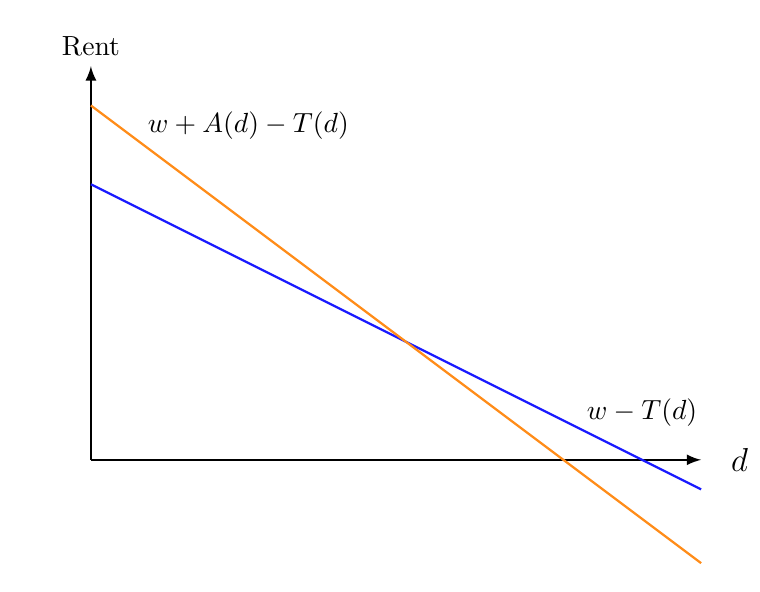
\begin{tikzpicture}[scale=.5]
\def\bndmax{5}        %https://tex.stackexchange.com/questions/68462/filling-a-complex-region-with-tikz
\def\bndmin{0.2}
\def \n {10}
\def \m {15.5}
\def \t {.5}
\def \th {1}
\def \w {7}
\tikzset{func/.style={thick,color=blue!90}}	
\draw [thick, latex-] (0,\n)node[above] {Rent}--(0,0);
\draw [thick, -latex] (0,0)--(\m,0)node[right=.25]{\large $d$};
%\foreach \xi in {0,..., \m} \draw (\xi,0)--(\xi,-.1)node[below=1]{\small$\xi$};
%\foreach \yi in {1,...,\n} \draw (0,\yi)--(-.1,\yi)node[left]{$\yi$};
%%\foreach \i in {1,4,9,16} {
	\draw[func,domain=0:\m] plot [samples=200] (\x,{\w-\t*\x});
%	\draw[func,domain=0:\m, dashed] plot [samples=200] (\x,{\w+\azero-\th*\x+\aprime*\x});

\node at (14,1.2){$w-T(d)$};
\def \azero{2}
\def \aprime {-.25}	
\tikzset{func/.style={thick,color=orange!90}}	
	\draw[func,domain=0:\m] plot [samples=200] (\x,{\w+\azero-\t*\x+\aprime*\x});
\node at (4,8.5){$w +A(d)-T(d)$};
%\node at(-.8,2) [left]{base $2^1=$};
%\node at(-.8,1) [left]{$2^0=$};
%\draw[dotted] (0,2)--(1,2)--(1,0); 
 \end{tikzpicture}
\end{center}
\caption{Rent profile with amenities}
\label{fig-amenity}
\end{figure}

 This model can produce variations on the standard result in the Alonso model. Figure~\ref{fig-amenity} illustrates a linear amenity function, $\mathbb{A}(d|N)= a-b*d$, that is convenient for illustrative purposes.  It shows how a particular amenity function might affect the rent profile, and hence city size and it allows simple experiments with the effect of increasing population on city size, wages and rents. 

In this case, amenity falls below zero in the outer regions of the city and, the geographical size of the city will be smaller. With a linear function, this happens if $\frac{a}{b} < \frac{w}{t}$. (a smaller city would have a secondary effect on wages, since with fewer workers' marginal productivity would be higher and therefore wages would rise. This would partially offset the initial decline in population.)
There would be a band of land around the city with negative amenity for commuters.\footnote{The very simple graphical result rests on several assumptions - no other housing expense, housing all the same size, wages all equal, preferences identical, transportation costs.}

The far more likely case is that $A(d) > 0$ when $w-T(d)$ falls to zero. In this case there is a band of residents around the city, outside of the population commuting to work. They do not travel to work,  do not collect a wage, but still enjoy the amenity of being close to a city. This might be a population of retired persons enjoying occasional visits and healthcare facilities.


\subsection{Neighbourhood amenity}
In Figure~{fig-amenity} the source of the amenity is at the centre of the city. We can easily imagine an amenity profile that is high for some neigbourhoods and lower for others, as in  In Figure~\ref{fig-amenity2}. The jagged area below the orange line is rent accruing to landowners. The variable rent comes not from a desire to be close to the source of the wage income but from household demand for local amenity.  
\begin{figure}[tb]
\begin{center}
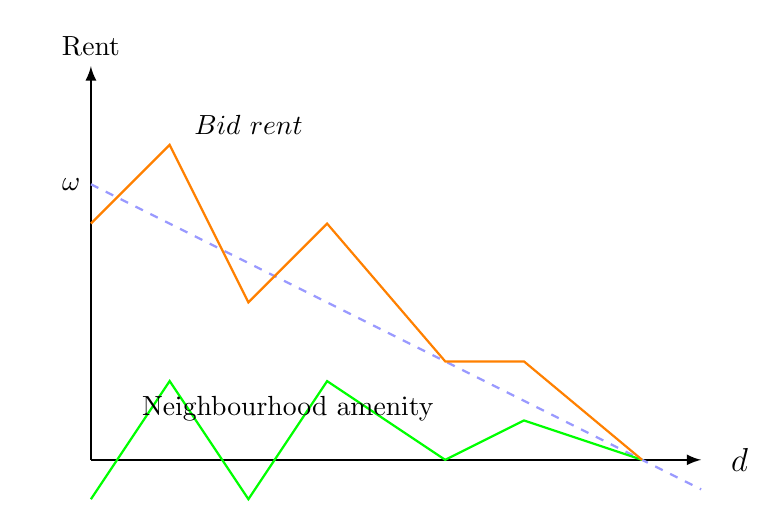
\begin{tikzpicture}[scale=.5]
\def\bndmax{5}        %https://tex.stackexchange.com/questions/68462/filling-a-complex-region-with-tikz
\def\bndmin{0.2}
\def \n {10}
\def \m {15.5}
\def \t {.5}
\def \th {1}
\def \w {7}
\tikzset{func/.style={thick,dashed, color=blue!40}}	
\draw [thick, latex-] (0,\n)node[above] {Rent}--(0,0);
\draw [thick, -latex] (0,0)--(\m,0)node[right=.25]{\large $d$};
% Basic Bid rent,
\node at(-.5,\w) {$\omega$};
\draw[func,domain=0:\m] plot [samples=200] (\x,{\w-\t*\x});
%NEIGBOURHOOD AMENITY
\draw [thick, green] (0,-1)--(2,2)--(4,-1)--(6,2)--(9,0)--(11,1)--(14,0);
\draw [thick, orange] (0,6)--(2,{7-2*.5+2})--(4,7-4*.5 -1)--(6,7-6*.5+2)--(9,7-9*.5)--(11,7-11*.5+1)--(14,7-14*.5);
\node [] at (5,1.3){Neighbourhood amenity};
\def \azero{2}
\def \aprime {-.25}	
% \tikzset{func/.style={thick,color=orange!90}}	
% 	\draw[func,domain=0:\m] plot [samples=200] (\x,{\w+\azero-\t*\x+\aprime*\x});
\node at (4,8.5){$Bid\ rent$};
%\node at(-.8,2) [left]{base $2^1=$};
%\node at(-.8,1) [left]{$2^0=$};
%\draw[dotted] (0,2)--(1,2)--(1,0); 
 \end{tikzpicture}
\end{center}
\caption{Rent profile with neighbourhood amenities}
\label{fig-amenity2}
\end{figure}
Financialization might or might not affect neighbourhood amenity. If it does it might have its effect by changing the ownership mix.

\subsection{Public provision of amenities}

Previous sections suggest amenities may work as a wage subsidy, potentially increasing output. Since employers will not willingly pay for urban amenities, some amenities may be financed publicly. It is common to introduce the cost of generating amenities as a tax on residents.  Since public amenities may be \glspl{public good} in the economic sense, the municipal government may be able to achieve significant wage economies with a small public expenditure.

A simple way to incorporate publicly provided amenities to make an amenity function that proportional to a fraction of public revenue, which is a fraction $\tau$ of the land value when municipalities depend on property taxes. Assuming a uniform property tax rate, total property tax revenue in a circular city are approximately $\tau(\phi+2/3 \omega)\pi \frac{\omega}{c}^2$. We can therefore include in the buyer's maximum bid function a fraction if this value. Property investors would not include this amenity component, but it would affect their decisions because amenity raises their net rent.

Notice that because amenity raises property values, in Ontario it does not raise tax revenue because the property tax rate is adjusted to balance the budget. This creates perverse incentives for municipalities \cite{blaisPerverseCitiesHidden2011}.


\subsection{An amenity sector}
Producing amenities takes resources. Some fraction of the workforce must be engaged in producing the amenity services. A simple approach would be to assume that the base employment that we consider demands a layer of amenities that represent the additional fraction of the population needed to provide the amenities - say 10\%  

Larger cities can support larger and more varied amenities, so that effect of amenities on property values might be larger in larger cities. At the same time, there are apparently economies of scale in the production of amenities \cite{kaufmannScalingUrbanAmenities2022}. We have no strong prior about how in amenity sector would be affected by finacialization of housing.  An effect might work through changing ownership.


\section{Research on amenities}
% There is a great deal of research on amenities. In this subsection mention a few that seemed noteworthy. 
Most of the literature on amenities deals with livability and the benefits for the individual. There is a strand in the literature, however, that links amenities to growth. In 1954, for example, Edward Ullman \cite{ullmanAmenitiesFactorRegional1954} published  ``Amenities as a Factor in Regional Growth,'' an article that came to be seen in the geographical literature over the following 50 years as prescient \cite{walcottCommentsEdwardUllman2010} for introducing the notion that amenities could be an important mobility magnet. 

Many have since extended this approach. Richard Florida, in a series of articles and books beginning in 2002 \cite{floridaCreativeClassEconomic2014, floridaEconomicGeographyTalent2002, floridaCompetingAgeTalent2005} examined the notion that urban growth depended on attracting the creative class and that in turn rested in part on the amenities a city offered. A 2008  Statistics Canada study, `Cities and Growth: The Left Brain of North American Cities,' Beckstead et al \ found substantial differences in average growth for cities with higher cultural employment and urban amenities.  Clark et al \cite{clarkAmenitiesDriveUrban2002} argue that much of Chicago's recent growth to 2003  should be attributed to reforms instituted by Mayor Richard M.  Daley explicitly linked to amenities and quality of life issues, including parks and schools. Abouy \cite{albouyWhatAreCities2016} finds that wage and housing cost differences across metropolitan areas are accounted for more by productivity than quality-of-life differences, however. 

Beckstead et al  \cite{becksteadCitiesGrowthLeft2008} identify amenities with the unexplained variastion in median urban house price after controlling for median household income.\footnote{  The basic premise would be that after conditioning on household income, variation in home prices across cities would be a function of the relative attractiveness of these places. The residuals yield a continuous ranking of cities based on the estimated variation in urban amenities.} Rappaport \cite{rappaportConsumptionAmenitiesCity2008} presents empirical evidence that amenities do support high-density levels, and that amenities cause approximately one-fifth of the cross-sectional variation in metro population density. 


% Molotch's (1976) metaphor suggests that the city is a machine geared to creating growth, with growth loosely defined as the intensification of land use and thus higher rent collections associated professional fees and locally based profits. Many urban economists, planners, and political scientists have made similar arguments (e.g., Bradbury, Downs, & Small, 1982; Mollenkopf, 1983; Stone, 1989). However, a quarter century later in the contemporary competition among US cities, the growth machine model has lost much of its power.
  


\newpage


% \chapter{Notation}
% \section{Notation for Urban and Production Sectors}
\newpage
\begin{longtable}{lp{10cm}}
\caption{Notation}                       \\
\hline           &  \textbf{Productivity} \\ \hline
$K$              &  Capital               \\ 
% $L$            &  Labour                \\
$N$              &  Population, equals labour \\ %, $L$          
%$\Lambda$    &  Labour-augmenting agglomeration effect \\
$Y=A K^{\alpha }N^{\beta }$  &  a Cobb-Douglas Production function \\ %Urban output            \\
$\alpha$         &  Elasticity of output with respect to capital          \\
$\beta$          &  Elasticity of output with respect to labour           \\ % vs effective labour
$\gamma$         &  Elasticity of agglomeration with respect to labour    \\ % , $\Lambda(n)$, for illustration \\

% $L$              &  Labour supply \\ %the number of workers, which, in the standard circular city model, equals the number of lots of size $s$  when workers live on identical individual lots. % Unless $d^{max}>d^*$ v  \frac{\pi}{s}(\frac{w}{{c}})^2 =
$n$  &  Number of workers at a firm \\
% $n_i$  &  Number of workers employed by firm $i$ \\
%$n=\sum_i n_i$  &  Number of workers, the urban population in the model \\
% $\#f=\frac{n}{n_i}$&number of identical firms \\ %not used
% $f$  &  Number of firms =1 \\
% $n =f n_i$  &  Aggregate labour \\
% $n^\gamma$ & The labour-augmenting agglomeration effect,  modelled as an exponential function of the number of people \\
% $\Lambda(n)n_i$ &  Effective labour for firm $i$ \\
% $\Lambda'=\die{\Lambda(n)}{n} $ & Derivative of the labour-augmenting agglomeration effect\\

%%$Y_i=K_i^{\alpha }(\Lambda(n)n_i)^{\beta }$  &  Urban firm $i$'s output \\

%%$Y=\frac{n}{n_i}K_i^{\alpha }(\Lambda(\sum_i n_i)n_i)^{\beta }$  &  Aggregate output of all firms in the city \\
% $\die{Y}{n}=\beta\frac{1}{n} Y  \left( 1+ \frac{n\Lambda'}{\Lambda} \right)$  &  Social marginal product of labour \\
% $Y_i=K_i^{\alpha }(\Lambda(n)n_i)^{\beta }$    &  Urban firm $i$'s output \\
% $\die{Y_i}{K_i}	=\alpha \frac{1}{K_i} Y_i $  & Marginal product of capital for firm $i$ \\
% $\die{Y_i}{n_i}	=  \beta\frac{1}{n_i} Y_i $  &  Marginal product of labour for firm $i$ \\
%%$\eta=\frac{n_i\Lambda'}{\Lambda}$  &   Marginal agglomeration effect on a firm's output of increasing it's own labour stock \\
% \hline
	% &\textbf{Amenity}\\ \hline
% $A(d, n)$   &  Agglomeration amenity          \\

\hline  0 &  \textbf{Labour market}                \\ \hline %and urban stucture??
$\psi$            &  Rural subsistence wage                             \\  
$\omega$          &  Urban wage premium          \\
${c}$             &  Transportation cost per unit distance \\ % Was $\tau$, and $trans$. Considered $\gamma, \xi, \zeta$.
$d$               &  Distance from city centre   \\
$d^* = w/{c}$     &  City extent \\ %, the maximum distance commuters will travel \\ % Maximum distance commuters will travel \\ % to get the wage premium \\
% $\mathcal{R} = \omega - {dc}$ &  Rent at distance ${d}$ \\ 
% $\zeta$          &  Population density at distance $d$     \\
% $s$              &  Lot size      \\
% $\psi$  &  ?Per-period cost of a unit of productive capital \\
% $\omega + \psi$  &  Urban wage including rural wage \\ %***
% $\textit{t}$ & {\color{red}transportation cost per km} \\%use   c?
% $w^n=\omega-{dc}$ & Wage  premium net of transportation costs \\
%% $\Omega=\frac{\omega+\psi}{\psi}$  &  Ratio of the urban wage to the  cost of capital \\
%% $\Pi$	   &  Profit \\
%% $ER$	   &  Excess return to capital \\ 
% \hline &\textbf{Spatial structure in the circular city} \\ \hline		
%% $d^{max} = \omega /{c}$  &  Maximum distance commuters at which residents enjoy the urban amenity \\
%% $d^{**} = max(d^*, d^{max})$  &  radius of the city \\
%% $U$                     &  Worker utility **\\ %, a function of location and prices \\
%% $U^{urban}=U^{rural} $  &  Migration equilibrium assumption ** \\
% \hline & \textbf{Labour market} \\ 

\hline           & \textbf{Financial market}             \\ \hline
$P_W$            &  Warranted price for a property       \\
$P_B$            &  Bid price                            \\ % was P^{bid}
$P_A$            &  Asking price                         \\
$P_M$            &  Realized market price                \\
$P_M^e$          &  Expected market price                \\
% $P$            &  Price of a property                  \\ 
% $\dot P$       &  Rate of price growth              \\ % was $\dot p$  
% $\mathcal{C}$    &  Capital gains                     \\ % was C
% $\mathcal{C}_N$  &  Net capital gain, $C -$ net rent  \\
% $M$              &  Mortgage                          \\ 
% $m$              &  Mortgage share, the share of the property price that can be borrowed, which is a function of wealth  \\ 
$\mathcal{R}$    &  Rent                              \\
$\mathcal{R}_N$  &  Net rent                          \\
${R}^w_N$        &  Warranted rent                    \\
$\rho$           &  Rent ratio                        \\
$\phi$           &  \Gls{rent share}                  \\
$\mathcal{O}$    &  Operational costs                 \\
% $\theta$         &  Operations ratio                  \\ % was $\kappa$ became b
$\mathcal{T}$    &  Taxes                             \\ % was $\Sigma, \Xi$  
$\tau$           &  Property tax share                \\ % was t then $\sigma, \xi$  b
% $\tau$            &  Annual tax rate on rent and home \\ % Was $c$ 
$r$              &  Interest rate                     \\
$\delta$         &  Individual's subjective \gls{discount factor} \\
% $W$            &  Wealth                            \\
% $\psi$         &  Fraction with rent/operating costs\\
$t$              &  Time                              \\

W & Wealth \\
m & Mortgage share \\
M & Mortgage \\
S & Savings \\
% \mathbb{C} carrying 0.28, max_mortgage share, wealth_sensitivity

$\mathbb{T}$     &  Time period                       \\

$a$       &  Share of subsistence wage  used for land and building \\
$b$       &  Maintenance share of share of subsistence wage \\ % A cost. Includes water, electricity, heat? 
% $wage_share$     & OLD Share of the agglomeration effect that goes to workers. \\

\hline
\color{black}
\end{longtable}  

\newpage

\begin{longtable}{lp{10cm}}
\caption{Rent}                                                            \\
\hline
$\omega-{dc}$                &  Warranted (economic) rent                \\
$\mathcal{R}=\omega-{dc}$    &  Equilibrium rent payment of tenant       \\
PDV                           &  Present discounted value                 \\  
$\mathcal{R}^T$               &  PDV of rent collected over period $T$    \\ 
$\mathcal{R}^T_N=(1-\kappa-\sigma)\mathcal{R}^T$  &  PDV of net rent collected over period $T$ \\
\hline
\end{longtable}

\begin{longtable}{lp{10cm}}
\caption{Bidding mechanism notation}                                          \\
\hline
$\mathcal{R}_N$  &  Net rent                                                  \\ % was NR
% $P_0$            &  Purchase price for a property                             \\
% $P^T_e$          &  Expected price at the end of period $T$                   \\
$r^{prime}$         &  Prime interest rate                                       \\
$r^{target}$     &  Investor or banks target interest rate, $\bar r + margin$ \\

$r_i$            &  Agent $i$'s personal borrowing rate                       \\
$r_i^T$          &  Agent $i$ interest rate compounded over a period $T$      \\
$r_i^{disc}$     &  Agent $i$'s subjective discount rate (which may equal $r_i$) \\
$r_\delta$       &  Discount rate                                             \\ % was $discr_i$
$\delta_i^T$     &  Discount factor for agent $i$ over period $T$             \\
$m^W$            &  Wealth-based share of home price a worker can mortgage    \\ % $= m_i(W_i)$
$m^\omega$       &  Income-based share of home price a worker can mortgage    \\ % IS_i   IS_i(\omega+\psi)$$
$m_i = min(m^W_i, m^\omega_i)$  & Mortgage, the share of home price worker $i$ can mortgage \\

\hline
\color{black}
\end{longtable}  
Notation: 
Agent counts and indices are subscripts.
Values related to time are superscripts, time as a continuous 
variable is small, a period is capitalized e.g. the period $T$ of some number of years. 
In general values are capitals, rates are small letters.

% It might be better to use the subscript $m$ for `market'.  for warranted rents



 


% Everything
\chapter[Future Work]{Future Work}
\label{appendix-future-work}



In  this chapter, we discuss potential extensions of our basic model.  Models are by nature combinatoric: every added element involves making a choice among alternative assumptions and implementations. A model incorporating in binary choices is one of an implicit family of $2^n$ alternative models. We have sharply restricted our model  in order to focus on one process of significance, financialization.  This is in part so that we can explain and justify each assumption that we use, and in part because only sharply restricted models produce understandable results. 
% Those results are condition on the specific set of assumptions to ensure that 
We have designed the model to  accommodate a range of extensions that are either theoretically or interesting or important for policy-makers. 



Figure~\ref{fig-logic-extensions} illustrates  five general types of extension. The first is to move from a static population to a model with population pressure. This appears on the left as a group of three new subroutines with connections to the elements of the model most directly affected. Some links are left out to keep the figure readable. Examples of omitted links  are the channels through which  population affects labour supply and savings.  


A second class of extension would introduce a housing production sector. This appears on the right side of of the figure linked to the banking sector. It requires adding a dynamic housing  stock. 

A third major class of extensions, separable from production is to introduce variation of housing form,  density and amenity. Zoning restrictions and building codes are related. Many questions about who gets what housing arise at this point. 

{\newpage\thispagestyle{empty}
\vspace{-1.5cm}
\begin{figure}
\vspace{-4.5cm}
\begin{adjustwidth}{-0.24\textwidth}{-0.2\textwidth}
\centering
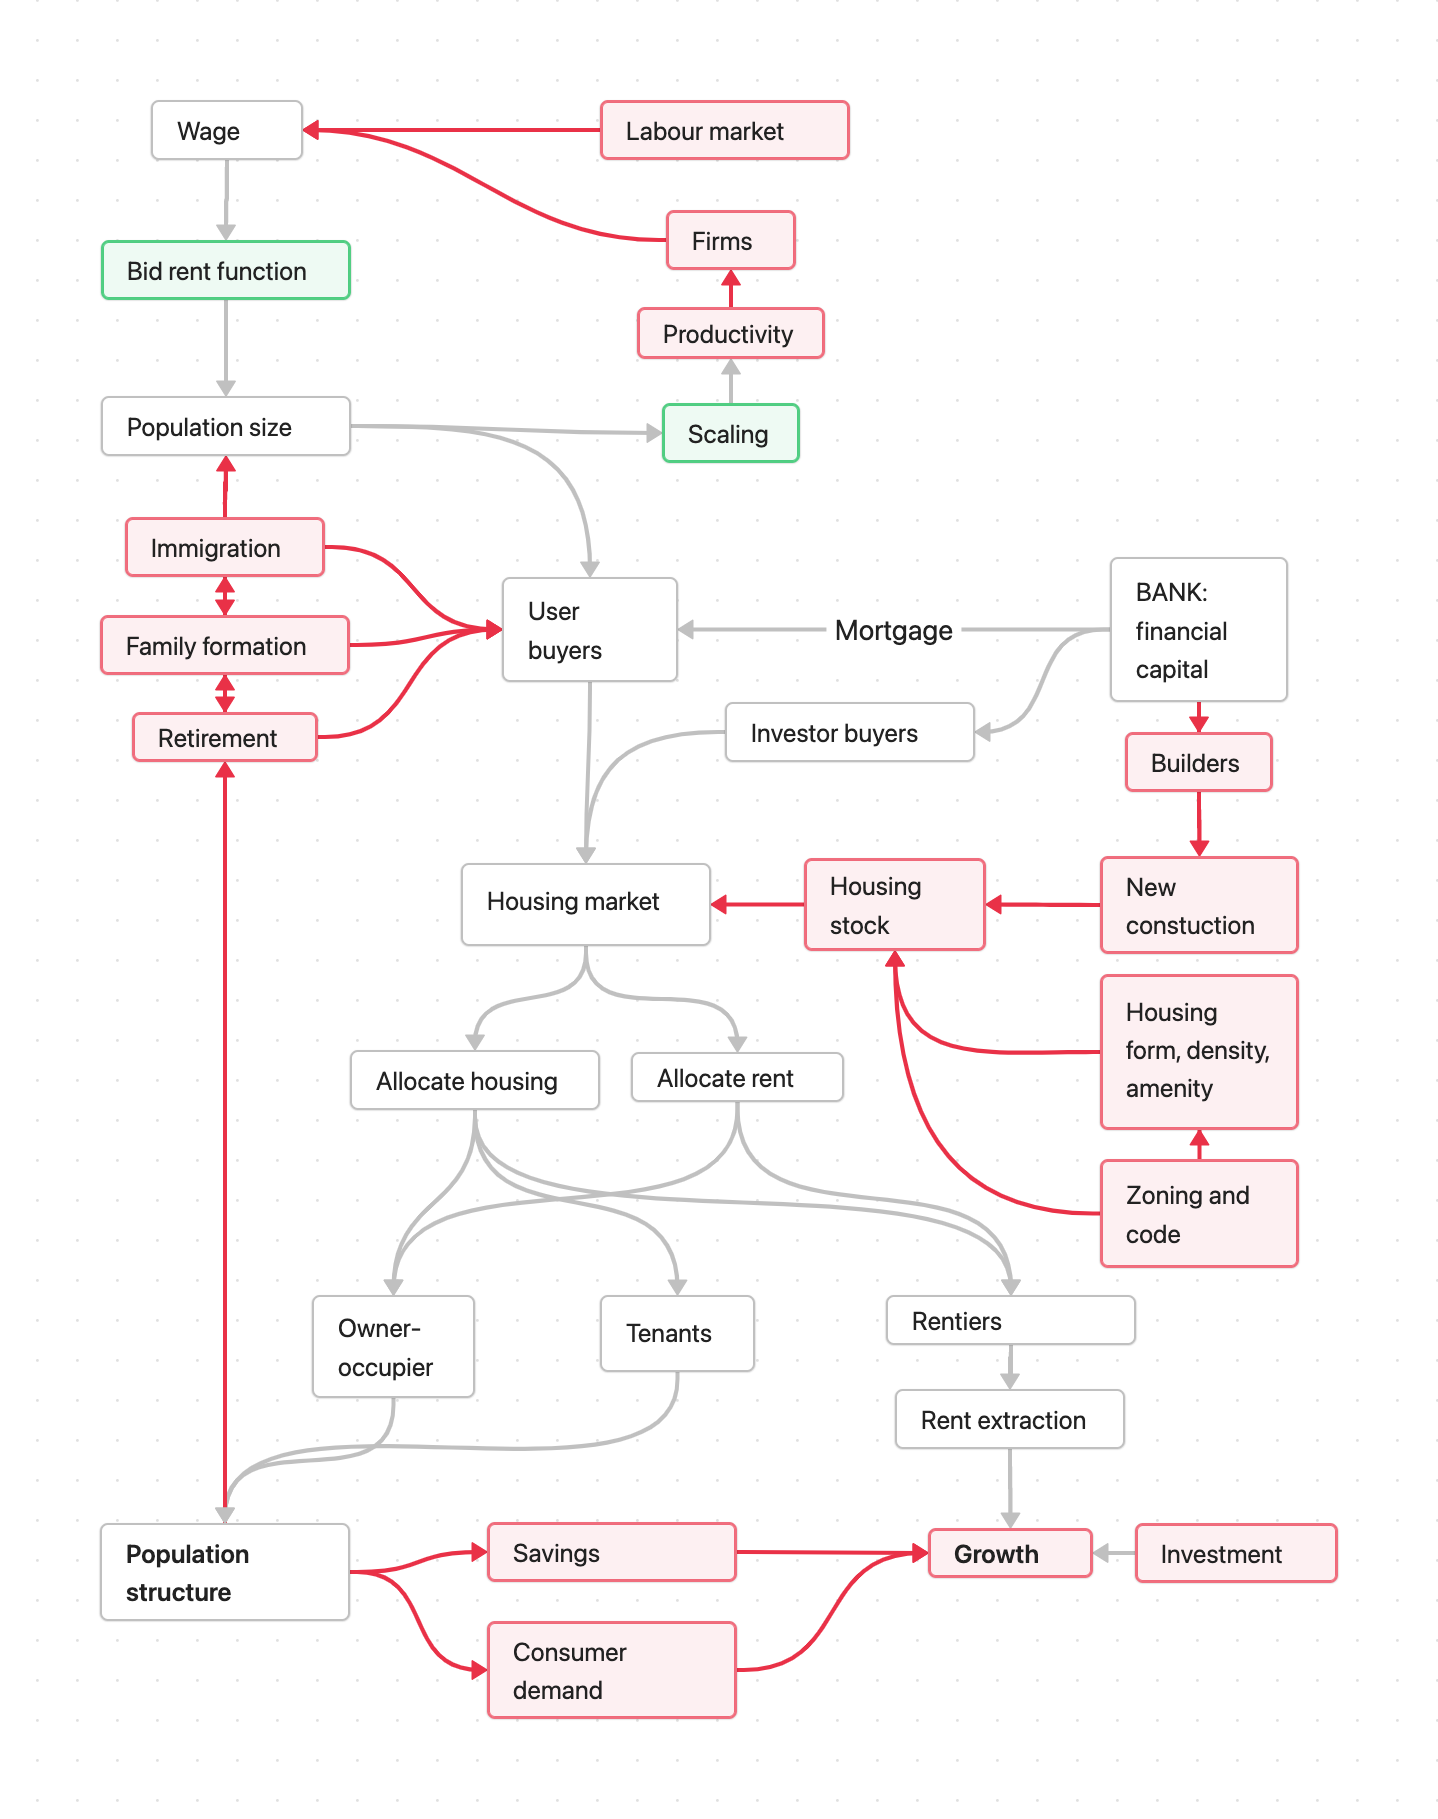
\includegraphics[scale=.22]{fig/extensions.png}
\end{adjustwidth}
\caption{Extensions}
\label{fig-logic-extensions}
%\pagestyle{headings}
% \usetikzlibrary{positioning}
%\begin{tikzpicture}[remember picture,overlay,shift={(current page.north east)}] \node[anchor=north east,xshift=-1cm,yshift=-1cm]{\includegraphics[width=1cm]{example-image-a}};\end{tikzpicture}

\end{figure}
}


At the bottom of the figure we introduce consumer demand linked to the population structure and feeding back to growth. Savings behaviour becomes more  complex when consumer demand is made endogenous and with as more complex population structure.

The fifth block of extensions illustrated in Figure~\ref{fig-logic-extensions} would replace the simple, scaling-based transmission mechanism in the Alonzo-Jacobs cycle with explicit firm and labour market behaviour. This class of extensions is obviously linked to population structure. It leads to consideration of firms that produce different products, some for export some for the local market, and to multiple types of labour.

Linked to the labour market and production system is the possibility of introducing competing cities. 

It should be clear that each of the extensions we suggest is potentially as complex as our core model, and each brings with it a collection of additional assumptions. We would argue that none of them would change our qualitative results greatly, although each would deepen our understanding of mechanisms and of the detailed impacts.


\section{Population pressure } 
Our basic model does not have a growing population. This conveniently allows us to isolate certain effects of financialization. Population pressure is one of the drivers of financialization because it amplifies speculative gains, however. As a result, one of the first extensions must be  to introduce population pressure.

There are two sources to consider: 
\begin{enumerate}
\item agglomeration effects that increase the wage and attract workers faster than the housing stock can respond. 

Worker agents from outside the city can always consider moving and accepting a job. 
% QUESTION - how to manage the flow of new agents?
%, or can make more from rents and moving away
\item immigration pressure
\end{enumerate}
under the  first, agglomeration economies drive population while under the second, population growth may drive agglomeration.

The growth of the housing stock will generally lag population growth, generating price effects and stock dynamics.

Agents will respond to increases in demand conditions. The perception that the market is tight or that prices are rising may lead to higher bids and reservation prices and shift results in favour of sellers.  


%Buyers could consider neighbourhood pressures, demographic changes, changes in job location, desire for amenity etc. in their assessment of housing need. 

%With multiple bids agents can place the most competitive bids on those homes they prefer. If they have higher urgency they place strong bids on more homes. 

%Next buyers request a selection of homes to consider from a real estate agent. Those with higher need for housing look at more homes. The real estate agent offers a selection of homes based on the agent's requirements. A randomness parameter determines how many divergent houses are also considered. When the parameter is 1, the selection of homes is fully randomized, When it is 0, the agent sorts all available homes and offers those which fit the agents budget, space, and other requirements best.


\subsection{Retirement investors and private investment properties}
The simple population turnover in our model can be replaced with a more complex set of possibilities at the agent level.  At retirement,  agents can be allowed to may choose between selling their home, renting it as an income property, or if there is sufficient amenity value for them, staying in the city. Implementing these choices complicates the agent decision and the resulting housing distribution but require few changes to the rest of the model.

\section{Housing production}

\section{Differences in density, housing form, and neighbourhood amenity}
Much of what is interesting in a city is the rich variety of housing forms and neighbourhoods and the varied populations that occupy them. Our model has a single form of housing and an undifferentiated populations, allowing us to differentiate the housing system in specific ways and study the interactions between the built world and the population. We are convinced that few of the possible extensions could affect our qualitative results. 

Nonetheless, in our agent based model, in which every lot is  addressable, it is simple to introduce zoning boundaries, local amenities, different densities or housing qualities and homes of different sizes. Hundreds of experiments are possible exploiting  the extensibility we have carefully conserved.  

We can ask what would be the effect of a hard zoning boundary and what would be the effect of suddenly relaxing it. We could explore the effect of speeding the rate of conversions from one size  home to another, or of locating high density pocket on a transportation route. Many significant urban policy questions could be examined with a limited amount of additional programming. 

\section{The consumer city}
Much of the demand for what is produced in the city is local consumer demand.  Our model has assumed there is production only for a perfectly elastic export demand. Consumer needs are buried in the subsistence wage. 

A minimal extension would be to introduce a second sector representing local consumption demand. A share of locally generated income would support production for the city's population. The labour force would be split between the two sectors and both productivity and wages might differ across sectors. 

A more complex treatment would introduce a range of service, entertainment and retail producers. This might be done monopolistically competitive firms \'a la Dixit and Stiglitz \cite{AvinashK.Dixit1977MCaO}.



\subsection{Distribution of rents}
Rents go to landowners, with a share taken for maintenance and taxes.
Rents may also be taxed, could be shared between multiple owners, etc.
 %\note{REPHRASE? rent is  extracted from the coalition of capital and workers.} % Rents may also be taxed, could be shared between multiple owners, etc. 
%The rents are captured by landowners.  The capture of rents by landowners is common buy not necessary. 
In principle the gains from urban productivity and amenity can be allocated as social wealth through shared ownership, as is often done on a small scale with cooperatives and land trusts, distributed to all citizens through something like a social wealth fund, or captured in taxes or fees as Henry George suggested. 
%The rents would otherwise go to labour and capital.





\subsection{Urban Savings - Contributions?}
THIS IS A CONTRIBUTION, BUT ALSO A DISCUSSION OF ONE WAY THIS WORK COULD BE EXTENDED, MIXED WITH A BIT OF MODEL DESCRIPTION

Conventional growth models specify a savings/investment mechanism at the national level. To our knowledge, this has not been done for the city level. We require  savings at two levels. First, since we want to incorporate  households home ownership and a relationship to the financial sector through mortgages, We specify a savings rate out of the spending we have isolated in the `subsistence wage' This means that both urban and rural workers accumulate savings, that savings are age-dependent, making the size of mortgage available also age dependent. 

Homeowners in addition have equity $E=P-M$ in their homes.  ({\color{red}Should newcomers also have equity? or is it built into the savings. Clarify this.} 

A second level of saving is the  investment in capital out of the city surplus. Even raising this question puts us into terra incognita. There are many  channels through which surplus flows into productive investment in the urban contest. One is through public investment in infrastructure. We have discussed how falling transportation costs increase surplus generation. Investments like this are made slowly and take effect over time periods much longer than our model is concerned with.  We can set a property tax rate   that we will assume is sufficient to maintain the stock of infrastructure.

Public and private investment in human capital is largely urban as well, but as with infrastructure, investment and response take effect over time periods much longer than our model is concerned with. 

Private sector innovation in technology, marketing, or products draws on local saving less but still significantly on local savings. We have little in the way of theory or empirical research on this channel. Lags between investment and any rise in the urban wage premium are almost certainly long and variable. 

We deal with this issue by linking local capital ownership with the scale factor. It is known that local ownership is associated with local investment. We will assume that local capital ownership, which consists in part of local ownership of the housing stock, can be proxied by homeowner equity as a share of local. 

\subsubsection{savings and retirement behaviour}
Agents fund their retirement from savings, as well as returns on their home if they have one to sell. Savings may be invested in a pension fund, or in local property,  depending on expected risks and returns. In the real world, financial institution manages most pensions, investing in the market or in property.  All this institutional structure is probably most easily handled by implementing a savings account for each agent. We are not interested in the detailed investment behavour for the financial sector.% either in the stock market, or in pensions.

%Institutional and individual investors can access debt. %

We could also consider a case where outside money can come under institutional management, not just local retirement savings. A parameter would control the inflow of additional money beyond local investment in the pension fund. 



\section{Making  labour market and firm behaviour explicit }
We have carefully developed the link between neoclassical growth theory and the literature on urban scaling \cite{bettencourtIntroductionUrbanScience2021} and  We then imposed the scaling result on our model.  We force the model to conform to the empirical data on the relationship between population and productivity. This amounts to black-boxing the entire production and labour demand sector as well as the construction and housing production sector. 

This made sense because our focus  was on the housing market and the financial sector, but the model we have constructed will allow us to ``fill the black box'' with more complete models of the production and labour market to see how they compare to the empirical data. 

The  scaling  literature also provides relationships between density and population and infrastructure cost and population that we can explore in the same way.

In the scaling literature, these relationships are increasingly theorized in terms of network effects, which is perfectly consistent with the Jacobs analysis and the more recent neoclassical growth modeling.


\subsection{The transmission puzzle}

The transmission of productivity increases arising from agglomeration effects  to the urban wage through firms, can be modelled in many ways. The agglomeration effects are external to the firm and therefore likely to be unexpected. If  firms underestimate the marginal product of labour, labour productivity will be greater than expected, output will be higher than planned output, and revenue and profits will therefore be higher than expected. Excess demand will attract more productive capital which in turn will demand more labour,  Rising labour demand drives up the wage. The agglomeration effect driving growth is essentially a public good in which individual firms will under-invest. This raises a policy challenge that we leave for others. CLARIFY - ALSO STILL A FOOTNOTE IN MODEL SECTION. CUT OR REF THEiR IF MOVING HERE.

 It is straightforward to compute the rate of excess return for  this model. 


\begin{figure}
    \centering
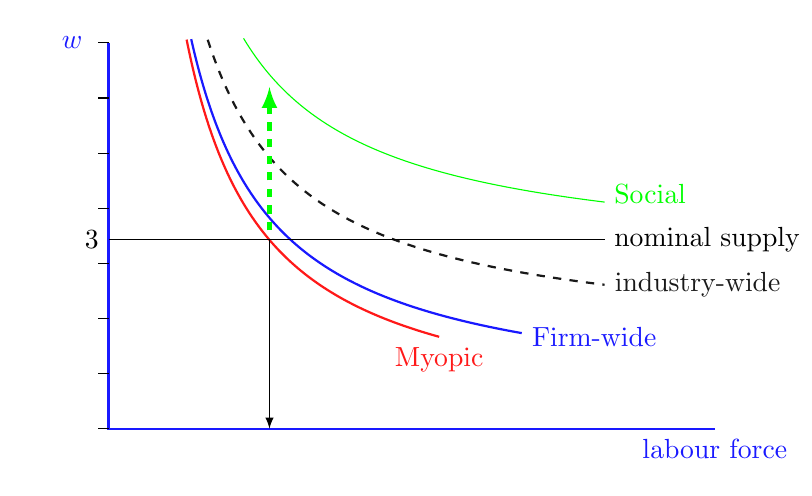
\begin{tikzpicture}[scale=.7]
%\def\bndmax{5}        %https://tex.stackexchange.com/questions/68462/filling-a-complex-region-with-tikz
%\def\bndmin{0.2}
\def \Y {7}  % height of y axis pecent
\def \W {15}  % length  of x axis
\def \Wbar {3} % jmeam wealth
\def \omega {3}
\def \A {1}  %was .5
\def \B {.5}

\draw [thick, color=blue!90] (0,\Y)node[left=.2cm]{$w$} -- (0,0)--(\W-4,0)node[below]{labour force};  
 \foreach \yi in {0,...,\Y} \draw (0,\yi)--(-.2,\yi)node[left]{};
 
\tikzset{func/.style={thick,  color=blue!90}}
% \draw[ func, domain=.2:\W-6] plot [samples=200] (\x, 2*\x^.5)node[below=.1, right]{SUPPLY};

\tikzset{func/.style={  color=green}}	
\draw[func, domain=2.45:\W-6] plot [samples=200] (\x, 10/\x+3)node[above=.1, right]{Social};

\tikzset{func/.style={thick, dashed, color=black!90}}	
\draw[func,domain=1.8:\W-6] plot [samples=200] (\x, 10/\x+1.5)node[ right]{industry-wide };

\tikzset{func/.style={thick, color=blue!90}}	
\draw[func,domain=1.5:\W-7.5] plot [samples=200] (\x, 10/\x+.4)node[below=.05, right]{Firm-wide};

\tikzset{func/.style={thick,color=red!90}}	
\draw[func,domain=8.5/6:\W-9] plot [samples=200] (\x, 10/\x)node[below]{Myopic};

\draw[](0,3.425)node[left]{$\omega$}--(9,3.425)node[right]{nominal supply };
\draw[thin,latex-](2.92,0)--(2.92,3.425); %a vertical labour supply
\draw[ultra thick,dashed, green,-latex](2.92,3.6)--(2.92,6.2);
%\draw [blue,  thick](13, 8.3)--(15,8.3)node [right, black] {\small A=\ 1,\ B=0.5};
%\draw [green, thick](13, 7.6)--(15,7.6)node [right, black] {\small A=.8, B=0.8};

%\node at (5,-1.5){Resulting in  profits, expansion, and/or entry: the city grows};
 \end{tikzpicture}
\caption{Multiple marginal products.}
\label{fig-marginal-products}
\end{figure}



Figure~\ref{fig-marginal-products} illustrates the problem. We can  make a distinction between the myopic marginal productivity curve observed by at the shop floor level and  the firm-wide effect of adding a worker. The red curve labeled ``Myopic'' represents the declining direct marginal productivity of labour as in might be observed by a shop manager, who could report how much more output one with one worker one lathe would produce. The blue line above it labeled ``Firm-wide'' represents the actual effect on firm productivity that arises because the new worker makes other workers in the firm more productive. This addition to output would be observable for managers reviewing the firm's performance over time. ' 

We can go on to consider the slower and distributed effect on closely related firms, which would raise any estimate of marginal product.  If there are 10 other firms and a new worker  has a small spillover effect  $\epsilon$ on each,  the spillovers raise the industry  marginal product  by $10\epsilon$. Each of the  10 other firms  enjoys  an additional $10\epsilon$ gain in the marginal product of their workers. This should lead to additional hiring by other firms.

Finally, expanding our view another step, we notice that if each of the  10 other firms hires one worker who produces an additional  $10\epsilon$ gain in output for all firms, the total spillover effect would rise by $100\epsilon$. The social marginal product of a single hire is indicated by the green line. 



\section{The system of cities}
Modern cities are not lonely and autarkic  beasts wandering their own exclusive territory and unconnected to others of the species. They are one is a global system of cities that compete and complement each other. Information, capital and even labour flows between cities are large. Henderson Abdel-Rahman\cite{Henderson1972Sizes}, Abdel-Rahman \cite{abdel-rahmanAgglomerationEconomiesTypes1990}, Fujita \cite{fujitaMonopolisticCompetitionModel1988}, Fujita, Krugman, and Venables \cite{fujitaSpatialEconomyCities1999}, and Fujita and Thiess \cite{fujitaEconomicsAgglomeration1996} among others provide models for expandingh the model in this direction.



\subsection{Taxes, municipal government, public goods, and productivity,}
This is a major issue with considerable development in the economics literature. Property taxes reduce the net locational value that flows to an individual owner but provides services and wages that make the city attractive. 

(create a regime where particular groups have an advantage)

Localized tax advantages can move a share of financialised investment into private consolidation of land.
including the structure of taxes for investment properties, institutional investors, individuals, etc.




\section{TO  METHODOLOGY?: Distribution}% not the right word
ABMs can be run multiple times to produce distributions of expected outcomes, which makes them valuable in planning exercises. They also do not require that we use a representative agent to make them tractable. Our model is intended to be elaborated  for such use. 

extensions
what it is
why it would be great to model
why it doesn't matter for our core results

\section{A possible typology of models and experiments}
While there  are many variations on the basic urban model and many potential experiments with each model there are only a few of immediate interest if the goal is to text the ``resilience'' of equilibria.

These models may exhibit irreversibilities in variables such as distribution, homelessness, city form, and class structure. 

The basic strategy for examining the system resilience is to shock a model (experiment) and then see if diagnostic variables recover. (This needs more precise expression.)

The first task is to select a subset of models an experiments that are of particular interests with respect to.

The second is to construct a model that allows those case to be examined. Ideally the model would be easily adapted to other experiments.

The following is a an attempt to develop a typology with a clear progressive structure.

Feedback - wealth allows upgrading. This advantages the rich. Maybe this 

\subsection{Models}
\begin{enumerate}
\item \textbf{A: The basic model}

The workhorse of urban economics is the circular city model. Some feature of the central place generates rents. It may be that it is the only employment centre. It may be economies of scale to a single activity or synergies arising from various externalities\footnote{We are interested in agglomeration economies. The wage  structure would then be related to the population or industry  structure. Externalities driving agglomeration may be classified  into two types, the  or so-called ``Marshalian''  and ``Jacobs'' externalities.}. 

In the simplest model, the central place pays a uniform wage, $w$ to all employees, who have identical preferences and transportation costs. $w$ is an attribute of individual residents. Residents  purchase or rent equal quantities of land at differing locations $l$ for identical housing.  

There are transportation costs $T$ that depend on distance from the  central place, so land close to the central place is more attractive than land farther from the central place.  

The equilibrium concept is that a market with identical individuals with identical incomes and transportation costs will result in identical utilities. The result is that land rent must decline with distance from the central place to offset rising transportation cost. 

The size of the city is determined by population and lot size. Income and transportation costs will interact with lot size. The basic model can be initialized by matching the number of properties to the size of the population. 

If population exceeds the number of properties there are three margins to consider
	\begin{enumerate}
		\item The land supply can increase. There may be a conversion cost
		\item The land per-capita may decrease. This is not simple in a city with land-use regulations, zoning, and fixed capital in homes. A conversion process has to be defined
		\item A homeless population can emerge. 
	\end{enumerate}

It is convenient in this model to use a \gls{Cobb-Douglas} utility function that has the property that a fixed fraction of income is spent on housing.  We can start with the assumption that earnings are fixed for the lifetime at the one-period wage, $w$. Then total spending on housing is $\beta Y, \beta <1$ and $ Y=w$. Let the transportation cost for a specific location $l$ be $T(l)$. The  equilibrium price at that location will be $P(l)= \beta Y-T(l)$.

It is convenient but not necessary to assume that land outside of the residential limit is costless. It is common to assume a fixed price for agricultural land. 

There is no fixed boundary and the size of the city is determined by the utility that can be achieved in competing regions of competing

\item \textbf{Y: The basic model with Income Differences}
This will result in segregation by neighbourhood depending on income. 

Income can be purely earning, which requires a distribution of $w$ across agents. Income  might include investment income, which  a private rate of return and a distribution of assets across agents. \footnote{A more subtle model could allow individual wages to be linked to the agglomeration of other workers - say engineers. we can imagine a city that has centres of agglomeration by profession or by complementarity. Depending on the production function, this should emerge endogenously.}
\footnote{Sufficient investment income could lead individuals to locate in cheap properties at the edge of the city.  Income might also be invested in property affecting the quality of a unit. This would require incorporating unit quality in the attribute list for each property, and introducing a quality preference  in the attribute s of residents.}

\item \textbf{L: The basic model with Locational Preferences}
This will result in segregation by neighbourhood depending on preferences.

One version would be include distance to the edge of the city as an amenity in the utility function. Another would be to locate amenities within the city. These would lead to higher prices near amenities.

A natural variant would be to have earning depend on location. If there were several locations  a polycentric city would emerge.

\item \textbf{T: The basic model with varied transportation cost }
This will result in segregation by neighbourhood depending on income and Transportation costs. Experiments include cars for the rich and  transit. 

Diagnostics include change in total transportation cost and differential welfare effects.

\item \textbf{R: The basic model with a rent-own choice}
This may result in the emergence of classes. Agents must have the capacity to borrow to purchase. Attributes of the agents and must now include  net assets,  an available interest rate, and a permissible mortgage.

We imagine a banker setting the mortgage rates and size. This can be done at the beginning of each period for each agent. 

With no income differential we expect equal utiliites

\item \textbf{YR: The basic model with earnings (Y) differences and a rent-own choice}
This model is likely to generate diverging classes as income differentials permit some to capture land rents from others. This is highly likely if borrowing costs decline with income and asset ownership.

\item \textbf{L: The basic model with variable lot size}
This is achieved by making lot size a choice variable for households, in which case we will get a trade off between transportation cost and lot size and distance. Results for this model are known. Density  falls with distance from the centre. 

\item \textbf{YL: The basic model with earnings (Y) differences and variable lot size}
The wealthy choose larger homes and lots farther form the centre

\item \textbf{S: The basic model with constant lot size and variable density}
This is achieved by allowing stacking of housing units. Results for this model are not known. This introduces a step change in housing form, and emphasizes unit size.

This model should produce some interesting spatial patterns, especially if couples with the possibility of secondary central places.

\item \textbf{YS: The basic model with earnings (Y) differences, constant lot size and variable density}

This model should produce some interesting spatial patterns, especially if couples with the possibility of secondary central places.

\item \textbf{IR: The basic model with outside investors and rent-own}

\item \textbf{IYR: The basic model with outside investors, earnings differentials and rent-own choice} This model is of interest if borrowing costs decline with income and asset ownership.
\end{enumerate}
\subsection{Experiments}
There are various experiments of interest. You will have to pick key ones. It is not necessary to do all of them in every model. 

	\begin{enumerate}
		\item increase population
		\item increase wage
		\item add hard boundary (limit land)
		\item Introduce differential incomes
		\item Introduce differential access to capital
	\end{enumerate}

% \newcommand{\cred}{\cellcolor{red!30}}
% \begin{table}[htp]
% \caption{Potential experiments: \textbf{Pick some}}
% \begin{center}
% \begin{tabular}{|c|c|c|c|c|c|}\hline

%   &\multicolumn{5}{c|} {experiments}\\ \cline{2-6}
% Model  &1 &2  & 4 &4  & \\ \hline
%  A& \cred& \cred  &  \cred & \cred  & \cred  \\
%  Y& \cred   & \cred   & \cred   &\cred    &\cred   \\
%  T & \cred   & \cred   & \cred   &\cred    &\cred   \\
%  R & etc &  &  &  & \\
%  L &  &  &  &  & \\
%  S&  &  &  &  & \\
%  I &  &  &  &  & \\
%  YR &  &  &  &  & \\
%  IR &  &  &  &  & \\
%   IYR&  &  &  &  & \\\hline
% \end{tabular}
% \end{center}
% \label{default}
% \end{table}%

\chapter{Future work to SORT}
model development (experiments and extensions)
interventions
theoretical development
% The urban production sector pays a wage premium $w$
%This is a convenient simplification, not a necessary feature of the model. 

The rental value of land shapes the city spatially.  

\section{Experiments with this model}
Lots of simple extensions e.g. 2 cities with immigration, differentiated labour, products, market power, neighbourhood effects (see extensions map/typology), we focus on those elements central to seeing the structure of the resilience dynamics of the wealth/housing effect. Consider adding density, to look at how it interacts with agglomeration effects. (integrating with transportation effects is neat)

\subsection{Initial state}
Basic experiments has all homes owner occupied to start. Other initial tenure mixtures are easily modelled. WHY WE MIGHT WANT TO

The basic model can be initialized by matching the number of properties to the size of the population. 

In the simplest version, firms concentrate at the city centre. Workers are spread over space and pay transportation costs to commute.

The size of the city is determined by population and lot size. Income and transportation costs will interact with lot size. 

\subsection{Parameter values}

\subsection{Analysis methods}
mapping of regimes

\subsection{Data}
incorporation of local data more carefully

\section{Extensions to the model}
The simple circular city can be extended to to produce other forms, including polycentric cities and hierarchies of cities at the cost of additional computational complexity. The simple case we examine will allows us to focus on the general, and neglected, distributional features of this class of models.

\subsection{Lags and adjustment processes}
The details of the adjustment process and the system lags are selected primarily for convenience in simulations. Real-time lags are important and complex, we explore some sensitivity results, but can explore more. 

We model a fairly short lag although in reality lags are long and variable. 

\subsection{Labour adjustment costs}

in the agent model, employees are simply laid off and seek work, so there is unemployment, but there are not \glspl{labour adjustment cost} for firms.

\subsection{Agglomeration effects, and returns to scale}
The case where there are increasing returns at the city level introduces interesting dynamics, explored in appendix CITE % 'furthur discussion' appendix.

We incorporate agglomeration effects using a Cobb Douglas formulation. This allows us to focus on the results of agglomeration in the urban system, rather than specifying the system of firms that transmit the effect. 
There are a number of other ways to study the aglomeration process in more or less explicit ways.

MOVE TO PARAMETER VALUE DISCUSSION?
The strength of the agglomeration is given by $\gamma$, thus for $\gamma=0$ there are not agglomeration effects. APPENDIX?
By definition, with one person, the agglomeration effect has no influence, $\Lambda(1)=1$,  as in the \gls{Cobb-Douglas}, and empirical urban scaling results tell us that agglomeration increases with population, following a power law distribution, so we know %$\die
FIX EQN ERROR die ${\Lambda}{n}>0$. 
%%%%%%%%%. ***WHY
If $\beta=1-\alpha$, this is a \gls{constant returns to scale} production function. Without agglomeration effects, $T(n)=1$,  Then  \textbf{$\mathbf{L(n) = T(n) n}$}  WHAT IS T, WHAT IS THIS TELLING US?
Without agglomeration effects, $\Lambda(n)=1$,  Then  \textbf{$\mathbf{L(n) = T(n) n}$} 


\subsection{Returns to scale and firm under-investment}
Each firm has \gls{decreasing returns to scale}, which means each new worker increases output by less than the previous worker did.
RETURNS TO FIRM CAN BE DECLINING WHILE RETURNS TO CITY INCREASING, THEN FIRM UNDER INVESTS
explore this in the model, see Equation~\ref{eqn-prod1}.

\begin{equation}
Y=K_i^{\alpha }(\Lambda(n)n_i)^{\beta }.
% \label{eqn-prod1}
\end{equation}

MOVE DISCUSSION HERE FOR NOW

\subsection{Heterogeneous agents}
In the simplest model, the central place pays a uniform wage premium, $w$ to all employees, who have identical preferences and transportation costs. 
The wage $w$ is an attribute of individual residents.  
It is straightforward to vary i and to vary preferences. 

relax assumptions and look at how the interaction between the production of social wealth in cities interacts with housing and the extraction of rent to drive patterns in a richer model with heterogenous agents interacting over space and time. 

- wages, skill sets

\subsection{Forward looking agents}
There are reasons to expect the results obtained with  forward-looking agents to differ substantially from those obtained with a model featuring myopic agents.\footnote{For example, Lecca et al. *** \cite{LOST-Lecca-et-al-2013}  used a stylized computational macroeconomic model applicable to a regional context to demonstrate that the assumption of myopic vs forward-looking agents yields differences in the dynamics generated by a shock perturbing the initial steady state, even though the alternative paths lead to the same long-run equilibrium.} 

\subsection{Rental bidding process}
 "Just as with prices, there is an economically \gls{warranted rent} which may differ from the \gls{market rent}. Individuals make their investment decisions on their own expectations rents. the bidding process on rental properties is abstracted in the base model. Instead of modelling the process explicitly, we make the assumption that the warranted rent is the market rent, $\mathcal{R}_W = \mathcal{R}_M$." .. could implement

\subsection{Amenity}
Notation for amenity.
There may be a band surrounding the city or persons who do not commute but enjoy urban consumption amenities. 
based on location etc

\subsection{Preferences}
A utility function/algorithm specifies agents preferences over the attributes that matter. - algorithmic continuous. lexicographic- any traits. 

\subsection{Unemployment and labour adjustment costs}
There is no unemployment. there are no labour adjustment costs for firms. ***INTERESTING TO THINK ABOUT  
when people would stop working with

 falls to subsistence wage -
 too much rent, I guess they leave, they can always move somewhere

\subsection{Moving costs}
     If there are moving costs, people can be trapped in a bad situation, incurring debt, and it can still be not worthwhile to move

\subsection{Mobility}
We could look at mobility in a more sophisticated way..
Agents enter the urban market two ways. If wages rise, agents just outside the city may become commuters. This increases population. 

When homeowners in the city retire they sell their home and move to the country. This allows them  to enjoy the capital value of their home.  They either sell their home or rent it to a new occupant. 

When  tenants in the city retire they would move to the country to enjoy lower rents. This has no effect on population. It is simplest, therefore to treat tenants as permanent residents unless we want the tenant's retirement to trigger an event like a rent increase or a decision by the owner to sell the property.

\subsection{Transportation costs}
Wage and transportation cost determine the radius of the circular city, which determines the size of the labour force which affects urban productivity. The cost of travel is therefore an important variable in the development of urban productivity. 

the transportation cost/distance relationship appears to be non-linear in many cases. While the linear model connects with the established literature, we likely want to explore the implications of more empirically grounded curve (e.g. \cite{bertaudSpatialDistributionPopulation2003}).

\subsection{Multiple firms and production structure}
The scaling result at the level of the city allows us to incorporate the effect of agglomeration in a standard \gls{circular city} model in a simple way. 

We could also explicitly model labour markets and competing firms. 

Explicitly modelling labour markets with multiple firms is a natural way to specify the model more completely, see Appendix~\ref{appendix-future-work},  but it would require introducing many ancillary assumptions and selecting among alternative models of agglomeration, when when we want to focus on distributional and growth-affecting features of the system.

For simplicity, assume firms produce a variety of perfectly substitutable commodities which are exported and locally consumed at a fixed price in a large market. 
***  Increasing product variety may produce a consumption agglomeration economies as in \cite{fujitaSpatialEconomyCities1999}.

\subsection{Market power and interchangeable goods - local markets etc}
MAKE A FOOTNOTE ON MARKET POWER AND INTERCHANGIBLE GOODS??
No externalities imperfect information etc.. ensure efficiency but aren't needed, all you need is price taking for individuals to only pay attention to their own costs and their own benefits. 

\gls{externalities}, \gls{imperfect information}, \gls{monopsony}, \gls{duopoly}, \gls{monopoly}

competitive markets many sellers, many buyers, monopoly single seller, monopsony - single buyer, intermediate cases - monopolistic competition - with some market power but not complete - duopoly- some inefficiency depending on the behavioural model because in the duopoly case they may be able to take advantage of the behaviour of buyers.

Start with perfect competition, then introduce monopolistic competition is most likely.. but it's more difficult to handle. e.g. with brand names, people have some preference for some feature of your particular good so you can price it higher even though you may loose some marginal people. Firms compete on brand name and reputation, not the pure cost effect.

In the spatial economy, goods are deferentially interchangeable. Put them on a line and firms pick a place along they line. Firms are in competition but are competing on a line-.. spatial model moved over to characteristic space..---looking at this would involve overlaying another space - the characteristic space on the physical space. .. There are also local places with local grocery stores. Polycentric stores have effectively monopolistic competition in real space. - like a named cafe downtown has the same.

\subsection{Sectors}
..


\subsection{Incomes}
In the model receive the\gls{urban wage}, which is the subsistence wage plus the urban wage premium $\psi + w$.

They may get different incomes because of firm, sector or individual increases, or particularities of the 
hiring/negotiation/wadge adjustment process, path dependency, stochasticity, etc. 
All of these factors could be explored formally in the model. %ref{rockefeller}


POOR STRUCTURALLY DISADVANTAGED HOWEVER RICH WE GET
these are averages-- some are structurally below average so some are always behind simply because of the structure of the rents claimed.. that's built in FUTURE WORK- DIFFERENT INCOMES GETS YOU THAT. 



\subsection{Hiring process and unemployment} \label{section-rockefeller}
 In our model, non-urban landowners are those who live too far from the urban job center to justify commuting.  Agents join the urban market by adding their names to the firm's list of job applicants when the rent on the marginal unit of land exceeds the transportation cost. 

adjustment speeds..
 
i(did extended modelling in the Rockefeller social innovation lab)- barriers of employment for young people seeking work
- prison records, transportation, family responsibility, bias, educational attainment, expectations of success, neighbourhood factors etc.
Could explore that kind of structure in this model

\subsection{Demographics}
Could build a population model suited to particualr data sets %\ref{section-rockefeller}

\subsection{Skills and individual productivity}
The basic model consideres a non-differentiated workforce. We can add particular skills.
Some agents can be more productive than one another

Agents may move to cities to assemble networks (model as networks)
and learn specialized skills

It can evolve over time so agents can productively over pay to  
-- getting debt/resources at key stages in a persons development to aquire property and skills is important to \gls{wealth trajectories}


\subsection{Sources of agglomeration effects}
Some of the empirically wage difference comes from the dense resources  - location of cities in good places, public investment- libraries - institutions, the network effects
some from the ability of those close to the center to simply claim a larger share of resources
some 
Some of the agglomeration wage may come from people with resources and skills disproportionately choosing cities for their amenity effect. 

We can explore different drivers in the model.


\subsection{TO METHODOLOGY: Rural market and other cities}

 To simplify analysis, we assume that land outside of the residential limit is costless, following th common practice of assuming a fixed price for agricultural land \cite{GET_fixed-price-ag-land}. 

The model is constructed so that there is neither land rent nor capitalist exploitation in the rural economy. 
This special case allows us to examine the distribution of the social surplus generated by agglomeration economies and the effect of financialization.

We could explore this

\section{Interventions: Policy and Agent Strategies}
Extended appropriately, this basic model could be used for planning.

detailed models of interventions typologies of interventions e.g. local currencies, decaying currencies, 

\subsubsection{Teaching}
could use for teaching a sequence for illustration could follow to introduce x ideas - see above. - rent, space, finance treated separately, - tool to think about their relation

productivity centered urban and spatial policy

connects with growth, economic development in real places work

\subsection{Zoning}
zoning - layers interact

\subsection{Taxes}
property taxes reduce the net locational value that flows to an owner but provides services and wages that make the city attractive. 

(create a regime where particular groups have an advantage)

Localized tax advantages can move a share of financilized investment into private consolidation of land.
including structure of taxes for investment properties, institutional investors, individuals, etc.


\subsection{Insurance, risk, and mortgage backing}

Uncertainty is a key variable.

The effects of policy are large. For example in Canada, backing mortgages is the largest fiscal investment at the national level \cite{nemtinFinancializationHousingSocial2021}.

- risks, bubbles, collapse


\subsection{Housing quality, size, subdivision}
Residents  purchase or rent equal quantities of land at differing locations %$l$ 
for identical housing.  DOWN

? More generally, if we were to introduce variations in lot size and housing types  we would want the integral of the worker density function. In our ABM version  of the model we simply count the workers within the commuter shed.

\subsection{Development and Improvements}
The supply of land at any distance from the center is inelastic. 
Its value comes from proximity to the productive urban centre, not from the value of improvements made to the property.

*** Without density, the labour supply increases with the square of the wage.  other forms..

- We have an empirical curve - gives density- simply build in

- We can .. Model a subdivision process-- urban SIM, a collaborator on the missing middle grant. - model of pro-forma and typoloties/ policies makes it possible to follow..

Some nonlinearities e.g. Some may buy land seeking to develop property in the future and let it become run down. 

We could add improvements
 or consolidation, subdivision, and development. 

% Reference sections on development which is different, and the contribution of amenity % Because supply is fixed for urban land, and the landowner has a monopoly claim on rents, the rents that can be depend on wages and amenity rather than the cost of improvements made to the property.
% The source of rents is the free gifts of nature, the coming together of people to create value in cities, and the concentration of public amenity in cities. 

\section{Theory - how to pay for innovation?}

Leaving land out, however, creates a problem in  the neoclassical growth theories we will examine below. John B. Davis \cite{davisRicardoTheoryProfit1993} noted that ``Questions arise, however, when one turns to exchange between a sector paying rent and one not.'' 
Under the assumption of perfectly competitive goods and factors markets as well as marginal productivity pricing of capital and labour, neoclassical growth requires technical change to be generated outside the model because there are no resources left to innovate if both factors of production are paid their marginal product.\footnote{This follows from Euler's theorem: if, for a given level of technology $\bar A$ output Y is produced according to a \textbf{constant returns to scale} and twice continuously differentiable function of capital and labour $F(K, L, \bar A)$, Euler's theorem implies that $F_K K + F_L L=Y$, where $F_i$ is the marginal product of factor $i$. Payments to  capital and labour take up the entire national product and no resources are left to finance the production of technology-improving innovations. are paid their marginal product.} 
If, however, land is reintroduced, as it must be in an urban model, there must be rents and there is therefore a surplus available for innovation.
\footnote{An alternative and common approach is to assume imperfect competition, which may be based on increasing returns to scale, in which case firms with market power may achieve a surplus. ``Although seldom modeled outside the monopolistic competition framework, market incompleteness and imperfect competition are central to the new growth theories'' (Gilles Duranton, Growth and imperfect competition on factor markets: Increasing returns and distribution, European Economic Review, 44-2, 2000, 255-280), Similarly, Sjak Smulders and Theo van de Klundert conclude that ``Growth is higher in a more concentrated market provided that market power of firms is not too high,'' (Imperfect competition, concentration and growth with firm-specific R \& D, European Economic Review, 39-1, 1995,139-160).}



\section{SORT Rough Notes}
what does a speculative over investment.  in housing  do? - hollowed out store front

who carries what risks- banks vs individuals

subdivision and density

multiple cities,
linear cities

differential skills and wages,
work from home

details of typologies, transportation networks, etc

- make it available as a part for other models, use other models in this model


 

\subsection{Implications}
\subsubsection{Agglomeration driven under-investment}

\chapter[Model Implementation]{Model Implementation}
\label{appendix-model-implementation}

\section{Urban wage premium}

$\omega$ is the urban wage premium. It is a share of the urban agglomeration effect. 

I think of this as worker income, $\psi + \omega + r_prime*savings$ 

The wage income  $\psi + \omega$ part has to be related to the marginal productivity of workers. The urban output function from Lobo et al \cite{loboUrbanScalingProduction2013} is  
\begin{equation}Y=AN^\beta\label{LoboEqn2}\end{equation}

Where $\beta$  is the scaling exponent, with a value of,  for example, 1.13  \`a la 
Lobo. $A$ is called the ``scale factor.''\footnote{Much of the analysis assumes scale invariance of  $A$.}  The \textbf{total urban marginal productivity of a worker} is  
\[UMPL=\beta AN^{\beta-1}=\frac{\beta Y}{N} =\]
This is not the same as the \textbf{firm-level marginal productivity of a worker}. The worker total share in Lobo et al. is \[W= (1-\alpha)Y \] 
so the individual share, which should be the competitive wage, is
\[W= \frac{(1-\alpha)Y}{N} \] 
where $(1-\alpha)=0.8$ is a common estimate. If we assume that this sets the rural wage,$\phi$, then $\omega$ has to come out of the  urban surplus per worker,

\[surp= \frac{\beta -(1-\alpha)Y}{N} \] 

 so set a fraction $\lambda$ of the surplus a, and 
 \[\omega= \lambda\frac{\beta -(1-\alpha)Y}{N}= (1.13-.8) \frac{Y}{N} \] 

 Since capital expects 0.2 as its payment and labor 0.8, the surplus available to share has to be taken out of the 0.13. The easiest formulation then is probably 
 \[\omega= \lambda(\beta -1) \frac{Y}{N} =\lambda(\beta -1) \frac{AN^\beta}{N} \] 
 

$(\beta -1)$ is agglom and  $\lambda(\beta -1)$ is the workers' share of the surplus over and above the \gls{constant returns to scale} (CRS) case.   $\lambda(\beta -1)$ is 

\begin{lstlisting}
# Firm step function updates wage, omega
def step(self):
    prefactor  = self.model.prefactor
    agglom     = self.model.agglomeration_ratio
    population = self.model.agglomeration_population
    wage_share = self.model.wage_share  
    wage_premium = wage_share * (agglom-1) * prefactor * population**agglom # omega
    self.wage = wage_premium + self.model.psi
    # k thought # self.wage_premium = (wage_share * prefactor * population**agglom)/ population # omega    
    # note surplus is: (beta - 1) * (prefactor * population**agglom)
\end{lstlisting}

Where wage share is a parameter input to the model.

\section{Bidding}
\subsection{Subjective discounting}
\begin{lstlisting}
def get_discounting(self):
    """
    Delta is the subjective individual discount factor for agent
    after one year. This will be close to ri
    A factor may be a compounded rate.
    It is the present value of one dollar in one year 
    Turns one dollar in one period into dollars of present value.
    sum_delta is sum of the infinite series 
    minus discounted infinite series after mortgage_period years
    It is the present value of annual payments from one to 
    mortgage_period years e.g. of mortgage payments or rent received
    delta_mortgage_period was called   delta_period_T
    """
    
    delta = self.r_prime # if constant 
    delta_period_1 = 1 / (1 + delta) 
    delta_mortgage_period = delta_period_1**self.mortgage_period
    sum_delta = delta_mortgage_period * (1 - delta_mortgage_period)
    # Note delta_mortgage_period is subtracted to subtract the long tail
    return sum_delta
\end{lstlisting}

Delta could also depend on wealth. For example,  use the bank rate, which is the rational rate but people who are poor typically have higher rates.  It would not change as the central bank changes r-pirme
% delta could be wealth based typically higher for poor.

\begin{lstlisting}
# A version with delta depending on wealth
wealth = self.wealth
delta =
\end{lstlisting}
 
\subsection{Maintenance costs}
\begin{lstlisting}
    def get_maintenance(self):
        """Maintenance share of property service (a*b*psi summed and discounted)
        OR IS IT TOTAL maintenance COST OVER THE MORTGAGE PERIOD?
        """
        a   = self.housing_services_share
        b   = self.maintenance_share
        psi = self.subsistence_wage
        sum_delta = self.sum_delta # CALCULATE PER PERSON
        return (a * b * psi) * sum_delta
\end{lstlisting}

\subsection{Taxes}
\begin{lstlisting}
    def get_tax(self):
        """ 
        THIS DOES NOT CHANGE WITH INCREASING WAGES?
        BUT THAT IS THE MAIN WAY TO FUND A CITY

        WHAT TO CALL THIS WEHRE DOES IT GO. WHERE DO WE USE THIS VS TAU
        Just for initialization? - warranted price. 
        Use warranted prices as initialization
        Tax costs for the mortgage period, T. 
        (Example of rate for an  multiperiod annual rate)
        tax_T= tau*(omega-c*d + a*psi) * sum_delta_T
        This is assuming taxes are paid at the end of each year for T years
        tau_T       = tau * sum_T_delta 
        #  present value of the tax rate over T years        
        """
        tau   = self.model.property_tax_annually
        omega = self.firm.wage_premium # FIXED
        psi   = self.model.subsistence_wage
        a     = self.model.housing_services_share
        c     = self.model.transport_cost_per_dist # RENAME
        d     = self.distance_from_center
        sum_delta = self.model.sum_delta # TODO - make individual  - this would have to be average discounting - THIS TAKE SUM DELTA OUT - AND PUT WITH LARGER CALCULATION.. - CACLULATE FOR A PERSON/PROPERTY COMBINATION..
        return tau * (omega - c*d + a*psi) * sum_delta
\end{lstlisting}


\subsection{TODO Warranted price}
\begin{lstlisting}
@property
def warranted_price(self):
    # USELESS PLACEHOLDER - GET CALCULATION
    return self.model.firm.wage/(self.transport_cost + 1) 
\end{lstlisting}

\subsection{TODO Maximum mortgage calculation}

\textbf{wealth-based  mortgage maximum} 
 \[max\ m_i = 9-\left(\frac{W_i}{\bar W}\right)^{0.1} \]

% **Source**: Ch:model line 580, page 87.. I have done some fiddling Wealth $W_i = P-M+S.  for i - real estate agents estimated price wealth of a property owner as assessed by the bank

\textbf{income-based  mortgage maximum} of 

\[M^{max}_Yi = \frac{0.28*(\omega+w)}{r_i}\] It is the maximum the bank will let you pay.

\textbf{Combined  mortgage maximum}
\[ M_i^Y{max} = min \{9-\left(\frac{W_i}{\bar W}\right)^{0.1}P,  \frac{0.28*(\omega+w)}{r_i} \}\]

\begin{lstlisting}
# Max mortgage
wealth = property_value - mortgage + savings
mean_weath = sum(wealth)/number_of_people

def get_max_mortgage(self, applicant):
    max_mortgage =  ...
    
    return max_mortgage
\end{lstlisting}

% wealth = property_value + 
wealth $W_i = P_e-M+S$.  

- Also need mean wealth. $\bar W$ , which you have to calculate from the sums for property values total mortgages issued, and individual savings. The bank could keep these values
- Individual borrowing rate 
$r_i = (A + B \frac{\bar{W}}{W_i})\bar r=(.1 + B \frac{\bar{W}}{W_i})\bar r$.
The value .1 can be seen as the bank's share of the prime rate set by the Bank of Canada. this is an easy place to insert that value. We should discuss this detail. An alternative is
$r_i = (0 + B \frac{\bar{W}}{W_i})(\bar r_i+ bank\ margin)$.

- Maximum M  from wealth constraint = $(9-(W_i/\bar W)^{0.1}P$
  Check if $(W_i/\bar W)0.9P$ will work. 
- Maximum M  from income = $M^{max}_Yi = \frac{0.28*(\omega+w)}{r_i}$ 
% - Maximum M  $M= min(0.28*(omega+phi)/r_i,  0.8P$,  (9-(W_i/\bar W)^{0.1}P,  \frac{0.28*(\omega+w)}{r_i}   } $


 
\subsection{Net rent based on}
Tenant willing to pay, vs what it is worth for a company to buy a property.

\begin{lstlisting}
def get_net_rent(self, property):
    """Compute the rent for a land parcel, or what someone could afford
    to pay to live there. 

    Rent depends on the urban wage premium over and above the subsistence
    wage, and on transportation costs and the distance to the
    central business district. Applies with a single wage. Adjust for
    differential urban wages.

    :param property: the land parcel to get rent information for.
    """
    a     = self.model.housing_services_share
    b     = self.model.maintenance_share
    c     = self.model.transport_cost_per_dist # RENAME
    d     = property.distance_from_center 
    tau   = self.model.property_tax_annually 
    # property_tax_rate # IS THIS FOR THE MORTGAGE PERIOD
    psi   = self.model.subsistence_wage
    omega = self.model.workers_share
    return omega - c*d - a*psi - b*a*psi - tau*a*psi
    # urban_wage = self.model.firm.wage
\end{lstlisting}


\subsection{Net rent based on ..}

\begin{lstlisting}
def get_net_rent(self, property):
    """Compute the rent for a land parcel, or what someone could afford
    to pay to live there. 

    Rent depends on the urban wage premium over and above the subsistence
    wage, and on transportation costs and the distance to the
    central business district. Applies with a single wage. Adjust for
    differential urban wages.

    :param property: the land parcel to get rent information for.
    """
    a     = self.model.housing_services_share
    b     = self.model.maintenance_share
    c     = self.model.transport_cost_per_dist # RENAME
    d     = property.distance_from_center 
    tau   = self.model.property_tax_annually 
    # property_tax_rate # IS THIS FOR THE MORTGAGE PERIOD
    psi   = self.model.subsistence_wage
    omega = self.model.workers_share
    return omega - c*d - a*psi - b*a*psi - tau*a*psi
    # urban_wage = self.model.firm.wage
\end{lstlisting}

\subsection{Max Bid}

Calculate max desired bid for an agent
\begin{lstlisting}
    def get_max_bid(self, property, bidder):
        net_rent = self.get_net_rent(property)
        r        = self.model.r_prime   
        r_target = r + self.model.r_premium
        m        = 0.8 # TODO FIX - ADD WEALTH
        # I can't do delta_T. It reads as delta_transpose to me.
        sum_delta    = self.model.sum_delta 
        p_dot    = 0.01 # TODO - estimate rate of price change
        return net_rent/((1 - m)*r_target - sum_delta*(1 + p_dot - (1 + r)*m))
\end{lstlisting}

Agent will bid the min of the desired bid or the max allowed mortgage
\begin{lstlisting}
max_mortgage = self.bank.get_max_mortgage(self)
min_downpayment = self.bank.min_down_payment_share * max_mortgage
downpayment = min(min_downpayment, self.savings)
max_allowed_bid = max_mortgage + downpayment
for sale_property in (self.model.realtor.sale_listing):
    # max_bid = self.bank.get_max_bid(sale_property, self)
    # TODO Fix
    max_desired_bid = self.model.bank.get_max_bid(sale_property, self)
    max_bid = min(max_allowed_bid, max_desired_bid)
\end{lstlisting}

\section{Negotiation Process}

Bidding.

There is a problem in that they bid on all properties as a short cut. If the number of bids structures the negotiation process, we need to limit their bids or do something much more iterative. (see above section)




\section{Individual Accounting}

\begin{lstlisting}
# FIX - NEED TO ADD THIS
# Update savings
self.savings += self.model.savings_per_step

# TODO pay costs for any properties owned
# if self.residence in self.properties_owned:
#     # TODO pay mortgage if needed pay costs
#     pass
# else:
#     self.savings -= self.rent # TODO check this is right rent
\end{lstlisting}
\chapter[Parameters]{Computing Bid Price Parameters}
\label{AppendixParemeters}

% \section{Relating the bid price parameters to the code}
The bid price is: 
\begin{align}
P^{bid} \ge   \frac{ \mathcal{R}_N}{(1-m)r^{target}-\left[ \delta(1+L(P)- (1+r)m)\right]}. \nonumber
\end{align}
In the following sections, we discuss each of the terms and how they are implemented in the code. Sections are numbered: 
\begin{align}
\frac{\ref{SS:NetRent}} {(1-\ref{SS:BorrowingRatio})\ref{SS:targetr}-
\left[ \ref{SS:discountfactor}(1+\ref{SS:PriceForecast}- (1+\ref{SS:BankRate})\ref{SS:YWealthConstraint})\right]} \nonumber
\end{align}

\section{Net rent}\label{SS:NetRent}

$\mathcal{R}_N = \phi \mathcal{R}$


Where the \gls{rent share}, phi is a fraction
$\phi = (rent-taxes-costs) /rent$ 

There's a distinction between the warranted rent, the net rent, and the rent that's actually charged.



We assume that the  rent  actually charged to a tenant is the warranted economic rent, ($\mathcal{R}= \omega - \tau d_j$), but the relevant term to enter into the calculation of return on investment is the net rent $\mathcal{R}_N$ for a given property, because the returns are the returns an investor can get after paying taxes and operating costs.

In our computational model, we do the calculation in terms of a mortgage, so we want the total returns after expenses, in present value, compounded over the mortgage  period.
% We want the total returns after expenses, in present value, compounded over a 5 year period.


\begin{align}
\mathcal{R}_N &= \mathcal{R} - \Theta - \Sigma 
\end{align}


In terms of the warranted rent, 
\begin{align}
\mathcal{R}_N &= (1-\kappa_j - \sigma_j)(\omega - \tau d_j)
\end{align}

% $\mathcal{R}_N = (1-\kappa_j - \sigma_j) (\omega - \tau d_j)$

% {\color{red}
% Notice that  we need here is really the fraction of the warranted rent that the owner gets to keep after maintenance costs and taxes. It is possible that the owner is charging more or less than the economic  rent, but economic rent can be seen as an equilibrium value. Economic rent is $\mathcal{R}$.  This is (tautologically) related to the price as a fraction of the actual sale price: COULD MOVE TO THE CHAPTER NOW SINCE THE THE SECTION IS MOVED THER
% }

% \[\mathcal{R}= \frac{\mathcal{R}}{P_0}P_0 \]



If we want to know the  present value  of the \textbf{net rent}, $\mathcal{R}_N$  collect over the period  $T$, $\mathcal{R}_N^T$, we \textbf{add up} the discounted rents for each year. We may assume the rents are rising at and that the first is the current warranted rent, which gives us a computational formula. 
\[\mathcal{R}_N^T= (\omega-\tau*d)\sum_{t=0}^{t=T-1} \frac{(1+\dot{\mathcal{R}})^{t}} {(1+r_{r_\delta})^{t+1}} \]


% \[\mathcal{R}_Nj^T= (\omega-\tau*d_j)\sum_{\tau=0}^{\tau=T-1}\left[\frac{1+\dot{\mathcal{R}}}{1+r_{r_\delta}}\right]^\tau \]
\noindent where $\dot{\mathcal{R}}$ is an expected rate of change of rents - possibly zero for now, and $r_\delta$ is the individual's discount rate. 

TODO: problem - how to handle subscripts with net rent $\mathcal{R}_N$



\subsection{Target interest rate}\label{SS:targetr}

 The target interest rate, $r^{target}$, is the prime rate plus a margin. % required by the bank.  Question: do non-bank actors have such a term?

\begin{verbatim}
self.get-target-interest-rate(buyer)
\end{verbatim}


\subsection{Tax ratio}\label{SS:taxratio} 
The tax ratio $\sigma$ is the share of rents that the municipality takes for services and infrastructure. This fraction of the value of the property is about 30\% based on mill rates in Ontario,  so $\sigma = 0.3$. % REFERENCE

*** CHECK Total taxes paid on  property $j$, over a given mortgage period $T$ is 

\[\Psi_j^T = \psi * \mathcal{R}\].  


\subsection{Cost tax ratio}\label{SS:costratio} 
The value of $\kappa$  varies for every property based on maintenance requirements, historic rents, tenant rights, and variations in assessed values. If it varies, it may be useful as a quality indicator.

%Values for $\kappa$ and $\sigma$ must be adjusted to take into account the length of the period or net rents have to be summed over the period.  NO LONGER NEEDED 

Nothing prevents $\sigma+\kappa >1$, which would leave an investor unable to cover building maintenance and taxes out of current rent. 


\subsection{Discount factor}\label{SS:discountfactor}

The discount factor $\delta_i$ for THE END OF period $T$ captures the cost of waiting $T$ periods to sell the property. The usual way to treat it, which we use here, is to assume that $i$ has an interest rate $r_i$ and has been investing efficiently. This means that  the individual has a discount factor for future returns based on the year-over-year rate of return. 

\[\delta^T_i=\left[\frac{1}{1+r_i}\right]^T\]


\subsection{Price forecast approximation} \label{SS:PriceForecast}
$L(p)$

$p$ is all the price data plus any exogenous information (EG Policy knowledge?). $L(p)$ is an estimation function that produces a `common knowledge' value for the rate of price increase. Later you can add idiosyncratic extra knowledge or extra ignorance.




\subsection{Prime interest rate}\label{SS:BankRate}
$r$

The bank's interest rate, $r$, is just the bank rate (prime rate? set by the Bank of Canada. Exogenous. Just assign  a value like 4\%.


\subsection{Borrowing ratio}\label{SS:BorrowingRatio}
$m_i$

The borrowing ratio, $m_i$, is just the fraction of the price that the bank will lend to a potential buyer. \textbf{It may depend on the individual.} 

Income(\ref{SS:YWealthConstraint}) and/or wealth (\ref {SS:MWealthConstraint}) may constrain individual participation in markets. 
Here we should use the same logic as we use about the interest rate charged. (\ref{SS:BorowingRate})


It is likely to be higher for institutional buyers  and for rich people because the bank thinks rich people are more secure risks. they may have other assets that could be attached in the case of default.

\subsection{Wealth constraint on m} \label{SS:MWealthConstraint}


I have suggested that the availability of  capital is known to differ for rich and poor. 
The bank, as a person has lots of assets, so $m_i$ is close to one, say 0.9. 

For the median wealth holder, $m_i$ should be around - let's say, 0.8 and  
We need a function that captures this relationship so we need to define individual wealth:
\[W_i= P_i -M_i  +S_i\]
where 

\begin{tabular}{ll}
$P_i$ & value of owned home\\
$M_i$ & Mortgage on owned home\\
$S_i$ & personal savings = $age*d*W$\\
\end{tabular}


We first tie the borrowing \textbf{ratio}, $m_i$,  for agent $i$, to individual wealth. Figure~\ref{Fig:Borrowingratio} illustrates a mortgage availability  model that is written 
 \[ m_i = 0.1(9-\left(\frac{W_i}{\bar W}\right)^{0.5}/2 )\]
Where $\bar{W}$ is mean wealth and $W_i$ is individual wealth. 

\begin{figure}[htb]
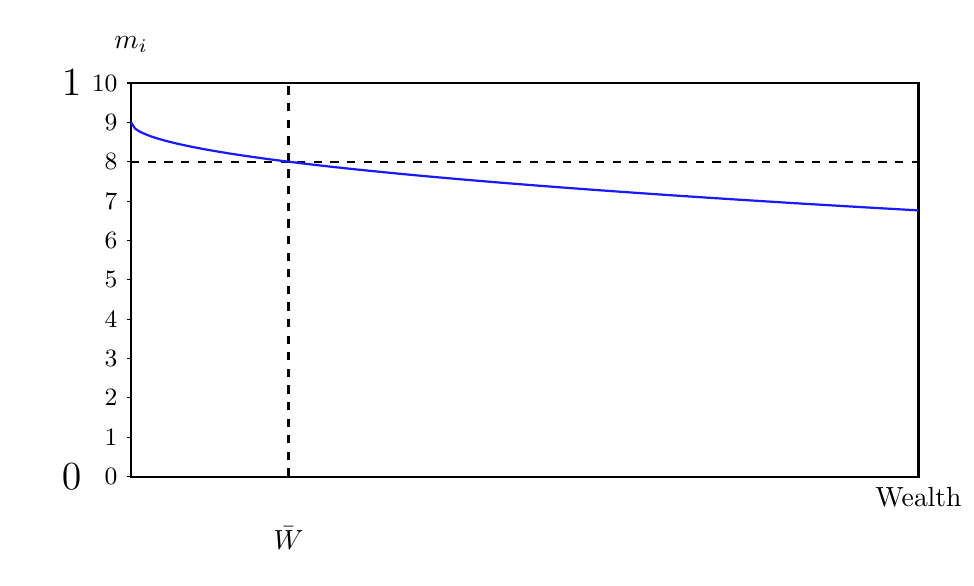
\begin{tikzpicture}[scale=.5]
%\def\bndmax{5}        %https://tex.stackexchange.com/questions/68462/filling-a-complex-region-with-tikz
%\def\bndmin{0.2}
\def\Y{10}  % height of y axis pecent
\def\W{20}  % length  of x axis
\def\Wbar{4}
\def\rbar{8}% this is the prime rate

% %Equation   \[ r_i = (A + .5 \frac{\bar{W}}{W_i})\omega\]
   % \def\Wmin{.63}  %This sets the lower limit fo the 
    \def\Wmin{(\B*\Wbar)/(\Y/\rbar-\A)} %function to keep in in bounds
	
 \tikzset{func/.style={thick,color=blue!90}}	

 \draw [thick](\W,\Y)-- (0,\Y)node[left=.5cm]{\Large$1$}node[above=.25cm]{$m_i$} -- (0,0)node[left=.5cm]{\Large$0$}--(\W,0)node[below]{Wealth}--cycle;  	% Axes box
 
 \draw [dashed, thick] (0,\rbar) -- (\W,\rbar);  	% Axes
\draw [thick,dashed] ( \Wbar,0)node[below=.5cm]{$\bar{W}$} -- (\Wbar,\Y);  	% Axes

\foreach \yi in {0,...,\Y} \draw (0,\yi)--(-.1,\yi)node[left]{\small$\yi$};
%\foreach \yi in {0,2,4,6,8,10} \draw (0,\yi)--(-.1,\yi));
%node[left]{\small$\yi$};
%\foreach \yi in {0,2,4,6,8,10}node at (-.1,yi) {{10*yi}} ;
\draw[func,domain=0:\W] plot [samples=200] (\x,(9-\x^.5/2);

 \end{tikzpicture}
\caption{Individual borrowing ratio $m_i$ as a function of wealth (in tenths)}
 \label{Fig:Borrowingratio}
\end{figure}


\subsection{Individualized borrowing rates}\label{SS:BorowingRate}
 $r_i$ 
 
 $r_i$ should depend on  both the person's income and their assets compared to others. The median after-tax income of Canadian families and unattached individuals was \$66,800 in 2020 according to Statistics Canada's \href{https://www150.statcan.gc.ca/n1/daily-quotidien/220323/dq220323a-eng.htm}{Canadian Income Survey, 2020}.  \href{https://www150.statcan.gc.ca/t1/tbl1/en/tv.action?pid=1110005501}{Data released in 2020 by Statistics Canada} indicates that the top 1\% of Canadians made, on average, around \$512,000 in a single year. \href{https://www150.statcan.gc.ca/n1/daily-quotidien/201222/dq201222b-eng.htm}{Survey of Financial Security, 2019}.

 A study by Statistics Canada found that the typical Canadian household now has a median net worth of \$329,900, while the average net worth in Canada is \$738,200. \href{https://www150.statcan.gc.ca/t1/tbl1/en/tv.action?pid=1110005501}{High income tax filers in Canada}

\subsection{Computing the income constraint on interest rates}\label{SS:YWealthConstraint}
$r_i$

In our model, we  tie the individual cost of capital,  $r_i$ for agent $i$, to a prime rate, $\bar r$ or the bank's target rate, $r^{target}$, prime plus 1\%, say. and to individual wealth. Figures~\ref{Fig:Borrowingrate1} and ref{Fig:Borrowingrate1} illustrate a couple of possible  cost-of-borrowing models roughly consistent  with the stylized facts about lenders. 

\begin{align}
 r_i =  &  \left(A + B \frac{\bar{W}}{W_i}\right) \bar r       \label{eq:incomeandr1}  \\
 r_i =  &  \left(\bar r - A + B *\frac{\bar W}{W_i - C}\right) \label{eq:incomeandr2}  \\
\end{align}
Where $\Bar{W}$ is mean wealth and $W_i$ is individual wealth. In Equation~\ref{eq:incomeandr2},  A determines y-shift, B, the scale, and C the  x-shift for the curve.


\begin{figure}
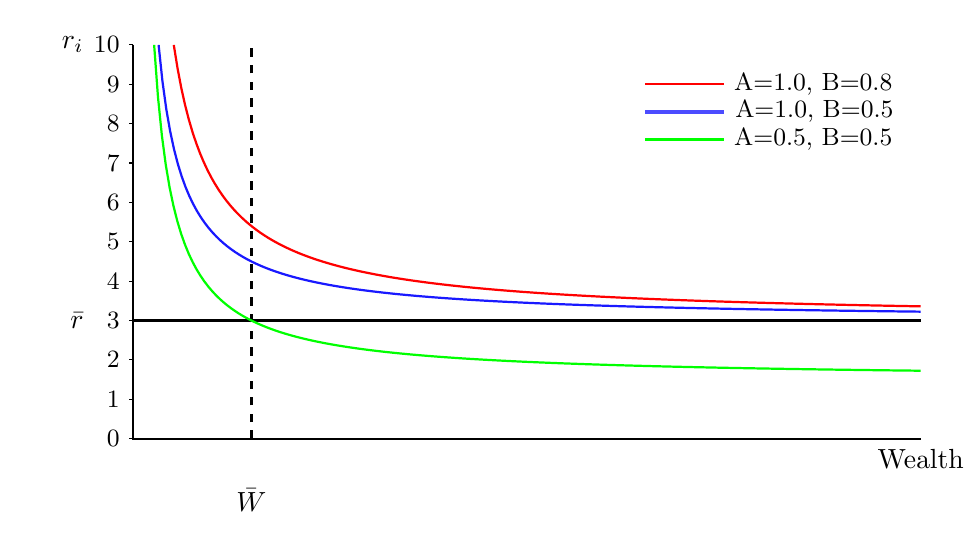
\begin{tikzpicture}[scale=.5]
%\def\bndmax{5} % https://tex.stackexchange.com/questions/68462/filling-a-complex-region-with-tikz
%\def\bndmin{0.2}
\def \Y {10}    % height of y axis as a pecent
\def \W {20}    % length  of x axis
\def \Wbar {3}  % mean wealth
\def \rbar {3}  % the prime rate 

% Equation   \[ r_i = (A + .5 \frac{\bar{W}}{W_i})\omega\]
\def \Wmin{.63}  %This sets the lower limit fo the 
\def \Wmin{(\B*\Wbar)/(\Y/\rbar-\A)} %function to keep in in bounds
\tikzset{func/.style={thick}}	

% Axes
\draw [thick] (0,\Y)node[left=.5cm]{$r_i$} -- (0,0)--(\W,0)node[below]{Wealth};  
\foreach \yi in {0,...,\Y} \draw (0,\yi)--(-.1,\yi)node[left]{\small$\yi$};
\draw [thick] (0,\rbar)node[left=.5cm]{$\bar r$} -- (\W,\rbar);  	% Axes
\draw [thick,dashed] ( \Wbar,0)node[below=.5cm]{$\bar{W}$} -- (\Wbar,\Y);  	% 

\def \A {1.0}  \def \B {0.5} %BLUE
\draw[func,domain=\Wmin:\W, color=blue!90] plot [samples=200] (\x,{(\A+\B*\Wbar/\x)*\rbar});
\draw [ultra thick, color=blue!70 ](13, 8.3)--(15,8.3)node [right, black] {\small A=\A,\ B=\B};

\def \A {0.5} 
\def \B {0.5} % GREEN
\draw[func,domain=\Wmin:\W, color=green] plot [samples=200] (\x,{(\A+\B*\Wbar/\x)*\rbar});
\draw [thick,  color=green](13, 7.6)--(15,7.6)node [right, black] {\small A=\A, B=\B};

\def \A {1.0}  \def \B {0.8} % RED
\draw[func,domain=\Wmin:\W, red] plot [samples=200] (\x,{(\A+\B*\Wbar/\x)*\rbar});
\draw [thick,  color=red](13, 9)--(15,9)node [right, black] {\small A=\A,\ B=\B};
% KEY
\end{tikzpicture}
\caption{Individual borrowing cost as a function of wealth}
\label{Fig:Borrowingrate1}
\end{figure}


\begin{figure}
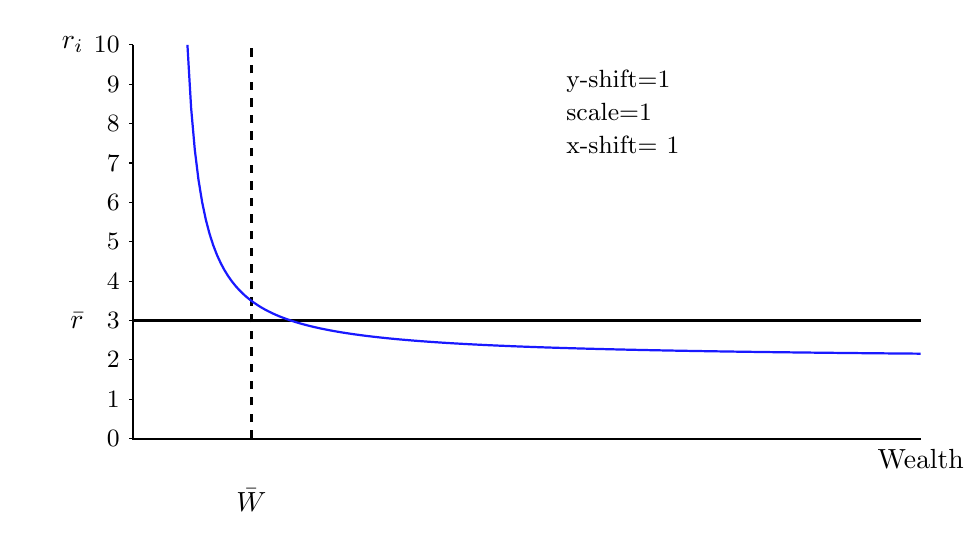
\begin{tikzpicture}[scale=.5]
%\def\bndmax{5}        %https://tex.stackexchange.com/questions/68462/filling-a-complex-region-with-tikz
%\def\bndmin{0.2}
\def \Y {10}  % height of y axis pecent
\def \W {20}  % length  of x axis
\def \Wbar {3} % meam wealth
\def \rbar {3}% this is the prime rate 

%\def \Wmin{(\B*\Wbar)/(\Y/\rbar-\A)} %function to keep in in bounds
\tikzset{func/.style={thick}}	
	% Axes
\draw [thick] (0,\Y)node[left=.5cm]{$r_i$} -- (0,0)--(\W,0)node[below]{Wealth};  
\foreach \yi in {0,...,\Y} \draw (0,\yi)--(-.1,\yi)node[left]{\small$\yi$};
\draw [thick] (0,\rbar)node[left=.5cm]{$\bar r$} -- (\W,\rbar);  	% Axes
\draw [thick,dashed] ( \Wbar,0)node[below=.5cm]{$\bar{W}$} -- (\Wbar,\Y);  	% 

\def \A {1} %vertical shift aroung \rbar, the prime rate
 \def \B {1}  % Scales the exponential curveBLUE
 \def \C {1}  %right shift  
% \def \Wmin {.4+\B}  %This sets the lower limit fo the 
\def \Wmin {(\B*\Wbar)/(\Y-\rbar+\A) +\C} %function to keep in in bounds

\draw[func,domain=\Wmin:\W, color=blue!90] plot [samples=200] (\x,{\rbar-\A+\B*\Wbar/(\x-\C))});
\node  [align=left, text width =2cm ] at (13, 8.3) {\small y-shift=\A \newline scale=\B \newline x-shift= \C};

 \end{tikzpicture}
\caption{Individual borrowing cost as a function of wealth II}
\label{Fig:Borrowingrate2}
\end{figure}

The rates $\delta,\ \sigma,$ and $r$ depend on the period, $T$. 

\section{Incorporating growth and discounting}
%We need a time period T for calculations. For use in any calculation, 

With a price-growth rate of $\dot P$ per year, the growth over $T$ years is $(1+\dot P)^T$, and  %and a 5 year mortgage period, 
the expected price at the end of the period is:

\[P^e_T=P_0(1+\dot P)^T\]

If, for example price growth is 10\%, $\dot P= 0.1$, the {capital gain}, or growth, over a 5-year mortgage term is 0.61051 $\approx$ 60\% of the original price, $P_0$.

If we want the compounded interest rate person $i$ the term T,
\[r_i^T=(1+r_i)^T\]
% This is the value we use in equation~\ref{EqBidPrice}.

If person $i$  discounts at a discount rate $r^\delta$, the present value of a receipt at time $t$ is calculated by using the \textbf{discount factor} $\delta_i^T$.

\[\delta_i^T= \left( \frac{1}{1+r_\delta} \right)^T \]
%\[\delta_i^T= \sum_{\tau=0}^{\tau=T}\left( \frac{1}{1+r_\delta} \right)^\tau \]
 
These can be combined into a function %\delta that  gives a single discounting factor  for a value  like future price that is both growing and being discounted over several (T) periods:
\[ PDV(P^e_T)=P_0\left( \frac{1+\dot P}{1+r_\delta} \right)^T \]
This PDV function specifically combines any expected rent increase, the individual's discount rate and the mortgage term into a single operation.

\subsection{Mortgage availability}
For home loans, many personal finance experts recommend total housing costs account for less than 28\% of your \textbf{gross} household income, This gives us an \textbf{income-based  mortgage maximum} of \[M^{max}_Yi = \frac{0.28*(\omega+w)}{r_i}\] It is the maximum the bank will let you pay.

We assume $r_i$ is based on the individual's assets, on relative wealth. Where is it calculated for the householder or the bank?

We get a \textbf{price-based mortgage maximum} \[M^{max}_P = 0.8P_0\] where $P_0$ is the actual sale price. This is based on the maximum amount of risk that the bank is willing to take on. ($P_0$  will not always be the same as the asking price or the warranted price.)


\section{Table}

\renewcommand{\arraystretch}{1.5}
\begin{tabular}{rlrr}\
Symbol         & Name                                 & Value      & Formula  \\ \hline
$m_i$          & Individual borrowing-ratio           & 0.75-0.85  & $M/P^{ask?}$ \\
$M^{max}_Yi$.  & Maximum mortgage based on income     &            & $\frac{0.28(\omega+w)}{r_i}$ \\
 $M^{max}_P$   & Maximum mortgage based on the price  &            & $0.8*P_0$ \\
$IS$           & Income share for housing debt        & 0.25-0.35  & Missing? \\
$\rho$         & Rent ratio                           &            & $\frac{\omega-tau*d_i}{P_0}$ \\
$\kappa $      & Operations ratio                     & 0.1-0.3    & e.g. $ 0.2\frac{\omega-tau*d_i}{P_0}$ \\
$\sigma$       & Tax ratio                            & 0.25-0.35  & e.g. $ 0.3\frac{\omega-tau*d_i}{P_0}$ \\
$\dot P $      & Price growth                         & []         & $\frac{P_t-P_{t-1}}{P_{t-1}}$\\
$P^T_e$        & Expected price in T years            &            & $P_0(1+\dot P)^T$ \\ % *** WAS $P^e_T$ 
$r_i^\delta$   & Individual discount rate             &            & To assign \\
$\bar r$       & Prime interest rate                  &            & \\
$r_i$          & Individual borrowing-rate            &            & \\
$r^{target}$   & Target interest rate                 &            & $\bar r + margin$ \\
$\delta_i$     & Discount factor for T                &            & $\left(\frac{1}{1+r_i^\delta}\right)^T$ \\
\end{tabular}
\renewcommand{\arraystretch}{1.0}


todo look for $P^e_T$ 

%==========================EXAMPLE=========================== https://www.kaggle.com/code/prateekmaj21/basic-financial-calculations-using-python/notebook
  
% def compound_interest(p,r,t):  %EXAMPLE
    
%     print('Amount: ', p)
%     print("Rate of Interest (Per Annum)", r)
%     print("Time (In Years): ",t)
    
%     a= p*((1+r/100)**t)
    
%     ci= a-p
%     print("Final Amount: ", a)
%     print("Compound Interest: ", ci)
 

\section{Transportation costs}
Transport costs have two parts:
1) fuel and vehicle costs per km
2) time costs per km

\subsection{Vehicle related costs}
Use one year as the wage period, converting transportation costs per km to annual cost for consideration in the household budget. Starting with the cost per km, calculate the cost per year:

\textbf{cost per km =$\textit{t}$}:. \$0.59   (from  Ontario data, 2021). sensitive to congestion, use of subways (\$5 /day?), 

 \textbf{work trips per year} 2 way * 5 days/week * 50 weeks work days = 500. [range: 450-550]

\textbf{cost per km-year} = work trips per year*cost per km

=\$0.59/km*500 trips/year  =  \$295/km year 



\subsection{Time costs}
\textbf{time per km}. range: 20km/hr -> 3min/km, 40km/hr -> (1.5min/km - 3min/ km)per trip 

(New York rush hour is much slower:  4-9km/hr ->6-15 min/km)

\textbf{time  per km-year} = work trips per year*time t per trip = 500* 3min  = 1500 min/km year = 25 hours= 3-3.5 days/km
 
\textbf{time cost per km-year} =  (days per km-year /work days/year)*wage premium per year  = 3/250 = 0.012 years/km year. ?

\textbf{money cost of time per km year} 

=time cost per km-year* wage(including subsistence) 

= 0.012 year* wage per year

\subsection{Total cost per km year of commuting for one agent}
\textbf{money cost of time per km year + \$295/km year * distance} \\
= (0.012 w+ \$295)/km year 
    \begin{quotation}
    \textbf{Example}
    To get a sense of the required wage if we have this annual cost structure, assume city\_extent $d^*$ is 30 km. At this point the transport cost is equal to the wage

\[(0.012 w+ \$295)/km year)*30 =  w\] 
\[.36w+ 8850=w\]
\[w=13828.12\]
        \begin{quotation}
        \textbf{PLAUSIBILITY CHECK}
This is plausible land rent, but does not include building rent. 
Capitalized at 5\% this house is worth \$ 276,562, a fairly cheap house 30 miles from city centre
        \end{quotation}
    \end{quotation}

{\color{red}
\subsection{? Value of $t$ to use in model}}
\[ \tau=(0.012 w+ \$295)/km year \]


\chapter{Amenity}\label{chapter-amenity}

In this chapter, we discuss how amentity might be treated in this model. 
% from Ricardo_Rent_and_Roemer_3.tex
In our base model,  an urban wage premium is the only labour attractor. Transportation costs to the urban center determine land values. Effectively in our base model, we have set the level of amenities to zero  to focus on the productivity effects. The wage premium provides a reason to find housing in the city and to travel to the city centre to work. Housing choice, however, in reality is always the purchase of a bundle of characteristics such as location, building space, yard, local density and local \glsdisp{amenity}{amenities}. Stegman  found that ``a large majority of families who have recently moved to the suburbs are more concerned with neighborhood quality than with accessibility to other parts of the metropolitan region.'' 
``There is evidence that the amenities offered by a city enhance its growth'' \cite{clarkAmenitiesDriveUrban2002, falckPhantomOperaCultural2011} and that amenity effects themselves scale superlinearly \cite{kraemerCulturalSustainabilityUS2022}.

Kaufmann et all \cite{kaufmannScalingUrbanAmenities2022} investigated the general statistical patterns in the quantity and spatial distribution of different urban amenities including public spaces and institutions as well as businesses, which all provide different services to urban populations, such as restaurants, parks, or universities.  They argue that amenities are in fact central for generating and supporting economic agglomeration effects, attracting investment to ``developing neighborhoods, promoting economic growth, supporting innovation clusters and facilitating businesses linkages.'' 
They show that the aggregate quantity of amenity infrastructure (not amenity supply)  in an urban area scales sub-linearly with population size across US metropolitan areas.\footnote{When they disaggregate, however, they find that for approximately 74\% of amenity types, they cannot reject linear scaling. Four percent exhibit super-linear scaling. They list take-away restaurants and travel agents in this range. Sub-linear scaling is associated with libraries, universities, and movie theatres.} This strongly suggests there are scale economies in amenity provision.\footnote{The model they use is the same as the one used to demonstrate that a scaling law holds for urban GDP. Instead of GDP, however, the dependent variable is a measure of amenity density based on data extracted from a unique new Google Places dataset, Google Places API (2012).} 


The amenities offered by a city can be seen as a form of non-market, non-monetary income \cite{kaufmannScalingUrbanAmenities2022}.  The non-market component of household incomes affects choices. Greater consumption amenities in a city will make workers willing to accept lower wages or higher rents. For firms,  lower wages mean lower costs. Thus,  higher amenity levels may lead to lower money wages as workers trade amenity for money income. With lower wages, more workers can be hired leading to higher output and a larger population \cite{pugaMagnitudeCausesAgglomeration2010}. 
When positive urban amenities prevail, rents and housing prices will be higher in larger cities, but wages may be unaffected \cite{robackWagesRentsAmenities1988, dalmazzoAmenitiesSkillbiasedAgglomeration2011}.
%localized productive advantages will make firms willing to accept higher wages and higher rents  


%It involves budget allocation. If we hold the housing budget constant and add an explicit urban amenity, other variables must adjust. 
% Higher wages make residents better off whereas higher rents make them worse off. Thus, 


%.  This helps disentangle the consumption amenities from the productive advantages of big cities.


In our base model,  To introduce amenities we can simply add an amenity value $A$ to the estimated value of any home. The value can depend on location, allowing for `better' and `worse' neighbourhoods,  and it can be made to depend on household attributes: a family with children might value a neighbourhood with a school or a park more highly. 

For some households, the amenity of an area may depend on the density of the city or of certain types in a neighbourhood. This is a social agglomeration effect that may work in addition to the agglomeration effect on production \cite{gurwitzCatastrophicAgglomeration2019} that we have already considered. There are also agglomeration effects in consumption goods. Larger consumer markets support more variety in goods and services. This variety allows a greater range of preferences to be satisfied. A larger city may have more production sectors and a larger array of consumer services, increasing the value received from a given income.  These closely related but different effects can be modeled by introducing an amenity term in various ways 

The amenity-induced rise in housing prices may absorb what would otherwise be consumption expenditure on other goods. Residents might accept smaller housing units for access to urban amenities.\footnote{Some costs may fall with agglomeration. There is evidence of a strong negative correlation between the total energy consumption of a city and its overall urban density \cite{newmanSustainabilityCitiesOvercoming1999}. Larson et al. \cite{larsonEnergyImplicationsCity2015} show that per-capita energy use is relatively invariant to city size when growth is driven by wages but falls modestly with growth induced by rising amenity.} In any case, there will be distributional effects as amenities play a larger role in urban agglomeration. Property owners will capture increased land rents. If amenities are funded out of taxes, the burden falls on all residents, since property taxes are very roughly related to housing consumption, but the land rents are captured by institutional owners as well as owner-occupiers and not by tenants.


%\glspl{amenity}, or non monetary income it another form of wealth,See Kaufmann et al. \cite{kaufmannScalingUrbanAmenities2022}.  and it is %, are however, an important feature of the urban system. 
% We have intentionally suppressed amenity but can add it it simply.
% (ownership effects, produtivity spilllovers, - table where you show them in the static and dynamci case with amentity)
% 2 classes of exploratin of the model in the past tho chaptered

 
%To understand amenity in our model, we need to understand it's relationship with growth, productivity, and agglomeration.
\section{Modelling amenity}

This section sketches an extension of the model to study include \gls{amenity} and suggests how it might affect results. Amenity effects can be introduced in a variety of ways. %hey might work though An economics might prefer to introduce amenity as a good in the utility function of agents.
% It might then depend on the size of the city, the size of an amenity-producing sector, the specific amenity-generating infrastructure provided by the city through taxes,  or neighbourhood effects. Each of these would take a different functional form. In our model agents are represented by their demand for housing, so the same terms would be introduced into the bid function. % In the utility framework, bids are simply derived from the utility function, so the two approaches are equivalent. %  The virtue of using the utility framework is that it begins with the question, ``What do people want?'' rather than ``What do people do?'' The first question is more productive if we want to identify different amenities that might matter.

\subsection{Through household utility}
The most direct way to incorporate agglomeration amenities is  to include what might be called a \gls{utility premium} for urban dwellers as non-monetary location income $\mathbb{A}(d; N), \die{\mathbb{A}}{N}> 0), \die[{\mathbb{A}}]{d}< 0)$ depending on distance, $d$ from the centre and urban population $N$. The second term can incorporate local amenities as well. A simple linear (indirect)\footnote{The indirect utility function is a function that depends on income and prices rather than goods and services.  Income does not generate utility, but it does generate utility indirectly' because it enables people to purchase goods and services.} utility function specified on broad income (net wage plus locational amenity) is convenient for illustration:

\begin{equation}VU(w,A)= \psi+ \omega-cd + \mathbb{A}(d; N) - T(d))
\label{eqn-u}
\end{equation}
where $w$  is an urban wage p, $T(d)$ is transportation cost from the centre to $d$.
\footnote{\cite{anasUrbanSpatialStructure1998} shows that a linear transportation cost will not  hold if congestion declines  with $d$.} 
 In most versions of the Alonzo model the `wage premium' is simply given in the urban wages and there is no amenity term. 


%\footnote{wage income, if all income goes to housing, or the share of wage income going to housing services.   (If we use a Cobb-Douglas utility function we would just replace $w$ with    $\alpha Y$, where $Y$ is household income and $\alpha$ is the share of total income. } Let  $T(d)=td$ be transportation cost with  $t>0$. 
 
\begin{figure}[t!b]
\begin{center}
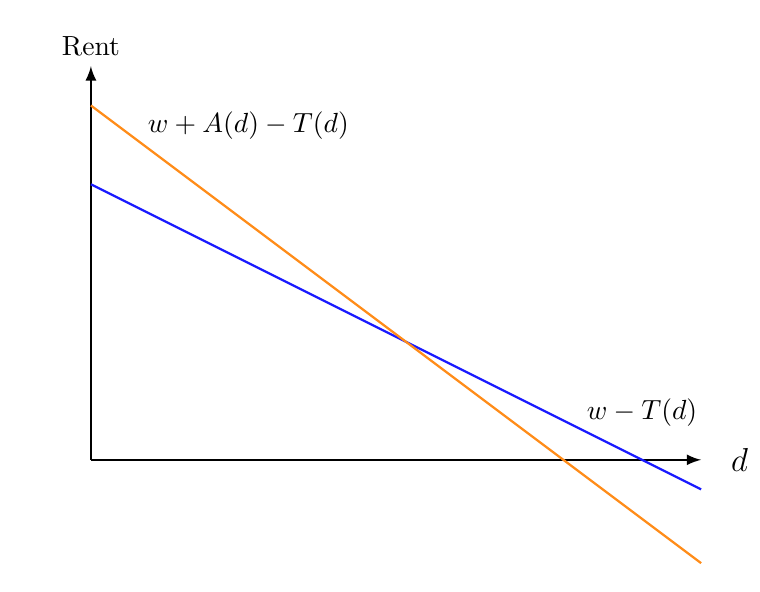
\begin{tikzpicture}[scale=.5]
\def\bndmax{5}        %https://tex.stackexchange.com/questions/68462/filling-a-complex-region-with-tikz
\def\bndmin{0.2}
\def \n {10}
\def \m {15.5}
\def \t {.5}
\def \th {1}
\def \w {7}
\tikzset{func/.style={thick,color=blue!90}}	
\draw [thick, latex-] (0,\n)node[above] {Rent}--(0,0);
\draw [thick, -latex] (0,0)--(\m,0)node[right=.25]{\large $d$};
%\foreach \xi in {0,..., \m} \draw (\xi,0)--(\xi,-.1)node[below=1]{\small$\xi$};
%\foreach \yi in {1,...,\n} \draw (0,\yi)--(-.1,\yi)node[left]{$\yi$};
%%\foreach \i in {1,4,9,16} {
	\draw[func,domain=0:\m] plot [samples=200] (\x,{\w-\t*\x});
%	\draw[func,domain=0:\m, dashed] plot [samples=200] (\x,{\w+\azero-\th*\x+\aprime*\x});

\node at (14,1.2){$w-T(d)$};
\def \azero{2}
\def \aprime {-.25}	
\tikzset{func/.style={thick,color=orange!90}}	
	\draw[func,domain=0:\m] plot [samples=200] (\x,{\w+\azero-\t*\x+\aprime*\x});
\node at (4,8.5){$w +A(d)-T(d)$};
%\node at(-.8,2) [left]{base $2^1=$};
%\node at(-.8,1) [left]{$2^0=$};
%\draw[dotted] (0,2)--(1,2)--(1,0); 
 \end{tikzpicture}
\end{center}
\caption{Rent profile with amenities}
\label{fig-amenity}
\end{figure}

 This model can produce variations on the standard result in the Alonso model. Figure~\ref{fig-amenity} illustrates a linear amenity function, $\mathbb{A}(d|N)= a-b*d$, that is convenient for illustrative purposes.  It shows how a particular amenity function might affect the rent profile, and hence city size and it allows simple experiments with the effect of increasing population on city size, wages and rents. 

In this case, amenity falls below zero in the outer regions of the city and, the geographical size of the city will be smaller. With a linear function, this happens if $\frac{a}{b} < \frac{w}{t}$. (a smaller city would have a secondary effect on wages, since with fewer workers' marginal productivity would be higher and therefore wages would rise. This would partially offset the initial decline in population.)
There would be a band of land around the city with negative amenity for commuters.\footnote{The very simple graphical result rests on several assumptions - no other housing expense, housing all the same size, wages all equal, preferences identical, transportation costs.}

The far more likely case is that $A(d) > 0$ when $w-T(d)$ falls to zero. In this case there is a band of residents around the city, outside of the population commuting to work. They do not travel to work,  do not collect a wage, but still enjoy the amenity of being close to a city. This might be a population of retired persons enjoying occasional visits and healthcare facilities.


\subsection{Neighbourhood amenity}
In Figure~{fig-amenity} the source of the amenity is at the centre of the city. We can easily imagine an amenity profile that is high for some neigbourhoods and lower for others, as in  In Figure~\ref{fig-amenity2}. The jagged area below the orange line is rent accruing to landowners. The variable rent comes not from a desire to be close to the source of the wage income but from household demand for local amenity.  
\begin{figure}[tb]
\begin{center}
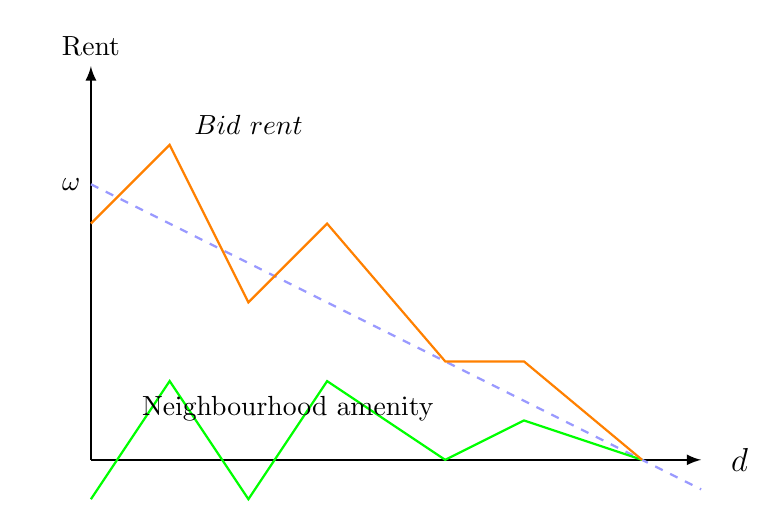
\begin{tikzpicture}[scale=.5]
\def\bndmax{5}        %https://tex.stackexchange.com/questions/68462/filling-a-complex-region-with-tikz
\def\bndmin{0.2}
\def \n {10}
\def \m {15.5}
\def \t {.5}
\def \th {1}
\def \w {7}
\tikzset{func/.style={thick,dashed, color=blue!40}}	
\draw [thick, latex-] (0,\n)node[above] {Rent}--(0,0);
\draw [thick, -latex] (0,0)--(\m,0)node[right=.25]{\large $d$};
% Basic Bid rent,
\node at(-.5,\w) {$\omega$};
\draw[func,domain=0:\m] plot [samples=200] (\x,{\w-\t*\x});
%NEIGBOURHOOD AMENITY
\draw [thick, green] (0,-1)--(2,2)--(4,-1)--(6,2)--(9,0)--(11,1)--(14,0);
\draw [thick, orange] (0,6)--(2,{7-2*.5+2})--(4,7-4*.5 -1)--(6,7-6*.5+2)--(9,7-9*.5)--(11,7-11*.5+1)--(14,7-14*.5);
\node [] at (5,1.3){Neighbourhood amenity};
\def \azero{2}
\def \aprime {-.25}	
% \tikzset{func/.style={thick,color=orange!90}}	
% 	\draw[func,domain=0:\m] plot [samples=200] (\x,{\w+\azero-\t*\x+\aprime*\x});
\node at (4,8.5){$Bid\ rent$};
%\node at(-.8,2) [left]{base $2^1=$};
%\node at(-.8,1) [left]{$2^0=$};
%\draw[dotted] (0,2)--(1,2)--(1,0); 
 \end{tikzpicture}
\end{center}
\caption{Rent profile with neighbourhood amenities}
\label{fig-amenity2}
\end{figure}
Financialization might or might not affect neighbourhood amenity. If it does it might have its effect by changing the ownership mix.

\subsection{Public provision of amenities}

Previous sections suggest amenities may work as a wage subsidy, potentially increasing output. Since employers will not willingly pay for urban amenities, some amenities may be financed publicly. It is common to introduce the cost of generating amenities as a tax on residents.  Since public amenities may be \glspl{public good} in the economic sense, the municipal government may be able to achieve significant wage economies with a small public expenditure.

A simple way to incorporate publicly provided amenities to make an amenity function that proportional to a fraction of public revenue, which is a fraction $\tau$ of the land value when municipalities depend on property taxes. Assuming a uniform property tax rate, total property tax revenue in a circular city are approximately $\tau(\phi+2/3 \omega)\pi \frac{\omega}{c}^2$. We can therefore include in the buyer's maximum bid function a fraction if this value. Property investors would not include this amenity component, but it would affect their decisions because amenity raises their net rent.

Notice that because amenity raises property values, in Ontario it does not raise tax revenue because the property tax rate is adjusted to balance the budget. This creates perverse incentives for municipalities \cite{blaisPerverseCitiesHidden2011}.


\subsection{An amenity sector}
Producing amenities takes resources. Some fraction of the workforce must be engaged in producing the amenity services. A simple approach would be to assume that the base employment that we consider demands a layer of amenities that represent the additional fraction of the population needed to provide the amenities - say 10\%  

Larger cities can support larger and more varied amenities, so that effect of amenities on property values might be larger in larger cities. At the same time, there are apparently economies of scale in the production of amenities \cite{kaufmannScalingUrbanAmenities2022}. We have no strong prior about how in amenity sector would be affected by finacialization of housing.  An effect might work through changing ownership.


\section{Research on amenities}
% There is a great deal of research on amenities. In this subsection mention a few that seemed noteworthy. 
Most of the literature on amenities deals with livability and the benefits for the individual. There is a strand in the literature, however, that links amenities to growth. In 1954, for example, Edward Ullman \cite{ullmanAmenitiesFactorRegional1954} published  ``Amenities as a Factor in Regional Growth,'' an article that came to be seen in the geographical literature over the following 50 years as prescient \cite{walcottCommentsEdwardUllman2010} for introducing the notion that amenities could be an important mobility magnet. 

Many have since extended this approach. Richard Florida, in a series of articles and books beginning in 2002 \cite{floridaCreativeClassEconomic2014, floridaEconomicGeographyTalent2002, floridaCompetingAgeTalent2005} examined the notion that urban growth depended on attracting the creative class and that in turn rested in part on the amenities a city offered. A 2008  Statistics Canada study, `Cities and Growth: The Left Brain of North American Cities,' Beckstead et al \ found substantial differences in average growth for cities with higher cultural employment and urban amenities.  Clark et al \cite{clarkAmenitiesDriveUrban2002} argue that much of Chicago's recent growth to 2003  should be attributed to reforms instituted by Mayor Richard M.  Daley explicitly linked to amenities and quality of life issues, including parks and schools. Abouy \cite{albouyWhatAreCities2016} finds that wage and housing cost differences across metropolitan areas are accounted for more by productivity than quality-of-life differences, however. 

Beckstead et al  \cite{becksteadCitiesGrowthLeft2008} identify amenities with the unexplained variastion in median urban house price after controlling for median household income.\footnote{  The basic premise would be that after conditioning on household income, variation in home prices across cities would be a function of the relative attractiveness of these places. The residuals yield a continuous ranking of cities based on the estimated variation in urban amenities.} Rappaport \cite{rappaportConsumptionAmenitiesCity2008} presents empirical evidence that amenities do support high-density levels, and that amenities cause approximately one-fifth of the cross-sectional variation in metro population density. 


% Molotch's (1976) metaphor suggests that the city is a machine geared to creating growth, with growth loosely defined as the intensification of land use and thus higher rent collections associated professional fees and locally based profits. Many urban economists, planners, and political scientists have made similar arguments (e.g., Bradbury, Downs, & Small, 1982; Mollenkopf, 1983; Stone, 1989). However, a quarter century later in the contemporary competition among US cities, the growth machine model has lost much of its power.
  


\newpage


\chapter{Notation}
% \section{Notation for Urban and Production Sectors}
\newpage
\begin{longtable}{lp{10cm}}
\caption{Notation}                       \\
\hline           &  \textbf{Productivity} \\ \hline
$K$              &  Capital               \\ 
% $L$            &  Labour                \\
$N$              &  Population, equals labour \\ %, $L$          
%$\Lambda$    &  Labour-augmenting agglomeration effect \\
$Y=A K^{\alpha }N^{\beta }$  &  a Cobb-Douglas Production function \\ %Urban output            \\
$\alpha$         &  Elasticity of output with respect to capital          \\
$\beta$          &  Elasticity of output with respect to labour           \\ % vs effective labour
$\gamma$         &  Elasticity of agglomeration with respect to labour    \\ % , $\Lambda(n)$, for illustration \\

% $L$              &  Labour supply \\ %the number of workers, which, in the standard circular city model, equals the number of lots of size $s$  when workers live on identical individual lots. % Unless $d^{max}>d^*$ v  \frac{\pi}{s}(\frac{w}{{c}})^2 =
$n$  &  Number of workers at a firm \\
% $n_i$  &  Number of workers employed by firm $i$ \\
%$n=\sum_i n_i$  &  Number of workers, the urban population in the model \\
% $\#f=\frac{n}{n_i}$&number of identical firms \\ %not used
% $f$  &  Number of firms =1 \\
% $n =f n_i$  &  Aggregate labour \\
% $n^\gamma$ & The labour-augmenting agglomeration effect,  modelled as an exponential function of the number of people \\
% $\Lambda(n)n_i$ &  Effective labour for firm $i$ \\
% $\Lambda'=\die{\Lambda(n)}{n} $ & Derivative of the labour-augmenting agglomeration effect\\

%%$Y_i=K_i^{\alpha }(\Lambda(n)n_i)^{\beta }$  &  Urban firm $i$'s output \\

%%$Y=\frac{n}{n_i}K_i^{\alpha }(\Lambda(\sum_i n_i)n_i)^{\beta }$  &  Aggregate output of all firms in the city \\
% $\die{Y}{n}=\beta\frac{1}{n} Y  \left( 1+ \frac{n\Lambda'}{\Lambda} \right)$  &  Social marginal product of labour \\
% $Y_i=K_i^{\alpha }(\Lambda(n)n_i)^{\beta }$    &  Urban firm $i$'s output \\
% $\die{Y_i}{K_i}	=\alpha \frac{1}{K_i} Y_i $  & Marginal product of capital for firm $i$ \\
% $\die{Y_i}{n_i}	=  \beta\frac{1}{n_i} Y_i $  &  Marginal product of labour for firm $i$ \\
%%$\eta=\frac{n_i\Lambda'}{\Lambda}$  &   Marginal agglomeration effect on a firm's output of increasing it's own labour stock \\
% \hline
	% &\textbf{Amenity}\\ \hline
% $A(d, n)$   &  Agglomeration amenity          \\

\hline  0 &  \textbf{Labour market}                \\ \hline %and urban stucture??
$\psi$            &  Rural subsistence wage                             \\  
$\omega$          &  Urban wage premium          \\
${c}$             &  Transportation cost per unit distance \\ % Was $\tau$, and $trans$. Considered $\gamma, \xi, \zeta$.
$d$               &  Distance from city centre   \\
$d^* = w/{c}$     &  City extent \\ %, the maximum distance commuters will travel \\ % Maximum distance commuters will travel \\ % to get the wage premium \\
% $\mathcal{R} = \omega - {dc}$ &  Rent at distance ${d}$ \\ 
% $\zeta$          &  Population density at distance $d$     \\
% $s$              &  Lot size      \\
% $\psi$  &  ?Per-period cost of a unit of productive capital \\
% $\omega + \psi$  &  Urban wage including rural wage \\ %***
% $\textit{t}$ & {\color{red}transportation cost per km} \\%use   c?
% $w^n=\omega-{dc}$ & Wage  premium net of transportation costs \\
%% $\Omega=\frac{\omega+\psi}{\psi}$  &  Ratio of the urban wage to the  cost of capital \\
%% $\Pi$	   &  Profit \\
%% $ER$	   &  Excess return to capital \\ 
% \hline &\textbf{Spatial structure in the circular city} \\ \hline		
%% $d^{max} = \omega /{c}$  &  Maximum distance commuters at which residents enjoy the urban amenity \\
%% $d^{**} = max(d^*, d^{max})$  &  radius of the city \\
%% $U$                     &  Worker utility **\\ %, a function of location and prices \\
%% $U^{urban}=U^{rural} $  &  Migration equilibrium assumption ** \\
% \hline & \textbf{Labour market} \\ 

\hline           & \textbf{Financial market}             \\ \hline
$P_W$            &  Warranted price for a property       \\
$P_B$            &  Bid price                            \\ % was P^{bid}
$P_A$            &  Asking price                         \\
$P_M$            &  Realized market price                \\
$P_M^e$          &  Expected market price                \\
% $P$            &  Price of a property                  \\ 
% $\dot P$       &  Rate of price growth              \\ % was $\dot p$  
% $\mathcal{C}$    &  Capital gains                     \\ % was C
% $\mathcal{C}_N$  &  Net capital gain, $C -$ net rent  \\
% $M$              &  Mortgage                          \\ 
% $m$              &  Mortgage share, the share of the property price that can be borrowed, which is a function of wealth  \\ 
$\mathcal{R}$    &  Rent                              \\
$\mathcal{R}_N$  &  Net rent                          \\
${R}^w_N$        &  Warranted rent                    \\
$\rho$           &  Rent ratio                        \\
$\phi$           &  \Gls{rent share}                  \\
$\mathcal{O}$    &  Operational costs                 \\
% $\theta$         &  Operations ratio                  \\ % was $\kappa$ became b
$\mathcal{T}$    &  Taxes                             \\ % was $\Sigma, \Xi$  
$\tau$           &  Property tax share                \\ % was t then $\sigma, \xi$  b
% $\tau$            &  Annual tax rate on rent and home \\ % Was $c$ 
$r$              &  Interest rate                     \\
$\delta$         &  Individual's subjective \gls{discount factor} \\
% $W$            &  Wealth                            \\
% $\psi$         &  Fraction with rent/operating costs\\
$t$              &  Time                              \\

W & Wealth \\
m & Mortgage share \\
M & Mortgage \\
S & Savings \\
% \mathbb{C} carrying 0.28, max_mortgage share, wealth_sensitivity

$\mathbb{T}$     &  Time period                       \\

$a$       &  Share of subsistence wage  used for land and building \\
$b$       &  Maintenance share of share of subsistence wage \\ % A cost. Includes water, electricity, heat? 
% $wage_share$     & OLD Share of the agglomeration effect that goes to workers. \\

\hline
\color{black}
\end{longtable}  

\newpage

\begin{longtable}{lp{10cm}}
\caption{Rent}                                                            \\
\hline
$\omega-{dc}$                &  Warranted (economic) rent                \\
$\mathcal{R}=\omega-{dc}$    &  Equilibrium rent payment of tenant       \\
PDV                           &  Present discounted value                 \\  
$\mathcal{R}^T$               &  PDV of rent collected over period $T$    \\ 
$\mathcal{R}^T_N=(1-\kappa-\sigma)\mathcal{R}^T$  &  PDV of net rent collected over period $T$ \\
\hline
\end{longtable}

\begin{longtable}{lp{10cm}}
\caption{Bidding mechanism notation}                                          \\
\hline
$\mathcal{R}_N$  &  Net rent                                                  \\ % was NR
% $P_0$            &  Purchase price for a property                             \\
% $P^T_e$          &  Expected price at the end of period $T$                   \\
$r^{prime}$         &  Prime interest rate                                       \\
$r^{target}$     &  Investor or banks target interest rate, $\bar r + margin$ \\

$r_i$            &  Agent $i$'s personal borrowing rate                       \\
$r_i^T$          &  Agent $i$ interest rate compounded over a period $T$      \\
$r_i^{disc}$     &  Agent $i$'s subjective discount rate (which may equal $r_i$) \\
$r_\delta$       &  Discount rate                                             \\ % was $discr_i$
$\delta_i^T$     &  Discount factor for agent $i$ over period $T$             \\
$m^W$            &  Wealth-based share of home price a worker can mortgage    \\ % $= m_i(W_i)$
$m^\omega$       &  Income-based share of home price a worker can mortgage    \\ % IS_i   IS_i(\omega+\psi)$$
$m_i = min(m^W_i, m^\omega_i)$  & Mortgage, the share of home price worker $i$ can mortgage \\

\hline
\color{black}
\end{longtable}  
Notation: 
Agent counts and indices are subscripts.
Values related to time are superscripts, time as a continuous 
variable is small, a period is capitalized e.g. the period $T$ of some number of years. 
In general values are capitals, rates are small letters.

% It might be better to use the subscript $m$ for `market'.  for warranted rents



 


% GLOSSARIES (Lists of definitions, abbreviations, symbols, etc. provided by the glossaries-extra package)
% -----------------------------
\printglossary
\cleardoublepage
\phantomsection		% allows hyperref to link to the correct page

%----------------------------------------------------------------------
\end{document} % end of logical document